\documentclass{book}
\usepackage{physics}
\usepackage{graphicx}
\usepackage{caption}
\usepackage{amsmath}
\usepackage{bm}
\usepackage{authblk}
\usepackage{amsfonts}
\usepackage{esint}
\usepackage{centernot}
\usepackage{mathtools}
\usepackage{bigints}
\usepackage{amsthm}
\theoremstyle{definition}
\newtheorem{defn}{Definition}[section]
\newtheorem{prop}{Proposition}[section]
\newtheorem{rmk}{Remark}[section]
\newtheorem{thm}{Theorem}[section]
\newtheorem{exmp}{Example}[section]
\newtheorem{prob}{Problem}[section]
\newtheorem{sln}{Solution}[section]
\newtheorem*{prob*}{Problem}
\newtheorem{exer}{Exercise}[section]
\newtheorem*{exer*}{Exercise}
\newtheorem*{sln*}{Solution}
\usepackage{empheq}
\usepackage{hyperref}
\usepackage{tensor}
\usepackage{xcolor}
\hypersetup{
	colorlinks,
	linkcolor={black!50!black},
	citecolor={blue!50!black},
	urlcolor={blue!80!black}
}
\newcommand{\p}{\partial}
\newcommand{\R}{\mathbb{R}}
\newcommand{\C}{\mathbb{C}}
\newcommand{\lag}{\mathcal{L}}

\newcommand{\ham}{\mathcal{H}}

\newcommand{\I}{\mathcal{I}}
\newcommand{\K}{\mathcal{K}}
\newcommand{\F}{\mathcal{F}}
\newcommand{\w}{\omega}
\newcommand{\lam}{\lambda}
\newcommand{\al}{\alpha}
\newcommand{\be}{\beta}
\newcommand{\x}{\xi}

\newcommand{\G}{\mathcal{G}}

\newcommand{\f}[2]{\frac{#1}{#2}}

\newcommand{\ift}{\infty}

\newcommand{\lp}{\left(}
\newcommand{\rp}{\right)}

\newcommand{\lb}{\left[}
\newcommand{\rb}{\right]}

\newcommand{\lc}{\left\{}
\newcommand{\rc}{\right\}}


\newcommand{\V}{\mathbf{V}}
\newcommand{\U}{\mathcal{U}}
\newcommand{\Id}{\mathcal{I}}
\newcommand{\D}{\mathcal{D}}
\newcommand{\Z}{\mathcal{Z}}

%\setcounter{chapter}{-1}


\makeatletter
\renewcommand{\@chapapp}{Part}
%\renewcommand\thechapter{$\bf{\ket{\arabic{chapter}}}$}
%\renewcommand\thesection{$\bf{\ket{\arabic{section}}}$}
%\renewcommand\thesubsection{$\bf{\ket{\arabic{subsection}}}$}
%\renewcommand\thesubsubsection{$\bf{\ket{\arabic{subsubsection}}}$}
\makeatother



\usepackage{subfig}
\usepackage{listings}
\captionsetup[lstlisting]{margin=0cm,format=hang,font=small,format=plain,labelfont={bf,up},textfont={it}}
\renewcommand*{\lstlistingname}{Code \textcolor{violet}{\textsl{Mathematica}}}
\definecolor{gris245}{RGB}{245,245,245}
\definecolor{olive}{RGB}{50,140,50}
\definecolor{brun}{RGB}{175,100,80}
\lstset{
	tabsize=4,
	frame=single,
	language=mathematica,
	basicstyle=\scriptsize\ttfamily,
	keywordstyle=\color{black},
	backgroundcolor=\color{gris245},
	commentstyle=\color{gray},
	showstringspaces=false,
	emph={
		r1,
		r2,
		epsilon,epsilon_,
		Newton,Newton_
	},emphstyle={\color{olive}},
	emph={[2]
		L,
		CouleurCourbe,
		PotentielEffectif,
		IdCourbe,
		Courbe
	},emphstyle={[2]\color{blue}},
	emph={[3]r,r_,n,n_},emphstyle={[3]\color{magenta}}
}


\begin{document}
\begin{titlepage}\centering
 \clearpage
 \title{{\textsc{\textbf{Topics in Quantum Theory}}}\\ \smallskip - A Quick Guide - \\}
 \author{\bigskip Huan Q. Bui}
  \affil{Colby College\\$\,$\\ PHYSICS \& MATHEMATICS\\ Statistics \\$\,$\\Class of 2021\\}
 \date{\today}
 \maketitle
 \thispagestyle{empty}
\end{titlepage}

\subsection*{Preface}
\addcontentsline{toc}{subsection}{Preface}

Greetings,\\

This text is my reading notes from \textit{Principles of Quantum Mechanics, Second Edition} by Shankar, \textit{Introductory Quantum Optics}, \textit{Optical Coherence \& Quantum Optics}, and \textit{Quantum Field Theory in a Nutshell} by Zee. Additional material comes from my class notes, my comments/interpretations/solutions, and other books/articles/notes. There are three parts to this text, as the title suggests. The Quantum Mechanics part covers the principles of quantum mechanics and some quantum field theory. A majority of this part will be my reading notes from Shankar's and Zee's book. The other two topics parts cover selected phenomena in quantum optics and quantum information theory.  \\

Background in linear algebra and modern physics (two semesters recommended) will be very helpful. I will try to cover some of the mathematical background, but a lot of familiarity will be assumed. \\

Enjoy!

\newpage
\tableofcontents
\newpage





\chapter{QUANTUM MECHANICS}


\newpage


\section{Mathematical Introduction}

\subsection{Linear Vector Spaces}

We should familiar with defining characteristics of linear vector spaces at this point. Here are some important definitions/theorems again:

\begin{defn}
	A linear vector space $\textbf{V}$ is a collection of objects called \textit{vectors} for which there exists
	
	\begin{enumerate}
		\item A definite rule for summing, and
		\item A definite rule for scaling, with the following features:
		
		
		\begin{itemize}
			\item Closed under addition: for $x,y \in \V$, $x+y \in \V$.
			\item Closed under scalar multiplication: $x\in \V$, then $ax \in \V$ for some scalar $a$.
			\item Scalar multiplication is distributive. 
			\item Scalar multiplication is associative.
			\item Addition is commutative.
			\item Addition is associative.
			\item There exists a (unique) null element in $\V$.
			\item There exists a (unique) additive inverse. 
		\end{itemize}
	\end{enumerate}
\end{defn}


Vector spaces are defined over some field. The field can be real numbers, complex numbers, or it can also be finite. As for good practice, we will begin to label vectors with Dirac bra-ket notation. So, for instance, $\ket{v} \in \V$ denotes vector $v \in \V$. Basic manipulations of these vectors are intuitive:
\begin{enumerate}
	\item $\ket{0}$ is unique, and is the null element.
	\item $0\ket{V} = \ket{0}$.
	\item $\ket{-V} = -\ket{V}$.
	\item $\ket{-V}$ is a unique additive inverse of $\ket{V}$.
\end{enumerate} 

The reasons for choosing to use the Dirac notation will become clear later on. Another important basic concept is \textit{linear (in)dependence}. Of course, there are a number of equivalent statement for linear independence. We shall just give one here:

\begin{defn}
	A set of vectors is said to be linearly independent if the only linear relation 
	\begin{align}
	\sum^n_{i=1}a_i\ket{i} = \ket{0}
	\end{align}
	is the trivial one where the components $a_i = 0$ for any $i$. 
\end{defn}



The next two basic concepts are \textit{dimension} and \textit{basis}. 

\begin{defn}
	A vector space $\V$ has dimension $n$ if it can accommodate a maximum of $n$ linearly independent vectors. We denote this $n$-dimensional vector space as $\V^n$.
\end{defn}

We can show that 

\begin{thm}
	Any vector $\ket{v} \in \V^n$ can be written (uniquely) as a linear combination of any $n$ linearly independent vectors.  
\end{thm}


\begin{defn}
	A set of $n$ linearly independent vectors in a $n$-dimensional space is called a \textit{basis}. So if $\ket{1},\dots,\ket{n}$ form a basis for $\V^n$, then any $\ket{v}\in \V$ can be written uniquely as
	\begin{align}
	\ket{v} = \sum^n_{i=1}a_i\ket{i}.
	\end{align}
\end{defn}

It is nice to remember the following:
\begin{align}
\boxed{\text{Linear Independence} = \text{Basis} + \text{Span}}
\end{align}

When a collection of vectors span a vector space $\V$, it just means that any $\ket{v} \in \V$ can be written as a linear combination of (some of) these vectors. 


The algebra of linear combinations is quite intuitive. If $\ket{v} = \sum_i a_i\ket{i}$ and $\ket{w} = \sum_i b_i\ket{i}$ then 

\begin{enumerate}
	\item $\ket{v + w} = \sum_i (a_i + b_i)\ket{i}$.
	\item $c\ket{v} = c\sum_i a_i\ket{i} = \sum_i ca_i\ket{i}$.
\end{enumerate}



A linear algebra text will of course provide a much better coverage of these topics. 















\subsection{Inner Product Spaces}


A generalization of the familiar dot product is the \textit{inner product} or the \textit{scalar product}. An inner product between two vectors $\ket{v}$ and $\ket{w}$ is denoted $\braket{v|w}$. An inner product has to satisfy the following properties:

\begin{enumerate}
	\item Conjugate symmetry (or skew-symmetry):$\braket{v}{w} = \braket{w}{v}^*$.
	\item Positive semi-definiteness: $\braket{v}{v} \geq 0$.
	\item Linearity in ket: $\braket{v}{aw + bz} = a\braket{v}{w} + b\braket{v}{z}$.
	\item Conjugate-linearity in bra: $\braket{av + bz}{w} = \bar{a}\braket{v}{w} + \bar{b}\braket{z}{w}$.
\end{enumerate}




\begin{defn}
	An inner product space is a vector space with an inner product. 
\end{defn}


\begin{defn}
	$\innerproduct{v}{w} = 0 \iff \ket{v} \perp \ket{w}$. 
\end{defn}


\begin{defn}
	The \textit{norm} (or length) of $\ket{v}$ is defined as 
	\begin{align}
	\norm{v} = \sqrt{\braket{v}}.
	\end{align}
	Unit vectors have unit norm. Unit vectors are said to be \textit{normalized}.  
\end{defn}




\begin{defn}
	A set of basis vectors all of unit norm, which are pairwise orthogonal will be called an \textit{orthonormal basis} or ONB. 
\end{defn}


Let $\ket{v} = \sum_i a_i\ket{i}$ and $\ket{w} = \sum_i b_i \ket{j}$, then 
\begin{align}
\braket{v}{w} = \sum_i a_i^*b_i \braket{i}{j}.
\end{align}



\begin{thm}
	\textbf{Gram-Schmidt:} Given a linearly independent basis, we can form linear combinations of the basis vectors to obtain an orthonormal basis. 
\end{thm}

Suppose that the Gram-Schmidt process gives us an ONB then we have
\begin{align}
\braket{i}{j} = \delta_{ij}.
\end{align}
As a result,
\begin{align}
\braket{v}{w} = \sum_i v_i^*w_i.
\end{align}
Alternatively, we can think this as doing the standard inner products of vectors whose entries are the components of the vectors $\ket{v}$, $\ket{w}$ in the basis:
\begin{align}
\ket{v} \to \begin{bmatrix}
v_1\\v_2\\\vdots\\v_n
\end{bmatrix}\hspace{0.5cm}
\ket{w} \to \begin{bmatrix}
w_1\\w_2\\\vdots\\w_n
\end{bmatrix} \implies \braket{v}{w} = \begin{bmatrix}
v_1^* & v_2^* & \dots & v_n^*
\end{bmatrix}\begin{bmatrix}
w_1\\ w_2 \\\vdots \\ w_n
\end{bmatrix}.
\end{align}
We can also easily see that 
\begin{align}
\braket{v}{v} = \sum_i \abs{v_i}^2 \geq 0.
\end{align}

\subsection{Dual Spaces and Dirac Notation}
Here we deal with some technical details involving the \textit{ket} (the column vectors) and the \textit{bra} (the row vectors). Column vectors are concrete manifestations of an abstract vector $\ket{v}$ in a basis, and we can work backward to go from the column vectors to the kets. We can do a similar thing with the bra vectors - since there's nothing special about writing the entries is a column versus in a row. However, we will do the following. We know that associated with every ket $\ket{v}$ is a column vector. So let its adjoint, which is a row vector, be associated with the bra, called $\bra{v}$. Now, we have two vector spaces, the space of kets and the dual space of bras. There is a basis of vectors $\ket{i}$ for expanding kets and a similar basis $\bra{i}$ for expanding bras. 

\subsubsection{Expansion of Vectors in an ONB}
It is extremely useful for us to be able to express a vector in an ONB. Suppose we have a vector $\ket{v}$ in an ONB $\ket{i}$. Then, let $\ket{v}$ be written as
\begin{align}
\ket{v} = \sum_i v_i \ket{i}.
\end{align}
To find the components $v_i$, we take the inner product of $\ket{v}$ with $\ket{j}$:
\begin{align}
\braket{j}{v} = \sum_i v_i \braket{j}{i} = \sum_i v_i\delta_{ij} = v_j.
\end{align}
With this, we can rewrite the vector $\ket{v}$ in the basis $\ket{i}$ as
\begin{align}
\ket{v} = \sum_i \ket{i}\braket{i}{v}.
\end{align}



\subsubsection{Adjoint Operations}
Here is a few details regarding taking the adjoints of vectors. Suppose that
\begin{align}
\ket{v} = \sum_i v_i\ket{i} = \sum_i \ket{i}\braket{i}{v}.
\end{align}
Then,
\begin{align}
\bra{v} = \sum_i\ket{i}v_i^*.
\end{align}
Now, because $v_i = \braket{i}{v}$, we have $v_i^* = \braket{v}{i}$. Thus, 
\begin{align}
\bra{v} = \sum_i \braket{v}{i}\bra{i}.
\end{align}
In plain words, the rule for taking the adjoint is the following. To take the adjoint of an equation involving bras and kets and coefficients, reverse the order of all factors, exchanging bras and kets and complex conjugating all coefficients. 


\subsubsection{Gram-Schmidt process}
Again, the Gram-Schmidt process lets us convert a linearly independent basis into an orthonormal one. For a two-dimensional case, procedure is the following:
\begin{enumerate}
	\item Rescale the first by its own length, so it becomes a unit vector. This is the first (orthonormal) unit vector.
	\item Subtract from the second vector its projection along the first, leaving behind only the part perpendicular to the first. (Such a part will remain since by assumption the vectors are nonparallel).
	\item Rescale the left over piece by its own length. We now have the second basis vector: it s orthogonal to the first and of unit length.
\end{enumerate}

In general, let $\ket{I}, \ket{II}, \dots$ be a linearly independent basis. The first vector of the orthonormal basis will be
\begin{align}
\ket{1} = \f{\ket{I}}{\norm{\ket{I}}}.
\end{align}
For the second vector in the basis, consider
\begin{align}
\ket{2'} = \ket{II} - \ket{1}\braket{1}{II}.
\end{align}
We can see that $\ket{2'}$ is orthogonal to $\ket{1}$:
\begin{align}
\braket{1}{2'} = \braket{1}{II} - \braket{1}\braket{1}{II} = 0.
\end{align}
So dividing $\ket{2'}$ by its norm gives us, $\ket{2}$, the second element in the ONB. To find the third element in the ONB, we have to first make sure it is orthogonal to both $\ket{I}$ and $\ket{II}$, so let us consider
\begin{align}
\ket{3'}= \ket{III} - \ket{1}\braket{1}{III} - \ket{2}\braket{2}{III}.
\end{align}
Once again we have $\ket{3'}$ orthogonal to both $\ket{1}$ and $\ket{2}$. Normalizing $\ket{3'}$ gives us $\ket{3}$, the third element in the ONB. We can now see how this process continues to the last element. 



\subsubsection{Schwarz and Triangle Inequality}
Just two small yet very important details:
\begin{thm}
	Schwarz Inequality:
	\begin{align}
	\abs{\braket{v}{w}} \leq \norm{v}\norm{w}
	\end{align}
\end{thm}


\begin{thm}
	Triangle Inequality:
	\begin{align}
	\norm{v+w} \leq \norm{v} + \norm{w}.
	\end{align}
\end{thm}



\subsection{Subspaces, Sum and Direct Sum of Subspaces}
I'm not too happy with the definitions given by Shankar's book. He also uses the notation for direct sum to indicate vector space addition, which is very confusing. Any linear algebra textbook would provide better definitions. For equivalent statements about directness of vector space sums, check out my \href{https://huanqbui.com/LaTeX\%20projects/Matrix_Analysis/HuanBui_MatrixAnalysis.pdf}{Matrix Analysis} notes. 




\subsection{Linear Operators}
Again, a rigorous definition of an operator can be found in almost any linear algebra textbook. But here,we can simply think of an operator as just some linear transformation from a vector space to itself. Say, if $\Omega$ is some operator that sends $\ket{v}$ to $\ket{v'}$, we write
\begin{align}
\Omega\ket{v} = \ket{v'}.
\end{align}
By definition, $\ket{v}$ and $\ket{v'}$ are contained in the same vector space. Now, we note that $\Omega$ can also act on bras:
\begin{align}
\bra{v}\Omega = \bra{v'}.
\end{align}
But of course the order of writing things is different, and once again, $\bra{v}$ and $\bra{v'}$ are contained in the same (dual) space. 


Next, because $\Omega$ is linear, we have the following familiar rules:
\begin{align}
\Omega \alpha \ket{v_i} &= \alpha\Omega \ket{v_i}.\\
\Omega \{ \alpha \ket{v_i} + \beta\ket{v_j} \} &= \alpha\Omega\ket{v_i} + \beta\Omega \ket{v_j}.\\
\bra{v_i}\alpha\Omega &= \bra{v_i}\Omega \alpha\\
\{\bra{v_i}\alpha + \bra{v_j}\beta \}\Omega &= \alpha\bra{v_i}\Omega + \beta \bra{v_j}\Omega.
\end{align}


One of the nice features of linear operators is that the action of an operator is completely determined by what it does to the basis vectors. Suppose 
\begin{align}
\ket{v} = \sum_i v_i \ket{i}
\end{align}
and 
\begin{align}
\Omega\ket{i} = \ket{i'},
\end{align}
then
\begin{align}
\Omega \ket{v} = \sum_i \Omega v_i \ket{i}= \sum_iv_i \Omega\ket{i} = \sum_iv_i\ket{i'}.
\end{align}



The next point of interest is \textit{products} of operators. As we might have seen, operators don't always commute. A product of operators applied to a vector just means operators are applied in sequence. The \textit{commutator} of two operators $\Omega, \Lambda$ is defined as
\begin{align}
\Omega\Lambda - \Lambda\Omega \equiv \lb \Omega,\Lambda \rb.
\end{align}
In general, $\lb \Omega,\Lambda\rb$ is not zero. Suppose three operators $\Omega, \Lambda, \Theta$ are involved, then we have two useful relations:
\begin{align}
&\lb \Omega, \Lambda\Theta \rb = \Lambda\lb \Omega, \Theta \rb + \lb \Omega, \Lambda \rb \Theta\\
&\lb \Lambda\Omega, \Theta \rb = \Lambda\lb \Omega, \Theta \rb + \lb \Lambda, \Theta \rb \Omega.
\end{align}
We notice that the form resembles the chain rule in calculus. 





\subsection{Matrix Elements of Linear Operators}
One thing we will hear very often in quantum mechanics is the idea of matrix elements. The idea, it turns out, is very simple. Suppose we have a basis $\ket{i}$, and an operator $\Omega$ such that
\begin{align}
\Omega\ket{i} = \ket{i'}.
\end{align}
Then, for
\begin{align}
\ket{v} = \sum_i v_i \ket{i}, 
\end{align}
we have
\begin{align}
\Omega\ket{v} = \Omega \sum_i v_i \ket{i} = \sum_i v_i \Omega\ket{i} = \sum_i v_i \ket{i'}.
\end{align}
Because we know $\Omega$ and $\ket{i}$, $\ket{i'}$ is also known, as in its components in the basis $\ket{j}$ (un-primed) are known:
\begin{align}
\braket{j}{i'} = \bra{j}\Omega\ket{i} \equiv \Omega_{ji},
\end{align}
where the $n^2$ numbers $\Omega_{ji}$ are the matrix elements of $\Omega$ in this basis. Now, if
\begin{align}
\Omega\ket{v} = \ket{v'}
\end{align}
then the components of the transformed ket $\ket{v'}$ can be expressed in terms of the components of $\ket{v}$ and the matrix elements $\Omega_{ji}$:
\begin{align}
v_i' = \braket{i}{v'} = \bra{i}\Omega\ket{v} = \bra{i}\Omega \sum_j v_j \ket{j} = \sum_j v_j \bra{i}\Omega\ket{j} = \sum_j \Omega_{ij}v_j.
\end{align}
We can see the above equation in matrix form as well:
\begin{align}
\begin{bmatrix}
v_1'  \\ \vdots \\ v_n'
\end{bmatrix}
=
\begin{bmatrix}
\bra{1}\Omega\ket{1} &  \dots & \bra{1}\Omega\ket{n} \\
\vdots & \ddots & \vdots\\	
\bra{n}\Omega\ket{1} & \dots & \bra{n}\Omega\ket{n} \\
\end{bmatrix}
\begin{bmatrix}
v_1 \\ \vdots \\ v_n 
\end{bmatrix}.
\end{align}
The elements of the first column are simply the components of the first transformed basis vector $\ket{1'} = \Omega\ket{1}$ in the given basis. Likewise, the elements of the j$^{\text{th}}$ column represent the image of the j$^\text{th}$ basis vector after $\Omega$ acts on it. 


\subsection{Matrix Elements of Products of Operators}

To get the matrix elements of a product of two operators, we do the following. Suppose we have operators $\Omega$ and $\Lambda$, then
\begin{align}
(\Omega\Lambda)_{ij} = \bra{i}\Omega\Lambda\ket{j} = \bra{i}\Omega \mathcal{I} \Lambda \ket{j}.
\end{align}
Now, we observe that 
\begin{align}
\mathcal{I} = \sum_k \ket{k}\bra{k}. 
\end{align}
So, 
\begin{align}
(\Omega \Lambda)_{ij} = \sum_k \bra{i}\Omega\ket{k}\bra{k}\Lambda \ket{j} = \sum_k \Omega_{ik}\Lambda_{kj}.
\end{align}



\subsection{The Adjoint of an Operator}
Recall that for a scalar $\alpha$
\begin{align}
\bra{\alpha v} = \bra{v}\alpha^*,
\end{align}
then we have a similar thing with operators if
\begin{align}
\Omega\ket{v} = \ket{v'}
\end{align}
then 
\begin{align}
\bra{\Omega v} = \bra{v}\Omega^\dagger,
\end{align}
where $\Omega^\dagger$ is \textit{the} adjoint of $\Omega$. The relationship between $\Omega^\dagger$ and $\Omega$ can be seen in a basis. We consider the matrix elements of $\Omega^\dagger$ in a basis:
\begin{align}
(\Omega^\dagger)_{ij} = \bra{i}\Omega^\dagger \ket{j} = \bra{\Omega i}\ket{j} = \bra{j}\ket{\Omega i}^* = \bra{j} \Omega \ket{i}^* = \Omega_{ji}^*.
\end{align}
We see that
\begin{align}
\Omega^\dagger_{ij} = \Omega^*_{ji},
\end{align}
i.e., in matrix form, $\Omega^\dagger$ is the conjugate transpose of $\Omega$. 

The rule for taking adjoins of equations is rather simple: When a product of operators, bras, kets, ad explicit numerical coefficients is encountered, reverse the order of all factors and make the substitution $\Omega \leftrightarrow \Omega^\dagger$, $\ket{} \leftrightarrow \bra{}$, $a \leftrightarrow a^*$. 


\subsection{Hermitian, Anti-Hermitian, and Unitary Operators}

\begin{defn}
	An operator $\Omega$ is Hermitian $\iff \Omega = \Omega^\dagger$.
\end{defn}


\begin{defn}
	An operator $\Omega$ is anti-Hermitian $\iff \Omega = -\Omega^\dagger$.
\end{defn}

Shankar's book ignores a bigger class of operators called \textit{normal} operators. Normal operators commute with their adjoints. In a sense, normal operators act \textit{like numbers}. Hermitian (or self-adjoint) operators are a subset of normal operators. So, the number-likeness of normal operators carries over to Hermitian operators and anti-Hermitian operators as well. Hermitian and anti-Hermitian operators are like pure real and pure imaginary numbers. Just as every number maybe be decomposed into a sum of pure real and pure imaginary parts, it turns out that we can decompose every operator into its Hermitian and anti-Hermitian parts. 
\begin{align}
\Omega = \f{\Omega + \Omega^\dagger}{2} + \f{\Omega - \Omega^\dagger}{2}.
\end{align}
One can verify that the first terms is Hermitian, and the second term is anti-Hermitian. 




\begin{defn}
	An operator $\mathcal{U}$ is unitary $\iff \mathcal{U}\mathcal{U}^\dagger = \mathcal{I}$. 
\end{defn}

Unitary operators are like complex numbers of unit modulus. 


\begin{thm}
	Unitary operators preserves the inner product between the vectors they act on.
	\begin{proof}
		Suppose
		\begin{align}
		\ket{v'} &= \mathcal{U}\ket{v}\\
		\ket{w'} &= \mathcal{U}\ket{w}.
		\end{align}
		Then
		\begin{align}
		\braket{v'}{w'} = \braket{\mathcal{U}v}{\mathcal{U}w} = \bra{v}\mathcal{U}^\dagger\mathcal{U}\ket{w} = \braket{v}{w}.
		\end{align}
	\end{proof}
\end{thm} 



\begin{thm}
	The columns (or rows) of a unitary matrix form an ONB.
	\begin{proof}
		Refer to a linear algebra text. The key is to consider an inner product between any two columns/rows.
	\end{proof}
\end{thm}


\subsection{Active and Passive Transformation}

Suppose all $\ket{v}$ is unitarily transformed to $\ket{v'}$:
\begin{align}
\ket{v} \to \U \ket{v}.
\end{align}
Then under this transformation, the matrix elements of any operator $\Omega$ are modified as follows:
\begin{align}
\ket{v'}\Omega\ket{v} \to \ket{\U v'} \Omega \ket{\U v} = \bra{v'}\U^\dagger \Omega \U \ket{v}.
\end{align}
It is clear that the same change is equivalent to leaving the vectors alone and subjecting all operators to the change
\begin{align}
\Omega \to \U^\dagger \Omega \U.
\end{align}

\textit{Active transformation} refers to changing the vectors, while \textit{passive transformation} refers to changing the operators.





\subsection{The Eigenvalue Problem}
I won't say much about what eigenvectors and eigenvalues are because we should be familiar with these concepts at this point. But just to introduce some terminology, each operator has certain kets of its own called \textit{eigenkets}, on which its action is simply that of scaling. So, eigenkets are just a different word for eigenvectors of an operator:
\begin{align}
\Omega\ket{v} = \omega\ket{v}.
\end{align}

Shankar's book talks about the characteristic equation and characteristic polynomial. While these are legitimate ways to find eigenvalues and eigenvectors, it is often very difficult. I'd prefer Leo Livshits' and Sheldon Axler's way and use minimal polynomials instead. I would steer away from determinants and characteristic polynomials at this point. 


\begin{thm}
	Eigenvalues of a Hermitian operator are real. 
	\begin{proof}
		Suppose 
		\begin{align}
		\Omega\ket{w} = a\ket{w},
		\end{align}
		then
		\begin{align}
		\bra{w}\Omega\ket{w} = a\braket{w},
		\end{align}
		and thus
		\begin{align}
		a^* \braket{w} = \bra{w}\Omega^\dagger\ket{w} = \bra{w}\Omega\ket{w} = a\braket{w}.
		\end{align}
		So we have
		\begin{align}
		(a - a^*)\braket{w} = 0.
		\end{align}
		Because $\ket{w}$ are eigenkets, they are cannot be the zero vector. This means $a = a^*$.
	\end{proof}
\end{thm}


Some might worry about the existence of eigenvalues of Hermitian operators. But worry no more, because Hermitian operators are a subclass of normal operators, which are a subclass of diagonalizable operators. This simply says Hermitian matrices are diagonalizable, and all its eigenvalues are real. But it turns out there is a little bit more to this. 


\begin{thm}
	For every Hermitian operator $\Omega$, there exists an ONB comprised entirely of the eigenvectors of $\Omega$. 
\end{thm}

Once again, this should be no surprise if one has studied normal operators. Hermitian operators inherit this property from its normalness. This property of normal operators are called the Spectral Theorem (for normal operators, of course). The proof of all this can be found in many linear algebra texts. 


\begin{thm}
	The eigenvalues of a unitary operator are complex numbers of unit modulus. 
	\begin{proof}
		The key to the proof is using inner products. 
	\end{proof}
\end{thm}



\subsubsection{Simultaneous Diagonalization of Two Hermitian Operators}

I would say the topic of simultaneous diagonalizability is covered quite well in Leo Livshits' course and hence in my \href{https://huanqbui.com/LaTeX\%20projects/Matrix_Analysis/HuanBui_MatrixAnalysis.pdf}{Matrix Analysis} notes. But here I will just give the most important results. 

\begin{thm}
	If $\Omega$ and $\Lambda$ are two commuting Hermitian operators, there exists a basis of common eigenvectors that diagonalizes them both. 
\end{thm} 

This result is not too surprising if we have studied simultaneous diagonalizability before. A more general theorem says that 
\begin{align}
\text{Simultaneous diagonalizbility} \iff \text{Individual diagonalizability} + \text{Commutativity}.
\end{align}
It is clear that because all Hermitian operators are diagonalizable, if two Hermitian operators commute, they are simultaneously diagonalizable.



\subsubsection{The Propagator}

In quantum mechanics (and classical mechanics of course), it is quite common to have some final state vector be obtained from an initial state vector multiplied by some matrix, which is independent of the initial state. We call this matrix the \textit{propagator}. 


The central problem in quantum mechanics is finding the state of a quantum system $\ket{\psi}$, which obeys the Schr\"{o}dinger equation:
\begin{align}
i\hbar \ket{\dot{\psi}} = J\ket{\psi}
\end{align}
where the Hermitian operator $H$ is called the \textit{Hamiltonian}. We will see much more of this as we move on.



\subsection{Functions of Operators and Related Concepts}


In this section, we look at whether it makes sense to define functions of operators. We will only restrict ourselves to functions that can be written as a power series. Consider a series
\begin{align}
f(x) = \sum_{n=0}^\infty = a_n x^n
\end{align}
where $x$ is a scalar. We defined the same function of an operator to be
\begin{align}
f(\Omega) = \sum_{n=0}^\infty a_n\Omega^n.
\end{align}
Now, this definition only makes sense if we have convergence. Consider this example:
\begin{align}
e^\Omega = \sum^\infty_{n=0}\f{\Omega^n}{n!},
\end{align}
where $\Omega$ is Hermitian. In the eigenbasis of $\Omega$, $\Omega$ is diagonal. This means we can add and/or take powers of $\Omega$ by add and/or take powers of the diagonal entries. We can find that
\begin{align}
e^\Omega = \begin{bmatrix}
\sum^\infty_{m=0}\f{\omega^m_1}{m!}&&\\
&&\\
&&\sum^\infty_{m=0}\f{\omega^m_n}{m!}
\end{bmatrix}
\end{align}
where $\omega_i$ are the eigenvalues of $\Omega$. We note that each entry in the expression above converges to $e^{\omega_i}$.



\subsubsection{Derivatives of Operators with Respect to Parameters}
Now, consider some operator $\Theta(\lambda)$ that depends on a parameter $\lambda$. The derivative of $\Theta$ with respect to $\lambda$ is defined to be
\begin{align}
\f{d\Theta(\lambda)}{d\lambda} = \lim_{\Delta\lambda \to 0} \lb \f{\Theta(\lambda + \Delta \lambda) - \Theta(\lambda)}{\Delta \lambda} \rb.
\end{align}
If $\Theta(\lambda)$ is written as a matrix, then the matrix of $d\Theta/d\lambda$ is obtained by differentiating the matrix elements of $\Theta(\lambda)$. A case that might be interesting to us is 
\begin{align}
\Theta(\lambda) = e^{\lambda\Omega}.
\end{align}
It turns out that if $\Omega$ is Hermitian or ``nice enough'' then 
\begin{align}
\f{d\Theta(\lambda)}{d\lambda} = \Omega e^{\lambda\Omega} = e^{\lambda\Omega}\Omega = \Theta(\lambda)\Omega = \Omega \Theta(\lambda).
\end{align}
Conversely, if we have
\begin{align}
\f{d\Theta(\lambda)}{d\lambda} = \Theta(\lambda)\Omega
\end{align}
then 
\begin{align}
\Theta(\lambda) = ce^{\lambda\Omega}
\end{align}
where $c$ is some operator. But we have to be careful that $c$ might not commute with $e^{\lambda\Omega}$.

The business of whether two operators commute or don't can make things slightly more complicated. If $\Theta$ and $\Omega$ commute, i.e., $[\Theta, \Omega] = 0$, then the rules of exponentiation carries over very nicely:
\begin{align}
&e^{a\Omega}e^{b\Omega} = e^{(a + b)\Omega}\\
&e^{a\Omega}e^{b\Theta} = e^{a\Omega + b\Theta}\\
&e^{a\Omega}e^{b\Theta}e^{-a\Omega} = e^{b\Theta}.
\end{align}
If $[\Omega, \Theta] \neq 0$, then the second and third equations no longer hold. Likewise, in differentiating a product, we have to be extra careful:
\begin{align}
\f{d}{d\lambda}e^{\lambda\Omega}e^{\lambda\Theta} = \Omega e^{\lambda\Omega}e^{\lambda\Theta} + e^{\lambda\Omega}e^{\lambda\Theta}\Theta.
\end{align}
While $[\Omega, e^{\lambda\Omega}] = 0$, because $\Theta$ and $\Omega$ might not commute, we can't bring $\Omega$ over to the right of $e^{\lambda\Theta}$. 


\subsection{Generalization to Infinite Dimensions}


\subsubsection{The Dirac delta function}
Consider the ordered $n$-tuple $\{ f_n(x_1), \dots, f_n(x_n) \}$ as components of a ket $\ket{f_n}$ in a vector space $\V^n(\mathbb{R})$:
\begin{align}
\ket{f_n} \leftrightarrow \begin{bmatrix}
f_n(x_1) \\ \vdots \\ f_n(x_n)
\end{bmatrix}.
\end{align}
The basis vectors in this space are:
\begin{align}
\ket{x_i} \leftrightarrow \begin{bmatrix}
0 \\ 0 \\ \vdots \\ 1 \\ 0 \\ \vdots \\ 0
\end{bmatrix} \leftarrow i^{th} \text{place}.
\end{align}
The basis vectors satisfy \textit{orthogonality} and \textit{completeness}:
\begin{align}
&\braket{x_i}{x_j} = \delta_{ij}\\
&\sum_{i=1}^n \ket{x_i}\bra{x_i} = \Id.
\end{align}
With this,
\begin{align}
\ket{f_n} = \sum_{i=1}^n f_n(x_i)\ket{x_i}.
\end{align}
We next define the inner product in this space:
\begin{align}
\braket{f_n}{g_n} \ sum^n_{i=1}f_n(x_i)g_n(x_i).
\end{align}
The functions $f_n$ and $g_n$ are said to be orthogonal if $\braket{f_n}{g_n} = 0$. We also have that
\begin{align}
\braket{f_n}{f_n} = \sum^n_{i=1}[f_n(x_i)]^2.
\end{align}
For finite $n$, nothing ``bad'' can really happen here. But what if $n$ is infinity? What we need is the redefinition of the inner product for finite $n$ in such a way that as $n$ goes to infinity, we get a smooth limit. A natural choice is
\begin{align}
\braket{f_n}{g_n} = \sum^n_{i=1} f_n(x_i)g_n(x_i)\f{L}{n+1}
\end{align}
where $L$ is the length of the interval. If we now let $n$ go to infinity, we get
\begin{align}
&\braket{f}{g} = \int^L_0 f(x)g(x)\,dx\\
&\braket{f} = \int^L_0 f^2(x)\,dx.
\end{align}
Now, if we consider complex functions as well in some interval $a\leq x \leq b$, the inner product becomes:
\begin{align}
\braket{f}{g} = \int^b_a f^*(x)g(x)\,dx.
\end{align}
But what are the basis vectors in this space and are they normalized? We know that 
\begin{align}
\braket{x}{x'} = 0
\end{align}
if $x \neq x'$. But what if $x = x'$? It turns out that we cannot simply require $\braket{x}{x} = 1$. The best way to see this is to deduce the correct normalization. We start with the completeness relation:
\begin{align}
\int^b_a \ket{x'}\bra{x'}\,dx' = \Id. 
\end{align}
Now, consider this
\begin{align}
\int^b_a \braket{x}{x'}\braket{x'}{f}\,dx' = \bra{x}\Id \ket{f} = \braket{x}{f}.
\end{align}
This is nothing but the projection of $\ket{f}$ along the basis ket $\ket{x}$, which is just $f(x)$. So, we also have $f(x') = \braket{x'}{f}$. Let the inner product $\braket{x}{x'}$ be some unknown function $\delta(x,x')$. Since $\delta(x,x')$ vanishes if $x\neq x'$, we can restrict the integral to an infinitesimal region near $x'=x$. With these, the equality above gives
\begin{align}\label{delt}
\int^{x+\epsilon}_{x-\epsilon}\delta(x,x')f(x')\,dx' = f(x).
\end{align}
In this infinitesimal region, $f(x)$ can assumed to be constant, and thus can be pulled out of the integral, leaving
\begin{align}
f(x)\int^{x+\epsilon}_{x-\epsilon} \delta(x,x')\,dx' = f(x).
\end{align}
And so we have
\begin{align}
\int^{x+\epsilon}_{x-\epsilon} \delta(x,x')\,dx' = 1. 
\end{align}
Clearly, $\delta(x,x')$ cannot be finite at $x=x'$. It should be infinite in such a way that its integral is 1. Since $\delta(x,x')$ depends only on the difference $x-x'$, we can write it as $\delta(x-x')$. So, the function $\delta(x-x')$ has the properties:
\begin{align}
\begin{cases}
\delta(x-x') = 0, \hspace{0.5cm} x \neq x'\\
\int^b_a \delta(x-x')\,dx' = 1\hspace{0.5cm} a < x < b
\end{cases}.
\end{align}
This is called the \textbf{Dirac delta function} and it fixes the normalization of the basis vectors:
\begin{align}
\braket{x}{x'} = \delta(x-x').
\end{align}

The Dirac delta function is ``strange'' in the sense that its value is either zero or infinite. It's thus useful to view it as the limit of a Gaussian:
\begin{figure}[!htb]
	\centering
	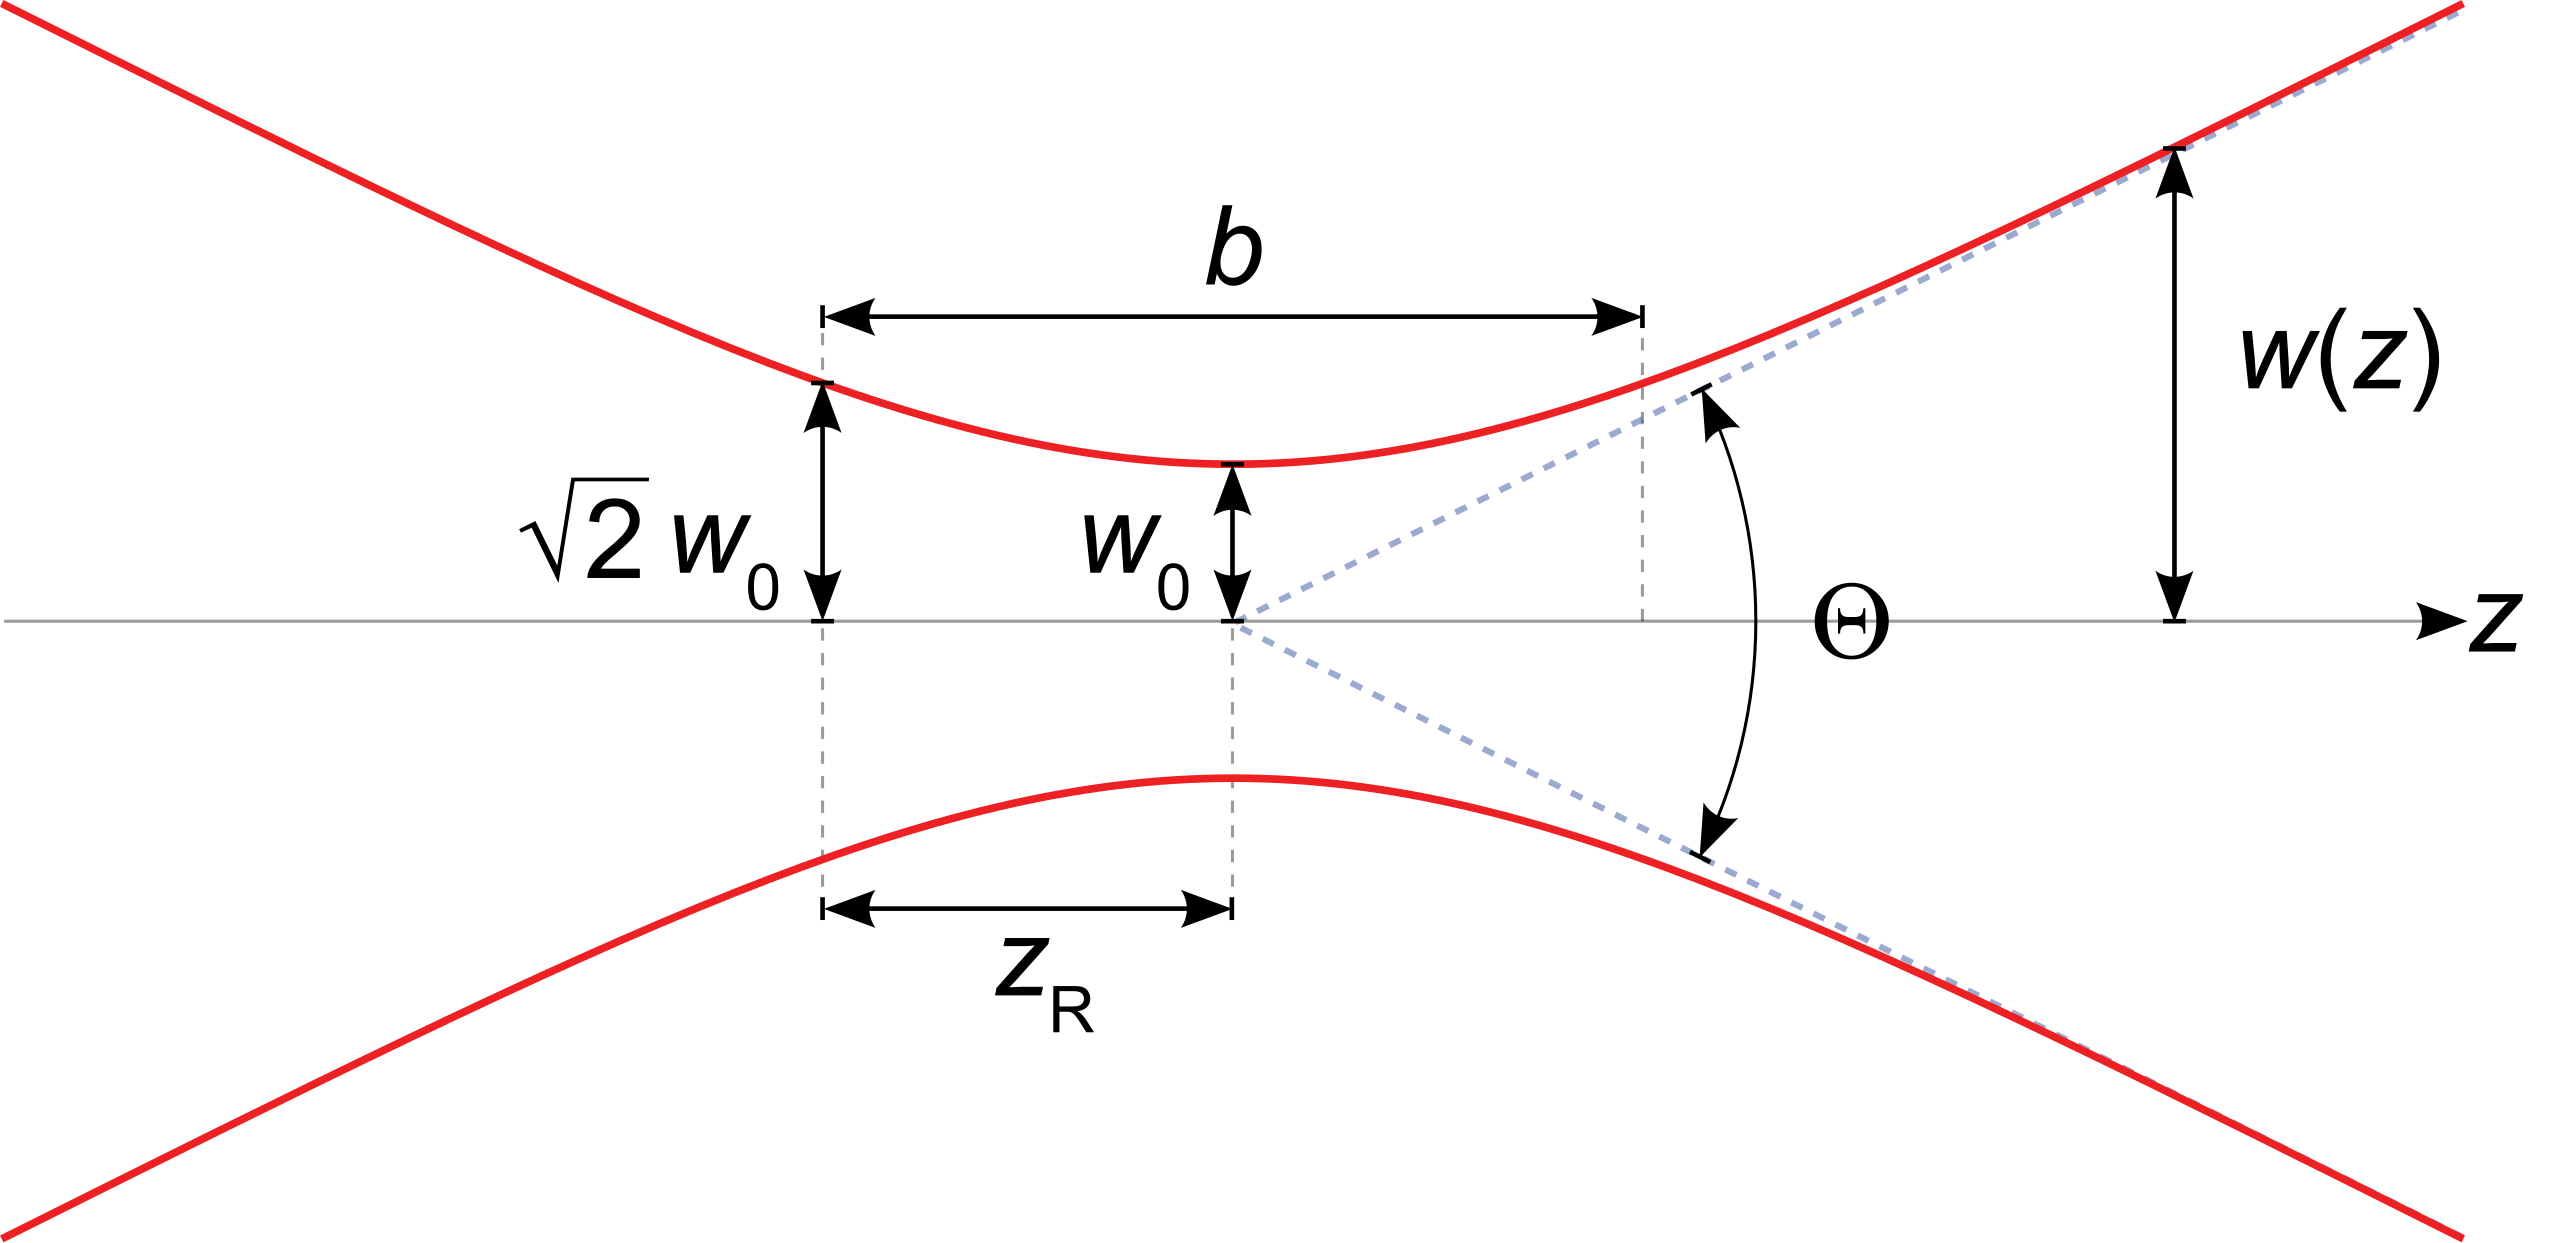
\includegraphics[scale=0.3]{gauss.png}
\end{figure}

of the form
\begin{align}
g_\Delta(x-x') = \f{1}{\sqrt{\pi \Delta^2}}e^{-(x-x')^2/\Delta^2}.
\end{align}
It is clear that the area under the curve is one (one can easily check this). Also, $\Delta \to 0$, $g_\Delta$ becomes closer and closer to $\delta(x-x')$ (the area under the curve is the same, while the width of the peak becomes smaller and smaller). 


From Gaussian model, we know that the delta function is not only real but also even:
\begin{align}
\delta(x-x') = \delta(x'-x).
\end{align}
Next, we consider the derivative of $\delta(x-x')$ with respect to $x$:
\begin{align}
\delta'(x-x') = \f{d}{dx}\delta(x-x') = -\f{d}{dx'}\delta(x-x').
\end{align}
Once again, we consider the Gaussian model. We consider $dg_\Delta(x-x')/dx = -dg_\Delta(x-x')/dx'$ as a function of $x'$:
\begin{figure}[!htb]
	\centering
	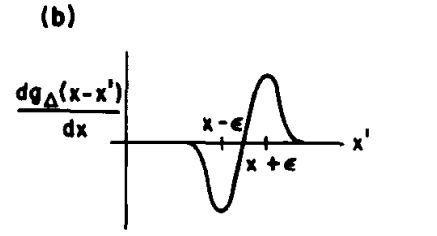
\includegraphics[scale=0.5]{dgauss.png}
\end{figure}

As $g_\Delta$ shrinks,, each bump at $\pm \epsilon$ will become, up to a scale factor, the $\delta$ function, such that
\begin{align*}
\int\delta'(x-x')f(x')\,dx' \propto   f(x+\epsilon) - f(x-\epsilon) = 2\epsilon\f{df}{dx'}\bigg\vert_{x=x'}.
\end{align*}
The constant of proportionality turns out to be $\epsilon/2$, and so
\begin{align}
\int \delta'(x-x')f(x')\,dx' = \f{df}{dx'}\bigg\vert_{x=x'} = \f{df(x)}{dx}.
\end{align}
In short, we can describe the $\delta'$ function as 
\begin{align}
\delta'(x-x') = \delta(x-x')\f{d}{dx'}.
\end{align}

In this way, we can describe higher derivatives of $\delta$:
\begin{align}
\f{d^n \delta(x-x')}{dx^n} = \delta(x-x')\f{d^n}{dx'^n}.
\end{align}



Next, we will develop an alternative representation of the delta function. Suppose we're given a function $f(x)$. The Fourier transform is given by 
\begin{align}
\F[f](k) = \f{1}{\sqrt{2\pi}}\int^\infty_{-\infty}e^{-ikx}f(x)\,dx.
\end{align}
And the inverse is given by
\begin{align}
\F^{-1}[f](x) = \f{1}{\sqrt{2\pi}}\int^\infty_{-\infty}e^{ikx'}f(k)\,dk.
\end{align}
Feeding the inverse formula into the transform formula, we get
\begin{align}
f(x') = \int^{\infty}_{-\infty} \lp \f{1}{2\pi} \int^{\infty}_{-\infty}e^{ik(x-x')\,dk} \rp f(x)\,dx.
\end{align}
Comparing this result to \eqref{delt}, we see that
\begin{align}
\boxed{\f{1}{2\pi}\int^\infty_{-\infty}e^{ik(x-x')\,dk} = \delta(x-x')}
\end{align}






\subsubsection{Operators in Infinite Dimensions}

Let us revisit the linear transformation:
\begin{align}
\Omega \ket{f} =\ket{\tilde{f}}
\end{align}
in the vector space whose basis is $\ket{x}$.

Let us assume that this action takes place in an infinite-dimensional vector space. Consider the differential operator. We can write the equation above as
\begin{align}
D_x\ket{f(x)} = \ket{df/dx}.
\end{align}

What are the matrix elements of the operator $D$ in the $\ket{x}$ basis? To find the matrix elements, we do exactly as before:
\begin{align}
\bra{x}D\ket{f} = \braket{x}{\f{df}{dx}} = \f{df(x)}{dx},
\end{align}
followed by
\begin{align}
\int \bra{x}D\ket{x'}\bra{x'}\ket{f}\,dx' = \f{df}{dx}.
\end{align}
We deduce that 
\begin{align}
\bra{x}D\ket{x'} = D_{xx'} = \delta'(x-x') = \delta(x-x')\f{d}{dx'}.
\end{align}

We notice that $D$ is not Hermitian because if
\begin{align}
D_{xx'} = D^*_{x'x}
\end{align}
then 
\begin{align}
D_{xx'} = \delta'(x-x') = D^*_{x'x} = \delta'(x'-x) = -\delta'(x-x'),
\end{align}
which is obviously not true. But we can convert $D$ to a Hermitian matrix by multiplying it with a purely imaginary number. Consider
\begin{align}
K = -iD.
\end{align}
Then
\begin{align}
K^*_{x'x} = [-i\delta'(x'-x)]^* = i\delta'(x'-x) = -i\delta'(x-x') = K_{xx'}.
\end{align}
It turns out that this is not enough to make $K$ Hermitian, as we shall show now. Suppose we have $\ket{f}$ and $\ket{g}$ in the function space whose images in the $x$ basis are $f(x)$ and $g(x)$ in the interval $a-b$. If $K$ is Hermitian, we must have that
\begin{align}
\bra{g}K\ket{f} = \bra{g}\ket{Kf} = \bra{Kf}\ket{g}^* = \bra{f}K^\dagger\ket{g}^* = \bra{f}K\ket{g}^*.
\end{align}
So, we ask
\begin{align}
\int^b_a \int^b_a \braket{g}{x}\bra{x}K\ket{x'}\braket{x'}{f}\,dx\,dx'  \stackrel{?}{=} \lp \int^b_a\int^b_a   \braket{f}{x}\bra{x}K\ket{x'}\braket{x'}{g}\,dx\,dx'  \rp^*.
\end{align}
Or, equivalently, we ask that if $K = -iD$, then
\begin{align}
 \int^b_a g^*(x)\lb -i\f{df(x)}{dx} \rb \,dx  \stackrel{?}{=}    \left\{ \int^b_a  f^*(x)\lb -i\f{dg(x)}{dx} \rb\,dx  \right\} = i\int^b_a \f{dg^*}{dx}f(x)\,dx.
\end{align}
Integrating the left hand side by parts gives
\begin{align}
-ig^*(x)f(x)\bigg\vert^b_a + i \int^b_a \f{dg^*}{dx}f(x)\,dx.
\end{align}
So for equality to hold, we require that 
\begin{align}\label{cond}
\boxed{-ig^*(x)f(x)\bigg\vert^b_a= 0}
\end{align}
Thus, in contrast to the finite-dimensional case, $K_{xx'} = K^*_{x'x}$ is not a sufficient condition for $K$ to be Hermitian. We must also look at the behavior of the functions at the end points $a$ and $b$. So what kinds of functions make this work? One set of such functions are the possible configurations $f(x)$ of the string clamped at $x=0$ and at $x=L$. These functions of course have zero boundary conditions. But this condition \eqref{cond} can also be fulfilled in another way. \\


Consider functions in 3-dimensional space, parameterized by $r,\theta,\phi$. Suppose that these functions are single-valued, say, $f(\theta) = f(\theta+2\pi)$. In the space of these functions, $K = -iD$ is Hermitian. This is very easy to verify since the condition \eqref{cond} is met:
\begin{align}
-ig^*(x)f(x)\big\vert_0^{2\pi} =-ig(2\pi)f(2\pi) + ig^*(0)f(0) = 0.
\end{align}

In quantum mechanics, we are interested in functions over the full interval $-\infty \leq x \leq \infty$. These functions into two classes: those that vanish at infinity and those that don't. Functions that don't vanish at infinity behave as $e^{-ikx}$, where $k$ is real. It is clear that if $K$ is sandwiched between two functions of the first class or two functions where one comes from each class, then $K$ is Hermitian, because the boundary terms vanish. But if $K$ is sandwiched between two functions of the second class, then whether $K$ is Hermitian depends on whether
\begin{align}
e^{ikx}e^{-ik'x}\bigg\vert_{-\infty}^\infty \stackrel{?}{=} 0.
\end{align}

If $k' = k$ then $K$ is Hermitian. If $k'\neq k$ then the answer is unclear because $e^{i(k-k')x}$ oscillates. It turns out that there exists a way of defining a limit for such functions that connect make up their minds: the limit as $\abs{x} \to \infty$. This limit is defined to be the average over a large interval. According to this prescription, we have, say as $x\to \infty$:
\begin{align}
\lim_{x\to\infty} e^{ikx}e^{-ik'x} = \lim_{L\to\infty, \Delta\to\infty}\f{1}{\Delta}\int^{L+\Delta}_L e^{i(k-k')x}\,dx = 0 \hspace{0.5cm} k\neq k'.
\end{align}
And thus $K$ is Hermitian in this space as well. \\

Next, we are interested in the eigenvalue problem of $K$. Let us start with
\begin{align}
K\ket{k} = k\ket{k}.
\end{align}
Following the standard procedure,
\begin{align}
\bra{x}K\ket{k} = k\braket{x}{k} &\implies \int \bra{x}K\ket{x'}\bra{x'}\ket{k}\,dx' = k\psi_k(x)\\ &\implies -i\f{d}{dx}\psi_k(x) = k\psi_k(x)
\end{align}
where $\psi_k(x) = \braket{x}{k}$. This is a very simple differential equation whose solution is
\begin{align}
\psi_k(x) = Ae^{ikx}.
\end{align}
Let us chose $A$ to be such that the function is normalized. In this case $A = 1/\sqrt{2\pi}$. And so,
\begin{align}
\ket{k} \sim \f{1}{\sqrt{2\pi}} e^{ikx},
\end{align}
and
\begin{align}
\braket{k}{k'} = \int^\infty_{-\infty} \braket{k}{x}\braket{x}{k'}\,dx = \f{1}{2\pi}\int^\infty_{-\infty}e^{-i(k-k')x}\,dx = \delta(x-x').
\end{align}


Now, because $K$ is Hermitian, functions that are expanded in the $x$ basis with components $f(x) = \braket{x}{f}$ must also have an expansion in the $K$ basis. What are the components in this expansion? We first look at the components in the $K$ basis, starting with $\ket{k}$:
\begin{align}
f(k) = \braket{k}{f} = \int^\infty_{-\infty} \braket{k}{x}\braket{x}{f}\,dx = \f{1}{\sqrt{2\pi}}\int^\infty_{-\infty} e^{-ikx}f(x)\,dx. 
\end{align}
To get back to the $x$ basis, we simply apply the inverse transform:
\begin{align}
f(x) = \braket{x}{f} = \int^\infty_{-\infty}   \braket{x}{k}\braket{k}{f}\,dk = \f{1}{\sqrt{2\pi}}\int^\infty_{-\infty} e^{ikx}f(k)\,dk.
\end{align}
Thus the familiar Fourier transform gives us the passage from one complete basis to another. What about the matrix elements of $K$ in the $k$ basis? It turns out that these elements are trivial:  
\begin{align}
\bra{k}K\ket{k'} = k'\braket{k}{k'} = k'\delta(k-k').
\end{align}
So, the $k$ basis is generated by the Hermitian operator $K$. So what generates the $x$ basis? Let us call this operator $X$, and that 
\begin{align}
X\ket{x} = x\ket{x}. 
\end{align}
Its matrix elements in the $x$ basis are
\begin{align}
\bra{x'}X\ket{x} = x\delta(x'-x).
\end{align}
To find its actions on functions, let us define
\begin{align}
X\ket{f} = \ket{\tilde{f}}.
\end{align}
And so
\begin{align}
\bra{x}X\ket{f} = \int  \bra{x}X\ket{x'}\bra{x'}\ket{f}\,dx' = xf(x) = \braket{x}{\tilde{f}} = \tilde(f)(x).
\end{align}
Therefore,
\begin{align}
\tilde{f}(x) = xf(x).
\end{align}
So, $X$ has the effect of multiplying a function $f$ by $x$:
\begin{align}
X\ket{f(x)} = \ket{xf(x)}.
\end{align}
We notice that there is a nice reciprocity between $X$ and $K$. Let us compute the matrix elements of $X$ in the $k$ basis:
\begin{align}
\bra{k}X\ket{k'} &= \f{1}{2\pi}\int^\infty_{-\infty} e^{-ikx} x e^{ik'x} \,dx \\
&= i\f{d}{dk} \lp \f{1}{2\pi}\int^\infty_{-\infty} e^{i(k'-k)x}\,dx \rp = i\delta'(k-k').
\end{align}
So, if $\ket{g(k)}$ is a ket whose image in the $k$ basis is $g(k)$ then
\begin{align}
X\ket{g(k)} = \ket{\f{idg(k)}{dk}}.
\end{align}

Thus we have the following. In the $x$ basis, $X$ acts as $x$. In the $k$ basis, $X$ acts as $-id/dx$. On the other hand, in the $k$ basis, $K$ acts as $k$, and in the $x$ basis as $-id/dk$. Operators with such an interrelationship are said to be \textbf{conjugate} of each other. Now, the conjugate operators $K$ and $X$ don't commute. Let us calculate their commutator. Suppose we have some ket $\ket{f}$. Then,
\begin{align}
&X\ket{f} \to xf(x)\\
&K\ket{f} \to -i\f{df(x)}{dx}.
\end{align} 
This is just the definition of these operators. Next,
\begin{align}
&XK\ket{f} \to -i x \f{df(x)}{dx}\\
&KX\ket{f} \to -i\f{d}{dx}xf(x).
\end{align}
Thus, 
\begin{align}
[X,K]\ket{f} \to -i x \f{df(x)}{dx} + i x \f{df(x)}{dx} + if \to i\Id\ket{f}.
\end{align}
So, we have for $X$ and $K$ conjugate of each other,
\begin{align}
[X,K] = i\Id.
\end{align}
























































\newpage


\section{Review of Classical Mechanics}


\subsection{Principle of Least Action \& Lagrangian Mechanics}

Suppose we have a particle in a potential $V(x)$. Newton tells us that
\begin{align}
m\f{d^2 x}{dt^2} = -\f{dV}{dx}.
\end{align}
In general coordinates,
\begin{align}
m_j \f{d^2x_j}{dt^2} = -\f{\p V}{\p x_j}.
\end{align}
In Lagrangian mechanics, we first define the \textit{Lagrangian}: $\lag = T - V$, where $T$ is the kinetic energy and $V$ is the potential energy. This makes $\lag = \lag(x,\dot{x},t)$. For each path connecting $(x_i,t_i)$ to $(x_f,t_f)$, the \textit{action} is given by
\begin{align}
S[x(t)] = \int^{t_f}_{t_i} \lag(x,\dot{x})\,dt.
\end{align}
The classical path which the particle follows is one which minimizes $S[x(t)]$. Variational methods (requiring $\delta S = 0$ and boundary terms to vanish) give us the \textbf{Euler-Lagrange equation(s)}:
\begin{align}
\boxed{\f{\p \lag}{\p x(t)} = \f{d}{dt}\f{\p \lag}{\p \dot{x}(t)}}
\end{align}
Details of this derivation can be found in many differential equation textbooks. We can easily show how Newton's Second law emerges from the Euler-Lagrange equation by setting $T = mv^2/2$. In which case, we get
\begin{align}
\f{d}{dt}(m\dot{x}) = m\ddot{x}= -\f{dV}{dx}.
\end{align}  
In general coordinates, we get the same thing:
\begin{align}
m\ddot{x}_{i} = -\f{\p V}{\p x_i}.
\end{align}
Now, we notice that we have assumed the potential $V$ to be velocity-independent. The force of a magnetic field $\mathbf{B}$ on a moving charge is excluded by this restriction ($\mathbf{F} = q\mathbf{v}\times \mathbf{B}$). We will show shortly how to accommodate this force in the Lagrangian formalism. However, this treatment will leave $\lag$ no longer in the form $T - V$. So, we will be free from the notion that $\lag$ has the form $T-V$, by only requiring that $\lag$ gives the correct equations of motion.

Suppose in some generalized coordinates, we have
\begin{align}
\f{d}{dt}\lp \f{\p \lag}{\p \dot{q}_i} \rp = \f{\p \lag}{\p q_i}.
\end{align}
It turns out that the \textit{form} of the Euler-Lagrange equation is invariant under change of coordinates. The Euler-Lagrange equation above can be made to resemble Newton's Second law if one defines a quantity:
\begin{align}
p_i = \f{\p \lag}{\p \dot{q}_i}
\end{align}
as the \textbf{canonical momentum conjugate to $q_i$} and the quantity
\begin{align}
F_i = \f{\p \lag}{\p q_i}
\end{align}
as the \textit{generalized force conjugate to $q_i$}. Note that these quantities are not always linear momentum and force. They can be angular momentum and torque, for instance. In many cases, we can find conservation laws from the Lagrangian, but we won't go into the details for now.









\subsection{The Electromagnetic Lagrangian}
As promised, in this subsection we will incorporate electromagnetism into the Lagrangian formalism. Recall that the force on a charge $q$ due to an electric field $\mathbf{E}$ and a magnetic field $\mathbf{B}$ is given by
\begin{align}
\boxed{\mathbf{F} = q\lp \mathbf{E} + \f{\mathbf{v}}{c}\times \mathbf{B} \rp}
\end{align}
where $\mathbf{v} = \dot{\mathbf{r}}$ is the velocity of the charged particle, and $c$ is the speed of light. It turns out that if we use 
\begin{align}
\boxed{\lag_{EM} = \f{1}{2}m\mathbf{v}\cdot\mathbf{v} - q\phi + \f{q}{c}\mathbf{v}\cdot\mathbf{A}}
\end{align}
we get the correct electromagnetic force laws. We note that $\phi$ and $\mathbf{A}$ are the scalar and the vector potentials related to $\mathbf{E}$ and $\mathbf{B}$ via:
\begin{align}
\mathbf{E} = -\grad{\phi} - \f{1}{c}\f{\p \mathbf{A}}{\p t}
\end{align}
and 
\begin{align}
\mathbf{B} = \curl{\mathbf{A}}.
\end{align}
With respect to this Lagrangian, the Euler-Lagrange equation is
\begin{align}
\f{d}{dt}\lp mx_i + \f{q}{c}\mathbf{A}_i \rp = -q\f{\p\phi}{\p x_i} + \f{q}{c}\f{\p \mathbf{v}\cdot\mathbf{A}}{\p x_i}.
\end{align}
We can combine the $i=1,2,3$ equations into one vector equation:
\begin{align}
\f{d}{dt}\lp m\mathbf{v} + \f{q\mathbf{A}}{c} \rp = -q\grad{\phi} + \f{q}{c}\grad{(\mathbf{v}\cdot\mathbf{A})}.
\end{align}
Rewriting this gives
\begin{align}
\f{d}{dt}m\mathbf{v} = -q\grad{\phi} + \f{q}{c}\lb -\f{d\mathbf{A}}{dt} + \grad{(\mathbf{v}\cdot\mathbf{A})} \rb
\end{align}


The canonical momentum is then
\begin{align}
\mathbf{p} = \f{\p \lag}{\p \dot{\mathbf{x}}} = m\mathbf{v} + \f{q\mathbf{A}}{c}. 
\end{align}
Now, the total derivative $d\mathbf{A}/dt$ has two parts:
\begin{align}
\f{d\mathbf{A}}{dt} = \f{\p \mathbf{A}}{\p t} + (\mathbf{v}\cdot \grad)\mathbf{A} 
\end{align}
where
\begin{align}
\lp\mathbf{v}\cdot\grad\rp_i = \f{dx_i}{dt}\f{\p}{\p x_i}.
\end{align}
Thus we have
\begin{align}
\f{d}{dt}m\mathbf{v} = -q\grad{\phi} - \f{q}{c}\f{\p \mathbf{A}}{\p t} + \f{q}{c}\lb \grad{(\mathbf{v}\cdot \mathbf{A})} - (\mathbf{v}\cdot \grad)\mathbf{A} \rb.
\end{align}
Now, we use the identity
\begin{align}
\mathbf{v}\times (\curl{A}) = \grad{(\mathbf{v}\cdot \mathbf{A})} - (\mathbf{v}\cdot \grad)\mathbf{A}
\end{align}
to get
\begin{align}
\f{d}{dt}m\mathbf{v} = -q\grad{\phi} - \f{q}{c}\f{\p \mathbf{A}}{\p t} + \f{q}{c}\mathbf{v}\times (\curl{A}).
\end{align}
Using the definition of $\mathbf{E}$ and $\mathbf{B}$ in relation to $\phi$ and $\mathbf{A}$ we indeed get the correct force law:
\begin{align}
\f{d}{dt}m\mathbf{v} = \mathbf{F} = q\lp \mathbf{E} + \f{\mathbf{v}}{c}\times\mathbf{B} \rp
\end{align}





\subsection{The two-body problem}
The two-body problem can be solved more elegantly in the \textit{center-of-mass coordinate system} where
\begin{align}
\mathbf{r} = \mathbf{r}_1 - \mathbf{r}_2
\end{align}
and 
\begin{align}
\mathbf{r}_{CM} = \f{m_1\mathbf{r}_1 + m_2\mathbf{r_2}}{m_1 + m_2}.
\end{align}
The inverse formulas are as follow:
\begin{align}
&\mathbf{r}_1 = \mathbf{r}_{CM} + \f{m_2\mathbf{r}}{m_1 + m_2}\\
&\mathbf{r}_2 = \mathbf{r}_{CM} - \f{m_1\mathbf{r}}{m_1 + m_2}
\end{align}
The original Lagrangian is
\begin{align}
\lag = \f{1}{2}m_1\abs{\dot{\mathbf{r}}_1}^2 + \f{1}{2}m_2\abs{\dot{\mathbf{r}}_2}^2 - V(\mathbf{r}_1 - \mathbf{r}_2). 
\end{align}
In CM coordinate system, the Lagrangian becomes:
\begin{align}
\lag =\f{1}{2}(m_1 + m_2)\abs{\dot{\mathbf{r}}_{CM}}^2 + \f{1}{2}\f{m_1m_2}{m_1+m_2}\abs{\mathbf{r}}^2 - V(\mathbf{r}).
\end{align}
By doing this, we have in a sense ``decoupled'' the problem:
\begin{align}
\lag(\mathbf{r},\dot{\mathbf{r}}, \mathbf{r}_{CM}, \dot{\mathbf{r}}_{CM},t) = \lag(\mathbf{r},\dot{\mathbf{r}},t) + \lag(\mathbf{r}_{CM}, \dot{\mathbf{r}}_{CM},t).
\end{align}
The first fictitious particle is the center of mass of the system. The motion of the center of mass is often uninteresting, so we can always go to the center of mass frame, so that the term $\lag(\mathbf{r}_{CM}, \dot{\mathbf{r}}_{CM},t)$ vanishes completely from the total Lagrangian. The second fictitious particle has \textit{reduced mass}:
\begin{align}
\mu = \f{m_1m_2}{m_1+m_2}
\end{align}
moves under the potential $V(\mathbf{r})$. Now, we only need to solve this one-body problem. 


\subsection{The Hamiltonian Formalism}
Recall the canonical momentum in Lagrangian mechanics:
\begin{align}
p_i = \f{\p \lag}{\p \dot{q}_i}.
\end{align}

In the Hamiltonian formalism one exchanges the roles of $\dot{q}$ and $p$: one replaces the Lagrangian $\lag(q,\dot{q})$ by a Hamiltonian $\ham(q,p)$ which generates the equations of motion, and $\dot{q}$ becomes a derived quantity:
\begin{align}
\dot{q}_i = \f{\p \ham}{\p p_i}.
\end{align}
But of course the question is, how can we make such a change? It turns out that there exists procedure for effecting such a change, called a \textit{Legendre transformation}. Suppose we have a function $f(x)$ with
\begin{align}
u(x) = \f{df(x)}{dx}.
\end{align}
How do we invert $u(x)$ to get $x(u)$? If we define a function (called the \textbf{Legendre transformation})
\begin{align}
\boxed{g(u) = x(u)u - f(x(u))}
\end{align}
then
\begin{align}
\f{dg}{du} = \f{dx}{du}u + x(u) - \f{df}{dx}\f{dx}{du} = x(u).
\end{align}
In going from $f$ to $g$, we simply exchange the roles of $x$ and $u$. $f$ and $g$ are called the Legendre transforms of each other. More generally, if $f = f(x_1,\dots,x_n)$, one can eliminate a subset $\{x_i\}$ in favor of the partial derivatives $u_i = \p f/\p x_i$ by the transformation
\begin{align}
g(u_1,\dots,u_j,x_{j+1},\dots,x_{n}) = \sum^j_{i=1}u_ix_i - f(x_1,\dots,x_n).
\end{align}
We can easily check that 
\begin{align}
\f{\p g}{\p u_i} = x_i.
\end{align}
So, we define the Hamiltonian as
\begin{align}
\boxed{\ham(q,p) = \sum^n_{i=1}p_i \dot{q}_i - \lag(q,\dot{q})}
\end{align}
where the $\dot{q}$'s are functions of $p$'s and $q$'s. Now, we observe that
\begin{align}
\f{\p \ham}{\p p_i} &= \f{\p }{\p p_i}\lp \sum^n_{j=1}p_j \dot{q}_j - \lag(q,\dot{q})  \rp\\
&= \dot{q}_i + \sum_{j=1}^n p_j \f{\p \dot{q}_j}{\p p_i} - \sum_{j=1}^n \underbrace{\f{\p \lag}{\p \dot{q}_j}}_{p_j}\f{\p \dot{q}_j}{\p p_i}\\
&= \dot{q}_i.
\end{align}
Similarly, we have that
\begin{align}
\f{\p \ham}{\p q_i} &= \f{\p }{\p q_i}\lp \sum^n_{j=1}p_j \dot{q}_j - \lag(q,\dot{q})  \rp\\
&= \sum_j p_j\f{\p \dot{q}_j}{\p q_i} - \f{\p \lag}{\p q_i} 
- \sum_j \underbrace{\f{\p \lag}{\p \dot{q}_j}}_{p_j}\f{\p \dot{q}_j}{\p p_i}
\\
&=-\f{\p \lag}{\p q_i}.
\end{align}
We obtain the \textit{Hamilton's canonical equations} by replacing $\p \lag / \p q_i$ by $\dot{p}_i$:
\begin{align}
\boxed{\f{\p \ham}{\p p_i} = \dot{q}_i, \hspace{0.5cm} -\f{\p \ham}{\p q_i} = \dot{p}_i}
\end{align}
We have altogether $2n$ first-order equations in time for a system with $n$ degrees of freedom. Given $(q_i(0), p_i(0))$ it is possible to integrate to find $(q_i(t), p_i(t))$.\\

Let us take a moment now to compare Lagrangian and Hamiltonian mechanics.\\

\noindent 
\begin{tabular}{|p{5.5cm}|p{5.5cm}|}
	\hline
	\textbf{Lagrangian formalism} & \textbf{Hamiltonian formalism}\\
	\hline
	The state of a system with $n$ df's is described by $n$ coordinates $(q_1,\dots,q_n)$ and $n$ velocities $(\dot{q}_1,\dots,\dot{q}_n)$, or in a more compact notation by $(q_i, \dot{q}_i)$. & The state of a system with $n$ df's is described by $n$ coordinates and $n$ momenta $(q_1,\dots,q_n; p_1, \dots, p_n)$ or, more succinctly, $(q,p)$.\\
	\hline
	The state of the system may be represented b a point moving with a definite velocity in an $n$-dimensional configuration space. & The state of the system nay be represented by a point in $2n$-dimensional phase space with coordinates $(q_1,\dots,q_n; p_1, \dots, p_n)$.\\
	\hline
	The $n$ coordinates evolve according to $n$ second-order equations.&The $2n$ coordinates and momenta obey $2n$ first-order equations.\\
	\hline
	For a given $\lag$, several trajectories may pass through a given point in configuration space depending on $\dot{q}$. & For a given $\ham$ only one trajectory passes through a given point in phase space.\\
	\hline
\end{tabular}\\



So what is $\ham$, physically? We know that $\lag$ can be interpreted as $T - V$ if the force is conservative. Let us looks at $\ham$ for this case. Suppose
\begin{align}
T &= \sum_{i=1}^n \f{1}{2}m_i \dot{x}_i^2 \\ p_i &= \f{\p \lag}{\p \dot{x}_i} = \f{\p T}{\p \dot{x}_i} = m_i \dot{x}_i,
\end{align}
where the coordinates are Cartesian $q_i = x_i$. This gives
\begin{align}
\ham 
&= \sum^n_{i=1}p_i \dot{x}_i - \lag(q,\dot{x})\\
&= \sum^n_{i=1}m_i \dot{x}_i^2 - \lag(q,\dot{x})\\
&= 2T - \lag\\
&= T + V.
\end{align}
So, we can interpret $\ham$ as the total energy (assuming that the force is conservative). Of course, we also assumed that the potential is not velocity-dependent, which does not apply to electromagnetism. In the next section, we will look into electromagnetism in the Hamiltonian scheme.
















\subsection{The Electromagnetic Force in the Hamiltonian Scheme}
Recall the Lagrangian for electromagnetism:
\begin{align}
\lag_{EM} = \f{1}{2}m\mathbf{v}\cdot\mathbf{v} -q\phi + \f{q}{c}\mathbf{v}\cdot\mathbf{A}
\end{align}
where 
\begin{align}
\mathbf{p} = m\mathbf{v} + \f{q\mathbf{A}}{c}.
\end{align}
In the Hamiltonian scheme, we write
\begin{align}
\ham_{EM} 
&= \mathbf{p}\cdot \mathbf{v} - \lag_{EM} \\
&= \lp m\mathbf{v} + \f{q\mathbf{A}}{c} \rp \cdot \mathbf{v} - \lp \f{1}{2}m\mathbf{v}\cdot\mathbf{v} -q\phi + \f{q}{c}\mathbf{v}\cdot\mathbf{A} \rp\\
&= \f{1}{2}m\mathbf{v}\cdot\mathbf{v} + q\phi\\
&= T + q\phi.
\end{align}
Wait a minute. What's happened to the vector potential $\mathbf{A}$? How can $\ham_{EM}$ generate the correct dynamics without knowing $\mathbf{A}$? It turns out that $T$ is dependent on $\mathbf{p}$ and $\mathbf{A}$. Recall that
\begin{align}
\f{1}{2}m\mathbf{v}\cdot\mathbf{v} = T = \f{\abs{\mathbf{p} - q\mathbf{A}/c}^2}{2m}.
\end{align}
Thus we have
\begin{align}
\boxed{\ham_{EM} = \f{\abs{\mathbf{p} - q\mathbf{A}/c}^2}{2m} + q\phi}
\end{align}





\subsection{Cyclic Coordinates, Poisson Brackets, and Canonical Transformations}
Let a Hamiltonian $\ham(q,p)$ be given. Suppose that the coordinate $q_i$ is missing in $\ham$, then 
\begin{align}
\dot{p}_i = -\f{\p \ham}{\p q_i} = 0,
\end{align}
which means the canonical momentum $p_i$ is conserved. Now, in many cases there are other quantities that are conserved, such as energy. How do we characterize these in the Hamiltonian formalism? It turns out there is a way to do this. \\

Suppose $\omega(q,p)$ is some state variable that doesn't depend explicitly on time $t$. Then we have by the chain rule
\begin{align}
\f{d\omega}{dt} 
&= \sum_i \lp \f{\p \omega}{\p q_i}\dot{q}_i + \f{\p \omega}{\p p_i}\dot{p}_i \rp\\
&= \sum_i \lp \f{\p \omega}{\p q_i}\f{\p \ham}{\p p_i} - \f{\p \omega}{\p p_i}\f{\p \ham}{\p q_i} \rp\\
&\equiv \{ \omega, \ham \}.
\end{align}
So, we define the Poisson bracket between two variables $\omega(q,p)$ and $\lambda(q,p)$ to be
\begin{align}
\boxed{\{\omega,\lambda\} = \sum_i \lp \f{\p \omega}{\p q_i}\f{\p \lambda}{\p p_i} - \f{\p \omega}{\p p_i}\f{\p \lambda}{\p q_i} \rp}
\end{align}

Let us look at this equation again
\begin{align}
\f{d\omega}{dt} = \sum_i \lp \f{\p \omega}{\p q_i}\f{\p \ham}{\p p_i} - \f{\p \omega}{\p p_i}\f{\p \ham}{\p q_i} \rp = \{ \omega, \ham \}
\end{align}
This says that any state variable whose Poisson bracket with $\ham$ vanishes is constant in time (i.e., is a conserved quantity). \\

Poisson brackets have a few important properties and similarities with commutators:
\begin{enumerate}
	\item $\{\omega, \lambda\} = -\{ \lambda,\omega    \}$
	\item $\{\omega, \lambda + \sigma \} = 
	\{\omega, \lambda  \}
	+
	\{\omega,  \sigma \}$
	\item $\{\omega, \lambda \sigma \} = 
	\{\omega, \lambda  \}\sigma
	+
	\lambda\{\omega,  \sigma \}$
	\item $\{ q_i,q_j \} = \{ p_i , p_j \} = 0$
	\item $\{ q_i, p_j  \} = \delta_{ij}$
	\item $\dot{q}_i = \{ q_i,\ham   \}$
	\item $\dot{p}_i = \{ p_i,\ham   \}$
\end{enumerate}

Please refer to Shankar's book for the sections on \textit{Canonical Transformations, Active Transformations, and Symmetries and Their Consequences}.

%\subsubsection{Canonical Transformations}
%\subsubsection{Active Transformations}
%\subsection{Symmetries and Their Consequences}
%\subsubsection{A Useful Relation between $\mathbf{S}$ and $\mathbf{E}$}




\newpage




%\section{All is Not Well with Classical Mechanics}
%\subsection{Particles and Waves in Classical Physics}
%\subsection{An Experiment with Waves and Particles (classical)}
%\subsection{The Double-Slit Experiment with Light}
%\subsection{Matter Waves (de Broglie Waves)}
%
%
%\newpage



\section{The Postulates \textendash a General Discussion}

\subsection{The Postulates}

Here we introduce the postulates of nonrelativistic quantum mechanics. We consider a system with one df (a particle in one dimension). The straightforward generalization to more particles in higher dimension will be introduced later. \\

\noindent
\begin{tabular}{|p{4cm}|p{7.2cm}|}
	\hline
	\textbf{Classical Mechanics} & \textbf{Quantum Mechanics}\\ \hline
	The state of a particle at any given time is specified by the two variables $x(t)$ and $p(t)$, i.e., as a point in a two-dimensional phase space. & The state of the particle is represented by a vector $\ket{\phi(t)}$ in a Hilbert space.\\ \hline
	Every dynamical variable $\omega$ is a function of $x$ and $p$: $\omega = \omega(x,p)$. & The independent variables $x$ and $p$ of classical mechanics are represented by Hermitian operators $X$ and $P$ with the following matrix elements in the eigenbasis of $X$: \begin{equation}
	\bra{x}X\ket{x'} = x\delta(x-x')
	\end{equation}
	\begin{equation}
	\bra{x}P\ket{x'}= -i\hbar\delta'(x-x').
	\end{equation}
	The operators corresponding to dependent variables $\omega(x,p)$ are given Hermitian operators
	\begin{equation} 
	\Omega(X,P) = \omega(x\to X, p \to P).
	\end{equation}\\ \hline
	If the particle is in a state given by $x$ and $p$, the measurement of the variable $\omega$ will yield a value $\omega(x,p)$. The state will remain unaffected. & If the particle is in a state $\ket{\psi}$, measurement of the variable corresponding to $\Omega$ will yield one of the eigenvalues $\omega$ with probability $P(\omega)\propto \abs{\braket{\omega}{\psi}}^2$. The state of the system will change from $\ket{\psi}$ to $\ket{\omega}$ as a result of the measurement.\\ \hline
	The state variables change with time according to Hamilton's equations: 
	\begin{equation}
	\dot{x} = \f{\p \ham}{\p \dot{p}}
	\end{equation}
	\begin{equation}
	\dot{p} = -\f{\p \ham}{\p x}
	\end{equation}
	&
	The state vector $\ket{\psi(t)}$ obeys the Schr\"{o}dinger equation 
	\begin{equation}
	i\hbar\f{d}{dt}\ket{\psi(t)} = H\ket{\psi(t)}
	\end{equation}
	where $H(X,P)=\ham(x\to X, p\to P)$ is the quantum Hamiltonian operator and $\ham$ is the Hamiltonian for the corresponding classical problem.\\\hline
\end{tabular}


\subsubsection{Collapse of the State Vector}
Suppose we have a state vector written in a general form

\begin{align}
\ket{\psi} = \sum_\omega \ket{\omega}\bra{\omega}\ket{\psi}
\end{align}
where $\ket{\omega}$ are of course the eigenstates. We recall that this expression is equivalent to writing $\ket{\psi}$ as a linear combination of the eigenstates $\ket{\omega}$ (where the corresponding eigenvalues are $\epsilon$), with coefficients being the inner product of $\ket{\psi}$ and $\ket{\omega}$, which we can think of as ``how much of $\ket{\psi}$ is in a certain $\ket{\omega}$'' direction. \\

Now, postulate III says that the measurement of the variable $\Omega$ changes the state vector. This phenomenon is called the \textit{collapse/reduction of the state vector}. There are two types of measurements in quantum mechanics. Loosely speaking, an \textit{ideal measurement} of $\Omega$ leaves only the eigenstates of $\Omega$ invariant. For example, \textit{ideal measurement} of the momentum of a particle in a momentum eigenstate leaves the state vector of the particle unchanged. Physically, this is due to the fact that the photons required for this measurement can be infinitesimally low in energy. On the contrary, suppose we want to \textit{ideally} measure the position of some particle in a momentum eigenstate $\ket{p}$, which we can write in terms of the position eigenstates as
\begin{align}
\ket{p} =\int \ket{x} {p}\,dx.
\end{align}
We see that the measurement forces the particle into some eigenstate $\ket{x}$, thus changing the state vector. 



\subsubsection{Expectation Value}

Suppose we want to measure a variable $\Omega$, given a large ensemble of $N$ particles in a state $\ket{\psi}$. Quantum theory allows us to predict how much of the population will yield some eigenvalue $\omega$. However, often we are interested in the \textit{expectation value} of these measurements, which is defined in statistics as
\begin{align}
\langle \Omega \rangle = \sum_i  \omega_i P(\omega_i).
\end{align}
But of course each probability is the modulus square of inner product of $\ket{\psi}$ and $\ket{\omega}$. So we can write the expectation value as
\begin{align}
\langle \Omega \rangle = \sum_i \omega_i \abs{\bra{\omega_i}\ket{\psi}}^2 = \sum_i \omega_i \braket{\psi}{\omega_i}\braket{\omega_i}{\psi}.
\end{align}
Now, because each $\omega_i$ is an eigenvalue corresponding to an eigenfunction $\ket{\omega_i}$ in the eigenvalue equation $\Omega\ket{\omega_i} = \omega_i\ket{\omega_i}$, we can rewrite the equation above as
\begin{align}
\sum_i  \bra{\psi}\Omega\ket{\omega_i} \braket{\omega_i}{\psi} = \bra{\psi} \Omega \lp\sum_i \ket{\omega_i}\bra{\omega_i}\rp \ket{\psi} = \bra{\psi}\Omega\ket{\psi},
\end{align}
by completeness. Thus, 
\begin{align}
\boxed{\langle \Omega \rangle = \bra{\psi}\Omega\ket{\psi}}
\end{align}
So, we notice a few things:
\begin{enumerate}
	\item To calculate $\langle \Omega \rangle$, we only need the operator $\Omega$. We do not need to know the eigenstates nor the eigenvalues of $\Omega$. 
	\item If the particles is in some eigenstate $\ket{\omega_i}$ of $\Omega$, then $\langle \Omega \rangle = \omega_i$, the corresponding eigenvalue. 
	\item $\langle \Omega \rangle$ is not necessarily one of the eigenvalues $\omega_i$. 
\end{enumerate}





\subsubsection{The Uncertainty}

Beside the mean (or the expectation value), another useful quantity to specify is the \textit{standard deviation}, or the \textit{uncertainty}. Statistically, it is defined as
\begin{align}
\Delta \Omega = \sqrt{\langle \Omega^2 \rangle - \langle \Omega \rangle^2}.
\end{align}
In quantum mechanics, if $\Omega$ has a discrete spectrum, then the uncertainty in $\Omega$ is given by
\begin{align}
\boxed{\Delta \Omega= \sqrt{ \sum_i P(\omega_i) (\omega_i - \langle \Omega \rangle)^2  }}
\end{align}
Else if it has a continuous spectrum, then
\begin{align}
\boxed{\Delta \Omega  = \sqrt{\int P(\omega)(\omega - \langle \Omega\rangle)^2\,d\omega}}
\end{align}
Or equivalently, we can write the uncertainty in $\Omega$ as a square root of an expectation value (this is all statistical definitions, by the way):
\begin{align}
\boxed{\langle \Omega\rangle = \sqrt{ \bra{\psi}  (\Omega - \langle \Omega \rangle)^2  \ket{\psi}}}
\end{align}










\subsubsection{Compatible and Incompatible Variables}


Suppose we want to measure some quantity $\Omega$ from the state $\ket{\psi}$. Such a measurement can yield an eigenvalue, say $\omega$, with probability $P(\omega)= \abs{\braket{\omega}{\psi}}^2$ where $\ket{\omega}$ is the eigenfunction corresponding to the eigenvalue $\omega$. Now, what if we want to measure a different variable, say $\Lambda$, on the already measured state $\ket{\psi}$? We see that this is sort of like a filtering process where we start with $\ket{\psi}$ and want to produce a state with $\omega$ and $\lambda$. But notice that once we measure $\ket{\psi}$, we have made the transformation $\ket{\psi} \to \ket{\omega}$. Can measuring $\ket{\omega}$ give $\ket{\lambda}$? The answer is no, not generally, since $\ket{\omega}$ must has a component that is the eigenfunction corresponding to the eigenvalue $\ket{\lambda}$. \\

An exception occurs when the state produced after the first measurement is unaffected by the second measurement, i.e., $\ket{\omega}$ is also an eigenstate of $\Lambda$. So, a natural question is when do two operators $\Omega$ and $\Lambda$ have \textit{exactly} the same eigenkets? Mathematically, we want to know when the following equation 
\begin{align}
[\Omega, \Lambda] = 0 \forall \text{ eigenket}
\end{align}
holds. Well, given any two operators $\Omega$ and $\Lambda$, we call $\Omega$ and $\Lambda$ \textit{compatible} if they commute, i.e., $[\Omega, \Lambda] = 0$. They are \textit{incompatible} when they don't commute. There's also a third situation where $\Omega$ and $\Lambda$ don't share all of their eigenkets. \\

If $\Omega$ and $\Lambda$, we can show with linear algebra that $\Omega$ and $\Lambda$ are simultaneously diagonalizable, i.e., we know a complete basis of simultaneous eigenkets can be found. \\

If $\Omega$ and $\Lambda$ never commute, then any attempt to filter $\Omega$ is ruined by a subsequent filtering for $\Lambda$ and vice versa. A classic example of this is the canonical commutation rule
\begin{align}
[\hat{x}, \hat{p}] = i\hbar,
\end{align}
which is the origin of the \textit{Heisenberg uncertainty principle}. \\

There's nothing interesting about the third situation so we will skip it. 






\subsubsection{The Density Matrix}

For an ensemble of $N$ systems, the \textit{density matrix} is given by
\begin{align}
\rho = \sum_i p_i \ket{i}\bra{i}
\end{align}
where
\begin{align}
p_i = \f{n_i}{N}
\end{align}
is the probability that a system picked randomly out of the ensemble is in the state $\ket{i}$.\\

Any ensemble average of $\Omega$ is given by
\begin{align}
\langle \bar{\Omega} \rangle = \sum_i p_i \bra{i}\Omega\ket{i}.
\end{align}
We note that there are two \textit{kinds} of average going on here. First we have $\bra{i}\Omega\ket{i}$, which is the expectation value of $\Omega$ for a given state $i$, and then we have the \textit{bar} average, which is the statistical expectation value over the entire ensemble. Next, we observe that
\begin{align}
\Tr(\Omega \rho) &= \sum_j \bra{j}\Omega \rho \ket{j}\\
&= \sum_j \sum_i    \bra{j}\Omega\ket{i}\bra{i}\ket{j}p_i\\
&= \sum_i \sum_j \braket{i}{j}\bra{j}\Omega\ket{i}p_i\\
&= \sum_i \sum_j \delta_{ij}  \bra{j}\Omega\ket{i}p_i\\
&= \sum_i p_i \bra{i}\Omega\ket{j}\\
&= \langle \bar{\Omega} \rangle.
\end{align}
Thus we say the density matrix contains all statistical information about the ensemble. Now, suppose we don't want $\langle $ but instead $\bar{P(\omega)}$, the probability of obtaining a particular value $\omega$, then we simply replace $\bar{\Omega}$ by an \textit{probability operator} for $\omega$, which is simply $\ket{\omega}\bra{\omega}$. So,
\begin{align}
\bar{P(\omega)} = \Tr(\ket{\omega}\bra{\omega} \rho).
\end{align}

Now, a very important property of the density matrix is that its trace is 1:
\begin{align}
\Tr(\rho) &= \sum_j \bra{j} \rho \ket{j} \\ 
&= \sum_j \bra{j}  \lp\sum_i \ket{i}\bra{i} \rp \ket{j}\\
&= \sum_j \sum_i \delta_{ij}\delta_{ij}\\
&= 1.
\end{align}

Since the density matrix is defined as a sum of outer products, it acts like a projection, and thus is Hermitian, i.e., $\rho^\dagger = \rho$. Any because it is a projection, letting it act twice (assuming ensemble is pure) is the same as letting it act once $\rho^2 = \rho$. If the ensemble is uniformly distributed over $k$ states then $\rho = (1/k)I$ where $I$ is the identity. And finally, $\tr(\rho^2) \leq 1$ in general, where equality holds when the ensemble is pure.






\subsection{The Schr\"{o}dinger Equation \& The Propagator}

At this point we should know what the Schr\"{o}dinger equation is and its solution for the SHO problem. But now let us look a bit closer in terms of Dirac brakets. Let the initial ket $\ket{\psi(0)}$ be given. How is it going to evolve in time? We find this by constructing a propagator $U(t)$ such that
\begin{align}
\ket{\psi(t)} = U(t)\ket{\psi(0)}.
\end{align}
We note that $U(t)$ must retain the normalization of $\ket{\psi}$, i.e., preserve the length of the vector $\ket{\psi}$. We have reasons to think that $U(t)$ is unitary. Now, the time-independent SE says
\begin{align}
\ham\ket{\psi} = E\ket{\psi}.
\end{align}
Suppose the eigenfunction corresponding to the eigenvalue $E$ is found to be $\ket{E}$. Then we can write $\ket{t}$ is the $\ket{E}$ basis:
\begin{align}
\ket{\psi(t)} = \sum c_i \ket{E_i} = \sum\ket{E} \bra{E}\psi(t)\ket \equiv \sum a_E(t)\ket{E}.
\end{align}
Now, let $\hat{H}$ act on both sides of the equation and using the fact that both $\ket\psi(t)$ and $\ket{E}$ are solutions to the SE to get
\begin{align}
i\hbar \dot{a}_E = Ea_E.
\end{align}
This is a rather easy ODE to solve. The general solution has the form
\begin{align}
a_E(t) = a_E(0)e^{-iEt/\hbar}.
\end{align}
Now, note that $a_E(t)$ are inner products between $\ket{E}$ and $\ket{\psi(t)}$. In other words, 
\begin{align}
\braket{E}{\psi(t)} = \braket{E}{\psi(0)}e^{-iEt/\hbar}.
\end{align}

Plugging everything back into the expression for $\ket{\psi(x)}$ we get
\begin{align}
\ket{\psi(t)} = \sum \ket{E}  \braket{E}{\psi(0)} e^{-iEt/\hbar}.
\end{align}


And thus we can now extract $U(t)$, where $\ket{\psi(t)} = U(t)\ket{\psi(0)}$:
\begin{align}\label{propagator}
\boxed{U(t) = \sum_E \ketbra{E}{E}e^{-iEt/\hbar}}
\end{align}


Now, by Taylor series expansion, we can verify that an expression for the propagator $U(t)$ is
\begin{align}
U(t) = e^{-i\ham t/\hbar},
\end{align}
where $\ham$ here is the Hamiltonian itself. Now, because $\ham$ is Hermitian (self-adjoint), $U(t)$ must be unitary, as expected. Thus we can think of the propagator $U(t)$ as some sort of a rotation of the vector $\ket{\psi}$ in Hilbert space. From linear algebra, we know that unitary operators preserves length. This is the reason why $\ket{\psi(t)}$ stays normalized once it is normalized at $t=0$. \\

Now, what if we chose to be in a different frame where the vectors $\ket{\psi}$ seem frozen (i.e. not rotating)? First, we can do this by a change of basis. But note that no physical quantity might change from this change of basis because inner products are preserved. This picture where the vectors are not rotating is called the \textit{Heisenberg picture}, whereas the picture we are familiar with is called the \textit{Schr\"{o}dinger picture}. 



\subsubsection{The Propagator \& Time-dependent Hamiltonian}


Suppose now that our Hamiltonian is a combination of a time-independent part and a small time-dependent piece:
\begin{align}
\ham(t) = \ham^0 + \ham^1(t).
\end{align}

The question is, how is the propagator $U(t)$ defined in terms of this new Hamiltonian? To find out, let us first divide the interval $0 \to t$ into $N$ pieces of width $\Delta = t/N$, where $N$ is very large and $\Delta$ is very small. To \textit{first order in $\Delta$}, the integrated SE is given by
\begin{align}
\ket{\psi(\Delta)} &= \ket{\psi(0)} + \Delta \f{d\ket{\psi(t)}}{dt}\bigg\vert_0 \\ 
&=\ket{\psi(0)} + \Delta \lp \f{-i}{\hbar}\rp \ham(0)\ket{\psi(0)}\\
&= \lb 1 - \f{i\Delta}{\hbar} \ham(0) \rb \ket{\psi(0)}\\
&\approx \exp\lb \f{-i\Delta}{\hbar} \ham(0) \rb \ket{\psi(0)}.
\end{align}


Inching forth in steps of $\Delta$, we should get
\begin{align}
\ket{\psi(t)} = \prod_{n=0}^{N-1} e^{-i\Delta \ham(n\Delta) / \hbar} \ket{\psi(0)}.
\end{align}
Now note that we can't simply add the exponents because the Hamiltonian (as an operator) changes in time, i.e., it at time $t_1$ does not necessarily commute with itself at $t_2$. \\

Thus the propagator $U(t)$ has the form of a \textit{time-ordered integral}:
\begin{align}
U(t) = T\lc \exp\lb -(i/\hbar) \int_0^t \ham(t')\,dt' \rb \rc = \lim_{N\to \infty} \prod_{n=0}^{N_1} \exp\lb -(i/\hbar)\ham(n\Delta)\Delta \rb.
\end{align}
One thing to note here is that $U(t)$ is still a product of unitary operators, so it is still unitary even though $\ham$ is time-dependent. \\

While we haven't gained much insights in this short discussion of propagators, propagators do appear again in quantum field theory. The treatment where time is divided into smaller chunks is also used. In fact, we have
\begin{align}
U(t_3, t_2)U(t_2,t_1) = U(t_3,t_1),
\end{align}
and that $U(t)$ is unitary, i.e., $U(t_1,t_2) = U^\dagger(t_2,t_1)$. This will appear again in a very similar fashion in quantum field theory. 
















\newpage



\section{Simple Problems in One Dimension}

\subsection{The Free Particle}

The Hamiltonian for the free particle case has the form $\ham = \hat{p}^2/2m$. Let the eigenfunctions of $\ham$ be $\ket{E}$, then a general eigenfunction has the form
\begin{align}
\ket{\psi(t)} = \ket{E}e^{-iEt/\hbar},
\end{align}
where $E$ is the eigenvalue corresponding to the eigenvector $\ket{E}$. Next, consider an eigenfunction $\ket{E}$. $\ket{E}$ solves the time-independent SE, so
\begin{align}
\ham\ket{E} = \f{\hat{p}^2}{2m}\ket{E} = E\ket{E}.
\end{align}
Because $\ket{E} \neq 0$, we find that the eigenvalues of $\hat{p}$ must be $\pm \sqrt{2mE}$. Thus, there are two orthogonal eigenstates for each eigenvalue $E$:
\begin{align}
\ket{E, +} &= \ket{p = \sqrt{2mE}}\\
\ket{E, -} &= \ket{p = -\sqrt{2mE}}.
\end{align}
This makes physical sense since it describes the same particle with the same energy but is allowed to travel to the left or to the right. This is like classical mechanics. However the twist here is that any linear combination of these two states $\ket{E, +}$ and $\ket{E, -}$ are also eigenstates corresponding to the eigenvalue $E$. The fact that this state describes a single particle is a classically prohibited thing.\\

Now, recall our extraction of the propagator in the previous section \eqref{propagator}:
\begin{align}
U(t) = \int^\infty_{-\infty} \ketbra{p} e^{-iE(p)t/\hbar}\,dp  = \int^\infty_{-\infty} \ketbra{p} e^{-ip^2t/2m\hbar}\,dp,
\end{align}
where it suffices to just specify the momentum of the particle (see, $E$ is degenerate, but $p$ is not, so specifying $p$ specifies both momentum and energy). \\

The propagator $U(t)$ can be evaluated explicitly in the $X$ basis starting with the matrix element
\begin{align}\label{free-propagator}
\bra{x}U(t)\ket{x'} &= \int_{-\infty}^\infty \braket{x}{p}\braket{p}{x'}e^{-ip^2t/2m\hbar}\,dp\\
&= \f{1}{2\pi \hbar}\int_{-\infty}^\infty e^{ip(x-x')/\hbar} \dot e^{-ip^2 t/2m\hbar}\,dp  \hspace{0.5cm}\text{Fourier transform twice?}\\
&= \sqrt{\f{m}{2\pi \hbar it}} e^{im(x-x')^2/2\hbar t}.
\end{align}

With this, we can now find explicitly $\psi(x,t)$ given $\psi(x,0)$:
\begin{align}
\psi(x,t) =\int \bra{x}U(t)\ket{x'}  \psi(x',0)\,dx' \equiv \int U(x,t;x',0)  \psi(x',0)\,dx'.
\end{align}
If we started out at some time $t'\neq 0$ then we would have 
\begin{align}
\boxed{\psi(x,t) =\int U(x,t;x',t')  \psi(x',t')\,dx'}
\end{align}

Now, suppose we started off with a particle localized at $x' = x_0'$, i.e., $\psi(x',t') = \delta(x'-x_0')$, then
\begin{align}
\psi(x,t) = U(x,t;x_0',t').
\end{align}
This turns out to have some nice interpretations. What this equation is saying is that the propagator (in the $X$ basis) is the \textit{amplitude} that a particle starting out at the space-time point $(x_0',t')$ ends with at the space-time point $(x,t)$. The equation 
\begin{align}
\psi(x,t) =\int U(x,t;x',t')  \psi(x',t')\,dx'
\end{align}
tells us that the total amplitude for the particle's arrival at $(x,t)$ is the sum of the contributions from all points $x'$ with a weight proportional to the initial amplitude $\psi(x',t')$ tat the particle was at $x'$ at time $t'$. \\

This is a very nice interpretation which will appear again in quantum field theory. In fact, this interpretation is very well highlighted in the first two chapters of Feynman's famous book \textit{Quantum Electrodynamics}. 






\subsection{The Particle in a Box}

This classical problem is also referred to as the infinite square well problem that is often introduced in sophomore year modern physics and revisited in third year introduction to quantum mechanics. We will assume familiarity with this problem and its solution. And we will simply recall that the eigenfunctions for the time-independent SE is 
\begin{align}
\psi_n(x) &= \sqrt{\f{2}{L}}\sin\lp \f{n\pi x}{L} \rp, \hspace{0.5cm}n\text{ even} > 0\\
&=\sqrt{\f{2}{L}}\cos\lp \f{n\pi x}{L} \rp, \hspace{0.5cm}n\text{ odd}.
\end{align}
The allowed energies are
\begin{align}
E_n = \f{\hbar^2 \pi^2 n^2}{2mL^2}.
\end{align}

Of course because $E_n$'s are the eigenvalues of an operator, the energy which it represents is quantized, at least in the bound states. The fact that the lowest energy state is not zero directly comes from the Heisenberg uncertain principle. If the lowest energy state is zero, then the momentum in the ground state is zero, which violates the fact that $\Delta p > 0$. \\

Now, let us focus a little bit on the propagators in the problem. If we let $\ket{n}$ denote an abstract braket corresponding to $\psi_n(x)$, then we can write the propagator as
\begin{align}
U(t) = \sum^\infty_{n=1}\ketbra{n} \exp \lb -\f{i}{\hbar} \f{\hbar^2\pi^2n^2}{2mL^2} t \rb,
\end{align} 
which follows direction from the definition of propagators \eqref{propagator}. In the $X$ basis the propagator is simply just 
\begin{align}
\bra{x}U(t)\ket{x'} = \sum^\infty_{n=1}\psi_n(x)\psi_n^*(x')\exp \lb -\f{i}{\hbar}\f{\hbar^2\pi^2n^2}{2mL^2} t \rb.
\end{align}









\subsection{The Continuity Equation for Probability}



In this section, we focus on two important concepts: \textit{probability current density} and the \textit{continuity equation} is satisfies. \\

We know that charge is a conserved quantity, i.e., $Q(t) = \text{Constant}$. However, charge is also conserved locally. This is expressed in the form of the continuity equation
\begin{align}
\f{\p \rho(\mathbf{r},t)}{\p t} = -\div \mathbf{j},
\end{align}
where $\rho$ is the charge density and $\mathbf{j}$ is the current density. Take the volume integral of both sides, we get
\begin{align}
\f{d}{dt}\int_V \rho(\mathbf{r},t)\,d^3\mathbf{r} = -\int_V \div \mathbf{j}\,d^3\mathbf{r} = \oint_{S_V} \mathbf{j}\cdot d\mathbf{S}.
\end{align}
This basically says that the rate of change in charge is account for by a flux through some closed surface. \\

In QM, the quantity that is conserved is the probability that we observe the particle somewhere. 
\begin{align}
\braket{\psi(t)} = \bra{\psi(0)}U^\dagger(t)U(t)\ket{\psi(0)} = \braket{\psi(0)},
\end{align}
so
\begin{align}
\braket{\psi(t)} &= \iiint \braket{\psi(t)}{x,y,z}\braket{x,y,z}{\psi(t)}\,dxdydz\\
&= \iiint \braket{\psi(t)}{\mathbf{r}}\braket{\mathbf{r}}{\psi(t)}\,d^3\mathbf{r}\\
&= \iiint \psi(\mathbf{r},t)^* \psi(\mathbf{r},t)\,d^3\mathbf{r}\\
&= \iiint P(\mathbf{r},t)\,d^3\mathbf{r}\\
&= 1.
\end{align}

This is like the conservation of charge, but for probability. Now, let us turn to the SE to get the continuity equation for probability. Consider the SE and its conjugate, we can obtain the follow equation
\begin{align}
i\hbar \f{\p}{\p t} \lp \psi^*\psi \rp &= -\f{\hbar^2}{2m}\lp \psi^*\laplacian\psi - \psi \laplacian\psi^* \rp\\
\f{\p P}{\p t} &= -\f{\hbar}{2mi} \div \lp \psi^*\grad{\psi} - \psi \grad \psi^* \rp\\
\f{\p P}{\p t} &= -\div \mathbf{j}
\end{align}
where of course
\begin{align}
\mathbf{j} = \f{\hbar}{2mi} \lp \psi^*\grad{\psi} - \psi \grad \psi^* \rp
\end{align}
is called the \textit{probability current density}. To regain global conservation law, we integrate the above equation over all space to get
\begin{align}
\f{d}{dt}\int P(\mathbf{r},t)\,d^3\mathbf{r} = -\oint_{S_\infty} \mathbf{j}\cdot d\mathbf{S}.
\end{align}
This equation holds because the LHS is obviously 0, and the RHS is zero because wavefunctions have to be normalized, i.e., they have to be zero on the boundary. 




















\subsection{The Single-Step Potential: A Problem in Scattering}

Please refer to PH242 archive for a complete tutorial on this. The strategy includes getting rid of unphysical anzats, matching the wavefunctions and their derivatives at the barriers. The hard part is calculating the correct coefficients. But other than that there's no new quantum mechanics here except the concepts of transmission and reflection probabilities. \\

One thing to take away here is that there is some tunneling/penetration effect going on. Basically, we find that there is a non-zero probability that the particle is the classical forbidden region inside the barrier.



\subsection{Some Theorems}

\textbf{Theorem 1:} \textit{There is no degeneracy in one-dimensional bound states.}\\

The proof starts with assuming $\psi_1$ and $\psi_2$ have the same eigenvalue $E$. Then by the SE, we can show that $\psi_1 \propto \psi_2$, which means they both represent the same state. \\

\textbf{Theorem 2:} \textit{The eigenfunctions of $\ham$ can always be chosen pure real in the coordinate basis.}\\

The proof starts with the SE and its conjugate. Since $\psi$ and $\psi^*$ are solutions to the SE, their linear combinations are solutions. In particular, $\psi_r = (1/2)\lp \psi + \psi^* \rp$ is a solution, and it is pure real. And of course, $\psi_{im} = (1/2i)\lp \psi - \psi^*\rp$ is also pure real. 






\newpage



\section{The Classical Limit}

QM when applied to macroscopic system should return classical mechanics, very much the way relativistic dynamics gives classical mechanics at low speeds. Consider the time evolution of expectation values of some variable $\Omega$ where $\Omega$ has no explicit time dependence:
\begin{align}
\f{d}{dt}\langle \Omega \rangle &= \f{d}{dt}\bra{\psi}\Omega\ket{\psi} \\
&= \bra{\dot{\psi}} \Omega \ket{\psi} + \bra{\psi}\Omega\ket{\dot{\psi}}.
\end{align}

From the SE and its adjoint (and their difference), we get
\begin{align}
{\f{d}{dt}\langle \Omega\rangle = \f{-i}{\hbar}\bra{\psi}[\Omega,\ham]\ket{\psi} = \f{d}{dt}\langle [\Omega,\ham]\rangle}
\end{align}
This is called \textit{Ehrenfest's theorem}. We notice the similarity between the above equation and another equation from classical mechanics:
\begin{align}
\f{d\omega}{dt} = \lc \omega,\mathfrak{H} \rc.
\end{align}


Let us see how these two equations are related mechanically. Let $\Omega$ be $\hat{x}$, then we have
\begin{align}
\langle \dot{\hat{x}} \rangle = \f{-i}{\hbar}\langle [\hat{x},\ham]\rangle.
\end{align}
If $\ham = \hat{p}^2/2m + V(x)$ then 
\begin{align}
\langle\dot{\hat{x}}\rangle = \f{-i}{\hbar} \langle [\hat{x}, \hat{p}^2/2m] \rangle.
\end{align}
Now, we have that
\begin{align}
[\hat{x},\hat{p}] = \hat{p}[\hat{x},\hat{p}] + [\hat{x},\hat{p}]\hat{p} = 2i\hbar \hat{p},
\end{align}
so
\begin{align}
\langle \dot{\hat{x}} \rangle = \f{\langle\hat{p}\rangle}{m}.
\end{align}

This basically says velocity is momentum divided by mass, which is exactly what we learn from classical mechanics. \\

There are of course more formal ways to discuss this, but we will skip them for the time being. But just FYI, we can write
\begin{align}
\langle \dot{\hat{p}} \rangle = \bigg\langle \f{-\p\ham}{\p \hat{x}}\bigg\rangle
\end{align}
when we let $\p V(x)/\p \hat{x} = \p \ham / \p \hat{x}$. This equation basically says that the change in momentum (force) is the gradient of the energy (or potential), which is also similar to what we have seen from classical mechanics. 




\newpage


\section{The Harmonic Oscillator}

\subsection{In the $X$ basis}


This is another classic problem in introductory QM is the quantum single harmonic oscillator. Let us do a quick review here. (The rest of the details on this can be found on the QM archived lecture notes.)\\

Let us begin with classical mechanics. The equation of motion is 
\begin{align}
\ddot{x} + \omega^2 x = 0.
\end{align}

The general solution to this problem is
\begin{align}
x(t) = A\cos\omega t + B\sin\omega t.
\end{align}

The total energy is given by
\begin{align}
E = T+V = \f{1}{2}m\dot{x}^2 + \f{1}{2}m\omega^2 x^2 = \f{1}{2}m\omega^2x_0^2,
\end{align}
which is guaranteed by the conservation of energy. \\

In quantum mechanics, we observe quantization in the coordinate basis. The SE is
\begin{align}
i\hbar \f{d}{dt}\ket{\psi} = \ham\ket{\psi}
\end{align}
where the Hamiltonian is
\begin{align}
\ham = \f{\hat{p}^2}{2m} + \f{1}{2}m\omega^2 \hat{x}^2.
\end{align}

We wish to find the propagator $U(t)$ in order to completely solve this problem. To do this, we first start with the Hamiltonian $\ham$. We must note that because energy cannot be negative (at least in this particular problem), the eigenvalues of $\ham$ cannot be negative. This is in fact true and can be verified as follows:
\begin{align}
\langle \ham \rangle &= \f{1}{2m}\bra{\psi}\hat{p}^2\ket{p} + \f{1}{2}m\omega^2\bra{\psi}\hat{x}^2\ket{\psi}\\
&= \f{1}{2m}\bra{\psi}\hat{p}^\dagger \hat{p}\ket{p} + \f{1}{2}m\omega^2\bra{\psi}\hat{x}^\dagger\hat{x}\ket{\psi} \geq 0.
\end{align}

Now, let us solve this problem by bringing it back to the $X$ basis, which we are familiar with. The SE becomes the time-independent SE in the variable $x$:
\begin{align}
\lp -\f{\hbar^2}{2m}\p_x^2 + \f{1}{2}m\omega^2x^2\rp \psi = E\psi.
\end{align}

At this point, please refer to the QM notes for details involving finding the solution to this problem. But just to summarize, what we will do here considering $\psi(x)$ at infinity and recognizing that because at infinity the wavefunction must be zero, $\psi$ must contain a factor of a exponential (which comes from solving the SE without the potential). This gives
\begin{align}
\psi \propto e^{\pm y^2/2}.
\end{align}

Now, because the wavefunction cannot blow up, the $e^{y^2/2}$ solution must be discarded as unphysical. Next, by rearranging the SE to get the Hermite equation, we find that $\psi(x)$ must also be proportional to a polynomial in a dimensionless variable called the Hermite polynomials. Finally, once we write down $\psi$ as a product of the exponential and some polynomial in $x$ (whose cutoff gives rise to the Hermite polynomials), we simply normalize $\psi$. Again, please refer to the QM notes for the details on this. \\

The strategy outlined (by Shankar) is the following
\begin{enumerate}
	\item Introduce dimensionless variables natural to the problem.
	\item Extract the asymptotic ($y \to \infty, y\to 0$) behavior of $\psi$.
	\item Write $\psi$ as a product of the asymptotic form and an unknown function $u$. The function $u$ will usually be easier to find that $\psi$.
	\item Try a power series to see if it will yield a recursion relation...  
\end{enumerate}

In the end, what we should find is that the energy is quantized and the allowed energies are
\begin{align}
E_n = \hbar \omega \lp n + \f{1}{2} \rp.
\end{align}


So, in the end, a \textit{stationary state} (an eigenfunction) for the SHO has the form
\begin{align}
\boxed{\psi_n(x) = \lp \f{m\omega}{\pi \hbar} \rp^{1/4} H_n\lb \lp \sqrt{\f{m\omega}{\hbar}} x \rp \rb \exp \lb -\f{m\omega x^2}{2\hbar} \rb}
\end{align}

With this, we are now able to write down the expression for the propagator. Recall its definition from \eqref{propagator}:
\begin{align}
U(t) = \sum_E \ketbra{E}{E}e^{-iEt/\hbar}.
\end{align}
Well now in this case because we are working in the coordinate basis, the bras and kets will be the eigenfunctions (which are given above) and their conjugates. The energies $E_n$ will be dependent on $n$ and is given by $E_n = \hbar \omega(n + 1/2)$. \\

The propagator for a particle in the energy state $n$ from point $(x',t')$ to $(x,t)$ is
\begin{align}
\boxed{U(x,t;x',t') = \sum_{n=0}^\infty A_n e^{-\f{m\omega x^2}{2\hbar}} H_n(x) A_n e^{ -\f{m\omega x'^2}{2\hbar}} H_n(x')e^{-i\lp n + \f{1}{2} \rp\omega (t - t')} }
\end{align}

Evaluating this sum can be tricky, but it can be done. It fact, the sum turns out to be 
\begin{align}
\boxed{U(x,t;x',t') = \sqrt{\f{m\omega}{2\pi i\hbar \sin\omega T}} \exp \lb \f{im\omega}{\hbar} \f{(x^2 + x'^2)\cos\omega T - 2xx'}{2\sin\omega T} \rb }
\end{align}
where $T = t - t'$. 


It also turns out that there is an extremely easy way to calculate the propagator $U(t)$ in the next section, where we will talk about the path integral formalism of QM. 







\subsection{In the $E$ basis}


In this section, we basically tackle the same problem, but with a slightly more elegant approach, by considering things the energy basis. Consider the Hamiltonian again:
\begin{align}
\ham = \f{\hat{p}^2}{2m} + \f{1}{2}m\omega^2 \hat{x}^2.
\end{align}
Now, what we will do here to decompose $\ham$ into what we call \textit{ladder operators}. There are two types of these operators, called \textit{lowering} and \textit{raising}. What they do is exactly what their names suggest. Lowering/raising an energy state $n$ to a neighboring $n \pm 1$ state. Here's how they are defined:
\begin{align}
\text{Lowering: } \hspace{0.5cm} & \boxed{\hat{a} = \f{1}{\sqrt{2\hbar m\omega}} \lb  i\hat{p} + m\omega \hat{x}\rb} \\ 
\text{Raising: } \hspace{0.5cm} & \boxed{\hat{a}^\dagger = \f{1}{\sqrt{2\hbar m\omega}} \lb  - i\hat{p} + m\omega \hat{x}\rb}
\end{align}

It is easy to verify that the following commutation relation:
\begin{align}
\boxed{[\hat{a}, \hat{a}^\dagger] = 1}
\end{align}
holds, and the eigenvalues of $\hat{a}^\dagger\hat{a}$, which we call the \textit{number operator}, are:
\begin{align}
\boxed{\hat{a}^\dagger\hat{a}\ket{\psi_n} = n\ket{\psi_n}}
\end{align}
which is something we can check quite quickly by inspection. \\

We can also verify the relationship between the Hamiltonian and these ladder operators:
\begin{align}
\boxed{\ham = \hbar\omega \lp \hat{a}^\dagger \hat{a}+ \f{1}{2} \rp = \hbar \omega \lp \hat{a}\hat{a}^\dagger - \f{1}{2} \rp}
\end{align}


Next, we can also very that if $\ket{E}$ is an eigenfunction of $\ham$ then so is $\hat{a}\ket{E}$ and the corresponding eigenvalue is $E - \hbar\omega$:
\begin{align}
\ham \hat{a}\ket{E} &= \hbar \omega \lp \hat{a}\hat{a}^\dagger - \f{1}{2} \rp \hat{a}\ket{E}\\
&= \hbar\omega \hat{a}^\dagger \lp \hat{a}^\dagger \hat{a} + \f{1}{2} - 1 \rp\ket{E}\\
&= \hat{a}^\dagger \lp \ham - \hbar \rp\ket{E}\\
&= \lp E - \hbar \omega \rp\hat{a}\ket{E},
\end{align} 
as desired. Similarly, we can show that $\ham\hat{a}^\dagger\ket{E} = (E + \hbar)\ket{E}$. \\

The next question to ask is what happens to $\psi_n$ when a ladder operator acts on it? We can already infer that 
\begin{align}
\hat{a}\ket{n} = C_n (E - \hbar)\ket{n - 1} \\ 
\hat{a}^\dagger\ket{n}= C_{}(E + \hbar)\ket{n+1}
\end{align}n+1
Thus it makes sense why we would want to name the operators this way. The lowering operator \textit{lowers} the energy of the state, while the raising operator \textit{raises} the energy of the state. But more than that, the ladder operators also moves a state up and down the energy ladder. In a more general context, these operators are also called \textit{creation} and \textit{annihilation} operators, because as we can see, they create/destroy a quantum of energy $\hbar$ every time they are applied. \\

But there's something we need to sort out before moving on. What if we're at $\psi_0$? What happens when the lowering operator acts on it? First of all, because energy cannot be zero (we have proven this), the lowering operator acting on $\psi_0$ should not give something with a negative eigenvalue. This means 
\begin{align}
\hat{a}\ket{0} = 0.
\end{align}
This implies that 
\begin{align}
\hat{a}^\dagger\hat{a} \ket{0} = \lp \ham - \f{1}{2}\hbar\omega \rp\ket{0} = 0.
\end{align} 
This just means that the eigenvalue of the $n=0$ state is $(1/2)\hbar\omega$, which is exactly the \textit{zero-point energy}. But of course, because there's nothing stopping us from applying $\hat{a}^\dagger$ indefinitely, we get back the allowed energies (or eigenvalues)
\begin{align}
E_n = \hbar\omega\lp n + \f{1}{2} \rp.
\end{align} 


Finally, what are these coefficients $C_n$, i.e., what are the eigenvalues of these ladder operators? Let us consider the case with the lowering operator first:
\begin{align}
\hat{a}\ket{n} = C_n \ket{n-1} \iff \bra{n}\hat{a}^\dagger = \bra{n-1}C_n^*.
\end{align} 
Combining these equations we have
\begin{align}
\bra{n}\hat{a}^\dagger\hat{a}\ket{n} &= \braket{n-1}C^*_nC_n \\ 
\bra{n} \lp \ham - \f{1}{2}\hbar \rp\ket{n} &= \abs{C_n}^2\\
\bra{n-1} n \ket{n-1} &= \abs{C_1}^2\\
n = \abs{C_n}^2.
\end{align}
It is conventional to choose $C_n = \sqrt{n}$. We can do something similar to this with the raising operator. In the end, we have
\begin{align}
\boxed{\hat{a}\ket{n} = \sqrt{n}\ket{n-1} \hspace{0.5cm} \hat{a}^\dagger \ket{n} = \sqrt{n+1}\ket{n+1}}
\end{align}



Now, the reason why these operators are so useful (if you haven't seen that already at this point), is that it aids a lot with calculations. Suppose we wanted to find the overlap integral $\ket{3}x^3\ket{2}$ for instance. With our previous analytic approach things things inside the integral can get very nasty very quick. With the ladder operators, however, things are a bit better for us since we can write $\hat{x}$ and $\hat{p}$ in terms of these operators. After all, these operators are \textit{defined} in terms of $\hat{x}$ and $\hat{p}$. It is very to easy to see that
\begin{align}
\boxed{\hat{x} = \sqrt{\f{\hbar}{2m\omega}} (\hat{a} + \hat{a}^\dagger)}
\end{align}
and
\begin{align}
\boxed{\hat{p} = i\sqrt{\f{m\omega\hbar}{2}}(\hat{a}^\dagger - \hat{a})}
\end{align}

With this, the integrand with $\hat{x}$ can now be replaced by an expression in terms of $\hat{a}$ and $\hat{a}^\dagger$. And since we know exactly what these do to any $\psi_n$, the integral should be much simpler. Many examples can be found in the archived introductory QM notes. Check that out if you want to convince yourself things \textit{do} get a easier. 









\newpage



\section{The Heisenberg Uncertainty Relation}



\newpage



\section{Systems with $N$ Degrees of Freedom}



\newpage



\section{Symmetries and Their Consequences}


\newpage



\section{Rotational Invariance and Angular Momentum}




\newpage




\section{The Hydrogen Atom}


\newpage



\section{Spin}



\newpage



\section{Additional of Angular Momentum}


\newpage



\section{Variational and WKB Methods}



\newpage


\section{Time-Independent Perturbation Theory}


\newpage



\section{Time-Dependent Perturbation Theory}


\newpage


\section{Scattering Theory}


\newpage


\section{The Dirac Equation}


\newpage


\section{Path Integral Formulation of QM, Shankar}




So far, we have only been looking at quantum mechanics in the Schr\"{o}dinger formulation, which stems from Hamiltonian mechanics. In this section we will consider the Lagrangian formulation (Hamiltonian's counterpart) of quantum mechanics, which was invented by Richard Feynman in the 1940s. The path integral formulation of quantum mechanics is not only beautiful but it also can for a certain class of problems give us the full propagator with ease. This formulation also gives us better insights into the relationship between classical and quantum mechanics. \\


\subsection{The recipe}


In the Schr\"{o}dinger approach, which I hope we have seen enough at this point, we find the propagator $U$ by first evaluating the eigenvalues of the Hamiltonian, and then write the propagator in terms of these eigenvalues and eigenfunctions of the Hamiltonian. In the path integral formulation, however, we will evaluate the propagator $U$ directly, by the following strategy:
\begin{enumerate}
	\item Draw all paths in space-time connecting $(x',t')$ and $x,t$.
	\item Evaluate the action $S[x(t)]$ for each path $x(t)$.
	\item The propagator is given by
	\begin{align}
	U(x,t;x',t') = A \sum_{\text{all paths}} \exp\lb iS[x(t)]/\hbar \rb,
	\end{align}
	where $A$ is a normalization factor. 
\end{enumerate}



\subsection{Primary analysis of the recipe}


Before we look at how this path integral formulation gives us conventional quantum mechanics, we will analyze qualitative how this approach works. A very surprising fact about this formulation is that all path (including the classical path) carries the same weight in the calculation. So, how come classical mechanics emerge?\\

To find out how exactly classical mechanics comes about, we have to integrate over all paths. Let us first pretend that the continuum of paths linking the end points is actually a discrete set. \\

For each path $x_a(t)$, we add the contribution $Z_a = \exp[iS[x_a(t)]/\hbar]$. Because each path has a different action, it adds a different phase, and some paths' contributions cancel each other. As we move away from the classical path $x_{cl}(t)$, the destructive interference becomes more significant, while the closer we get to the classical path, the more we add to $Z$. \\

So how far must we deviate from $x_{cl}(t)$ before destructive interference sets in? Well, this depends on the particle. For a particle of mass 1g, very little deviation is required. However, for an electron, for instance, deviations can be go up to roughly $\pi/6$. 


\subsection{Approximating $U(t)$ for a Free Particle}

Recall that the propagator for the free particle is given by \eqref{free-propagator}
\begin{align}
U(x,t; x',0) = \sqrt{\f{m}{2\pi \hbar it}} e^{im(x-x')^2/2\hbar t}.
\end{align}

To calculate the propagator in this new formulation, let us assume that each of the possible paths contributes the same amount $\exp[iS_{cl}/\hbar]$. With this, we get
\begin{align}
U(t) = A' \exp[iS_{cl}/\hbar]
\end{align}
where $A'$ is some normalizing constant. \\

The classical path for a fere particle is a straight line in space-time. Let us write is as
\begin{align}
x_{cl}(t'') = x' + \f{x-x'}{t-t'}(t'' - t)
\end{align}
where it travels at a constant velocity $v = (x - x') / (t - t')$. Now, the Lagrangian is given by
\begin{align}
\lag = T - V = T - 0 = \f{1}{2}mv^2,
\end{align}
which is also a constant due to conservation of energy. It follows that the action is 
\begin{align}
S_{cl} = \int_{t'}^t \lag \,dt'' = \f{1}{2}m\f{(x-x')^2}{t-t'}.
\end{align}
With this, the propagator is 
\begin{align}
U(x,t;x',t') = A' \exp[iS_{cl}/\hbar] = A' \exp \lb \f{im(x-x')^2}{2\hbar (t - t')} \rb.
\end{align}

Now, in order to normalize (because $U(t)$ is unitary), we need to note that $U(t)$ must tend to the Dirac-delta function $\delta(x - x')$ when $t - t' \to 0$. This makes sense, because at an arbitrarily small time interval, the particle shouldn't be propagating and its wavefunction is localized. \\

With that in mind, we also know that the Dirac-delta function can also be written in terms of a limit of a Gaussian:
\begin{align}
\delta(x - x') \equiv \lim_{\Delta \to 0} \f{1}{\sqrt{\pi \Delta^2}} \exp\lb -\f{(x-x')^2}{\Delta^2} \rb.
\end{align}
So we must have that in the limit
\begin{align}
\lim_{\Delta \to 0} \f{1}{\sqrt{\pi \Delta^2}} \exp\lb -\f{(x-x')^2}{\Delta^2} \rb = \delta(x-x') = U(x,t;x',t') = A' \exp\lb \f{im(x-x')^2}{2\hbar(t-t')} \rb.
\end{align}
This says
\begin{align}
A' = \sqrt{\f{m}{2\pi \hbar(t-t')}}.
\end{align}
So,
\begin{align}
\boxed{U(x,t; x',0) \equiv U(x,t;x') = \sqrt{\f{m}{2\pi\hbar it}}\exp\lb \f{im(x-x')}{2\hbar t} \rb}
\end{align}

When we compare this to what we had before, we find that the answers match exactly, which is quite incredible. Earlier, we had to solve the SE, find the eigenvalues and eigenfunctions in order to construct $U(t)$. Here, we simply directly calculate $U(t)$ from a simple approximation. This is very incredible.\\

However, this is not something we can generally do. It turns out that only for potentials of the form $V = a + bx + cx^2 + d\dot{x} + ex\dot{x}$ is it true that $U(t) = A(t)\exp[iS_{cl}/\hbar]$. Furthermore, we can't generally find $A'$ by using $U(x,t;x',t') = \delta(x-x')$, since $A'$ can have time and/or spatial dependence. 




\subsection{Path Integral Evaluation of the Free-Particle Propagator}


In this section, we will evaluate $U(t)$ directly with the path integral without approximations. \\

Consider the propagator $U(x_N, t_N; x_0', t_0')$. We want to perform this integral
\begin{align}
\int_{x_0}^{x_N} \exp[iS[x(t)]/\hbar]\mathfrak{D}[x(t)]
\end{align} 
where
\begin{align}
\int_{x_0}^{X_N}\mathfrak{D}[x(t)]
\end{align}
denotes ``integrating over all paths connecting $x_0$ and $x_N$.'' \\

Next, we want to integrate over a continuum of possible paths. This is not very easy to do. So instead, we will discretize time again into $N$ pieces so that $t_n = t_0 + n\epsilon$ where $n = 0,\dots,N$, and $\epsilon = (t_N - t_0)/N$. We hope that if we take the limit $N \to \infty$ at the end we will get a result that is insensitive to these approximations.\\

With that said, we will have to replace our continuous path definition
\begin{align}
S = \int_{t_0}^{t_N} \lag(t)\,dt = \int_{t_0}^{t_N} \f{1}{2}m\dot{x}^2\,dt
\end{align}
by a discretized definition:
\begin{align}
S = \sum^{N-1}_{i=0} \f{m}{2}\lp  \f{(x_{i+1}(t) - x_i(t))^2}{\epsilon}\rp^2 \epsilon.
\end{align}
We would like to calculate is the following (ready?)
\begin{align}
U(x_N,t_N;x_0',t_0') &= \int_{x_0}^{x_N} \exp\lc \f{iS[x(t)]}{\hbar} \rc\mathfrak{D}[x(t)] \\ 
&= \lim_{\substack{N\to\infty \\ \epsilon\to 0}} A \int_{-\infty}^{\infty} \dots \int_{-\infty}^{\infty} \exp\lb \f{i}{\hbar}\f{m}{2}\sum_{i=0}^{N-1} \f{(x_{i+1} - x_i)^2}{\epsilon} \rb\, dx_1\dots d_{x_{N-1}}.
\end{align}


This integral looks intimidating, but let us tackle it step-by-step. Let us first worry about the $N\to \infty$ limit first, so we will just let
\begin{align}
y_i = \lp \f{m}{2\hbar\epsilon}\rp^2 x_i
\end{align}
for convenience, then we would like to calculate
\begin{align}
\lim_{N \to \infty} A' \int_{-\infty}^{\infty} \dots \int_{-\infty}^{\infty} \exp \lb -\sum_{i=0}^{N-1} \f{(y_{i+1} - y_i)^2}{i} \rb dy_1\dots dy_{N-1},
\end{align}
where now
\begin{align}
A' = A\lp \f{2\hbar\epsilon}{m}\rp^{(N-1)/2}
\end{align}
by change of variables. The next thing to do is actually evaluating this integral. While this might seem a bit formidable, it is totally doable. Let us just consider the integral involving only $y_1$, which is independent of any other variable $y_j$ where $j\neq 1$:
\begin{align}
\int_{-\infty}^\infty    \exp \lc -\f{1}{i}\lb (y_2 - y_1)^2 + (y_1 - y_0)^2 \rb  \rc\,dy_1  = \lp \f{i\pi}{2} \rp^2 \exp \lb \f{-(y_2 - y_0)^2}{2i} \rb.
\end{align}
So we see $y_1$ is out of consideration. Next we consider $y_2$, by aggregating all integrands that include $y_2$:
\begin{align}
&\lp \f{i\pi}{2} \rp^{1/2} \int^\infty_{-\infty} e^{-(y_3 - y_2)^2/i}e^{-(y_2 - y_0)^2/i} \,dy_2\\
=& \lp \f{i\pi}{2} \rp^{1/2} \lp \f{2i\pi}{3} \rp^{1/2} e^{-(y_3 - y_0)^2 / 3i}\\
=& \lb \f{(i\pi)^2}{3} \rb^{1/2} e^{-(y_3 - y_0)^2 / 3i}.
\end{align}

We deduce a pattern if we carry out this process $N-1$ times. The integral will eventually become
\begin{align}
\boxed{\f{(i\pi)^{(N-1)/2}}{N^{1/2}} e^{-(y_N - y_0)^2 / Ni} = \f{(i\pi)^{(N-1)/2}}{N^{1/2}} e^{-m(x_N - x_0)^2 / 2\hbar\epsilon Ni}}
\end{align}

So, combining this with the factor $A$, we get closer to the form of the propagator
\begin{align}
\boxed{U = A\lp \f{2\pi\hbar \epsilon i}{m} \rp^{N/2} \lp \f{m}{2\pi\hbar i N \epsilon} \rp^{1/2}  \exp \lb \f{im(x_N - x_0)^2}{2\hbar N \epsilon} \rb} 
\end{align}

Finally, let $N\to \infty$ and $\epsilon \to 0$ and $N\epsilon \to t_N - t_0$, we get the correct answer provided 
\begin{align}
A = \lp \f{2\pi\hbar \epsilon i}{m} \rp^{-N/2} \equiv B^{-N}.
\end{align}
It is conventional to associate a factor $1/B$ with each of the $N-1$ integrations and the remaining factor $1/B$ with the overall process. With this the precise meaning of the statement ``integral over all paths'' is 
\begin{align}
\boxed{\int \mathfrak{D}[x(t)] = \lim_{\substack{N\to\infty \\ \epsilon\to 0}} \f{1}{B} \int_{-\infty}^{\infty} \dots \int_{-\infty}^{\infty}  \f{dx_1}{B}\dots \f{dx_N}{B}}
\end{align}


where
\begin{align}
B = \sqrt{\f{2\pi\hbar \epsilon i}{m}}.
\end{align}


We can easily see how the propagator we just found is exactly the same as that derived earlier and the approximated version, given appropriate normalization has been made. 








\newpage







\section{Path Integral Formulation of QM, Zee}




In this section, we will look at the path integral formulation a bit more formally with the Dirac bra-ket notation. To do this, we will first revisit some QM concepts and standardize some of the notations/conventions. We will also look at how the propagator comes to contain the term involving the action and the Lagrangian, naturally from working with a Hamiltonian.


\subsection{Revisiting QM}


For the completeness relation in Hilbert space, we will use the following convention
\begin{align}
\boxed{1 = \int \,dx \ketbra{x}}
\end{align}
for the position and 
\begin{align}
\boxed{1 = \f{1}{2\pi}\int \,dp \ketbra{p}}
\end{align}
for momentum. \\

Next, given a state $\ket{\psi}$, the probability amplitude that $\ket{\psi}$ is in some eigenstate $\ket{a}$ is given by
\begin{align}
\psi(a,t) = \braket{a}{\psi},
\end{align}
which are the coefficients when $\ket{\psi}$ is expanded in the $\ket{a}$ basis:
\begin{align}
\ket{\psi} = \sum \ket{a}\bra{a}\ket{\psi}.
\end{align}
And of course the probability that $\ket{\psi}$ is in the eigenstate $\ket{a}$ is the modulus square of this coefficient.\\



The Dirac delta function is given by
\begin{align}
\delta(x - x') = \f{1}{2\pi}\int e^{-ip(x-x')}\,dp,
\end{align}
and has the property
\begin{align}
f(x) = \int \delta(x'-x) f(x')\,dx'.
\end{align}

Be careful that the derivation of this representation of the delta function depends on our convention when writing the Fourier transform and its inverse. By convention, we will use the asymmetric Fourier transform 
\begin{align}
\boxed{\mathcal{F}[\psi_x] = \f{1}{2\pi}\int \Phi_p e^{ixp}\,dp}
\end{align} 
and
\begin{align}
\boxed{\mathcal{F}^{-1}[\Phi_p] = \int \psi_x e^{-ixp}\,dx}
\end{align}
We recall that the Fourier transform gives us a passage between the position and momentum space. \\

From these conventions, we will have
\begin{align}
\boxed{\braket{x}{p} = e^{ixp} \hspace{0.5cm} \braket{p}{x} = e^{-ixp}}
\end{align}
and here's why. Suppose we're given a physical wavefunction in the $x$-basis: $\psi(x,t)$. Then we can write it as an inner product of $\ket{x}$ and $\ket{\psi}$, then inserting the completeness relation to express it in the momentum space:
\begin{align}
\psi(x,t) &= \braket{x}{\psi}\\
&= \f{1}{2\pi}\int \bra{x}\ket{p}\underbrace{\bra{p}\ket{\psi}}_{\Phi(p,t)}\,dp\\
&= \f{1}{2\pi}\int \bra{x}\ket{p} \Phi(p,t)\,dp.
\end{align}
But we also have that the Fourier transform is another passage between position and momentum space. Here, $\psi$ is the inverse transform of $\Phi$, so
\begin{align}
\psi(x,t) = \mathcal{F}^{-1}[\Phi(p,t)] = \int \Phi(p,t)e^{ixp}\,dp.
\end{align}


Okay, now here's where Zee's convention becomes a little confusing, since we obviously see there's a factor of $2\pi$ missing. So, in this case it is probably safer to use the completeness relation without the $2\pi$, just so we can get through this derivation. But other than this time, Zee follows the completeness relation stated above. \\

With these we get
\begin{align}
\mathcal{F}^{-1}[\Phi(p,t)] = \int \Phi(p,t)e^{ixp}\,dx = \f{1}{2\pi}\int \bra{x}\ket{p} \Phi(p,t)\,dp,
\end{align} 
which means
\begin{align}
\boxed{\braket{x}{p} = e^{ixp}}
\end{align}
Taking the conjugate, we get
\begin{align}
\boxed{\braket{p}{x} = e^{-ixp}}
\end{align}


\subsection{Green's Function}



Green's function will become particularly useful later on this section.\\

Suppose we want to solve the following ODE:
\begin{align}
\lp m \p_t^2 + k \rp x(t) = f(t)
\end{align}
where we can think of $f(t)$ is a source, and we want to find $x(t)$. \\

Green says we can solve this ODE using a Green's function defined by
\begin{align}
\lp m \p_t^2 + k \rp \G(t,u) = \delta(t - u)
\end{align}
where we will use
\begin{align}
f(t) = \int \delta(t-u) f(u)\,du.
\end{align}

Given a solution of $\G(t,u)$, then the solution to the problem is
\begin{align}
\boxed{x(t) = \int \,du \G(t,u)f(u)}
\end{align}
because
\begin{align}
\lp m \p_t^2 + k \rp x(t) &= \lp m \p_t^2 + k \rp \int \,du \G(t,u)f(u)\\
&= \int \,du  \lp m \p_t^2 + k \rp \G(t,u)f(u)\\
&= \int \,du \delta(t-u)f(u)\\
&= f(t).
\end{align}


So to solve this ODE it comes down to getting $\G(t,u)$, which depends on the nature of the problem. But one thing to notice here is that we can think of $\G(t,u)$ as something that carries the effects of the source $f(t)$ and gives $x(t)$ which describes these effects. 




\subsection{Propagators}



As before, a propagator for time $t$ to $t'$ of a state is given by
\begin{align}
\boxed{\ket{\psi(t')} = U(t',t)\ket{\psi(t)}}
\end{align}
Let a Hamiltonian be given, then
\begin{align}
\ham \ket{\psi(t)} = i\hbar \p_t \ket{\psi(t)}.
\end{align}
The state $\ket{\psi(t')}$ also satisfies the SE, so we have
\begin{align}
\ham U(t',t)\ket{\psi(t')} = i\hbar \p_t U(t',t)\ket{\psi(t')}.
\end{align}
Now, because the SE is true for any given state $\ket{\psi(t)}$, we must have that
\begin{align}
\ham U(t',t) = i\hbar \p_t U(t',t).
\end{align}
Suppose the Hamiltonian is time-independent, then we can solve this differential equation (as to how this works requires a proof, but we won't go into that)
\begin{align}
\boxed{U(t',t) = \exp\lb \f{-i}{\hbar}\ham (t'-t) \rb}
\end{align}
We note that because $U(t',t)$ has to be unitary, we don't get any leading coefficients in front. \\

So we have
\begin{align}
\ket{\psi(t')} = \exp \lb \f{-i \ham t}{\hbar} \rb \ket{\psi(t)}.
\end{align}
In the physical $x$-basis, 
\begin{align}
\psi(x',t') &= \bra{x'}\ket{\psi(t')}\\
&= \bra{x'}\exp \lb \f{-i \ham (t'-t)}{\hbar} \rb \ket{\psi(0)}.
\end{align}
Inserting the completeness relation in $x$, we get
\begin{align}
\psi(x',t') &= \int \,dp \underbrace{ \bra{x'}\exp \lb \f{-i \ham (t'-t)}{\hbar} \rb \ket{x}}_{\text{amplitude}}\underbrace{\braket{x}{\psi(t)}}_{\psi(x,t)}\\ 
&=  \int \,dp \lp \bra{x'}\exp \lb \f{-i \ham (t'-t)}{\hbar} \rb \ket{x} \rp \psi(x,t).
\end{align}


Here, we say the amplitude of the propagation from $\ket{\psi(x,t)} \to \ket{\psi(x',t')}$ is 
\begin{align}
\boxed{\bra{x'}\exp \lb \f{-i \ham (t'-t)}{\hbar} \rb \ket{x} = \bra{x'}U(t',t)\ket{x}}
\end{align}


But how do we evaluate this? This is where the path integral comes in. We first break time into $N$ segments or width $\delta t = (t' - t)/N$ and write $x(t') = x_F$ and $x(t) = x_I$. With this,
\begin{align}
\bra{x_F}e^{-i\ham T / \hbar}\ket{x_I} &= \bra{x_F}e^{-i\ham \delta t / \hbar}\ket{x_I} \dots e^{-i\ham \delta t / \hbar}\ket{x_I} \ket{x_I}.
\end{align}
Next, we insert between each exponential a completeness relation from $N-1$ to $0$ to get
\begin{align}\label{path}
\bra{x_F}e^{-i\ham T / \hbar}\ket{x_I} &= \lp\prod_{j=1}^{N-1}\int \,dx_j \rp\bra{x_F}e^{-i\ham \delta t / \hbar}\ket{x_{N-1}}\bra{x_{N-1}}e^{-i\ham \delta t / \hbar}\dots \bra{x_1}\ket{x_I}.
\end{align}
If the Hamiltonian is given by
\begin{align}
\ham = \f{\hat{p}^2}{2m},
\end{align}
which describes the free particle, then we can perform the integration step-by-step by looking at each piece involving a certain $j$. So for example to integrate the part $i$ and $i+1$ we insert the completeness relation (with or without the $2\pi$ will do - the idea is more important here) in momentum to get
\begin{align}
\bra{x_{j+1}}e^{-i\ham \delta t / \hbar} \ket{x_j}
&= \int \bra{x_{j+1}} e^{-i(\hat{p}^2/2m) \delta t / \hbar}  \ket{p}\braket{p}{x_j} \,dp.
\end{align}
We can check that the following holds
\begin{align}
e^{-i(\hat{p}^2/2m) \delta t / \hbar}  \ket{p} =  e^{-i(p^2/2m) \delta t / \hbar} \ket{p},
\end{align}
by writing the operator as a power series and summing up the eigenvalues in the end. So with this we can remove the hat from the momentum operator, turning it into a number, then bring it out front:
\begin{align}
\bra{x_{j+1}}e^{-i\ham \delta t / \hbar} \ket{x_j} &=
\int  e^{-i({p}^2/2m) \delta t / \hbar}\braket{x_{j+1}}{p}\braket{p}{x_j} \,dp\\
&= e^{-i({p}^2/2m) \delta t / \hbar}\braket{x_{j+1}}{x_j}\\
&= e^{-i({p}^2/2m) \delta t / \hbar}\delta(x_{j+1}, x_j)\\
&= \f{1}{2\pi}\int\,dp \, e^{-i({p}^2/2m) \delta t / \hbar} e^{-ip(x_{j+1} - x_j)}.
\end{align}

This integral over $p$ is a Gaussian integral. To evaluate this we will have to consult Appendix 2 in Zee's \textit{Quantum Field Theory in a Nutshell}. The key to doing this integral is to complete the squares. The integral above has the form
\begin{align}
\int_{-\infty}^\infty \,dx\, \exp\lb \f{1}{2}iax^2 + iJx \rb = \lp \f{2\pi i}{a} \rp^{1/2}\exp\lb \f{-iJ^2}{2a} \rb.
\end{align}
If we're careful, we'll get
\begin{align}
\bra{x_{j+1}}e^{-i\delta t \hat{p}^2/2m\hbar}\ket{x_j} &= \lp \f{-im}{2\pi\delta t} \rp^{1/2} \exp\lb \f{im(x_{j+1} - x_j)^2}{2\delta t} \rb \\ 
&= \lp \f{-im}{2\pi\delta t} \rp^{1/2} \exp\lb i\delta t \f{m}{2} \lp \f{im(x_{j+1} - x_j)}{\delta t} \rp^2  \rb.
\end{align}
Now we can put this back into \eqref{path} to get
\begin{align}
\bra{x_F}e^{-i\ham T/\hbar}\ket{x_j} &= \lp \f{-im}{2\pi\delta t} \rp^{N/2} \lp\prod_{k=1}^{N-1}\int \,dx_k \rp \exp\lb \f{i m}{2} \sum_{j=0}^{N-1} \delta t \lp \f{x_{j+1} - x_j}{\delta t} \rp^2\rb.
\end{align}

When $\delta t \to 0$, we can replace:
\begin{align}
\lp \f{x_{j+1} - x_j}{\delta t} \rp^2 &\to \dot{x}^2\\
\sum_{j=0}^{N-1} \delta t \lp \f{x_{j+1} - x_j}{\delta t} \rp^2 &\to \int_{0}^T \,dt\, \dot{x}^2,
\end{align}
and define the integral over all paths as
\begin{align}
\int \mathfrak{D}[x(t)]\equiv \lim_{N\to \infty}\lp \f{-im}{2\pi\delta t} \rp^{N/2} \lp\prod_{k=1}^{N-1}\int \,dx_k\rp.
\end{align}
And we end up with the path integral representation
\begin{align}
\boxed{\bra{x_F}e^{-i\ham \delta t / \hbar} \ket{x_I} = \int \mathfrak{D}[x(t)] \exp \lb i \int_0^T \f{m\dot{x}^2}{2} \rb}
\end{align}


This says that to get $\bra{x_F}e^{-i\ham T/\hbar}\ket{x_I}$ we simply integrate over all possible paths $x(t)$ such that $x(0) = x_I$ and $x(T) = x_F$. \\


We notice that the exponent inside the integral is a kinetic energy term. What if the Hamiltonian also contains a potential term like this
\begin{align}
\ham = \f{\hat{p}^2}{2m} + V(\hat{x})?
\end{align}

Without going through all the algebra, we can actually work this out. Let us think of these two oeprators $\hat{p}^2/2m$ and $V(\hat{x})$ as going hand-in-hand. We see that in the propagator amplitude, there is a minus sign attached to the Hamiltonian, and as a result this minus sign attaches to both $\hat{p}^2/2m$ and $V(\hat{x})$, all the way up to the point where we perform the Gaussian integral. At that stage, the minus sign on $V(\hat{x})$ will remain, and $e^V(\hat{x})$ is not integrated because we are integrating over $p$. However, for the $\hat{p}^2/2m$, the minus sign is switched to a plus kinetic energy term, which is a result of performing the Gaussian integral and taking appropriate limits. So we will end up with (after setting $\hbar = 1$)
\begin{align}
\boxed{\bra{x_F}  e^{-i(\hat{p}^2/2m + V(\hat{x}))T }  \ket{x_I} = \int \mathfrak{D}[x(t)]\exp\lb i\int_0^T \,dt \, \lp\underbrace{ \f{m\dot{x}^2}{2} - V(\hat{x})}_{\lag(x,\dot{x}) } \rp \rb}
\end{align} 




Thus we see that the Lagrangian emerges naturally from the Hamiltonian. So in general, (for a time-independent Hamiltonian of course), we have
\begin{align}
\boxed{\bra{q_F} e^{-i\ham T }\ket{q_I} = \int \mathfrak{D}[q(t)] e^{i \int^T_0  \,dt\ \lag(q,\dot{q}) }}
\end{align}
where
\begin{align}
S[q(t)] = \int_0^T \lag(q,\dot{q}, t)\,dt.
\end{align}
is the action. 




\subsection{Classical mechanics emerges}

With the Lagrangian appearing we can't help but think if classical mechanics can emerge. It turns out that one of the nice features of the path integral formulation of QM is that classical mechanics can be recovered. \\

Let us put $\hbar$ back into the equation for the amplitude of the propagator and take the limit as $\hbar \to 0$:
\begin{align}
\bra{q_F} e^{-(i\hbar)\ham T }\ket{q_I} = \int \mathfrak{D}[q(t)] e^{(i\hbar) \int^T_0  \,dt\ \lag(q,\dot{q}) }.
\end{align}
In this limit, the Lagrangian takes the form $\lag(\dot{q}_c , q_c)$, which is a minimal, where $q_c(t)$ is the classical path determined by solving the Euler-Lagrange equation
\begin{align}
\f{d}{dt}\lp \f{\delta \lag}{\delta \dot{q}} \rp = \f{\delta \lag}{\delta q} = 0.
\end{align} 


\newpage

\section{Quantum Field Theory \& The Path Integral}



Whereas path integrals in quantum mechanics compute amplitudes by integrating $e^{iS}$ over all paths, path integrals in quantum field theory compute amplitudes by integrating $e^{iS}$ over all field configurations. For example, consider a free scalar field theory
\begin{align}
\lag = \f{1}{2}\p_\mu \phi \p^\mu \phi - \f{1}{2}m^2\phi^2.
\end{align}

The classical equations of motion for $\phi(x)$ is found by varying the Lagrangian and requiring that $\delta S = 0$. We have shown (please refer to the classical field theory text) that the equations of motion are
\begin{align}
-(\square + m^2)\phi(x) = 0.
\end{align}

This is for a free field. Now, suppose we want a field that is created by a source $J(x)$ such that the equation of motion is now
\begin{align}
-(\square + m^2)\phi(x) = J(x),
\end{align}
which can be obtained from varying 
\begin{align}
\lag = \f{1}{2}\p_\mu \phi \p^\mu \phi - \f{1}{2}m^2\phi^2 + J(x)\phi(x),
\end{align}
where we have simply included the source in the Lagrangian. To solve the new equation of motion, we can solve for the Green function $\G$ satisfying
\begin{align}
-(\square + m^2)\G(x,y) = \delta^4(x - y).
\end{align}
Recall that solution to the initial equation of motion in terms of the Green's function is
\begin{align}
\phi(x) = \int d^4y\, \G(x,y)J(y),
\end{align}
where we see that the Green's function \textit{propagates} the source $J(x)$ to affect $\phi(x)$. Thus we call the Green's function the propagator in QFT:
\begin{align}
\G(x,y) \to \D(x,y)
\end{align}
where $\D(x,y)$ obeys
\begin{align}
\boxed{-(\square + m^2)\D(x,y) = \delta^4(x-y)}
\end{align}
and the solution to the initial equation of motion is
\begin{align}
\boxed{\phi(x) = \int d^4y\, \D(x,y)J(y)}
\end{align}


To solve for the propagator $\D(x,y)$, we have to go to momentum space via the Fourier transform. 
\begin{align}
\D(x,y) &= \F[\D(k)](x,y) =  \f{1}{(2\pi)^4} \int d^4 k \, \D(k)e^{i k (x-y)}\\ 
\phi(x) &= \F[\phi(k)](x) =  \f{1}{(2\pi)^4} \int d^4 k \, \phi(k) e^{ikx}\\
J(x) &= \F[J(k)](x) =  \f{1}{(2\pi)^4} \int d^4 k \, J(k) e^{ikx}\\
\delta^4(x-y) &= \F[\delta^4(k)](x-y) =  \f{1}{(2\pi)^4} \int d^4 k \, e^{ik(x-y)}.
\end{align}

So, putting this back into our equations, we have
\begin{align}
-(\square + m^2)\D(x,y) &= \f{1}{(2\pi)^4} \int d^4 k\, \D(k)(- \square - m^2)e^{ik(x-y)}\\
&= \f{1}{(2\pi)^4}\int d^4 k\, \D(k)(k^2 - m^2)e^{ik(x-y)}.
\end{align}
So, by our setup:
\begin{align}
\delta^4(x-y) =\f{1}{(2\pi)^4}\int d^4 k\, e^{ik(x-y)}  = \f{1}{(2\pi)^4}\int d^4 k\, \D(k)(k^2 - m^2)e^{ik(x-y)} .
\end{align}
This means that
\begin{align}
\boxed{\D(k)(k^2 - m^2) = 1 \implies \D(k) = \f{1}{k^2 - m^2}}
\end{align}

Putting everything together, the solution to the equation of motion is
\begin{align}
\phi(x) &= \int d^4 x\, \D(x,y) J(y) \\ 
&=  \int d^4 x\, \lb \F[\D(x,y)](k)   \rb J(y)\\
&= \int d^4 x\, \lb  \f{1}{(2\pi)^4} \int d^4 k \, \D(k)e^{i k (x-y)}  \rb J(y)\\
&= \boxed{\int d^4 x\, \lb  \f{1}{(2\pi)^4} \int d^4 k \, \f{1}{k^2 - m^2} e^{i k (x-y)}  \rb J(y)}
\end{align}
But we run into a bit of a problem here, because we might have $k^2 - m^2 = 0$ since $k \equiv m$ in QFT, making a pole appear in the integral. To fix that, we will have to do a contour integral to tame this infinity. Let's not worry about that for me. In terms of path integrals, we have the Lagrangian with $J(x)$ included
\begin{align}
\lag = \f{1}{2}\p_\mu \phi \p^\mu \phi - \f{1}{2}m^2\phi^2 + J(x)\phi(x).
\end{align}
The path integral describing $\phi(x)$ with source $J(x)$ is then called 
\begin{align}
\boxed{\Z = \int \mathfrak{D}[\phi]\, e^{iS} = \int \mathfrak{D}[\phi]\, e^{i\int d^4x\, \lb \f{1}{2}\p_\mu \phi \p^\mu \phi - \f{1}{2}m^2\phi^2 + J(x)\phi(x) \rb}}
\end{align}



$\Z$ is called the \textbf{generating function}. With this, we can generalize to include a potential $V(\phi)$:
\begin{align}
\lag = \f{1}{2}\p_\mu \phi \p^\mu \phi - V(\phi) + J(x)\phi(x).
\end{align}
In this case,
\begin{align}
\boxed{\Z = \int \mathfrak{D}[\phi]\, \exp\lc i\int d^4x\, \lb \f{1}{2}\p_\mu \phi \p^\mu \phi - V(\phi) + J(x)\phi(x) \rb\rc}.
\end{align}

Now, this can't be solved exactly in general. But we can solve for the free case with $V(\phi) = (1/2)m^2\phi^2$, which is what we'll do now.


\newpage

\subsection{Free scalar with source $J(x)$}

The Lagrangian is 
\begin{align}
\lag = \f{1}{2}\p_\mu \phi \p^\mu \phi - \f{1}{2}m^2\phi^2 + J(x)\phi.
\end{align}
And the corresponding generating function is
\begin{align}
\Z &= \int \mathfrak{D}[\phi]\, e^{i\int d^4x\, \lb \f{1}{2}\p_\mu \phi \p^\mu \phi - \f{1}{2}m^2\phi^2 + J(x)\phi(x) \rb}\\
&= \int \mathfrak{D}[\phi]\, \exp\lc i\int d^4x\, \lb \f{1}{2}\p_\mu \phi \p^\mu \phi - \f{1}{2}m^2\phi^2 + J(x)\phi(x) \rb \rc.
\end{align}


Integrating by parts in the integrand in the exponent:
\begin{align}
\int d^4x\,\p_\mu \lb \phi \p^\mu \phi \rb &= \int d^4x\, \p_\mu \phi \p^\mu \phi   + \int d^4x\, \phi \square \phi \\ 
\phi\p^\mu\phi\bigg\vert^\infty_{-\infty} &= \int d^4x\, \p_\mu \phi \p^\mu \phi   + \int d^4x\, \phi \square \phi  \\ 
0 &= \int d^4x\, \p_\mu \phi \p^\mu \phi   + \int d^4x\, \phi \square \phi
\end{align}
which gives
\begin{align}
\Z = \int \mathfrak{D}[\phi]\, \exp\lc i\int d^4x\, \lb -\f{1}{2}\phi(\square + m^2) \phi  + J(x)\phi(x) \rb\rc.
\end{align}
Now this integral is hard to evaluate, so we replace $\phi(x)$ by a lattice of $\phi_i = \phi(ia)$ where $i$ is an integer and $a$ is the latter spacing. With this,
\begin{align}
\p \phi(ia) \to \f{1}{a}(\phi_{i+1} - \phi_i) = M_{ij}\phi_i
\end{align}
where $[M_{ij}]$ is now a matrix. Next, we call $-(\square + m^2) = [A]$, which is also a matrix, where
\begin{align}
-(\square + m^2)\phi_i = [A]\phi_i = J.
\end{align}


It follows that
\begin{align}
\Z &= \int \dots \int d\phi_1\,d\phi_2\,\dots d\phi_N \exp\lb \f{i}{2}\phi A \phi + i J\cdot \phi\rb\\
&= \zeta \exp\lb -\f{i}{2}J A^{-1}J \rb
\end{align}
where $\zeta$ is an overall factor that does not depend on $J$ and $A^{-1}$ is the inverse of $A$. Please refer to a later section to see the actual derivation of this. \\

With this, we can go back to the continuum case where the latter spacings become infinitesimally small. Recall that we have defined
\begin{align}
-(\square + m^2) = A.
\end{align}
Because $-(\square + m^2)\D(x-y) = \delta^4(x-y)$, we must also have
\begin{align}
A^{-1} = \D(x-y).
\end{align}
This means 
\begin{align}
\boxed{\Z = \zeta \exp \lb -\f{i}{2}\iint d^4xd^4y\, J(x)\D(x-y)J(y) \rb = \zeta e^{iW(J)}}
\end{align}
where the functional $W$ is given by
\begin{align}
\boxed{W(J) = -\f{1}{2}\iint d^4xd^4y\, J(x)\D(x-y)J(y)}
\end{align}
This is called the \textbf{generating function for connected diagrams}.\\

Also, with 
\begin{align}
\Z(J) &= \zeta e^{iW(J)} \\ 
\Z(0) &= \zeta,
\end{align}
we have
\begin{align}
\boxed{\Z(J) = \Z(0) e^{iW(J)}}
\end{align}

Since for the free particle $\D(x-y)$ is the inverse of $-(\square + m^2)$, i.e.,
\begin{align}
-(\square + m^2)\D(x-y) = \delta^4 (x-y),
\end{align}
we have for the free particle
\begin{align}
\boxed{\D(x-y) = \f{1}{(2\pi)^4}\int d^4k\, \f{1}{k^2 - m^2} e^{ik(x-y)}}
\end{align}
Again, we now should really worry about the pole at $k^2 = m^2$. So let us do a bit of primer on contour integrals, which we will use extensively to tame infinities.



\newpage

\subsection{Contour Integrals \& The Residue Theorem}

Let's say we're in the complex plane and let's say that we're given some function $f$ defined on some neighborhood of the complex plane. It is possible that we want to perform an integration for $f(z)$ along some closed contour curve $C$ in the complex plane:
\begin{align}
\int_C f(z)\,dz.
\end{align}
Pictorially, we want to perform the integral like this
\begin{figure}[!htb]
	\centering
	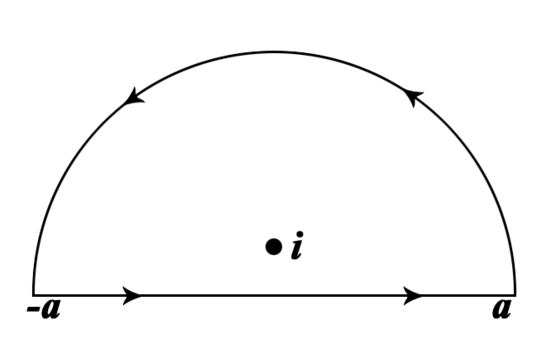
\includegraphics[scale=0.7]{contour}
	\caption{Wikipedia}
\end{figure}
in order to avoid integrating over some pole $z = i$.

\subsubsection{Cauchy Integral Formula}
In order to the perform the integral above in general, we can make use of something called the \textit{Cauchy integral formula}, which goes as follows. For any analytic function $f(z)$, if $z_0$ is interior to the contour $C$ then we have
\begin{align}
\boxed{f(z_0) = \f{1}{2\pi i}\int_C \f{f(z)}{z - z_0}\,dz}
\end{align}

which says that the values of $f$ inside the contour $C$ such that $\abs{z} = 2$ is determined by the value of $f$ on $C$. Let's use this to actually perform the integral. For example, say we would like to compute 
\begin{align}
\int_C \f{z\,dz}{(9-z^2)(z+i)} 
\end{align}
along a contour $C$ that contains only the \textit{pole} $z_0 = -i$. Then we first re-write the integral to match the Cauchy integral formula:
\begin{align}
\int_C \f{z\,dz}{(9-z^2)(z+i)} &= \int_C \f{1}{z+i}\lp \f{z}{9 - z^2} \rp\,dz
\end{align}
where $f(z)$ here is
\begin{align}
f(z) = \f{z}{9 - z^2}
\end{align}
which is analytic for $\abs{z} \leq 2$. By the integral formula, we have that
\begin{align}
\int_C \f{1}{z+i}\lp \f{z}{9 - z^2} \rp\,dz = f(z_0 = -i) = 2\pi i f(-i) = 2\pi i \f{-i}{9 + 1} = \f{\pi}{5}.
\end{align}

So believe it or not, we've just evaluated the integral without doing any integration!












\subsubsection{Taylor \& Laurent series}

Complex functions can have Taylor series or Laurent series, which is like Taylor series in a way except the powers are negative. 

\begin{figure}[!htb]
	\centering
	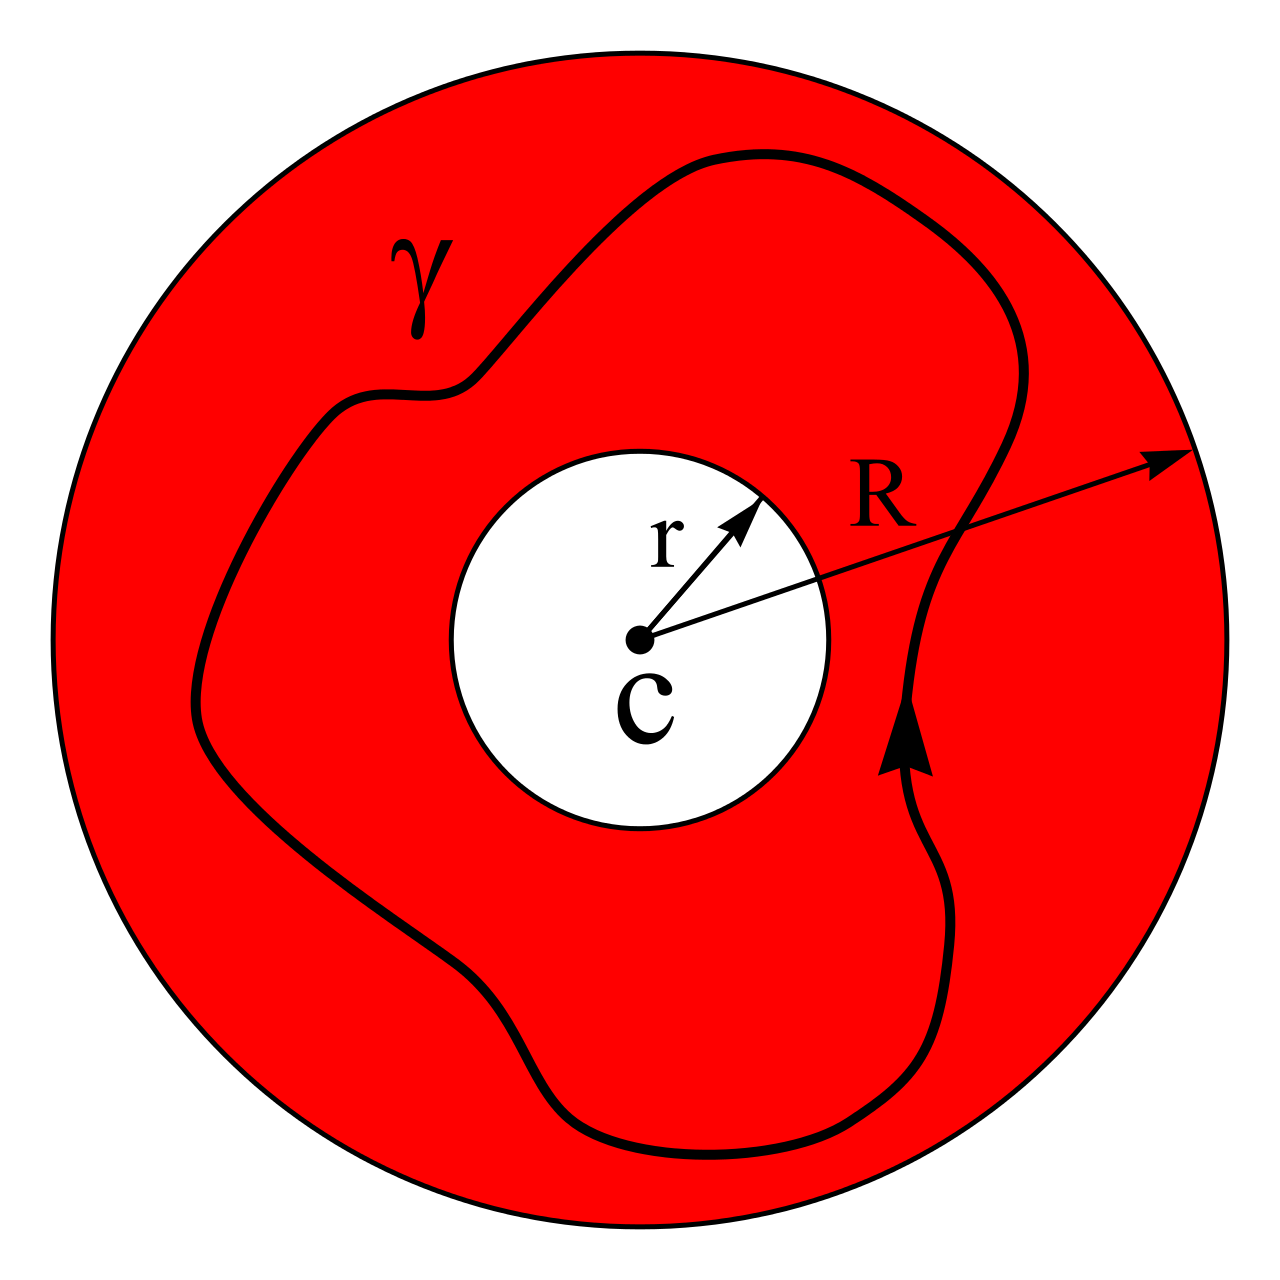
\includegraphics[scale=0.15]{laurent}
	\caption{Wikipedia}
\end{figure}

Let the contours $C_1$ and $C_2$ be concentric circles centered on $z_0$ with radii $r_1$ and $r_2$ where $r_2 < r_1$. Then we have a theorem which says if $f$ is analytic on $C_1$ and $C_2$ and everywhere in between then at each point $z$ in-between or on $C_1$ or $C_2$, we have
\begin{align}
\boxed{f(z) = \sum^\infty_{n=0}a_n (z - z_0)^n + \sum^\infty_{n=0}\f{b_n}{(z- z_0)^n}}
\end{align}
where
\begin{align}
a_n &= \f{1}{2\pi i }\int_{C_1} \f{f(s)\,ds}{(s - z_0)^{n+1}}\hspace{0.5cm} n = 0,1,2,3,\dots \\ 
b_n &= \f{1}{2\pi i }\int_{C_2} \f{f(s)\,ds}{(s - z_0)^{-n+1}}\hspace{0.5cm} n = 1,2,3,\dots
\end{align}
The series defined above is called the \textit{Laurent series} for $f$. \\

One thing we can do to recover a ``single'' contour $C$ is shrinking the inner radius $r_2 \to 0$, so that the domain becomes a punctured neighborhood of radius $r_1$ around $z_0$: $0 < \abs{z - z_0} < r_1$ and the $b_n$'s vanish.\\

If $f$ is analytic at all points inside and on $C_1$ then $f(z) / (z - z_0)^{-n+1}$ is also analytic since $-n+1 \leq 0$ and $b_n = 0$. This means the series reduces to a Taylor series. 











\subsubsection{The Residue Theorem}

A singular point of a function $f(z)$ is a point $z_0$ where $f$ is not analytic at $z_0$ but is analytic at every point in some neighborhood of $z_0$. So for example, the function $f(z) = 1/z$ is analytic everywhere except at $z=0$, so $z=0$ is a singular point. \\

Isolated singularities have neighborhoods around them on which $f$ is analytic. \\

When $f$ has an isolated singular point $z_0$, we define the \textit{residue} of $f$ at $z_0$ is the coefficient $b_1$ of its Laurent series:
\begin{align}
\boxed{b_1 = \f{1}{2\pi i}\int_{C} f(z)\,dz}
\end{align}

Note that the residue $b_1$ is the coefficient in the $1 / (z - z_0)$ term in the Laurent series:
\begin{align}
f(z) = \f{b_1}{z - z_0} + \dots
\end{align}


\textbf{The Residue Theorem:} Let $f$ be an analytic function in and on a closed contour $C$ except where it has singular points $z_1, z_2, \dots$ with corresponding residues $b_1, b_2, \dots$. Then 
\begin{align}
\boxed{\int_C f(z)\,dz = 2\pi i (b_1 + b_2 + \dots)}
\end{align}
i.e., the contour integral of $f$ around some contour $C$ which contains some of the singular points of $f$ is $2\pi i$ times the sum of the corresponding residues. \qed


For example, let's say we want to evaluate
\begin{align}
\int_C \f{5z - z}{z(z- 1)}\,dz
\end{align}
where the contour $C$ contains both the $0$ and $1$ poles. Then we first write the integrand so that it matches has the form of a Laurent series:
\begin{align}
\f{5z - 2}{z(z- 1)} = \f{1}{z}\lp \f{5z - 2}{z - 1} \rp = \f{1}{z-1}\lp\f{5z - 2}{z}\rp.
\end{align}
We find that the for the $z_0 = 0$ pole the residue is 
\begin{align}
b_1 = \f{0-2}{0-1} = 2.
\end{align}
For the $z_1 = 1$ pole the residue is
\begin{align}
b_2 = \f{5 - 2}{1} = 3.
\end{align}
So by the residue theorem,
\begin{align}
\int_C \f{5z - z}{z(z- 1)}\,dz = 2\pi i(2+3) = 10\pi i.
\end{align}


Let's do another example to get more comfortable. Suppose we want to evaluate
\begin{align}
\int_C \f{z^2}{1+z}\,dz
\end{align}
for a contour $C$ that contains the pole $z = -1$. For this pole, the corresponding residue is $(-1)^2 = 1$, so 
\begin{align}
\int_C \f{z^2}{1+z}\,dz = 2\pi i(1) = 2\pi i.
\end{align}

There are certainly techniques to evaluate integrals involving much more complicated poles, but we won't worry about that for now. 














\subsubsection{Evaluating real improper integrals}



One of many very nice applications of the residue theorem and the contour integrals is evaluating real improper integrals. Consider a general real improper integral 
\begin{align}
\int^{\infty}_{-\infty}f(x)\,dx
\end{align}
where $f$ now is a function that takes on real-valued arguments. If we extend $f$ over the complex plane and $f(z)$ has a pole at $z_0$ with positive imaginary part, then consider the contour with $\abs{z_0} < R$ which looks like the following
\begin{figure}
	\centering
	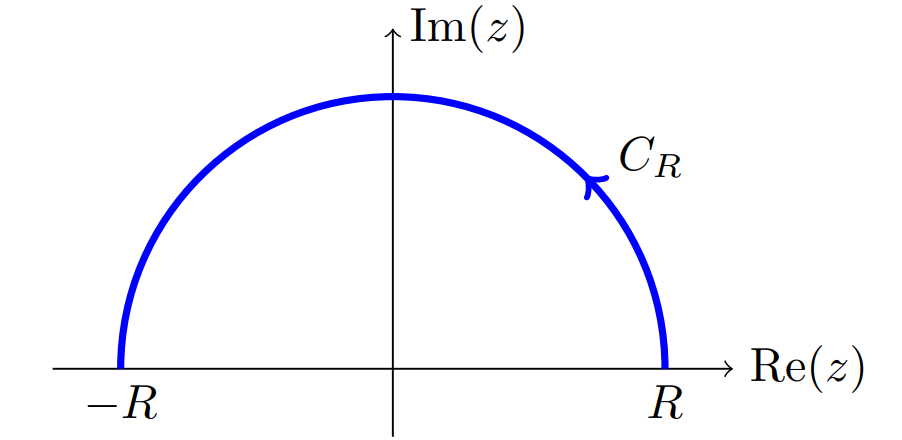
\includegraphics[scale=0.7]{improper}
\end{figure}
If 
\begin{align}
f(z) = \f{g(z)}{z - z_0}
\end{align}
then we have from the theorems
\begin{align}
\oint_C f(z)\,dz = 2\pi i g(z_0).
\end{align}
But we can also extend and make the contour very large by taking $R\to \infty$ since the contour integral stays the same
\begin{align}
\oint_C f(z)\,dz = \lim_{R\to \infty}\lp \int^R_{-R}f(x)\,dx + \int_{C_R}f(z)\,dz\rp
\end{align}
where the first term on the RHS is exactly the real improper integral we're looking for. Thus, so long as $f(z)$ on $C_R$ vanishes when we take $R\to \infty$, we must have that
\begin{align}
\boxed{\int^{\infty}_{-\infty}f(x)\,dx = 2\pi i g(z_0)}
\end{align}\qed



For example, let's say we want to evaluate the following integral
\begin{align}
\int^\infty_{-\infty} \f{2x^2 - 1}{x^4 + 5x^2 + 4}\,dx.
\end{align}

Well, while we can certainly try to do this completely on the real line, we can avoid the singularities by doing the contour integral. So let's write the integrand as
\begin{align}
f(z) = \f{2x^2 - 1}{(z^2 + 1)(z^2 + 4)}
\end{align}
which has poles at $z = \pm i, \pm 2i$. We also observe that for large $z$, $\abs{f(z)}\to 0$. This allows us to do use the contour integral. If we pick a contour that looks like a half-circle in the upper half plane with the base being the real axis, so that its radius is bigger than 2 (so that we can extend the contour to infinity), then we have, by what we've shown earlier
\begin{align}
\int_C f(z)\,dz = \int^\infty_{-\infty}f(x)\,dx + 0
\end{align}
where $0$ simply denotes the piece that vanishes when $R \to \infty$. With this, we move on to evaluating the contour integral. But notice that the contour includes only the $i$ and $2i$ poles, so we will only have two residues. Because we only have the $i$ and $2i$ poles, we write
\begin{align}
f(z) = \f{1}{z-i}\f{2z^2 - 1}{(z+i)(z^2 + 4)} = \f{1}{z - 2i}\f{2z^2 - 1}{(z^2 + 1)(z - 2i)}.
\end{align}
The residue that $z = i$ is then $i/2$, while the residue that $z = 2i$ is $-3i/4$. So the improper integral is
\begin{align}
\int^\infty_{-\infty} \f{2x^2 - 1}{x^4 + 5x^2 + 4}\,dx = 2\pi i\lp \f{i}{2} - \f{3i}{4} \rp = \f{\pi}{2}.
\end{align}










\newpage




\subsection{Multi-valued Functions \& Branch Cuts}



























\newpage




\subsection{From Field to Particle to Force}

Now that we've had the mathematical machinery in hand, we can tackle our worries about the $1/(k^2 - m^2)$ the keeps popping up in the integrals. \\

Let's start slow and try to evaluate the following integral
\begin{align}
\int^\infty_{-\infty} \f{dk}{k^2 - m^2}.
\end{align}

We obviously see that there are two poles $k =-m$ and $k = m$. While we will try to evaluate this using the a contour integral, it's not clear how we'll start because the poles are on the real axis. To resolve this slight issue, we will ``tilt'' the complex plane so that the ``poles'' are no longer on the real axis. \\

What we'll do is letting $m^2 \to m^2 - i\epsilon$ where $\epsilon > 0$ is some arbitrarily small positive number, just so we could push the pole a bit away from the real axis. Our goal is to evaluate the contour integral with $m^2 - i\epsilon$, then take the limit as $\epsilon\to \infty$ and hopefully get something finite. So, with $m^2 \to m^2 - i\epsilon$, we have
\begin{align}
k^2 - m^2 &\to k^2 - (m^2 - i\epsilon) \\ 
&= (k - \sqrt{m^2 - i\epsilon})(k + \sqrt{m^2 - i\epsilon}). 
\end{align}
Since $\epsilon$ can be chosen to be arbitrarily small, we will just do an expansion on the square root term without worrying to much
\begin{align}
\sqrt{m^2 - i\epsilon} &= m\sqrt{1 - \f{i\epsilon}{m^2}} \\ 
&\approx m - \f{i\epsilon}{2m} \\ 
&= m - i\epsilon' 
&\equiv m - i\epsilon
\end{align}
where we have let $\epsilon$ become the $\epsilon'$, which is something we can do because again $\epsilon$ can be chosen to be arbitrarily small. With this, we have
\begin{align}
k^2 - (m^2 - i\epsilon) = (k - (m - i\epsilon))(k + (m - i\epsilon)).
\end{align}

So now we have two poles at $k = m-i\epsilon$ and $k = -m + i\epsilon$, which are off the real axis. The next thing to do now is to evaluate the contour integral. We can make a closed contour using either the upper half-plane half-circle, or the lower half-plane half circle, each enclosing a different pole. 

\begin{figure}[!htb]
	\centering
	\includegraphics*[scale=0.1]{poles}
	\caption{Sketch by Prof. Robert Bluhm}
\end{figure}

Consider the contour integral on the left hand side. The enclosed pole here is $k = m - i\epsilon$. So to compute the residue we write
\begin{align}
\f{1}{k^2 - m^2 + i\epsilon} = \f{1}{k - (m - i\epsilon)}\f{1}{k + (m - i\epsilon)}.
\end{align}
The residue is therefore
\begin{align}
\f{1}{(m - i\epsilon) + (m - i\epsilon)} \to \f{1}{2m}
\end{align}
as we take $\epsilon \to 0$. If we consider the other contour then the residue is going to take on a minus sign, $-1/2m$. However, worry not, because the integrals over the real line in two contours have opposite directions. This means in either case, we get
\begin{align}
\int^\infty_{-\infty}\f{dk}{k^2 - m^2 + i\epsilon} = 2\pi i \lp \f{-1}{2m} \rp = \boxed{\f{-i\pi}{m}}.
\end{align}
Note that we can use the residue theorem to evaluate the integral here because as $k\to \infty, 1/(k^2 - m^2 + i\epsilon) \to 0$.

Okay, now suppose we want to evaluate something that is closer to what we're dealing with earlier:
\begin{align}
\int^\infty_{-\infty} \f{dk\, e^{ik(x-y)}}{k^2 - m^2 + i\epsilon}.
\end{align}

Consider the same two contours. We will see that both contours don't always work in both cases and whether the contour you choose works depends on whether $(x-y)$ is positive or negative. \\

Suppose $x - y > 0$. Then on $C_R$, we have that
\begin{align}
e^{iz(x-y)} \sim e^{i(iR)(x-y)} = e^{-R(x-y)} \to 0 \text{ as } R\to \infty,
\end{align}
where $iR$ represents the argument (up to phase shifts) that is fed into the exponent when integrating over the contour. On the other contour, however, because the argument now looks like $-iR$ times a phase factor, the sign of the exponent becomes positive, which means the function blows up. So, we see that the contour on the lower half-plane doesn't work when $x - y > 0$. The opposite happens when we have $x - y < 0$: only the contour on the lower half-plane works. \\

With this and the fact that the integrand still goes to zero as $k\to \infty$, we have for $x - y > 0$,
\begin{align}
\int^\infty_{-\infty} \f{dk\, e^{ik(x-y)}}{k^2 -m^2 + i\epsilon} = \int_C \f{dz \, e^{iz(x-y)}}{z^2 - m^2 + i\epsilon}.
\end{align}

So depending on the sign at $(x-y)$, we get combinations to the residue 
\begin{align}
\f{e^{2mi(x-y)}}{2m} \text{ or } \f{e^{-2mi(x-y)}}{-2m}
\end{align}
when $x - y>0$ and $x-y < 0$, respectively. \\

With this, we can now tackle the free theory propagator in QFT, which is given by
\begin{align}
\D(x-y) = \int \f{d^4 k }{(2\pi)^4} \f{e^{ik(x-y)}}{k^2 - m^2 + i\epsilon}
\end{align}

Here
\begin{align}
k^2 &= k_0^2 - \vec{k}^2 \\ 
d^4k &= dk_0\,d^3k
\end{align}
where we're using the conventional Minkowskian metric $\eta_{\mu\nu} = \text{diag}(1,-1,-1,-1)$. With this we rewrite the integral as
\begin{align}
\D(x-y) &= \f{1}{(2\pi)^4} \int^\infty_{-\infty}dk_0\,\int^\infty_{-\infty}d^3k\f{e^{ik_0(x^0 - y^0)}e^{-i\vec{k}\cdot(\vec{x} - \vec{y})}}{k_0^2 - (\vec{k}^2 + m^2) + i\epsilon},
\end{align}
where we don't really have to worry too much about $k^0$ or $k_0$ because of the metric. Now we'll call
\begin{align}
w_k^2 = \vec{k}^2 + m^2,
\end{align}
which the equivalent to the total energy. For the $k_0$ integration, which is an integration over time:
\begin{align}
k_0^2 - w_k^2 + i\epsilon = (k_0 - (w_k - i\epsilon))(k_0 + (w_k -i\epsilon))
\end{align}
and so we have poles at $k_0 = w_k - i\epsilon$ and $-w_k + i\epsilon$.\\

Once again, to perform this integral (correctly), we must pick the correct half-plane to close the contour. This choice depends on $x_0 - y_0$, which is the \textbf{time-ordering}. \\

It turns out that for $x^0 - y^0 >0$, we use the upper contour of radius $R$, where we have 
\begin{align}
e^{ik_0(x-y)} \sim e^{i(iR)(x^0-y^0)} = e^{-R(x^0-y^0)} \sim 0.
\end{align}
In this case, the pole is at $k_0 = -w_k + i\epsilon$. And so we can now evaluate the integral over all \textit{space} in the expression above:
\begin{align}
&\f{1}{(2\pi)^4}\int^\infty_{-\infty}d^3k\f{e^{ik_0(x^0 - y^0)}e^{-i\vec{k}\cdot(\vec{x} - \vec{y})}}{k_0^2 - (\vec{k}^2 + m^2) + i\epsilon}\\
= &\int \f{1}{k_0 + (w_k - i\epsilon)} \lp 
\f{d^3k}{(2\pi)^4}\f{e^{ik_0(x^0 - y^0)} e^{-i\vec{k}\cdot(\vec{x} - \vec{y})}}{k_0 - (w_k - i\epsilon)}
\rp.
\end{align}
Now, remember that this is our $f(k_0)$, and what we're actually trying to evaluate here is 
\begin{align}
\D(x-y) = \int dk^0 f(k_0).
\end{align}
By writing $f(k_0)$ as the triple integral over all \textit{space} like above, the residue is given by
\begin{align}
\int\f{d^3k}{(2\pi)^4}\f{e^{ik_0(x^0 - y^0)} e^{-i\vec{k}\cdot(\vec{x} - \vec{y})}}{k_0 - (w_k - i\epsilon)}
\end{align}
evaluated at the pole $k_0 = -w_k + i\epsilon$, taking $\epsilon \to 0$. The value of this at $k_0 = -w_k +i\epsilon$ as $\epsilon\to 0$ is
\begin{align}
&\int \f{d^3k}{(2\pi)^4} \f{e^{-iw_k(x^0 - y^0)}e^{-i\vec{k}\cdot (\vec{x} - \vec{y})}}{-w_k - w_k} \\ 
= &\int \f{d^3k}{(2\pi)^4} \f{e^{-iw_k(x^0 - y^0)}e^{-i\vec{k}\cdot (\vec{x} - \vec{y})}}{-2w_k}.
\end{align}
This is the residue. And so the value of the propagator is then
\begin{align}
\D(x-y) = \int dk^0 \,f(k_0) = 2\pi i \lb \int \f{d^3k}{(2\pi)^4} \f{e^{-iw_k(x^0 - y^0)}e^{-i\vec{k}\cdot (\vec{x} - \vec{y})}}{-2w_k} \rb. 
\end{align}
So,
\begin{align}
\D(x-y) = \f{1}{(2\pi)^3} \int \f{-i}{2w_k}d^3k\,e^{-i[w_k(x^0 - y^0) + \vec{k}\cdot(\vec{x} - \vec{y})]}
\end{align}

On the other hand, if $x^0 - y^0 <0$, then we would use the other pole and close the contour in the lower half-plane to get
\begin{align}
\D(x-y) &= -2\pi i\f{1}{(2\pi)^4}\int d^3k\, \f{e^{iw_k(x^0 - y^0)}e^{-i\vec{k}\cdot(\vec{x} - \vec{y})}}{2w_k} \\ 
&= \f{1}{(2\pi)^3}\int  \f{-i}{2w_k} d^3k\,e^{iw_k(x^0 - y^0)}e^{-i\vec{k}\cdot(\vec{x} - \vec{y})}  \\
&= \boxed{\f{1}{(2\pi)^3}\int \f{-i}{2w_k}d^3k\,e^{i[w_k(x^0 - y^0) - \vec{k}\cdot(\vec{x} - \vec{y})]}}
\end{align}
where the minus sign comes from integrating over the real line in the $(-)$ direction. The pole is now $k_0 = w_k - i\epsilon$ and the residue is
\begin{align}
\f{1}{(2\pi)^3}\int d^3k\, \f{e^{iw_k(x^0 - y^0)}e^{-i\vec{k}\cdot(\vec{x} - \vec{y})}}{2w_k}
\end{align}
when $\epsilon \to 0$.\\

We see that the expression for the propagator when $x^0 - y^0 > 0$ and $x^0 - y^0 < 0$ differ by a little bit in the sign of $\vec{k}$ in the factor inside the exponent. However, we note that because of symmetry, by letting $\vec{k} \to -\vec{k}$ in the $x^0 - y^0 > 0$ case and using symmetry:
\begin{align}
\int d^3k = \int d^3(-\vec{k})
\end{align}
we can re-write:
\begin{align}
{\D(x-y) = \f{1}{(2\pi)^3} \int \f{-i}{2w_k}d^3k\,e^{-i[w_k(x^0 - y^0) - \vec{k}\cdot(\vec{x} - \vec{y})]}}
\end{align} 
for the $x^0 - y^0 > 0$ case. \\

The next thing we want to do is combining the two propagators into a single expression. This requires having a function that specifies the correct sign of $x^0 - y^0$, which is exactly what the Heaviside step function does. Define
\begin{align}
\theta = \begin{cases}
1 \hspace{0.5cm} x^0 - y^0 > 0\\ 
0 \hspace{0.5cm} x^0 - y^0 < 0
\end{cases}
\end{align}
where we will take $\theta = 1/2$ if $x^0 = y^0$.\\


With this and taking $y = 0$ to be the initial spacetime and $x^0 = t$,  we can write the propagator as
\begin{align}\label{propag}
\boxed{\D(x) = \f{-i}{(2\pi)^3}\int \f{d^3k}{ 2 w_k} \lb e^{-i[w_kt - \vec{k}\cdot\vec{x}]}\theta(t) + e^{i[w_kt - \vec{k}\cdot\vec{x} ]}\theta(-t)\rb}
\end{align}

Let us note a few things here before moving on. For spacelike $x$, i.e., $x = (t,\vec{x}) = (t,0)$, we have that if $t >0$ (in the future cone), the propagator has the form
\begin{align}
\D(x) = \f{-i}{(2\pi)^3}\int \f{d^3k}{2 w_k}e^{-iw_kt}.
\end{align}
This says the propagator is a superposition of plane waves and oscillates. Similar with the past cone where $t<0$, $\D$ also oscillates but with a different phase ($e^{iw_kt}$). \\

For timelike $x$, i.e., $x = (0,\vec{x})$, we have that 
\begin{align}
\D(x) = \f{-i}{(2\pi)^3}\int \f{d^3k}{ 2 w_k}e^{-i\vec{k}\cdot\vec{x}} =\f{-i}{(2\pi)^3}\int \f{d^3k}{ 2 \sqrt{\vec{k}^2 + m^2}}e^{-i\vec{k}\cdot\vec{x}} .
\end{align}
where we have flipped the sign of $\vec{k}$ again to cancel the factor of $1/2$. \textit{In order to evaluate this integral, we will need to understand \textbf{branch cuts}, which we will cover later. }






































\newpage





\subsection{From field to particle}

Recall that from free scalar with source $J(x)$ we have obtained a functional $W(J)$:
\begin{align}
W(J) = -\f{1}{2}\iint d^4xd^4y\, J(x)\D(x-y)J(y)
\end{align}
where $W(J)$ is called the generating function for connected diagrams, and $\D(x-y)$ is basically the Green's function which carries the effects of the source at $y$ to $x$. \\


In terms of the Fourier transform 
\begin{align}
J(x) &\equiv  \F^{-1}[J(k)](x) = \int d^4x \, J(k)e^{-ikx}\\
\D(x-y) &\equiv \f{1}{(2\pi)^4}\int d^4k\,\f{1}{k^2 - m^2}e^{ik(x-y)}
\end{align}
So we have
\begin{align}
W(J) = -\f{1}{2}\f{1}{(2\pi)^4}\int d^4k\, J(k)^* \f{1}{k^2 - m^2 + i\epsilon}J(k) 
\end{align}
where we have taken the complex conjugate of $J(x)$ to get the correct Fourier transform.  \\

Now, consider the case where we have two sources $J_1, J_2$ in spacetime such that $J(x) = J_1(x) + J_2(x)$
\begin{figure}[!htb]
	\centering
	\includegraphics*[scale=0.7]{source}
	\caption{From Zee}
\end{figure}
Then $W(J)$ contains four terms involving $J_1$ and $J_2$. One of the terms contains $J_2^* J_1$:
\begin{align}
W(J) = -\f{1}{2}\int \f{d^4k}{(2\pi)^4} J_2^*(k)\f{1}{k^2 - m^2 + i\epsilon} J_1(k).
\end{align} 

We interpret this as follows: in region 1 in spacetime there is a source that sends out some disturbance in the field, which is then absorbed by a sink in region 2 in spacetime. \\

When $k^2 = m^2$, $k$ is said to be on mass shell. For arbitrary $k$, it is a linguistic convenience to say that a``virtual particle'' of momentum $k$ propagates from
the source to the sink.











\subsubsection{Particle to force}


Consider the same source $J = J_1 + J_2$ again and consider the $W(J)$, neglecting the $J_1^*J_1$ and $J_2^*J_2$ self-interactions. And suppose that 
\begin{align}
J_a(\vec{x}) = \delta^{(3)}(\vec{x} - \vec{x}_a).
\end{align}
Note that $J$ is real and so we will get a factor of $2$ when obtaining $W(J)$. \\

Plugging everything into 
\begin{align}
W(J) = -\f{1}{2}\iint d^4xd^4y\, J(x)\D(x-y)J(y).
\end{align}
we obtain (remember the factor of 2...)
\begin{align}
W(J) &= -\f{2}{2}\iint dx^0 dy^0 \int \f{d^0k}{2\pi} e^{ik^0(x-y)^0} \int \f{d^3k }{(2\pi)^3} \f{e^{i\vec{k}\cdot (\vec{x}_1 - \vec{x}_2)}}{k^2 - m^2 + i\epsilon}\\
&= -\iint dx^0 dy^0 \int \f{d^0k}{2\pi} e^{ik^0(x-y)^0} \int \f{d^3k }{(2\pi)^3} \f{e^{i\vec{k}\cdot (\vec{x}_1 - \vec{x}_2)}}{k^2 - m^2 + i\epsilon}
\end{align}
where the piece
\begin{align}
2\int \f{d^0k}{2\pi} e^{ik^0(x-y)^0}
\end{align}
comes from the transforms of the source delta functions and the piece
\begin{align}
\f{e^{i\vec{k}\cdot (\vec{x}_1 - \vec{x}_2)}}{k^2 - m^2 + i\epsilon} \\
\end{align} 
comes from the transform of the propagator $\D(x-y)$. \\

Next, integrating over all $y^0$ and absorbing the delta-function-transform piece give us a delta function, which sets $k^0$ to zero. As a result,
\begin{align}
k^2 = k^0 - \vec{k}^2 = \vec{k}^2
\end{align}
So that $W(J)$ becomes
\begin{align}
W(J) = \lp \int dx^0 \rp \int \f{d^3x}{(2\pi)^3} \f{e^{i\vec{k}\cdot (\vec{x}_1 - \vec{x}_2)}}{\vec{k}^2 + m^2}
\end{align}
where we have dropped $i\epsilon$ because the denominator is can no longer be zero.   \\

Next, recall the \textbf{generating function} we have defined previously
\begin{align}
\mathcal{Z} = \zeta e^{iW(J)} \sim \bra{0}e^{-iHT}\ket{0} = e^{-iET}
\end{align} 
where
\begin{align}
T = \int dx^0
\end{align}
is the time interval. So we have 
\begin{align}
\boxed{E = -\int \f{d^3k}{(2\pi)^3}\f{e^{i\vec{k}\cdot(\vec{x}_1 - \vec{x}_2)}}{\vec{k}^2 + m^2}}
\end{align}
Let us evaluate this integral. First, we write 
\begin{align}
\vec{x} &= \vec{x}_1 - \vec{x}_2 \\ 
u &\equiv \cos\theta = (\vec{k},\vec{x}).
\end{align}
In spherical coordinates where
\begin{align}
k &= \abs{\vec{k}} \\
r &= \abs{\vec{x}},
\end{align}
we have the volume element is
\begin{align}
d^3k = k^2 \sin \theta \,dk,d\theta\,d\phi = -  k^2 \, d(\cos\theta)\,d\phi.
\end{align}
But notice that even though we get an extra minus sign, the integration bounds also flips accordingly, so the overall sign of the integral doesn't chance. Thus,
\begin{align}
E &= -\int \f{d^3k}{(2\pi)^3}\f{e^{i\vec{k}\cdot(\vec{x}_1 - \vec{x}_2)}}{\vec{k}^2 + m^2} \nonumber\\
&= -\f{1}{(2\pi)^3}\int_0^{2\pi}d\phi\,\int^\infty_0 dk\,k^2 \int^{1}_{-1}d(\cos\theta)\f{e^{ikx\cos\theta}}{k^2 + m^2} \nonumber\\
&= -\f{1}{(2\pi)^2}\int^\infty_0 dk\,k^2 \int^{1}_{-1}du\,\f{e^{ikru}}{k^2 + m^2} \nonumber\\
&= -\f{1}{(2\pi)^2} \int^\infty_0 dk\,\f{1}{k^2 + m^2} \lp \f{1}{ikr}e^{ikru} \rp\bigg\vert^1_{-1}\nonumber\\
&= -\f{1}{(2\pi)^2} \int^\infty_0 dk\,\f{1}{k^2 + m^2} \lb \f{2i}{ikr}\sin(kr)\rb\nonumber\\
&= -\f{2i}{(2\pi)^2ir} \int^\infty_0 dk\,\f{k\sin (kr)}{k^2 + m^2}\nonumber\\
&= -\f{1}{(2\pi)^2r} \int^\infty_{-\infty}dk\,\f{k\sin (kr)}{k^2 + m^2} \hspace{0.5cm} \text{(even integrand)}\nonumber\\
&= -\f{1}{(2\pi)^2r} \int^\infty_{-\infty}dk\,\lp\f{1}{k - im}\rp\f{k\sin(kr)}{k + im}\nonumber\\
&= -\f{1}{(2\pi)^2r}\int^\infty_{-\infty}dk\,\lp\f{1}{k - im}\rp\f{1}{2i}\f{k(e^{ikr} - e^{-ikr})}{k + im} \nonumber\\
&= -\f{1}{(2\pi)^2r}\int^\infty_{-\infty}dk\,\lp\f{1}{k - im}\rp\f{1}{2i}\f{k(e^{ikr} + e^{ikr})}{k + im}\nonumber\\
&=  -\f{1}{(2\pi)^2r}\int^\infty_{-\infty}dk\,\lp\f{1}{k - im}\rp\f{1}{i}\f{k e^{ikr}}{k + im}\nonumber\\
&= -\f{1}{(2\pi)^2ri}\int^\infty_{-\infty}dk\,\lp\f{1}{k - im}\rp\f{k e^{ikr}}{k + im}\nonumber \\
&= -\f{1}{(2\pi)^2ri}\int_{C}dk\,\lp\f{1}{k - im}\rp\f{k e^{ikr}}{k + im} \hspace{0.5cm} \text{*contour around } im \nonumber\\
&= -\f{1}{(2\pi)^2ri}(2\pi i)\f{im e^{i(+im)r}}{im + im} \nonumber\\
&= \boxed{-\f{1}{4\pi r}e^{-mr}}
\end{align}

Thus the energy is \textbf{negative}, which means the two delta function sources give an attractive force. We identify $E$ as the potential energy between two static sources. We also note the range of the attractive force generated by the field $\psi$ is determined inversely by the mass $m$ of the particle. Does this sound familiar?????















\subsubsection{The Origin of Force}

We now see that the exchange of particle (via $\D$) can produce a force, which is given by the potential. We can associate a particle with each of the known forces: photon with the electromagnetic force, graviton with gravity(?). \\

More importantly, however, we see where the \textbf{inverse square law} comes from, based on the form of the potential. We notice that if the force-carrying particle has mass 0 (which is the case for photon in electromagnetism and graviton in gravitation) then the potential energy has the form
\begin{align}
E = \f{1}{4\pi r}.
\end{align}
The gradient of this gives the force, which is proportional to $1/r^2$. \\

Where does this come from? The answer can be traced all the way back to the Lagrangian density for the simplest field theory where we have $\p_\mu$ and $\p^\mu$, i.e., two powers of the spacetime derivative. This ensures Lorentz invariance. 












\subsubsection{Connected versus disconnected}

We might want to represent the integrand
\begin{align}
J(x)\D(x-y)J(y)
\end{align}
as a connected path in $W(J)$ to present a disturbance from $y$ to $x$. This is the beginning of Feynman diagrams. 
\begin{figure}[!htb]
	\centering
	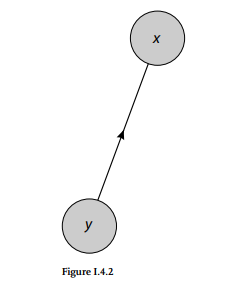
\includegraphics[scale=0.7]{feynman-1}
	\caption{From Zee}
\end{figure}

Next, recall the definition of the generation function $\mathcal{Z}$:
\begin{align}
\boxed{\mathcal{Z}(J) = \mathcal{Z}(0)e^{iW(J)} = \mathcal{Z}(J=0)\sum^\infty_{n=0}\f{[iW(J)]^n}{n!}}
\end{align}
The $n=2$ term is given by
\begin{align}
\f{1}{2!}\lp -\f{i}{2} \rp^2 \iiiint d^4x_1d^4x_2d^4x_3d^4x_4\D(x_1 - x_2)\D(x_3 - x_4)J(x_1)J(x_2)J(x_3)J(x_4).
\end{align}
The integrand is given by
\begin{figure}[!htb]
	\centering
	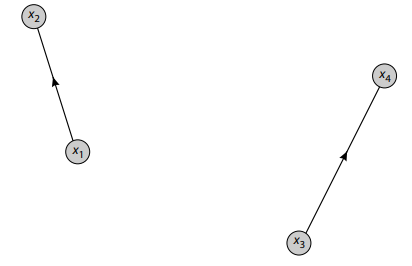
\includegraphics[scale=0.6]{feynman-2}
	\caption{From Zee}
\end{figure}
We see this is the correct figure because the $1\to 2$ propagation is independent of $3\to 4$. 




















\subsubsection{Like charges repel}

Quantum field theory of electromagnetism is called quantum electrodynamics, or QED for short. For this section we will consider the theory of a massive spin 1 vector. We will assume that the photon mass is nonzero, only to plug in $m=0$ in the end to see if things are okay. \\

Recall the Lagrangian:
\begin{align}
\lag = -\f{1}{4}F_{\mu\nu}F^{\mu\nu}
\end{align}
where
\begin{align}
F_{\mu\nu} = \p_\mu A_\nu - \p_\nu A_\mu
\end{align}
where $A_\mu(x)$ is the vector potential. With our assumption that the mass of the photon is nonzero, we will introduce both a mass term and a source term to the Lagrangian, which then becomes
\begin{align}
\lag = -\f{1}{4}F_{\mu\nu}F^{\mu\nu} + \f{1}{2}m^2A_\mu A^\mu + A_\mu J^\mu.
\end{align}
Note that the source here is a just a current, which satisfied the conservation law:
\begin{align}
\p_\mu J^\mu = 0.
\end{align}
The path integral of this theory is
\begin{align}
\Z = \int \mathfrak{D} \,Ae^{iS[A]} = e^{iW(J)}
\end{align}
where the functional action in terms of the vector potential
\begin{align}
S[A] = \int d^4x\,\lag &= \int d^4x \lb -\f{1}{4}F_{\mu\nu}F^{\mu\nu} + \f{1}{2}m^2A_\mu A^\mu + A_\mu J^\mu \rb \\ 
&= \int d^4x\,\lb \f{1}{2}A_\mu \lb (\p^2 + m^2)g^{\mu\nu} - \p^\mu \p^\nu \rb A_\nu + A_\mu J^\mu  \rb
\end{align}
where the second equality comes from integration by parts. Now, just like when we were dealing with the free scalar field with source, we want the propagator $\D$ to be the inverse of the differential operator, i.e.,
\begin{align}
\lb (\p^2 + m^2)g^{\mu\nu} - \p^\mu \p^\nu \rb \D_{\nu\lambda}(x) = \delta^\mu_\lambda \delta^{(4)}(x).
\end{align}
Just like before, by going into momentum space we can extract the wave vector $k$ from the differential operator. To do this, we will have to go way back to the beginning of this section, Fourier transform everything and putting everything back into a original equation. The propagator in position space is related to the propagator in momentum space by
\begin{align}
\D{\nu\lambda}(x) = \F[\D(k)](x) = \int \f{d^4k}{(2\pi)^4} D_{\nu\lambda}(k)e^{ik(x)}.
\end{align}
Plugging this back into our equation and writing the delta function as a Fourier transform to get
\begin{align}
\int \f{d^4k}{(2\pi)^4}D_{\nu\lambda}(k) \lb (\p^2 + m^2)g^{\mu\nu} - \p^\mu \p^\nu \rb e^{ikx} = \delta^\mu_\lambda \int \f{d^4k}{(2\pi)^4}e^{ikx}.
\end{align}
Letting the differential operator act on $e^{ikx}$
\begin{align}
\int \f{d^4k}{(2\pi)^4}D_{\nu\lambda}(k) \lb -(k^2 - m^2)g^{\mu\nu} + k^\mu k^\nu \rb e^{ikx} = \delta^\mu_\lambda \int \f{d^4k}{(2\pi)^4}e^{ik(x)}.
\end{align}
And so it must follow that
\begin{align}
\lb -(k^2 - m^2)g^{\mu\nu} + k^\mu k^\nu \rb \D_{\nu\lambda}(k) = \delta^{\mu}_\lambda
\end{align}
Solving for the propagator, we get
\begin{align}
\boxed{D_{\nu\lambda}(k) = \f{-g_{\nu\lambda} + k_\nu k_\lambda / m^2}{k^2 - m^2}}
\end{align}
This is the \textbf{masive vector meson propagator}, or the photon propagator loosely speaking. With this, we can now write the generating function for connected diagrams as
\begin{align}
W(J) = -\f{1}{2}\int \f{d^4k}{(2\pi)^4}J^\mu(k)^*\f{-g_{\nu\lambda} + k_\nu k_\lambda / m^2}{k^2 - m^2 + i\epsilon} J^\nu(k)
\end{align}
where the $i\epsilon$ is added to the denominator because (as you can tell this is coming) we will need to do a contour integral around a pole to get a finite answer. \\

We also have that the conservative of current $\p_\mu J^\mu = 0$ in momentum space becomes $k_\mu J^\mu = 0$, this means the $k_\mu k_\nu$ term in the numerator gets killed by the $J's$. We also have that $g_{\mu\nu} \sim 1$, so effectively the generating function is 
\begin{align}
W(J) \sim \f{1}{2}\int \f{d^4k}{(2\pi)^4}J^\mu(k)^*\f{1}{k^2 - m^2 + i\epsilon} J^\nu(k)
\end{align}
where the minus sign disappears. So, by comparing this result to what we have found in the previous section, we see that the energy obtained is positive so long as the charge densities $J$'s have the same sign. This basically says like charges repel. \\

With this, no more computation is needed. With
\begin{align}
E = \f{1}{4\pi r}e^{-mr},
\end{align} 
we simply let the photon mass go to zero to get
\begin{align}
E \to \f{1}{4\pi r}.
\end{align}
This is exactly the form of the electric potential in electrostatics.







\subsubsection{Planck Mass}

The Planck Mass, denoted $M_{Pl}$ is defined in terms of the Newton's law of gravity:
\begin{align}
V(r) = \f{G_N m_1 m_2}{r} = \f{m_1 m_1}{M^2_{Pl}} \lp \f{1}{r}\rp.
\end{align}
Numerically, 
\begin{align}
M_{Pl} \approx 10^{19} \text{ GeV}.
\end{align}
It is clear why gravity is so weak compared to, say, the electromagnetic force. 







\newpage


\subsection{Feynman Diagrams}







\subsubsection{Gaussian Integrals and their Moments}


Before getting into how trying to evaluate these integrals gives us Feynman diagrams, we should quickly revisit Gaussian integrals, as they are \textit{very} similar to many integrals in QFT.\\

The first basic result is the following:
\begin{align}
I = \int_\mathbb{R}dx\, e^{-x^2} = \sqrt{\pi}.
\end{align}
A very clever way to do this is to move to the two dimensional case and try to evaluate
\begin{align}
I^2 = \int_{\mathbb{R}^2} dxdy\, e^{-x^2 - y^2}.
\end{align}
We can move into polar coordinates and do a change of variables to get
\begin{align}
I^2 = \int_0^\infty (2\pi) rdr\,e^{-r^2}.
\end{align}
We can evaluate this integral with a $u$-substitution. to get
\begin{align}
I^2 = 2\pi \f{1}{2} = \pi \implies I = \sqrt{\pi}.
\end{align}
In general,
\begin{align}
\boxed{\int_\mathbb{R} dx\, \exp\lp -\f{a}{2}x^2 + bx \rp = \sqrt{\f{2\pi}{a}} \exp\lp \f{b^2}{2a} \rp }
\end{align}
We do this by completing the square then rescaling and shifting the integration variables. (This is why we have a left over exponent in the end.)\\

The next things we want to evaluate are various moments of the Gaussian, i.e., integrals like
\begin{align}
I_n = \int_\mathbb{R} dx\, x^n \exp\lp -\f{a}{2}x^2 \rp.
\end{align}
We assume that $n$ is a positive integer. If $n$ is odd then the integrand is an odd function, so when it is integrated over a symmetric domain we get 0. On the other hand, when $n$ is even, we use Feynman's \textbf{differentiating-under-the-integral-sign} trick. Here is how it works:\\


\textbf{Feynman's integration technique:} Consider the previous integral:
\begin{align}
\int_\mathbb{R} dx\, \exp\lp -\f{a}{2}x^2 + bx \rp.
\end{align}  
We notice that when we take the derivative of the integrand with respect to $b$ we bring down a factor of $x$:
\begin{align}
\f{d}{db}\, \exp\lp -\f{a}{2}x^2 + bx \rp = x\exp\lp -\f{a}{2}x^2 + bx \rp.
\end{align}
So, in order to get $x^n$ in the integrand of the integral
\begin{align}
I_n = \int_\mathbb{R} dx\, x^n \exp\lp -\f{a}{2}x^2 \rp,
\end{align}
we will take $\p_b$ of the other integrand $n$ times to bring down $x^n$ then set $b = 0$. Let's do this:
\begin{align}
\lp\f{d}{db}\rp^n \exp\lp -\f{a}{2}x^2 + bx \rp \bigg\vert_{b=0} = x^n \exp\lp -\f{a}{2}x^2 + bx \rp\bigg\vert_{b=0} = x^n \exp\lp -\f{a}{2}x^2\rp,
\end{align}
which is exactly what we wanted. Okay, but we still haven't successfully evaluated the integral yet. To do this, we will look at the original ``guiding'' equation again:
\begin{align}
\int_\mathbb{R} dx\, \exp\lp -\f{a}{2}x^2 + bx \rp = \sqrt{\f{2\pi}{a}} \exp\lp \f{b^2}{2a} \rp.
\end{align}
Differentiate wrt $b$ $n$ times and setting $b = 0$ in the end gives
\begin{align}
\lp\f{d}{db}\rp^n \int_\mathbb{R} dx\, \exp\lp -\f{a}{2}x^2 + bx \rp \bigg\vert_{b=0} 
&= \sqrt{\f{2\pi}{a}}\lp\f{d}{db}\rp^n \exp\lp \f{b^2}{2a} \rp\bigg\vert_{b=0} \nonumber \\
\int_\mathbb{R}\lp\f{d}{db}\rp^n  dx\, \exp\lp -\f{a}{2}x^2 + bx \rp\bigg\vert_{b=0} 
&= \sqrt{\f{2\pi}{a}}\lp\f{d}{db}\rp^n \exp\lp \f{b^2}{2a} \rp\bigg\vert_{b=0}.
\end{align}
Therefore,
\begin{align}
\boxed{\int_\mathbb{R}dx\, x^n \exp\lp -\f{a}{2}x^2\rp 
= \sqrt{\f{2\pi}{a}}\f{n!}{(n/2)!(2a)^{n/2}}}
\end{align}
Note that $n$ here is even. If $n$ is odd then the integral is zero. Next, to correctly normalize these integrals, we can find the normalization factor simply by
\begin{align}
\boxed{\f{\int_\mathbb{R}dx\, x^n \exp\lp -\f{a}{2}x^2\rp }{\int_\mathbb{R}dx\, \exp\lp -\f{a}{2}x^2\rp } = \f{n!}{(n/2)!(2a)^{n/2}}}
\end{align}
These higher moments of the Gaussian are called the \textbf{correlation functions}. 	 \\

So how are these higher moments related to Feynman diagrams? The answer is given by the combinatoric interpretation of values of the integrals. Suppose we would like make ($n/2$) pairs from $n$ distinguishable things. The answer is 
\begin{align}
{ n \choose n}{n-2 \choose 2}\dots {2 \choose 2} \times \f{1}{(n/2)!} = \f{n!}{2^{n/2}(n/2)!}.
\end{align}
This is not so different from what we just found, except the factor of $1/a$. This is where the physics come in. Observe that if we add in a weight factor of $1/a$ each time we make a pair then we get the same thing from the integral. These factors of $1/a$ are the \textbf{propagators}! 









\subsubsection{Anharmonicity in field theory}

So far, integrals in free field theory have been Gaussian, meaning we can evaluate them one way or the other using the prescription laid out above. However, particles don't interact in this theory because we don't have ``anharmonic'' in the Lagrangian (these make the equation of motion no longer linear). \\

Revisit the combinator interpretation of the values of the integrals above. If we associate to each pair of the $n$ things an \textit{edge} connecting them, then we see when things are alreay in pairs they don't interact with our future choices. This is quite hand-wavy, but the idea is that if the exponent inside the integrand is quadratic (or can be square-completed) then we can evaluate things exactly. But what if there are higher order terms, or alternatively \textit{anharmonic} terms? \\

Suppose we add only one anharmonic term $-(\lambda / 4!)\phi^4$ to our free field theory and try to evaluate
\begin{align}
\Z(J) = \int \mathfrak{D}\phi \exp\lp i\int d^4x\,  \f{1}{2}\lb(\p \phi)^2 - m^2 \phi^2 \rb - \f{\lambda}{4!}\phi^4 + J(x)\phi \rp.
\end{align}
This isn't so doable anymore! It's possible, but imagine adding higher order terms to the Lagrangian! 











\subsubsection{Feynman diagrams: A baby problem}

Let us try to evaluate a simpler version of the integral above:
\begin{align}
\Z(J) = \int^\infty_{-\infty} dq\, \exp\lp -\f{1}{2}m^2 q^2 - \f{\lambda}{4!}q^4 + Jq \rp.
\end{align}

Here we don't have a nice trick to complete the square. However, we can use the exact result obtained earlier with the higher order moments of the Gaussian integral to try to approximate this integral. The idea is to Taylor expand the higher order term and turn it into a polynomial in $q^4$ when appropriate:
\begin{align}
\exp\lp -\f{1}{2!}\f{\lambda}{4!}q^4 \rp = 1 - \lp\f{\lambda}{4!}\rp q^4 + \f{1}{2!}\lp\f{\lambda}{4!}\rp^2 q^8 - \dots
\end{align}
With this, we get
\begin{align}
\Z(J) = \int^\infty_{-\infty} dq\,  \lb 1 - \lp\f{\lambda}{4!}\rp q^4 + \f{1}{2!}\lp\f{\lambda}{4!}\rp^2 q^8 - \dots \rb e^{ -\f{1}{2}m^2 q^2 + Jq }.
\end{align}

Then, we \textit{simply} integrate term-by term. This we can do because now they are just $q^{4n}$ moments of the original Gaussian, i.e., each term has the form
\begin{align}
\int_\mathbb{R} dq\, e^{(-1/2)m^2 q^2 + Jq}q^{4n}.
\end{align}
To bring down a factor of $q^{4n}$ for each term we have to differentiate wrt $J$ $4n$ times:
\begin{align}
\int_\mathbb{R} dq\, e^{(-1/2)m^2 q^2 + Jq}q^{4n} &= \int_\mathbb{R}\,dq \lp \f{d}{dJ} \rp^{4n} e^{(-1/2)m^2 q^2 + Jq} \\
&=   \lp \f{d}{dJ} \rp^{4n} \int_\mathbb{R}dq \, e^{(-1/2)m^2 q^2 + Jq}.
\end{align}

Because $\Z(J)$ is a sum of such terms, we get
\begin{align}
\boxed{\Z(J) = \lb 1 - \lp\f{\lambda}{4!}\rp \f{d^4}{dJ^4} + \f{1}{2!}\lp\f{\lambda}{4!}\rp^2 \f{d^8}{dJ^8} - \dots \rb\int_\mathbb{R}dq \, e^{(-1/2)m^2 q^2 + Jq}}
\end{align}

But that's not all, observe that we have just replaced 
\begin{align}
q^{4n} \to \f{d^{4n}}{dJ^{4n}}.
\end{align}

So it only makes sense that we write 
\begin{align}
\exp\lb -\f{\lambda}{4!}\lp \f{d}{dJ} \rp^4 \rb = \lb 1 - \lp\f{\lambda}{4!}\rp \f{d^4}{dJ^4} + \f{1}{2!}\lp\f{\lambda}{4!}\rp^2 \f{d^8}{dJ^8} - \dots \rb.
\end{align}
We also know how to evaluate the leftover integral by completing the squares. So, 
\begin{align}
\int_\mathbb{R}dq \, e^{(-1/2)m^2 q^2 + Jq} = \sqrt{\f{2\pi}{m^2}}\exp\lp \f{J^2}{2m^2} \rp.
\end{align}

Thus we have successfully evaluated $\Z(J)$:
\begin{align}
\boxed{\Z(J) = \exp\lb -\f{\lambda}{4!}\lp \f{d}{dJ} \rp^4 \rb \sqrt{\f{2\pi}{m^2}}\exp\lp \f{J^2}{2m^2} \rp = \sqrt{\f{2\pi}{m^2}} e^{-\f{\lambda}{4!}\lp \f{d}{dJ} \rp^4} e^\f{J^2}{2m^2}}
\end{align}

From now on, we will let 
\begin{align}
\Z(J=0, \lambda =0) = \sqrt{2\pi / m^2} \equiv \Z(0,0)
\end{align}
We will also define
\begin{align}
\boxed{\tilde{\Z} = \f{\Z(J)}{\Z(J = 0, \lambda = 0) } = e^{-\f{\lambda}{4!}\lp \f{d}{dJ} \rp^4} e^\f{J^2}{2m^2}}
\end{align}



\subsubsection{From Integrals to Feynman diagrams}


Recall from the previous section that
\begin{align}
\tilde{\Z}(J) =  e^{-\f{\lambda}{4!}\lp \f{d}{dJ} \rp^4} \times e^\f{J^2}{2m^2}.
\end{align}
By expanding the two exponential we can obtain \textit{any term} in a double series expansion of $\Z(J)$ in $\lambda$ and in $J$:
\begin{align}
\tilde{\Z}(J) = \lb 1 - \lp\f{\lambda}{4!}\rp \f{d^4}{dJ^4} + \f{1}{2!}\lp\f{\lambda}{4!}\rp^2 \f{d^8}{dJ^8} - \dots \rb \lb 1 + \f{J^2}{2m^2} + \f{1}{2!}\lp \f{J^2}{2m^2} \rp^2 + \dots \rb
\end{align}
Why do we want to this? Because each Feynman diagram can be associated with a term of certain orders in $\lambda$ and in $J^4$. Let's do a few examples.\\

\textbf{Find the term with $\lambda$ and $J^4$:} We first notice that all of the powers of $\lambda$'s come from the first exponential. So if we want $\lambda^1$, we pick
\begin{align}
- \lp\f{\lambda}{4!}\rp \f{d^4}{dJ^4} 
\end{align}
from the first exponential. Then, because we want to be left over with $J^4$ after $d^4/dJ^4$ acts on the $J^{4n}$ term from the second exponential, we pick the $J^8$ term from the exponential, namely
\begin{align}
\f{1}{4!}\lp \f{J^2}{2m^2} \rp^4.
\end{align}
So the term with $\lambda^1$ and $J^4$ is 
\begin{align}
- \lp\f{\lambda}{4!}\rp \f{d^4}{dJ^4} \f{1}{4!}\lp \f{J^2}{2m^2} \rp^4 &= -\lp\f{\lambda}{4!}\rp \lp\f{1}{4!}\rp \lp \f{1}{2m^2} \rp^4 \f{d^4}{dJ^4}J^8\\
&=  -\lp\f{\lambda}{4!}\rp \lp\f{1}{4!}\rp \lp \f{1}{2m^2}\rp \lp\f{8!}{4!}\rp J^4\\
&= \boxed{(-\lambda)\lb\f{8!}{(4!)^3 (2m^2)^4}\rb J^4}
\end{align}\qed


\textbf{Find the term with $\lambda^2$ and $J^4$:} Since we want $\lambda^2$, we must pick from the first exponential the term
\begin{align}
\f{1}{2!}\lp \f{\lambda}{4!} \rp^2\lp \f{d^4}{dJ^4} \rp^2.
\end{align}
Since we want $J^4$ in the end, we must pick a $J^{12}$ in the second exponential, which is
\begin{align}
\f{1}{6!}\lp \f{J^2}{2m^2} \rp^6.
\end{align}
So the desired term is 
\begin{align}
\f{1}{2!}\lp \f{\lambda}{4!} \rp^2\lp \f{d^4}{dJ^4} \rp^2 \f{1}{6!}\lp \f{J^2}{2m^2} \rp^6 &= \lambda^2 \f{1}{2!(4!)^2 6! (2m^2)^6}\f{12!}{4!}J^4 \\
&= \boxed{\lambda^2 \f{12!}{2! (4!)^3 6! (2m^2)^6 } J^4 }
\end{align}\qed


\textbf{Find the term with $\lambda^2$ and $J^6$:} Let us do this last example before getting some insights into the patterns here. Since we want $\lambda^2$, we pick from the first exponential
\begin{align}
\f{1}{2!}\lp \f{\lambda}{4!} \rp^2\lp \f{d^4}{dJ^4} \rp^2.
\end{align}
Since we want to be left with $J^6$, we want to start with $J^{6+8} = J^{14}$ in the second exponential
\begin{align}
\f{1}{7!}\lp \f{J^2}{2m^2} \rp^7.
\end{align}
So the desired term is 
\begin{align}
\f{1}{2!}\lp \f{\lambda}{4!} \rp^2  \lp \f{d^4}{dJ^4} \rp^2  \f{1}{7!}\lp \f{J^2}{2m^2} \rp^7 &= \lambda^2 \f{1}{2!(4!)^2 7! (2m^2)^7}\f{14!}{6!}J^6 \\
&= \boxed{\lambda^2 \f{14!}{2! (4!)^2 6! 7! (2m^2)^7 } J^6 }
\end{align}\qed


\textbf{What is the general pattern here?} Let the picking and simplifying sink in a bit, we get the following pattern. Suppose we want a term with $\lambda^l$ and $J^{j}$ where $j$ must be even otherwise there is no such $J^j$ term. Then we first want the $\lambda^l$ term in the first exponent, which means we want
\begin{align}
\f{1}{l!}\lp\f{\lambda}{4!}\rp^l \lp\f{d^4}{dJ^4}\rp^l.
\end{align}
With this, we next want to be left with a $J^j$, so we need the $(4l + j)^\text{th}$ power of $J$ in the second exponential. So we take
\begin{align}
\f{1}{[(4l + j)/2]!}\lp \f{J^2}{2m^2} \rp^\f{4l + j}{2}.
\end{align}
So the desired term is 
\begin{align}
&\,\,\,\f{1}{l!}\lp\f{\lambda}{4!}\rp^l \lp\f{d^4}{dJ^4}\rp^l \f{1}{(4l + j)!}\lp \f{J^2}{2m^2} \rp^\f{4l + j}{2} \\
=&\,\,\,\f{1}{l!(4!)^l [(4l+j)/2]! (2m^2)^{(4l+j)/2}} \lambda^l  \lp\f{d^4}{dJ^4}\rp^l J^{4l + j} \\ 
= &\,\,\, \boxed{\f{(4l + j)!}{l!\,(4!)^l\, j!\, [(4l+j)/2]!\,     (2m^2)^{(4l+j)/2}} \,\lambda^l \, J^j}
\end{align}\qed



Now, the more practice we have the better we get at doing this. It's not a surprise we slowly see a pattern. We observe that we can associate a diagram with each term and codify some \textbf{rules}, which are follow:
\begin{enumerate}
	\item Diagrams are made of lines and vertices at which 4 lines meet (because $J^4$ is the principal factor)
	\item For each vertex assign a factor of $(-\lambda)$
	\item For each line assign $1/m^2$. Note: this goes back to the combinatoric interpretation.
	\item For each external end assign $J$.
\end{enumerate}\qed


Let's go through some examples again:\\


\textit{Diagrams for $(1/m^2)^4 \lambda J^4$:} We notice that because there is only 1 $\lambda$ term, so we can only have 1 vertex (a vertex is defined as where four lines meet). We also have only 4 externals ends, because we have $J^4$. We should also have only 4 lines because we have $(1/m^2)^4$. So the following diagrams satisfy these conditions:\\

\begin{figure}[!htb]
	\centering
	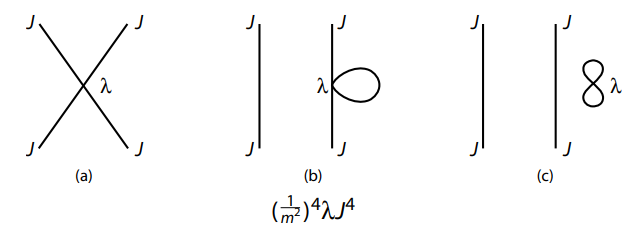
\includegraphics[scale=0.7]{feynman-diagram-1}
	\caption{From Zee}
\end{figure}\qed


\textit{Diagrams for $\sim (-\lambda)^2 J^4 / (m^2)^6$:} We expect to get 2 vertices, 4 external ends, and 6 lines. The following diagrams satisfy these conditions:\\

\begin{figure}[!htb]
	\centering
	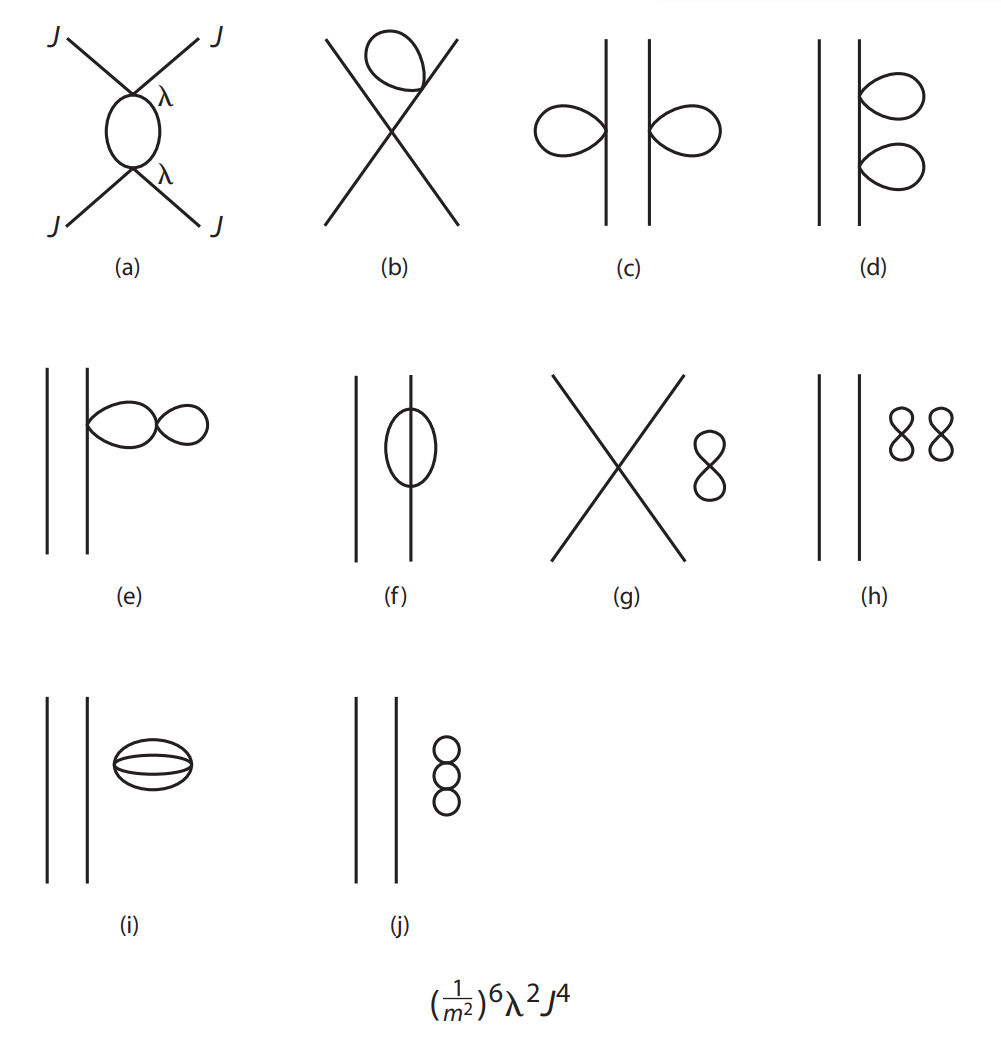
\includegraphics[scale=0.3]{feynman-diagram-2}
	\caption{From Zee}
\end{figure} \qed


\textit{Diagrams for $\sim (-\lambda)^2 J^6 / (m^2)^7$:} We expect to get 2 vertices, 6 external ends, and 7 lines. The following diagrams satisfy these conditions:\\

\begin{figure}[!htb]
	\centering
	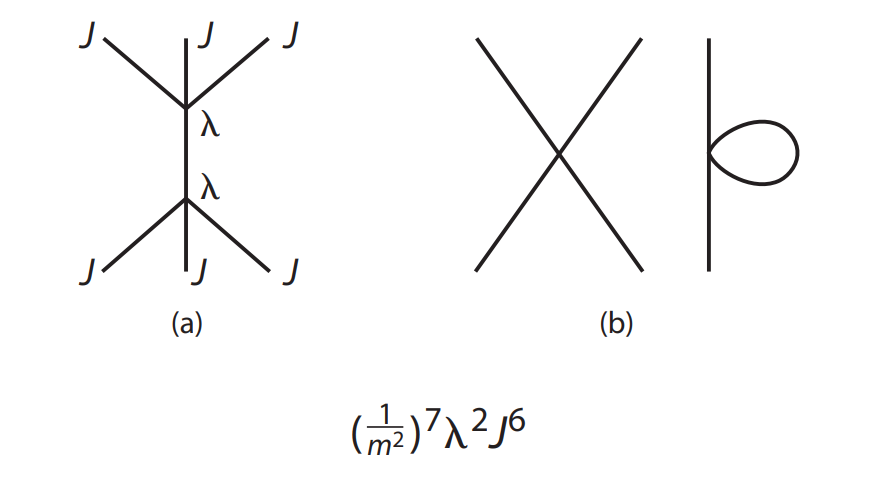
\includegraphics[scale=0.4]{feynman-diagram-3}
	\caption{From Zee}
\end{figure} \qed

Of course, we have seen that if we want a term with $\lambda^l$ and $J^j$ (where $j$ is even), i.e., $l$ vertices and $j$ external ends, then we have $(4l + j)$ lines.







\subsubsection{Another approach: Wick contraction}

Recall that in the baby problem we evaluated this integral
\begin{align}
\Z(J) = \int^\infty_{-\infty} dq\, \exp\lp -\f{1}{2}m^2 q^2 - \f{\lambda}{4!}q^4 + Jq \rp
\end{align}
by doing a power expansion in the $e^{\sim \lambda}$ term:
\begin{align}
\exp\lp -\f{1}{2!}\f{\lambda}{4!}q^4 \rp = 1 - \lp\f{\lambda}{4!}\rp q^4 + \f{1}{2!}\lp\f{\lambda}{4!}\rp^2 q^8 - \dots
\end{align}


If please, we can also re-do this problem starting out with a power expansion in $J$:
\begin{align}
\exp\lp Jq \rp = \sum^\infty_{s=0} \f{J^s q^s}{s!}.
\end{align}
With this, we can write and define the $G^{(s)}$ coefficients as
\begin{align}
\boxed{\Z(J) = \sum^\infty_{s=0} \f{J^s}{s!}\int_\mathbb{R}dq\, q^s \exp\lp -\f{1}{2}m^2 q^2 - \f{\lambda}{4!}q^4 \rp \equiv \Z(0,0) \sum^\infty_{s=0} \f{J^s}{s!} G^{(s)} }
\end{align}
These $G^{(6)}$ coefficients are analogues of Green's functions in field theory. \\

To evaluate the integral from here, we sort of repeat what we did earlier, except now we expand and differentiate under the integral sign with respect to $\lambda$. The coefficients $G^{(s)}$ can then be evaluated by the Wick contraction. We won't go into much detail about this for now. 












\subsubsection{Connected vs. Disconnected}

Looking at a few Feynman diagrams generated by our baby problem, we can see that some of them are connected while some aren't. For example, diagram $(a)$ for the $(1/m^2)^4\lambda J^4$ is connected, while $(b)$ and $(c)$ aren't. \\


Recall our definition of the generating function
\begin{align}
\Z(J, \lambda) = \Z(J=0, \lambda)e^{W(J,\lambda)} = \Z(J=0, \lambda)\sum^\infty_{N=0}\f{[W(J,\lambda)]^N}{N!}.
\end{align}



By definition the term $\Z(J=0, \lambda)$ consists of diagrams with no external source $J$. These diagrams look like loops such as Figure \ref{fig:loops}.

\begin{figure}[!htb]
	\centering
	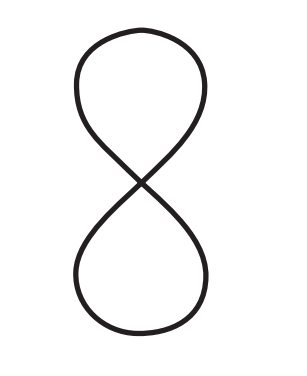
\includegraphics[scale=0.5]{feynman-diagram-4}
	\caption{From Zee}
	\label{fig:loops}
\end{figure}

So we see that while $W(J)$ is a sum of only connected diagrams, $\Z$ contains both types of diagrams, connected and disconnected. This is why $\Z$ is called the generating function, and $W$ is called the generating function for connected diagrams. 













\subsubsection{A child problem: Integrals, Wick contraction \& Propagation}


Before graduating to full field theory, let us try a slightly more difficult problem where we want to evaluate the following multiple integral
\begin{align}
\boxed{\Z(J) = \int_{\mathbb{R}^N} \prod_i^N dq_i \exp\lp -\f{1}{2}q^\top A q - \f{\lambda}{4!}q^4 + J\cdot q  \rp}
\end{align}
where
\begin{align}
q^4 = \sum_i q_i^4.
\end{align}
Notice that this an $N-$dimensional problem, and so $q$ are now vectors in some $N-$dimensional space, and $A$ is some matrix. We will assume that $A$ plays the role of some kind metric, which means it is positive definite and symmetric. In statistics, $A$ is the covariance matrix. In physics, $A$ can carry information about \textit{the} metric. \\

Recall our previous result:
\begin{align}
\Z(J)  = \sqrt{\f{2\pi}{m^2}} e^{-\f{\lambda}{4!}\lp \f{d}{dJ} \rp^4} e^\f{J^2}{2m^2}
\end{align}
starting from 
\begin{align}
\Z(J) = \int^\infty_{-\infty} dq\, \exp\lp -\f{1}{2}m^2 q^2 - \f{\lambda}{4!}q^4 + Jq \rp.
\end{align}


How do we generalize our result from the baby problem to this one in higher dimensions? To do this, we must first try an easier $n-$dimensional ``Gaussian integral'' such as
\begin{align}
I = \int \prod_i^N dx_i\, \exp\lp -\f{1}{2}x^\top A x \rp
\end{align}
where $A$ is again an positive definite and symmetric matrix (i.e., metric). We will first diagonalize $A$ with an orthogonal matrix $M$:
\begin{align}
D = MAM^{-1} = \text{diag}(\lambda_1, \lambda_2, \dots, \lambda_N)
\end{align}
where $\lambda_i$ are the eigenvalues of $A$. With this, 
\begin{align}
\det(A) = \det(D) = \prod_i^N \lambda_i
\end{align}The goal of doing this is so that we can ``de-couple'' the $x$'s in the exponent, by which we can bring the product sign outside of the integral. Once the product sign is outside of the integral, we will simply be left with a product of 1-dimensional Gaussian integrals. \\

We will also let
\begin{align}
z = M^\top x = (x^\top M)^\top.
\end{align}
The Jacobian of this change of basis is just the identity because $\det(M) = 1$, so we have
\begin{align}
I 
&= \int \prod_i^N dz_i\, \exp\lp -\f{1}{2}z^\top D z \rp \\ 
&= \prod_i^N \underbrace{\int dz_i\, \exp\lp -\f{1}{2}\lambda_i z_i^2\rp}_{\sqrt{2\pi / \lambda_i}} \hspace{0.5cm} D\text{ is diagonal}\\ 
&= \prod_i^N \sqrt{\f{2\pi}{  \lambda_i}}\\
&= \boxed{\sqrt{\f{(2\pi)^N}{\det(A)}}} \hspace{0.5cm}\text{since } \det(A) = \prod_i^N \lambda_i.
\end{align}

Nice! What if we added a source term? 
\begin{align}
I_J = \int \prod_i^N dx_i\, \exp\lp -\f{1}{2}x^\top A x + J^\top x \rp
\end{align}


Let $x = y + A^{-1}J$, then because $A = A^\top$, we must have that
\begin{align}
-\f{1}{2}x^\top A x + J^\top x &= -\f{1}{2}(y + A^{-1}J)^\top A (y + A^{-1}J) + J^\top (y + A^{-1}J)\nonumber\\
&= -\f{1}{2}\lb y^\top A y +2J^\top y + J^\top A^{-1}AA^{-1}J\rb + J^\top y + JA^{-1}J \nonumber\\
&= -\f{1}{2}y^\top A y + \f{1}{2}J^\top A^{-1}J.
\end{align}
Thus,
\begin{align}
I_J &= \int \prod_i^N dx_i\, \exp\lp -\f{1}{2}y^\top A y + \f{1}{2}J^\top A^{-1}J \rp\\
&= \exp\lp \f{1}{2}J^\top A^{-1}J \rp \int \prod_i^N dx_i\, \exp\lp -\f{1}{2}y^\top A y \rp \\
&= \boxed{ \sqrt{\f{(2\pi)^N}{\det(A)}} \exp\lp \f{1}{2}J^\top A^{-1}J \rp}
\end{align}

Let us now look back to the child problem. What we just did here with $n-$dimensional Gaussian integrals suggests expanding in $\lambda$ inside the integral first:
\begin{align}
\Z(J) &= \int_{\mathbb{R}^N} \prod_i^N dq_i  \exp\lp -\f{1}{2}q^\top A q - \f{\lambda}{4!}q^4 + J^\top q  \rp \nonumber \\ 
&= \int_{\mathbb{R}^N} \prod_i^N dq_i  \exp\lp -\f{1}{2}q^\top A q + J^\top q \rp
\lc \sum_{j=0}^\infty   \f{\lb -\f{\lambda}{4!}q^4\rb^j}{j!}  \rc \nonumber \\
&= \int_{\mathbb{R}^N} \prod_i^N dq_i  \exp\lp -\f{1}{2}q^\top A q + J^\top q \rp
\lc 1 -\f{\lambda}{4!}q^4 + \f{1}{2!}\lp-\f{\lambda}{4!}q^4\rp^2 + \dots   \rc  
\end{align}

To evaluate this integral, we integrate term-by-term, using the Feynman's differentiating under the integral sign. But we have first be very careful here because we're dealing with vectors. Recall that
\begin{align}
q^4 = \sum_i q_i^4.
\end{align}
Every factor of $\p / \p J_{i}$ brings down a factor of $q_i$. So, in order to get any $q^4$ term, we need
\begin{align}
\sum_i \lp\f{\p}{\p J_i}\rp^4.
\end{align}
Thus 
\begin{align}
\exp\lp \f{-\lambda q^4}{4!} \rp \sim \exp\lb \f{-\lambda }{4!} \lp\sum_i \f{\p }{\p J_i} \rp^4\rb.
\end{align}
Therefore, from integrating term-by-term by differentiating under the integral sign, then adding the terms up together we get that
\begin{align}
\Z(J) &= \lc 1 + \lb\f{-\lambda}{4!} \lp\sum_i \f{\p }{\p J_i} \rp^4\rb + \f{1}{2!}\lb\f{-\lambda }{4!} \lp\sum_i \f{\p }{\p J_i} \rp^4\rb^2 + \dots   \rc \nonumber \\
&\,\,\,\,\,\hspace{1cm}\times\int_{\mathbb{R}^N} \prod_i^N dq_i  \exp\lp -\f{1}{2}q^\top A q + J^\top q \rp \nonumber\\
&= \exp\lb \f{-\lambda q^4}{4!} \lp\sum_i \f{\p }{\p J_i} \rp^4\rb \times \lb  \int_{\mathbb{R}^N} \prod_i^N dq_i  \exp\lp -\f{1}{2}q^\top A q + J^\top q \rp\rb \nonumber\\
&= \sqrt{\f{(2\pi)^N}{\det(A)}}\exp\lb \f{-\lambda q^4}{4!} \lp\sum_i \f{\p }{\p J_i} \rp^4\rb  \exp\lb \f{1}{2}J^\top A^{-1}J \rb,
\end{align}
where we of course have just evaluated the last integral by a change of variables. With this result, we can write more compactly
\begin{align}
\boxed{\Z(J) =  \sqrt{\f{(2\pi)^N}{\det(A)}}\, e^{-(\lambda/4!) \sum_i (\p/\p J_i)^4} \, e^{\f{1}{2}J^\top A^{-1} J}}
\end{align}




Alternatively, we can first expand in powers of $J$ first, before in powers of $\lambda$. Let's start with the expansion in $J$:
\begin{align}
\Z(J) &= \int_{\mathbb{R}^N} \prod_i^N dq_i  \exp\lp -\f{1}{2}q^\top A q - \f{\lambda}{4!}q^4 + J^\top q  \rp \nonumber \\ 
&= \int_{\mathbb{R}^N} \prod_i^N dq_i  \exp\lp -\f{1}{2}q^\top A q - \f{\lambda}{4!}q^4 \rp \lc \sum^\infty_{s=0} \f{(J^\top q)^s}{s!}  \rc \nonumber \\ 
&= \int_{\mathbb{R}^N} \prod_i^N dq_i  \exp\lp -\f{1}{2}q^\top A q - \f{\lambda}{4!}q^4 \rp \lc \sum^\infty_{s=0} \f{\lb \sum_{l_s}^N (J_{l_s} q_{l_s}) \rb^s}{s!}  \rc \nonumber \\ 
&= \sum^\infty_{s=0} \sum^N_{l_1 = 1}\dots \sum^N_{l_s = 1} \f{1}{s!}J_{l_1}\dots J_{l_s} \int_{\mathbb{R}^N} \lp\prod_i^N dq_i \rp \exp\lp -\f{1}{2}q^\top A q - \f{\lambda}{4!}q^4 \rp q_{l_1}\dots q_{l_s}\nonumber\\
&\equiv \boxed{\Z(0,0) \sum^\infty_{s=0} \sum^N_{l_1 = 1}\dots \sum^N_{l_s = 1} \f{1}{s!}J_{l_1}\dots J_{l_s} G^{(s)}_{l_1 \dots l_s}}
\end{align}
where we defined the Green's function coefficients such that
\begin{align}
\boxed{\Z(0,0) G^{(s)}_{l_1 \dots l_s} \equiv \int_{\mathbb{R}^N} \lp\prod_i^N dq_i \rp \exp\lp -\f{1}{2}q^\top A q - \f{\lambda}{4!}q^4 \rp q_{l_1}\dots q_{l_s}}
\end{align}


One main difference between the child problem and the baby problem is that the Green's function coefficients in the child problem have indices. What this means is that we have \textit{propagation from here to there}. Also, notice that these coefficients with an \textbf{odd} number of indices are \textbf{zero}, since the integrand in these cases are odd functions. \\

To see what these $G$ coefficients are we should try to evaluate a few illuminating examples. Let us start with the ``2-point Green's function'' to zeroth order in $\lambda$. The strategy to evaluate this integral is to put back a $J$ into the exponent and differentiate in order to get the $q$ terms in the integrand, then set $J=0$. We note that every factor of $\p / \p J_{l_s}$ gives a factor of $q_{l_s}$. Let's proceed:
\begin{align}
G^{(2)}_{l_1l_2}(\lambda = 0) &= \f{1}{\Z(0,0)}\int_{\mathbb{R}^N} \lp\prod_i^N dq_i \rp \exp\lp -\f{1}{2}q^\top A q  \rp q_{l_1}q_{l_2} \nonumber \\ 
&= \f{1}{\Z(0,0)}\int_{\mathbb{R}^N} \lp\prod_i^N dq_i \rp \exp\lp -\f{1}{2}q^\top A q  + J^\top q  \rp q_{l_1}q_{l_2}\bigg\vert_{J=0}\nonumber\\
&= \f{1}{\Z(0,0)}\int_{\mathbb{R}^N} \lp\prod_i^N dq_i \rp \f{\p}{\p J_{l_1}} \f{\p}{\p J_{l_2}} \exp\lp -\f{1}{2}q^\top A q  + J^\top q  \rp \bigg\vert_{J=0}\nonumber\\
&= \underbrace{\f{1}{\Z(0,0)}}\f{\p}{\p J_{l_1}} \f{\p}{\p J_{l_2}} \underbrace{ \int_{\mathbb{R}^N} \lp\prod_i^N dq_i \rp  \exp\lp -\f{1}{2}q^\top A q  + J^\top q  \rp} \bigg\vert_{J=0}\nonumber\\
&= \lp \sqrt{\f{(2\pi)^N}{\det(A)}}\rp^{-1}\f{\p}{\p J_{l_1}} \f{\p}{\p J_{l_2}} \lp\sqrt{\f{(2\pi)^N}{\det(A)}}\rp\exp\lp \f{1}{2} J^\top A^{-1}J \rp \bigg\vert_{J=0} \nonumber\\
&= \f{\p}{\p J_{l_1}} \f{\p}{\p J_{l_2}} \exp\lp \f{1}{2} J^\top A^{-1}J \rp \bigg\vert_{J=0}\nonumber\\
&= \lc\f{\p}{\p J_{l_1}} \f{\p}{\p J_{l_2}}\lp \f{1}{2}J^\top A^{-1}J \rp \rc \exp\lp \f{1}{2} J^\top A^{-1}J \rp \bigg\vert_{J=0}\nonumber\\
&= \f{\p}{\p J_{l_1}} \f{\p}{\p J_{l_2}} \lp \f{1}{2}J^\top A^{-1}J\rp \nonumber\\
&= \f{1}{2}\lp A^{-1}_{l_1l_2} + A^{-1}_{l_1l_2} \rp \nonumber\\
&= \boxed{A^{-1}_{l_1l_2}}
\end{align}
where we have used the fact that $A^{-1}$ is symmetric. The last equality follows from the fact that because we have $J$ and $J^\top$ and the derivatives $\p / \p_{l_1}$ and $\p / \p_{l_2}$, which together annihilate all other matrix elements of $A^{-1}$ except $A^{-1}_{l_1l_2}$ and $A^{-1}_{l_2l_1}$, which are equal because $A^{-1}$ is symmetric just as $A$. We thus have an important result:
\begin{align}
\boxed{G^{(2)}_{ij}(\lambda = 0) = A^{-1}_{ij} = A^{-1}_{ji}}
\end{align}

The matrix element $A^{-1}_{ij}$ describes propagation from $i \to j$. \qed\\


What about a ``4-point Green's function'' to order $\lambda$?
\begin{align}
G^{(4)}_{l_1l_2l_3l_4} &= \f{1}{\Z(0,0)} \int_{\mathbb{R}^N} \lp\prod_i^N dq_i \rp \exp\lp -\f{1}{2}q^\top A q  \rp q_{l_1}q_{l_2}q_{l_3}q_{l_4} \lb 1 - \f{\lambda}{4!}q^4 + o(\lambda^2) \rb \nonumber \\
&= \f{1}{\Z(0,0)} \int_{\mathbb{R}^N} \lp\prod_i^N dq_i \rp e^{ -\f{1}{2}q^\top A q  } q_{l_1}q_{l_2}q_{l_3}q_{l_4} \lb 1 - \f{\lambda}{4!} \sum_n q_n^4 + o(\lambda^2) \rb.
\end{align}

Here, we note that because $A^{-1}$ is a matrix, it can only carry two indices at a time. So, to evaluate the first part of this integral (the part multiplied by $\lambda^0$), we do it with two $q$ terms at a time. By inspection, we get a product of two matrix elements of $A^{-1}$. There are six ways to pick 2 things out of 4, but because $A^{-1}$ symmetric, we are left with three terms. The factor of $1/2$ from the exponent comes down to annihilate the factors of $2$ in each of the three terms. 
\begin{align}
\f{1}{\Z(0,0)} \int_{\mathbb{R}^N} \lp\prod_i^N dq_i \rp e^{ -\f{1}{2}q^\top A q  } q_{l_1}q_{l_2}q_{l_3}q_{l_4} = A^{-1}_{l_1l_2}A^{-1}_{l_3l_4} + A^{-1}_{l_1l_3}A^{-1}_{l_2l_4} + A^{-1}_{l_1l_4}A^{-1}_{l_3l_2}.
\end{align}
What about the $\lambda/4!$ integral? Well first notice that it by itself is a sum. So it suffices just to evaluate it for $n=k$. Consider:
\begin{align}
&\,\,\f{1}{\Z(0,0)} \int_{\mathbb{R}^N} \lp\prod_i^N dq_i \rp e^{ -\f{1}{2}q^\top A q  } q_{l_1}q_{l_2}q_{l_3}q_{l_4} \lb  - \f{\lambda}{4!} q_k^4  \rb \\ 
= &\,\, \f{1}{\Z(0,0)} \lp \f{-\lambda}{4!} \rp \int_{\mathbb{R}^N} \lp\prod_i^N dq_i \rp e^{ -\f{1}{2}q^\top A q  } q_{l_1}q_{l_2}q_{l_3}q_{l_4}q_k q_k q_k q_k. 
\end{align}


Now, we observe that $q_{l_1}$ has four choices of $q_k$'s to contract with, $q_{l_2}$ has three choices of $q_k$'s to contract with, and so on, producing a factor of $4!$. This is exactly why we originally define the $\lambda$ term along with the factor of $1/4!$. They conveniently cancel and leave us with
\begin{align}\label{high-moment}
 &\,\, \f{1}{\Z(0,0)} \lp \f{-\lambda}{4!} \rp \int_{\mathbb{R}^N} \lp\prod_i^N dq_i \rp e^{ -\f{1}{2}q^\top A q  } q_{l_1}q_{l_2}q_{l_3}q_{l_4}\sum_{n}q_n^4 \nonumber \\
=&\,\,  -\lambda  \sum_n A^{-1}_{l_1n}A^{-1}_{l_2n}A^{-1}_{l_3n}A^{-1}_{l_4n} + \dots
\end{align}
where the overall constants are all canceled out in the end. We are also leaving out the contractions of $q_n$'s with themselves. This is because these self-contractions give us the first three terms (involving $l_1, l_2, l_3, l_4$) multiplied by $A^{-1}_{nn}A^{-1}_{nn}$. We will simply deal with this later. \\

With that said, the 4-point Green's function is
\begin{align}
G^{(4)}_{l_1l_2l_3l_4} &= A^{-1}_{l_1l_2}A^{-1}_{l_3l_4} + A^{-1}_{l_1l_3}A^{-1}_{l_2l_4} + A^{-1}_{l_1l_4}A^{-1}_{l_3l_2} \nonumber\\
&\hspace{1.5cm}-\lambda \sum_n A^{-1}_{l_1n}A^{-1}_{l_2n}A^{-1}_{l_3n}A^{-1}_{l_4n} + \dots + O(\lambda^2)
\end{align}

The first three terms describe one excitation propagating from $l_1$ to $l_2$ and another propagation from $l_3$ to $l_4$, plus the two possible permutations on this history. The order $\lambda$ term tells us that four excitations, propagating from $l_1$ to $n$, $l_2$ to $n$, $l_3$ to $n$, nd $l_4$ to $n$, meet at $n$ and interact with an amplitude proportional to $\lambda$, where $n$ anywhere on the lattice. 


























\subsubsection{Perturbative field theory}



Now that we're done with the baby and child problems, let us turn to the integral we've been wanting to evaluate:
\begin{align}
\boxed{\Z(J) = \int \mathfrak{D}[\phi] \exp\lp i\int d^4x\,  \f{1}{2}\lb(\p \phi)^2 - m^2 \phi^2 \rb - \f{\lambda}{4!}\phi^4 + J(x)\phi \rp}
\end{align}

There are a few key differences between this integral and the ones in the baby and child problems. First, there is a factor of $i$ in the exponent. Second, we no longer have a single variable $y$ or a single vector $q$ but instead have $\phi(x)$, which is a function of a continuous four-vector $x$. Third, the source $J$ is also a function of a continuous variable $x$. This is very different from what we had before where we were dealing with points on a lattice and things are discrete. \\

However, it turns out that the structure of things are quite the same. Remember that in the child problem if we first expand in $\lambda$, followed by in $J$, then we have
\begin{align}
\Z(J) =  \sqrt{\f{(2\pi)^N}{\det(A)}}\, e^{-(\lambda/4!) \sum_i (\p/\p J_i)^4} \, e^{\f{1}{2}J^\top A^{-1} J}.
\end{align}
In our new problem, things are continuous, so we simply replace sums by Riemann integrals.\\

If we again \textit{start by expanding in the $\lambda$ term}, then
\begin{align}
\Z(J)= \exp\lb \f{-i\lambda}{4!} \int d^4w\lp \f{\delta}{i \delta  J(w)}\rp^4 \rb \int \mathfrak{D}\phi e^{ i\int d^4x\,  \f{1}{2}\lb(\p \phi)^2 - m^2 \phi^2 \rb + J(x)\phi }.
\end{align} 

Now, recall that with
\begin{align}
\tilde{\Z}_J = \int \mathfrak{D}[\phi]\, \exp\lc i\int d^4x\, \lb \f{1}{2}\p_\mu \phi \p^\mu \phi - \f{1}{2}m^2\phi^2 + J(x)\phi(x) \rb \rc,
\end{align}
integrating by parts in the integrand in the exponent:
\begin{align}
\int d^4x\,\p_\mu \lb \phi \p^\mu \phi \rb &= \int d^4x\, \p_\mu \phi \p^\mu \phi   + \int d^4x\, \phi \square \phi \\ 
\phi\p^\mu\phi\bigg\vert^\infty_{-\infty} &= \int d^4x\, \p_\mu \phi \p^\mu \phi   + \int d^4x\, \phi \square \phi  \\ 
0 &= \int d^4x\, \p_\mu \phi \p^\mu \phi   + \int d^4x\, \phi \square \phi
\end{align}
which gives
\begin{align}
\Z = \int \mathfrak{D}[\phi]\, \exp\lc i\int d^4x\, \lb -\f{1}{2}\phi(\square + m^2) \phi  + J(x)\phi(x) \rb\rc.
\end{align}


Also, remember that earlier in this section we called
\begin{align}
A = -(\square + m^2)
\end{align}
and defined the propagator $\D$ as the inverse of $A$ such that
\begin{align}
-(\square + m^2)\D(x-y) = \delta^4(x-y).
\end{align}
Therefore, we must have that
\begin{align}
\tilde{\Z}_J &= \int \mathfrak{D}[\phi]\exp\lc i\int d^4x \,\lb \f{1}{2} \phi A \phi + J(x)\phi \rb\rc \nonumber\\
&= \exp\lc \f{-i}{2}JA^{-1}J \rc \hspace{0.5cm}\text{Gaussian integral, remember?} \nonumber \\ 
&= \exp\lc -\f{i}{2}\iint d^4x d^4y\, J(x)\D(x-y)J(y) \rc \hspace{0.5cm}\text{by definition.}
\end{align}
With this, we have
\begin{align}
\boxed{\Z(J) = \Z(0,0)e^{ -i\lambda/4! \int d^4w\, [\delta/i \delta  J(w)]^4 } e^{ (-i/2)\iint d^4x d^4y\, J(x)\D(x-y)J(y) }}
\end{align}

And thus the structure of the answer is exactly the same as before. \\

Next, let us look at how the form of the propagator has changed. The the baby problem, the propagator is essentially $1/M^2$. In the child problem, the propagator is given by $A^{-1}$. Here, however, the propagator in momentum space is given by
\begin{align}
\boxed{\D(x-y) = \int \f{d^4k}{(2\pi)^4} \f{e^{ik\cdot(\vec{x} - \vec{y})}}{k^2 - m^2 + i\epsilon}}
\end{align}
which we should quite familiar with at this point. To remember how this propagator is constructed, simply think of $\D(x-y)$ as the inverse of $-(\square+m^2)$. Write down the equation that says this that involves the delta function, then look at the Fourier transform of both sides. Then, use the relationship between $\D(x-y)$ and its transform $\D(k)$ to work out what $\D(x-y)$ ought to be. Please refer to the beginning of this section for details. \\


We also know that $J(x)$ corresponds to sources and sinks. So, if we expand $\Z(J)$ as a series of $J$ first, the powers of $J$ would indicate the number of particles involved in the process. This is why in particle physics it makes sense to specify the power of $J$. So, let us start evaluating the integral by an expansion first in $J$. From 
\begin{align}
\Z(J) = \int \mathfrak{D}[\phi] \exp\lp i\int d^4x\,  \f{1}{2}\lb(\p \phi)^2 - m^2 \phi^2 \rb - \f{\lambda}{4!}\phi^4 + J(x)\phi \rp
\end{align}
we get from expanding in $J$:
\begin{align}
\Z(J) &=  \int \mathfrak{D}[\phi] \exp\lp i\int d^4x\,  \f{1}{2}\lb(\p \phi)^2 - m^2 \phi^2 \rb - \f{\lambda}{4!}\phi^4\rp \exp\lp i\int d^4x\, J(x)\phi \rp \nonumber \\ 
&= \int \mathfrak{D}[\phi] \exp\lp i\int d^4x\,  \f{1}{2}\lb(\p \phi)^2 - m^2 \phi^2 \rb - \f{\lambda}{4!}\phi^4\rp \lc \sum_{s=0}^\infty \f{\lb  i\int d^4x\, J(x)\phi \rb^s}{s!} \rc \nonumber\\
&= \sum^\infty_{s=0}\f{i^s}{s!}\int dx_1\dots dx_s J(x_1)\dots J(x_s)\times\nonumber\\
 &\hspace{1cm}\times \int \mathfrak{D}[\phi] \exp\lp i\int d^4x\,  \f{1}{2}\lb(\p \phi)^2 - m^2 \phi^2 \rb - \f{\lambda}{4!}\phi^4\rp \phi(x_1)\dots \phi(x_s) \nonumber\\
&=  \sum^\infty_{s=0}\f{i^s}{s!}\int dx_1\dots dx_s J(x_1)\dots J(x_s) \lb \Z(0,0)G^{(s)}(x_1,\dots,x_s) \rb \nonumber\\
&= \boxed{\Z(0,0)	\sum^\infty_{s=0}\f{i^s}{s!}\int dx_1\dots dx_s J(x_1)\dots J(x_s)  G^{(s)}(x_1,\dots,x_s) } \nonumber
\end{align}
where we define 
\begin{align}
\boxed{\Z(0,0)\,G^{(s)}(x_1,\dots,x_s) = \int \mathfrak{D}[\phi] e^{ i\int d^4x\, \lb \f{1}{2}(\p \phi)^2 - m^2 \phi^2 \rb - \f{\lambda}{4!}\phi^4} \phi(x_1)\dots \phi(x_s)}
\end{align}
and of course
\begin{align}
\boxed{\Z(0,0) \equiv  \int \mathfrak{D}[\phi] e^{ i\int d^4x\,  \f{1}{2}\lb(\p \phi)^2 - m^2 \phi^2 \rb}}
\end{align}



Just as before, let us look at the 2-point Green's function:
\begin{align}\label{g2}
G^{(2)}(x_1,x_2) \equiv \f{1}{\Z(0,0)} \int \mathfrak{D}[\phi] e^{ i\int d^4x\,  \f{1}{2}\lb(\p \phi)^2 - m^2 \phi^2 \rb - \f{\lambda}{4!}\phi^4} \phi(x_1)\phi(x_2).
\end{align}
And the 4-point Green's function is 
\begin{align}
G^{(4)}(x_1,x_2,x_3,x_4) \equiv \f{1}{\Z(0,0)} \int \mathfrak{D}[\phi] e^{ i\int d^4x\,  \f{1}{2}\lb(\p \phi)^2 - m^2 \phi^2 \rb - \f{\lambda}{4!}\phi^4} \phi(x_1)\phi(x_2)\phi(x_3)\phi(x_4).
\end{align}
We can generate more at will, of course (hence why $\Z(J)$ is called the generating function). Because the propagators are translation invariant, $G^{(2)}(x_1,x_2)$ only depends on $x_1 - x_2$, but not explicitly $x_1$ and $x_2$. Similarly, the 4-point Green's function only depends on the spacings between the $x_i$'s. For $\lambda = 0$, we see that the 2-point Green's function reduces to $i\D(x_1 - x_2)$. We can show this first generally by recalling that
\begin{align}
\Z(J) \equiv \Z(0,0)\Z(0,0)\exp\lc -\f{i}{2}\iint d^4x_1d^4x_2\, J(x_1)\D(x_1-x_2) J(x_2) \rc
\end{align}
which comes from the very beginning when we defined generating function and propagators in terms of the transforms, etc. What we will do now is do a power series expansion:
\begin{align}
\f{\Z(J)}{\Z(0,0)} = \sum^\infty_{s=0}&\f{1}{s!}\lp\f{-i}{2}\rp^2 \int d^4x_1\dots d^4_{x_{2s}}J(x_1)\dots J(x_{2s})\nonumber\\
&\hspace{2cm}\times \D(x_1 - x_2)\dots \D(x_{2n-1} - x_{2x})
\end{align}
where only even powers of $J$ can appear. Now, compare this to the equation we have just gotten:
\begin{align}
\f{\Z(J)}{\Z(0,0)} = 	\sum^\infty_{s=0}\f{i^s}{s!}\int dx_1\dots dx_s J(x_1)\dots J(x_s)  G^{(s)}(x_1,\dots,x_s).
\end{align}
By reading off the correct terms, we have roughly that
\begin{align}
\f{i^{2n}}{(2n)!}G^{(2n)}(x_1,\dots,x_{2n}) \sim \f{1}{n!}\lp \f{-i}{2} \rp^n \lb \D(x_1-x_2)  \dots \D(x_{2n-1} - x_{2n})\rb
\end{align}
where $\sim$ simply denotes that we're close up to symmetrization. However, for $s = 2 \iff n = 1$, we have exactly that
\begin{align}
\f{-1}{2!}G^{(2)}(x_1, x_2) = \f{1}{1!}\lp \f{-i}{2} \rp \D(x_1 - x_2).
\end{align}
This means 
\begin{align}
\boxed{G^{(2)}(x_1,x_2) = i\D(x_1 , x_2)}
\end{align}
as desired.  \qed\\

The relationship between the Green's function and the propagators $\D$ will be explored in the following subsections as we better understand Feynman rules and Feynman diagrams.\\

We observe that while $\D(x_1 - x_2)$ describes the propagation of a particle between $x_1$ and $x_2$ in the \textbf{absence} of interaction (we have pointed out this fact before), $G^{(2)}(x_1,x_2)$, which is called the \textit{correlation function}, describes the propagation of a particle between $x_1$ and $x_2$ with \textbf{interaction}. This nomenclature possibly comes from the resemblance between $G^{(s)}$ and higher moments of the Gaussian, which are called \textit{correlation functions}. This resemblance is reflected in Eq \eqref{g2}. We see that this integral looks like a second moment of the Gaussian.\\

To summarize, we said that $G^{(2)}$ is a correlation function describing a propagation with interaction. In general, $G^{(4)}_{ijkl}$, say, describes the scattering of particles. \\


In some sense, it seems that we can do QFT in two ways:
\begin{enumerate}
	\item \textbf{Schwinger:} Starting with expansion in $\lambda$, then expand in $J$.
	\item \textbf{Wick:} Starting with expansion in $J$, then expand in $\lambda$.
\end{enumerate}

But \textbf{Feynman} diagrams capture both approaches by representing terms in the final double expansion. 

















\subsubsection{Collision between particles}



In this section, we will set up two sources and two sinks to watch two particles (mesons) scatter off each other. Here's the setup:
\begin{figure}[!htb]
	\centering
	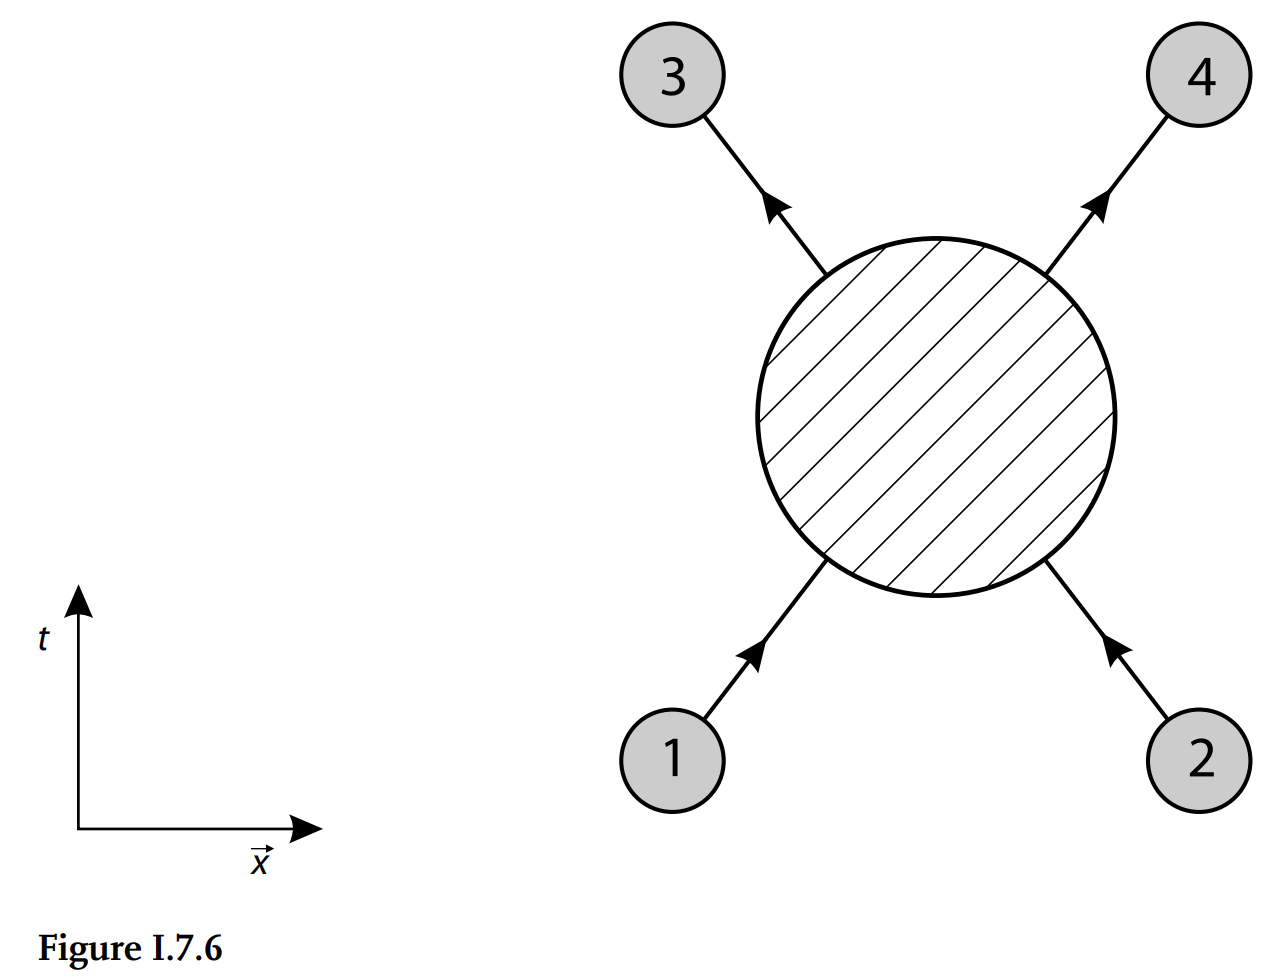
\includegraphics[scale=0.3]{mesons}
	\caption{From Zee}
\end{figure}\\

It suffices to find in $\Z$ a term containing $J(x_1)J(x_2)J(x_3)J(x_4)$. But we notice that this is just $G^{(4)}(x_1,x_2,x_3,x_4)$.\\

Let's start from the Wick way first. Recall that $G^{(4)}$ is given by
\begin{align}
G^{(4)}(x_1,x_2,x_3,x_4) = \f{1}{\Z(0,0)}\int \mathfrak{D}[\phi]e^{i\int d^4x\, \f{1}{2}[(\p \phi)^2 - m^2\phi^2]- \f{\lambda}{4!}\phi^4}\phi(x_1)\phi(x_2)\phi(x_3)\phi(x_4).
\end{align}
Expanding in $\lambda$ gives
\begin{align}
G^{(4)}(x_1,x_2,x_3,x_4) = \f{1}{\Z(0,0)}&\int \mathfrak{D}[\phi]e^{i\int d^4x\, \f{1}{2}[(\p \phi)^2 - m^2\phi^2]}\nonumber\\
&\times  \phi(x_1)\phi(x_2)\phi(x_3)\phi(x_4) \sum^\infty_{s=0}\f{\lp - \f{i\lambda}{4!}\int d^4w\,\phi^4(w)\rp^s}{s!}.
\end{align}
To first order, i.e., $s=1$, we have
\begin{align}
G^{(4)}(x_1,x_2,x_3,x_4) = \f{1}{\Z(0,0)}&\lp \f{-i\lambda}{4!} \rp\int d^4w\int \mathfrak{D}[\phi]e^{i\int d^4x\,\f{1}{2}[(\p \phi)^2 - m^2\phi^2]}\nonumber\\ &\times\phi(x_1)\phi(x_2)\phi(x_3)\phi(x_4)\phi^4(w).
\end{align}
By staring at this integral for a bit we recognize that it is a more complicated case of the high-moment Gaussian integral we have encountered before in Eq \eqref{high-moment}, where the sum in simply replaced by an integral, and the overall integral is multiplied by a factor of $i$. Once again, $\phi(x_1)$ has four choices of $\phi(w)$ to contract with, and so on, so that in the end the factor of $4!$ is canceled. Once the Feynman's trick to differentiate under the integral sign is done correctly, we will get
\begin{align}\label{four-sources}
\boxed{G^{(4)}(x_1,x_2,x_3,x_4) = \f{-i\lambda}{\Z(0,0)}\int d^4w\, \D(x_1 - w)\D(x_2 - w)\D(x_3 - w)\D(x_4 - w)}
\end{align}
which not surprisingly completely shares the structure of Eq \eqref{high-moment}. Now, compare this to what we found when we tried to show $G^{(2)} = i\D$, we see that we wouldn't be quite right to just set $G = $ products of $\D$. What we see here is that $G$ is a summation over all possible products of $\D_{iw}$ over all $w$. This is the accurate relationship between the Green's functions and the propagators. It follows from this that $G^{(2)}_{ab} = i\D_{ab}$.  \\

What about the Schwinger way where we first expand in $J$? Well, we start out with
\begin{align}
\Z(J) = \Z(0,0)e^{ -i\lambda/4! \int d^4w\, [\delta/i \delta  J(w)]^4 } e^{ (-i/2)\iint d^4x d^4y\, J(x)\D(x-y)J(y) }
\end{align}
and replace the first exponential with only first order terms in $J$. Once this is done, we get
\begin{align}
\Z(J) = \Z(0,0)\lb -\lp\f{i\lambda}{4!}\rp \int d^4w \lp \f{\delta}{\delta J(w)} \rp^4 \rb e^{ (-i/2)\iint d^4x d^4y\, J(x)\D(x-y)J(y) }.
\end{align}
Next, we expand the exponential and find the term with the fourth order of $\D$ (since we're looking for a term describing four propagations)
\begin{align}
e^{ (-i/2)\iint d^4x d^4y\, J(x)\D(x-y)J(y) } = \sum^\infty_{s=0}\f{[(-i/2)\iint d^4x d^4y\, J(x)\D(x-y)J(y)]^s}{s!}.
\end{align}
The fourth order term is 
\begin{align}
\f{1}{4!}\lp \f{-i}{2} \rp^4\lb \iint d^4x d^4y\, J(x)\D(x-y)J(y)  \rb^4.
\end{align}
Thus the term in first order $\lambda$ and fourth order $\D$ is
\begin{align}
\lb -\lp\f{i\lambda}{4!}\rp \int d^4w \lp \f{\delta}{\delta J(w)} \rp^4 \rb\lp\f{1}{4!}\rp\lp \f{-i}{2} \rp^4\lb \iint d^4x d^4y\, J(x)\D(x-y)J(y)  \rb^4.
\end{align}
After some cleaning up the algebra and renaming we get
\begin{align}\label{multi-J}
\boxed{\sim i\lambda \int_w \lp \f{\delta}{\delta J(w)} \rp^4 \bigintss^{(8)}  \D_{ae}\D_{bf}\D_{cg}\D_{dh}J_aJ_bJ_cJ_dJ_eJ_fJ_gJ_h}
\end{align}
where the very big integral denotes 8 integrals; $\D_{ij} \equiv \D(x_i - x_j)$; $J(x_a) = J_a$; $\int_a = \int d^4x_a$. \\

We notice that the four $[\delta/\delta J(w)]$'s will hit the $J$'s of course. The $\delta/\delta J(w)$ acts like a delta function:
\begin{align}
\f{\delta}{\delta J(w)}J_a = \delta(a-w).
\end{align}
So, for example.
\begin{align}
\f{\delta}{\delta J(w)}\int \D_{ae}J_e = \int \D_{ae}\delta (e-w)J_e = \D_{aw}.
\end{align}
We can write all this out, but in the end not all terms will be of interest of us. In particular, there will be three terms, two of which are disconnected (so the $\D_{ij}$'s don't share any common $x_i$). The only connected term is:
\begin{align}
\sim -i\lambda \int_w  \iiiint \D_{aw}\D_{bw}\D_{cw}\D_{dw}J_aJ_bJ_cJ_d
\end{align}
where we have reduced the number of integrals because of the delta function. \\

Okay. Why did we do all of this? The \textbf{goal} here is to see two particles (mesons) created by some localized source, scatter off each other, and disappear into localized sinks. So, if we set the source and sinks to be delta functions:
\begin{align}
J_i = \delta(x - x_i), \hspace{1cm} x = 1,2,3,4
\end{align}
then we have
\begin{align}
&-i\lambda \int_w  \iiiint \D_{aw}\D_{bw}\D_{cw}\D_{dw}J_aJ_bJ_cJ_d \\
=\,\,&i\lambda \int_w  \iiiint \D_{aw}\D_{bw}\D_{cw}\D_{dw}\delta(1)\delta(2)\delta(3)\delta(4) \\ 
=\,&\boxed{-i\lambda \int_w \D_{1w}\D_{2w}\D_{3w}\D_{4w}}
\end{align}
This is exactly what we found in Eq \eqref{four-sources}, up to some constants we haven't accounted for of course. \\

What does it all mean? The result is this: 2 particles from $x_1$ and $x_2$ propagate to the spacetime point $w$ (\textit{every possible $w$}), with amplitude $\D(x_1 - w)\D(x_2 - w)$, scatter with amplitude $-i\lambda$, then propagate from $w$ to $x_3$ and $x_4$ with amplitude $\D(x_3 - w)\D(x_4 - w)$. The integration over all spacetime $\int_w \equiv \int d^4w$ just means that the propagation to $w$ could have been anywhere. This comes back to the child problem!
\begin{figure}[!htb]
	\centering
	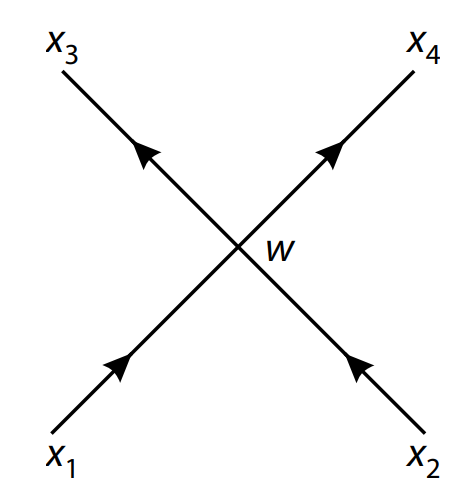
\includegraphics[scale=0.3]{propagates}
	\caption{From Zee}
\end{figure}















\subsubsection{Feynman diagrams: The rules}

So what are the rules for Feynman diagrams? Do we have to do all this integration and expansion every time to calculate the Green's function/correlation function? I think it's clear at this point a lot we have done so far has been by analogy: we begin to form associations between objects such as $q \to \phi$, sum $\to$ integral, and so on. What are the underlying rules here? What is the relationship between Feynman diagrams in position (spacetime) space and momentum space? \\

Sometimes it is easier for us to go pass to momentum space. Hypothetically, a particle with momentum $k_1$ and a particle with momentum $k_2$ collide and scatter, emerging with momentum $k_3$ and $k_4$. Each spacetime propagator has the form
\begin{align}
\D(x_a - w) = \F[\D(k_a)](x_a) = \int \f{d^4k_a}{(2\pi)^4} \f{e^{\pm ik_a(x_a - w)}}{k_a^2 - m^2 + i\epsilon}
\end{align}
where $\F$ denotes the Fourier transform of course and the sign assignment to $k_a$ can be made arbitrary because the ``volume'' element always corrects for that. Thus the overall $G^{(4)}$ (or the correlation function) up to leading constants has the form:
\begin{align}
-i\lambda \int_w \D_{1w}\D_{2w}\D_{3w}\D_{4w} &\sim \int d^4w \, \exp\lp -i(k_1 + k_2 - k_3 - k_4) \rp \\
&= (2\pi)^4\delta^{(4)}(k_1 + k_2 - k_3 - k_4).
\end{align}
So, the fact that the interaction can occur anywhere in spacetime translate to conservation of momentum:
\begin{align}
k_1 + k_2 = k_3 + k_4.
\end{align}
\begin{figure}[!htb]
	\centering
	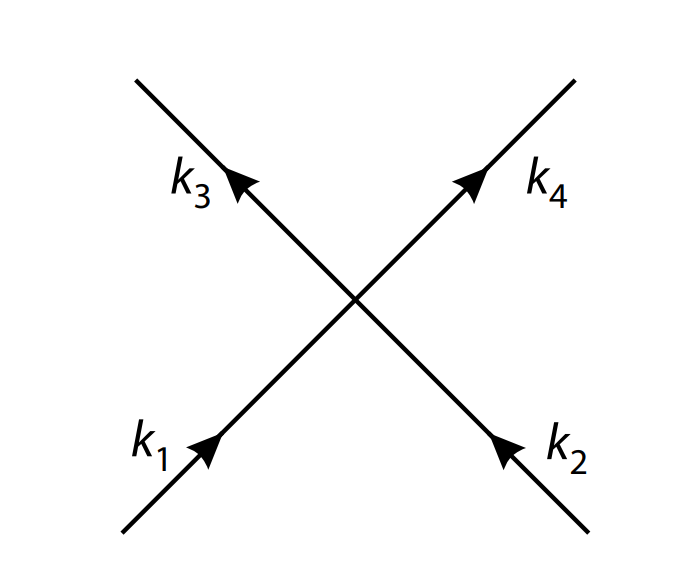
\includegraphics[scale=0.3]{momentum-propagator}
	\caption{From Zee}
\end{figure}
So we have Feynman diagrams for both position and momentum space. Spacetime Feynman diagrams are just literal pictures of what happened. For momentum space Feynman diagrams, here are the rules to calculate the Green's function for a given process:
\begin{enumerate}
	\item Draw a Feynman diagram of the process.
	\item Label each line with a momentum $k$ and associate with it the propagator
	\begin{align}
	\D(k) = \f{i}{k^2 - m^2 + i\epsilon}.
	\end{align}
	Note that we are in momentum space, so the propagator is just this. 
	\item Associate with each interaction vertex (where four lines meet) the coupling 
	\begin{align}
	-i\lambda \hspace{1cm} \text{and} \hspace{1cm}  2\pi^4\delta^{(4)}\lp\sum_i k_i -\sum_j k_j\rp,
	\end{align}
	forcing the sum of momenta $\sum_i k_i$ coming into the vertex to be equal to the sum of momenta $\sum_j k_j$ going out of the vertex. (Note that the act of associating $\lambda$ to an interaction vertex is exactly what we did in the baby problem.)
	\item Momenta associated with internal lines are to be integrated over with the measure $d^4k / (2\pi)^4$, where $k$ denotes the internal/intermediate momentum. Incidentally, this corresponds to the summation over intermediate states in ordinary perturbation theory. 
	\item We have to be careful about symmetry factors. They are the analogs of those numerical factors in the baby problem. As a result, some diagrams are to be multiplied by a symmetry factor such as $1/2$. These come from various combinatorial factors counting the different ways in which the $\delta/\delta J$'s can hit the $J$'s in the multiple integral like \eqref{multi-J}.
	\item We also do not associate a propagator with external lines. 
	\item A delta function for overall momentum conservation is understood. 
\end{enumerate}\qed\\


For example, we can try the diagram we just saw:

\begin{figure}[!htb]
	\centering
	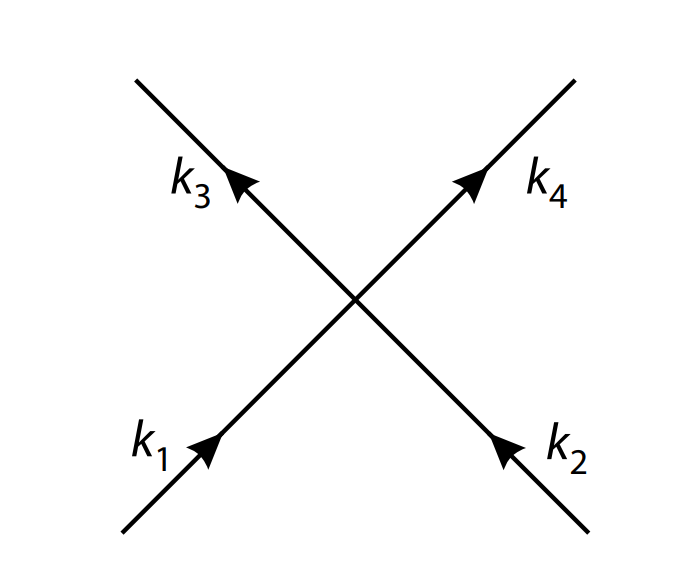
\includegraphics[scale=0.3]{momentum-propagator}
	\caption{From Zee}
\end{figure}

Applying the rules, we obtain
\begin{align}
(-i\lambda)(2\pi)^4\delta^{(4)}(k_1 + k_2 - k_3 - k_4)\prod^4_{a=1}\lp \f{i}{k_a^2 - m^2 + i\epsilon} \rp.
\end{align}

The big multiplicative factor is common to all diagrams in which two mesons scatter into two mesons. So we will just assume it is there and ignore that it is there. This procedure is called ``amputating external legs.'' We also have that in real experiments $k_a^2 = m^2$ since the momentum and mass are equivalent when $c=1$. There are some technical things which we will deal with later. We also see that because momentum must be conserved, we shouldn't worry too much about the delta function either. So same with the other factor, we will just assume it's there and don't write it. \\

With these rules, the amplitude we obtain is denoted by $\mathcal{M}$. For the diagram above, 
\begin{align}
\mathcal{M} = -i\lambda.
\end{align}






















\subsubsection{Birth of particles}



In this section we will describe how two colliding mesons can produce four mesons. 
\begin{figure}[!htb]
	\centering
	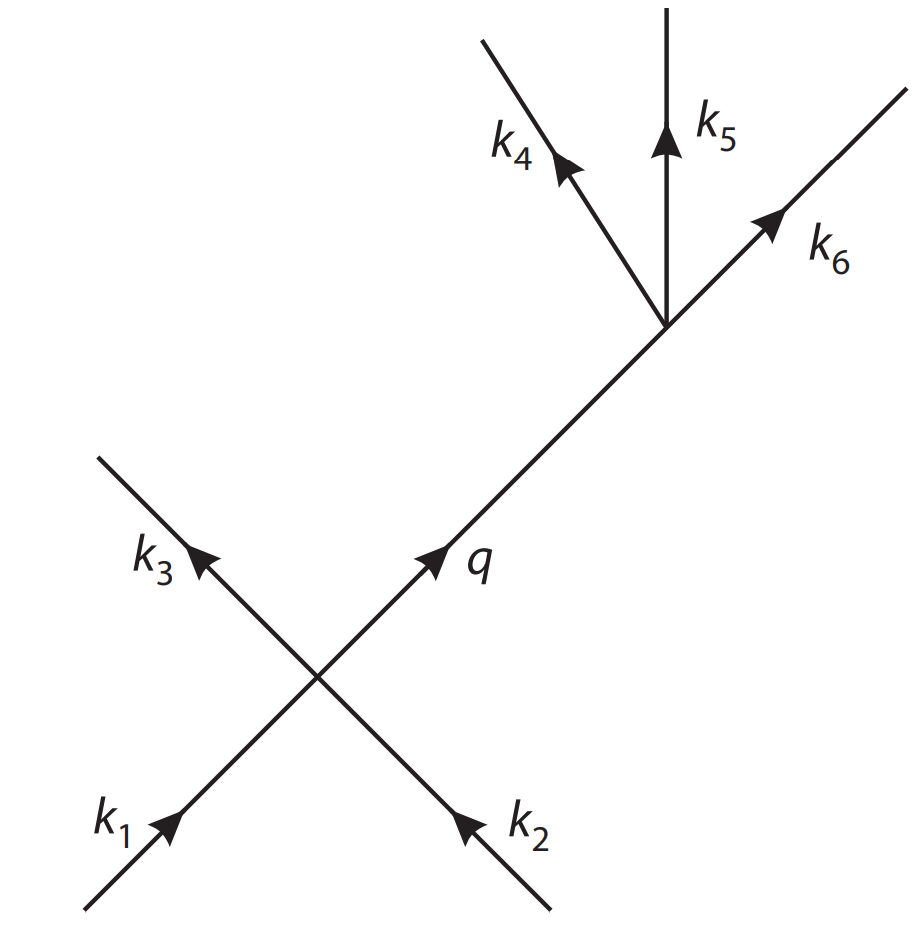
\includegraphics[scale=0.3]{birth}
	\caption{From Zee}
\end{figure}


The process above can occur in $\lambda^2$ perturbation theory. Let us use Feynman's rules to calculate the Green's function/correlation function $G$ for this process. \\

First, the Feynman diagram is already given to us. Good. We would like to calculate the Green's function associated with this diagram.\\

Second, there are $6$ external vertices, so we \textbf{drop} the factor 
\begin{align}
\prod^6_{a=1}\f{i}{k_a^2 - m^2 + i\epsilon},
\end{align}
keeping only the propagator associated with the one internal line, which is
\begin{align}
\f{i}{q^2 - m^2 + i\epsilon}
\end{align} \\

Third, we associate with each interaction vertex a $-i\lambda$. Since there are two of these, we will have a factor of $(-i\lambda)^2$. Next, at the lower vertex we have a factor of $(2\pi)^4\delta^{(4)}\lp k_1 + k_2 - p - k_3 \rp$. At the higher vertex we have a factor of $(2\pi)^4\delta^{(4)}\lp q - k_4 - k_5 - k_6 \rp$. This leaves us with the integrand:
\begin{align}
(-i\lambda)^2 (2\pi)^4\delta^{(4)}\lp k_1 + k_2 - p - k_3 \rp (2\pi)^4\delta^{(4)}\lp q - k_4 - k_5 - k_6 \rp.
\end{align}

Fourth, we integrate the whole term over with the measure $d^p/(2\pi)^4$, since $p$ is the internal momentum here
\begin{align}
(-i\lambda)^2\int \f{d^4 q}{(2\pi)^4} \f{i}{q^2 - m^2 + i\epsilon} (2\pi)^4\delta^{(4)}\lp k_1 + k_2 - p - k_3 \rp \nonumber\\
\hspace{2cm}\times(2\pi)^4\delta^{(4)}\lp q - k_4 - k_5 - k_6 \rp.
\end{align}
Integrals involving delta functions are \textit{very} easy to do. We simply take $q = k_4 + k_5 + k_6$. We should get
\begin{align}
(-i\lambda)^2 \f{i}{(k_4 + k_5 + k_6)^2 - m^2 + i\epsilon} (2\pi)^4\delta^{(4)}(k_1 + k_2 - k_3 - k_4 - k_5 - k_6). 
\end{align}

Finally, the delta function for overall momentum conservation is understood, so 
\begin{align}\label{6-momentum}
\mathcal{M} = (-i\lambda)^2 \f{i}{(k_4 + k_5 + k_6)^2 - m^2 + i\epsilon}
\end{align}
is our answer.\qed











\subsubsection{Cost of not being real}

So what is this relativistic 4-momentum $q = k_4 + k_5 + k_6$? It is the momentum associated with the virtual particle! We notice that $(k_4 + k_5 + k_6)^2$ is not necessarily $m^2$, as it would have to be if the particle were real. The farther the momentum of the virtual particle is from the mass shell $m^2$ the smaller the amplitude, from Eq \eqref{6-momentum}. This makes good sense as the ``cost of not being real.''\\

We can in fact compute Eq \eqref{6-momentum} up to some delta functions and multiplicative factors, just to make sure we understand how the path integral works. But we won't worry about that for now since we have been quite detailed in the previous section. It would be a very good but rather time-consuming exercise.




\subsubsection{Loops and a first look at divergence}

Now, recall from the baby problem that we have both loop and tree diagrams. Loop diagrams are associated with at least a $\lambda$ but no $J$. It is quite similar here in the actual problem. Consider the following Feynman diagram:
\begin{figure}[!htb]
	\centering
	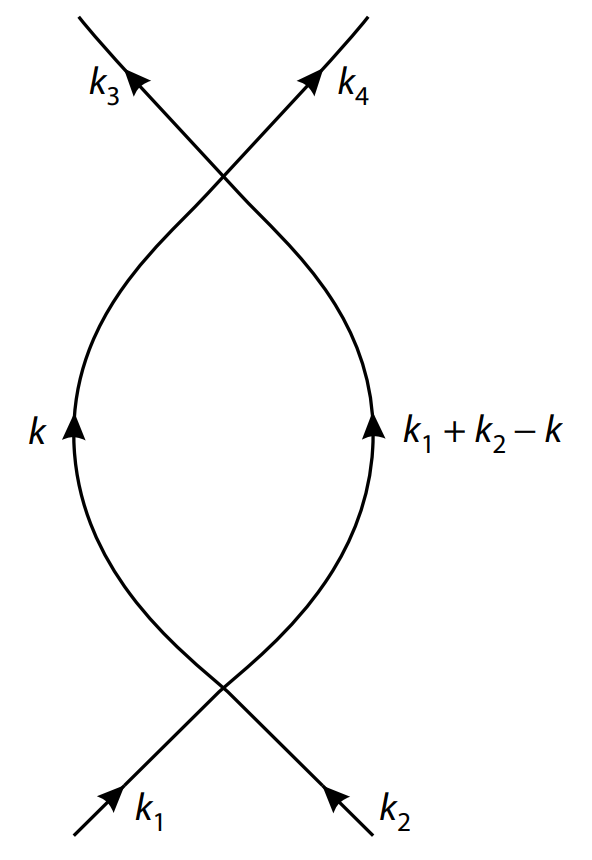
\includegraphics[scale=0.3]{loop-feynman}
	\caption{From Zee}
\end{figure}

We see that there are 2 internal vertices where 4 lines cross. So we get a factor of $(-i\lambda)^2$. We also have 2 factors of internal momentum, after taking into account two delta functions for $k$:
\begin{align}
\f{i}{k^2 - m^2 + i\epsilon} \text{ and } \f{i}{(k_1 + k_2 - k)^2 - m^2 + i\epsilon}.
\end{align}
There is a symmetry factor of $1/2$, since there are two ways this process can occur. We also have some extra factors of $(2\pi)^4$ but we will eventually drop then in the end with one leftover delta function. So the Green's function up to some factor is
\begin{align}
\f{1}{2}(-i\lambda)^2\int \f{d^4k}{(2\pi)^4}\f{i}{k^2 - m^2 + i\epsilon}\f{i}{(k_1 + k_2 - k)^2 - m^2 + i\epsilon}.
\end{align}


This integral blows up only if one of the integrals blow up, i.e., the virtual particle is closest to being real. This is also a cost of not being real. \\

But notice that for large $k$, the integrand goes as $1/k^4$, which means the integral diverges. This is no good! We will come back to this later.\\

Success comes with practice. The more we calculate Feynman diagrams the better we get at doing them by inspection. Here is another example. I won't go into detail what the steps involved are, but we can convince ourselves that the Green's function associated with the following Feynman diagram
\begin{figure}[!htb]
	\centering
	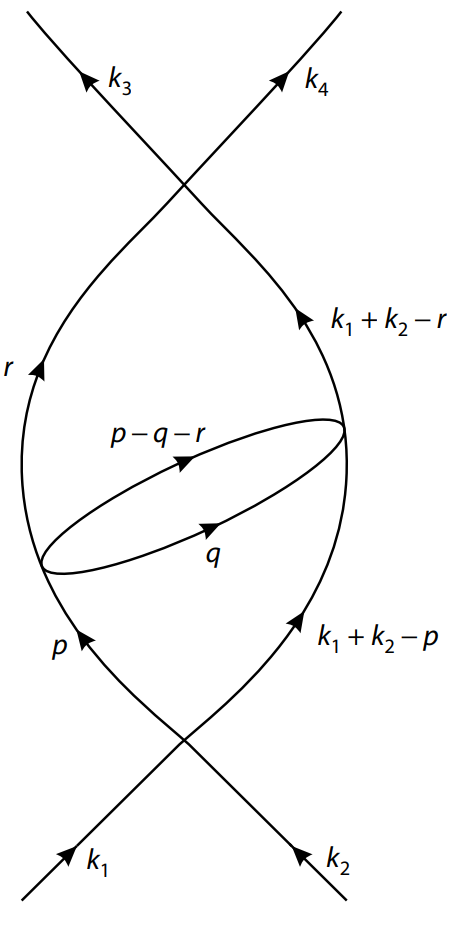
\includegraphics[scale=0.3]{loop-2}
	\caption{From Zee}
\end{figure}

up to symmetry factors and other factors that we don't write down is 
\begin{align}
&(-i\lambda)^4 \int \f{d^4p}{(2\pi)^4}\f{d^4q}{(2\pi)^4}\f{d^4r}{(2\pi)^4} \f{i}{p^2-m^2 +i\epsilon}\f{i}{(k_1+k_2-p)^2-m^2 +i\epsilon}\nonumber\\ &\,\times\f{i}{q^2-m^2 +i\epsilon}\f{i}{(p-q-r)^2-m^2 +i\epsilon}\f{i}{r^2-m^2+i\epsilon}\f{i}{(k_1+k_2-r)^2-m^2 +i\epsilon}
\end{align}





\subsubsection{Vacuum fluctuations}


Let us revisit the self-interaction term we neglected in the full expression 
\begin{align}
i\lambda \int_w \lp \f{\delta}{\delta J(w)} \rp^4 \bigintss^{(8)}  \D_{ae}\D_{bf}\D_{cg}\D_{dh}J_aJ_bJ_cJ_dJ_eJ_fJ_gJ_h
\end{align}
for the Green's function in first order of $\lambda$. Recall that we only kept terms without $\D_{ww}\D_{ww}$ when the $\delta/\delta J(w)$ could have hit $J_c, J_d, J_h, J_g$, resulting in
\begin{align}
-i\lambda \iiiint \D_{ae}\D_{bf} J_a J_b J_eJ_f \lp \int_w \D_{ww}\D_{ww} \rp.
\end{align}
How exactly does this happen? Well,
\begin{align}
\f{\delta}{\delta J(w)}J_j = \delta(x_j - w),
\end{align}
setting $w \to c,d,g,h$, creating $\D_{ww}\D_{ww}$. In this case, the coefficient of $J(x_1)J(x_2)J(x_3)J(x_4)$ us then
\begin{align}
\D_{13}\D_{24} (-i\lambda)\int_w \D_{ww}\D_{ww}
\end{align}
plus other terms by permuting. Because the subscripts of $\D_{13}$ and $\D_{24}$ don't overlap (obviously), we get disconnected diagrams. Also, because we have $\D_{ww}\D_{ww}$, we also get a self-interaction. The associated spacetime Feynman diagram is then
\begin{figure}[!htb]
	\centering
	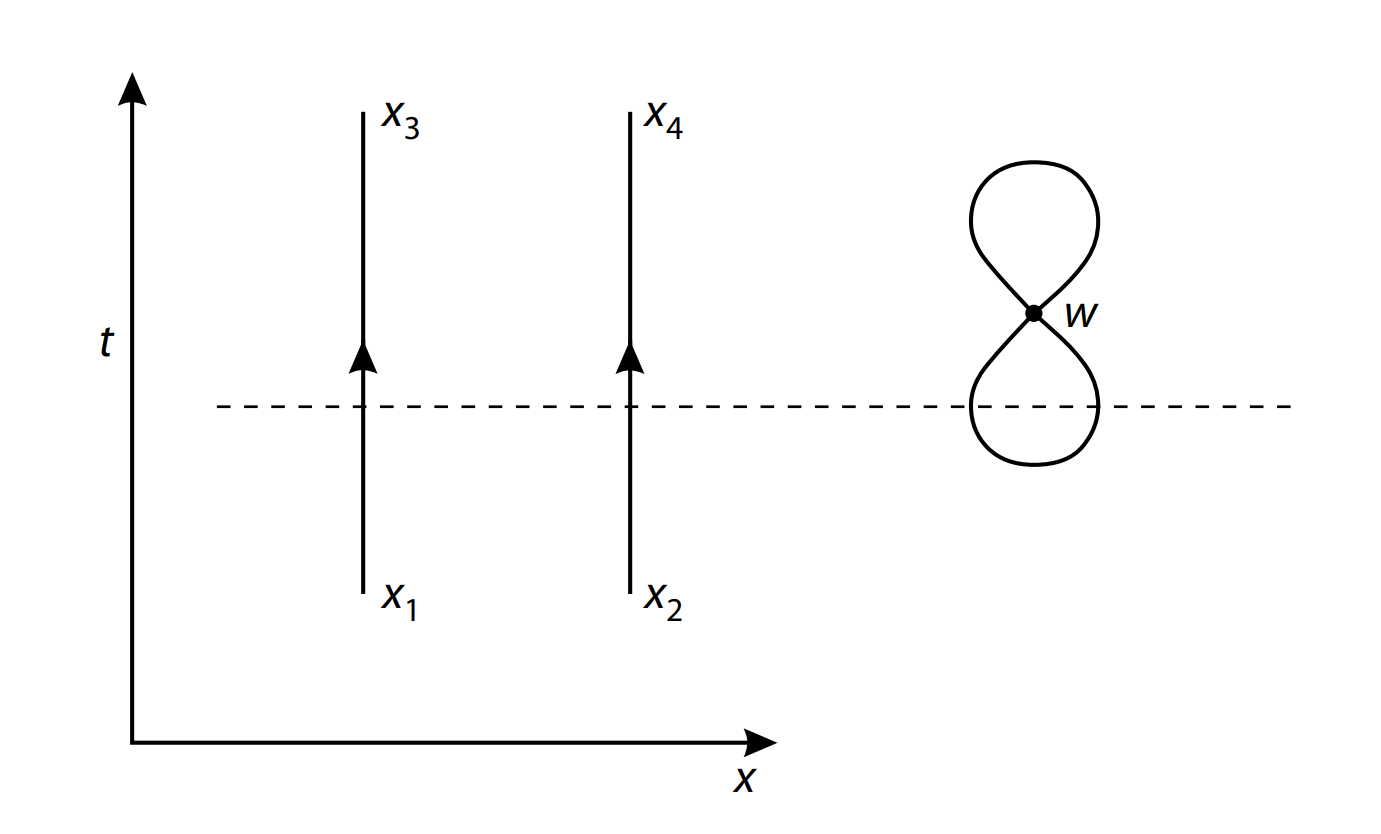
\includegraphics[scale=0.3]{self-int}
	\caption{From Zee}
\end{figure}


Let's describe the underlying physical process: The source at $x_1$ produces a particle that propagates freely without any interaction to $x_3$, where it disappears. A similar thing happen to a particle starting at $x_2$ and ending at $x_4$. These two particles don't interact (disconnected). Now, somewhere off at the point $w$, which could really be \textit{anywhere}, there was an interaction with amplitude $-i\lambda$. This is known as a \textbf{vacuum fluctuation}.\\


Now, when quantum mechanics and special relativity comes together, particles inevitably pop in and out of the vacuum. They could also even interact before vanishing again into the vacuum. From the figure, we see that in the far past, the universe has no particles. Then there are two, then four, then two, then none. We will deal with these fluctuations in better details later. \\

Note that we have seen vacuum fluctuations in the Feynman diagrams in our baby and child problems. We just didn't talk about them!











\newpage









\subsection{Canonical Quantization}




\subsubsection{Heisenberg \& Dirac}


Consider a classical Lagrangian for a single particle
\begin{align}
\boxed{\lag = \f{1}{2}\dot{q}^2 - V(q)}
\end{align}
setting the mass to 1. The canonical momentum is defined by
\begin{align}
p \equiv \f{\delta \lag }{\delta \dot{q}}.
\end{align}
The Hamiltonian is then given by
\begin{align}\label{hamilton}
\ham = p\dot{q} - \lag = \f{p^2}{2} + V(q).
\end{align}

In the Heisenberg formulation, position $q(t)$ and momentum $p(t)$ are promoted to operators which follow the commutation relations:
\begin{align}
\boxed{[p,q] = -i}
\end{align}
where we have set $\hbar = c = 1$. Operators evolve in time according to Heisenberg's equation of motion
\begin{align}
\boxed{\f{dp}{dt} = i[\ham , p] = -\p_q V(q)} \text{ and } \boxed{\f{dq}{dt} = i[\ham , q] = p}
\end{align}
where we have assumed these operators are not explicitly time-dependent. \\

Any operator $O$ constructed out of $p,q$ evolves according to 
\begin{align}
O(t) = e^{i\ham t} O(0) e^{-i\ham t}.
\end{align} 
In particular, consider the following operator:
\begin{align}
a \equiv \f{1}{\sqrt{2w}}\lp wq + ip \rp
\end{align}
defined with some parameter $w$. From the commutation relations between $q$ and $p$, we have that
\begin{align}
\boxed{[a,a^\dagger] = 1}
\end{align}


The evolution of this operator is given by
\begin{align}
\boxed{\f{da}{dt} = i\lb\ham, \f{1}{\sqrt{2w}}(wq + ip)\rb = -i\f{w}{2}\lp ip + \f{1}{w}V'(q) \rp}
\end{align}

The $a$ operator is called the \textit{lowering operator}, defined such that
\begin{align}
\boxed{a\ket{0} = 0}
\end{align}

In the special case of the harmonic oscillator, $V(q) = w^2 q^2/2$, we have that 
\begin{align}
\f{da}{dt} &= -iw a\\
\lag &= \f{1}{2}\dot{q}^2 - \f{1}{2}w^2 q^2\\
\ham &= \f{1}{2}(p^2 + w^2 q^2) = w\lp a^\dagger a + \f{1}{2} \rp\\
[p, q] &= -i.
\end{align}



In general, with multi-particle systems,
\begin{align}
\lag &= \sum_a^N \f{1}{2}\dot{q}_a^2 - V(q_1, q_2, \dots, q_N)\\
p_2 &= \f{\delta \lag}{\delta \dot{q}_a}\\
[p_a(t), q_b(t)] &= -i\delta_{ab}.
\end{align}
where $p_a, q_b$ can be written in terms of the lowering and raising operators. \\


We can also generalize this Lagrangian even further in field theory in $D$-dimensional space:
\begin{align}
\boxed{L = \int d^Dx\, \underbrace{\lc \f{1}{2}[\dot{\phi}^2 - (\grad{\phi})^2 - m^2 \phi^2] - u(\phi) \rc}_{\lag}}
\end{align}
where $u(\phi)$ denotes anharmonic terms. \\

In this case, the canonical momentum density conjugate to the field $\phi(\vec{x},t)$ is given by
\begin{align}
\boxed{\pi (\vec{x} ,t) = \f{\delta \lag}{\delta\dot{\phi}(\vec{x},t)} = \p_0 \phi(\vec{x},t) }
\end{align}
And it follows that the commutation relation (at equal times) now reads
\begin{align}
\boxed{\lb \pi(\vec{x},t), \phi(\vec{x}',t) \rb = \lb \p_0 \phi(\vec{x},t), \phi(\vec{x}',t) \rb = -i\delta^{(D)}(\vec{x} - \vec{x}')}
\end{align}


The Hamiltonian can be found from the Lagrangian (density) similar to Eq. $\eqref{hamilton}$ via 
\begin{align}
H = \int d^D x\, \lc \pi(\vec{x},t) \underbrace{\p_0\phi(\vec{x},t)}_{\pi(\vec{x},t)} - \lag \rc = \int d^Dx\, \lc \f{1}{2}\lb\pi^2 + (\grad{\phi})^2 + m^2 \phi^2\rb     + u(\phi) \rc.
\end{align}

When we don't have any anharmonic terms, i.e. $u(\phi) = 0$, we recover the harmonic oscillator. In this case, we have a free scalar field theory, where $\phi$ solves the Klein-Gordon equation:
\begin{align}
(\p^2 + m^2)\phi  = 0
\end{align}
where
\begin{align}
\p^2 = \f{\p^2}{\p t^2} - \grad.
\end{align}
The Klein-Gordon equation is obtained from varying the Lagrangian with respect to the field. \\

We can verify that the solution to this Klein-Gordon equation has the form
\begin{align}
\boxed{\phi(\vec{x},t) = \int \f{d^D k}{\sqrt{(2\pi)^D 2 w_k}} \lb a(\vec{k})e^{-i(w_k t - \vec{k}\cdot\vec{x})} + a^\dagger(\vec{k})e^{i(w_k t - \vec{k}\cdot \vec{x})} \rb}
\end{align}
where 
\begin{align}
w_k = \sqrt{\vec{k}^2 + m^2}.
\end{align}
The factor $\sqrt{2w_k}^{-1}$ is chosen so that we have
\begin{align}
[a(\vec{k}), a^\dagger(\vec{k})] = \delta^{(D)}(\vec{k} - \vec{k}'),
\end{align}
which implies the correct commutation relation for the field and canonical momentum 
\begin{align}
[\p_0 \phi(\vec{x}, t), \phi(\vec{x}', t)]  = -i\delta^{(D)}(\vec{x} - \vec{x}').
\end{align}





In quantum mechanics, the ground state or vacuum is denoted by $\ket{0}$, following the condition
\begin{align}
a(\vec{k})\ket{0} = 0.
\end{align}
Any single particle state with momentum $\vec{k}$ is given by
\begin{align}
a^\dagger(\vec{k})\ket{0} = \ket{k}.
\end{align}
Consider the expectation value $\bra{0}\phi(\vec{x},t)\ket{k}$. We can compute this
\begin{align}
&\bra{0}\phi(\vec{x},t)\ket{k} \nonumber\\
= &\bra{0}\int \f{d^D k'}{\sqrt{(2\pi)^D 2 w_k'}} \lb a(\vec{k'})e^{-i(w_{k'} t - \vec{k}'\cdot\vec{x})} + a^\dagger(\vec{k}')e^{i(w_{k'} t - \vec{k}'\cdot \vec{x})} \rb \lp a^\dagger(k)\ket{0} \rp \nonumber \\ 
= &\bra{0}\int \f{d^D k'}{\sqrt{(2\pi)^D 2 w_k'}} \lb a(\vec{k'}) a^\dagger(\vec{k})e^{-i(w_{k'} t - \vec{k}'\cdot\vec{x})} + \underbrace{a^\dagger(\vec{k}')a^\dagger(\vec{k})e^{i(w_{k'} t - \vec{k}'\cdot \vec{x})} }_{\text{makes an orthogonal vector to $\ket{0} \forall k$}}\rb\ket{0} \nonumber \\ 
= &\bra{0}\int \f{d^D k'}{\sqrt{(2\pi)^D 2 w_k'}} \lb a(\vec{k'}) a^\dagger(\vec{k})e^{-i(w_{k'} t - \vec{k}'\cdot\vec{x})}\rb\ket{0} \nonumber \\ 
= &\int \f{d^D k'}{\sqrt{(2\pi)^D 2 w_k'}} \lb \bra{0} a(\vec{k'}) a^\dagger(\vec{k})\ket{0}e^{-i(w_{k'} t - \vec{k}'\cdot\vec{x})}\rb \nonumber \\ 
= &\int \f{d^D k'}{\sqrt{(2\pi)^D 2 w_k'}} \lb e^{-i(w_{k'} t - \vec{k}'\cdot\vec{x})}\rb \delta^{(D)}(\vec{k} - \vec{k}') \nonumber\\
= & \boxed{\f{1}{\sqrt{(2\pi)^D 2w_k}}e^{-i(w_k t - \vec{k}\cdot\vec{x})}}
\end{align}



To make contact with the path integral formulation let us evaluate $\bra{0}\phi(\vec{x},t)\phi(\vec{0},0)\ket{0}$ for $t > 0$. Before attempting this by writing the entire expression out, we will notice that of the four possible terms $a^\dagger a^\dagger$, $a^\dagger a$, $a a^\dagger$, and $aa$ in the product of the two fields only $a a^\dagger$ survives because of orthogonality relations and the fact that we're staring out with the ground state. With this, we will proceed:
\begin{align}
  &\bra{0}\phi(\vec{x},t)\phi(\vec{0},0)\ket{0} \nonumber\\
= &\iint \f{d^D k}{\sqrt{(2\pi)^D 2w_k}} \f{d^D k'}{\sqrt{(2\pi)^D 2w_{k'}}}
\bra{0}\lc a(\vec{k})e^{-i(w_k t - \vec{k}\cdot\vec{x})} + a^\dagger(\vec{k})e^{i(w_k - \vec{k}\cdot\vec{x})} \rc \lc a(\vec{k}') + a^\dagger(\vec{k}') \rc\ket{0} \nonumber\\
= &\iint \f{d^Dk \,d^Dk'}{(2\pi)^D (2w_k)(2w_{k'})}e^{-i(w_k t - \vec{k}\cdot\vec{x})}\bra{0}a(\vec{k})a^\dagger(\vec{k}')\ket{0}\nonumber\\
= &\iint \f{d^Dk \,d^Dk'}{\sqrt{(2\pi)^D (2w_k)(2w_{k'})}}e^{-i(w_k t - \vec{k}\cdot\vec{x})}\delta^{(D)}(\vec{k} - \vec{k}')\nonumber\\
= &\iint \f{d^Dk \,d^Dk'}{\sqrt{(2\pi)^{2D} (2w_k)(2w_{k'})}}e^{-i(w_k t - \vec{k}\cdot\vec{x})}\delta^{(D)}(\vec{k} - \vec{k}')\nonumber\\
= &\boxed{\int \f{d^D k}{(2\pi)^{D} 2w_k}e^{-i(w_k t - \vec{k}\cdot\vec{x})}}
\end{align}


With this, if we define the time-ordering product 
\begin{align}
\boxed{T[\phi(x)\phi(y)] = \theta(x^0 - y^0) \phi(x)\phi(y) + \theta(y^0 - x^0)\phi(y)\phi(x)}
\end{align}
then we have
\begin{align}
  &\bra{0}T[\phi(\vec{x},t)\phi(\vec{0},0)]\ket{0} \nonumber\\
= &\bra{0}  \theta(t)\phi(x)\phi(0) + \theta(-t)\phi(0)\phi(x)   \ket{0} \nonumber\\
= &\bra{0}  \theta(t)\phi(x)\phi(0)\ket{0} + \bra{0}\theta(-t)\phi(0)\phi(x)  \ket{0} \nonumber\\
= & \boxed{\int \f{d^D k}{(2\pi)^D 2w_k}\lb \theta(t)e^{-i(w_k t - \vec{k}\cdot\vec{x})} + \theta(-t)e^{i(w_k t - \vec{k}\cdot\vec{x})} \rp}
\end{align}

where
\begin{align}
\bra{0} \phi(x)\phi(0) \ket{0} &= \int \f{d^D k}{(2\pi)^D 2w_k}e^{-i(w_k t - \vec{k}\cdot\vec{x})} \\ 
\bra{0} \phi(0)\phi(x) \ket{0} &= \int \f{d^D k}{(2\pi)^D 2w_k}e^{+i(w_k t - \vec{k}\cdot\vec{x})}
\end{align}
which we can check by inspection. Comparing this result to Eq. \eqref{propag}, which we will repeat here:
\begin{align}
\D(x) = \f{-i}{(2\pi)^3}\int \f{d^3k}{ 2 w_k} \lb e^{-i[w_kt - \vec{k}\cdot\vec{x}]}\theta(t) + e^{i[w_kt - \vec{k}\cdot\vec{x} ]}\theta(-t)\rb,
\end{align}
we immediately see that
\begin{align}
\boxed{\bra{0}T[\phi(\vec{x},t)\phi(\vec{0},0)]\ket{0} = i\D(x) = G^{(2)}(x,0)}
\end{align}

This nicely connects quantum mechanics to the path integral formalism. \\

The moral here is that we always create before we annihilate, not the other around. This is a form of causality as formulated in quantum field theory. 






\subsubsection{Scattering amplitude}


In this section we will show how the invariant scattering amplitude $\mathcal{M}$ arises from this formalism. Suppose we would like to evaluate the quantity:
\begin{align}
\boxed{\bra{\vec{k_3}\vec{k_4}}e^{-iH T}\ket{\vec{k_1} \vec{k_2}} = \bra{\vec{k_3}\vec{k_4}}e^{i \int d^4x\, \lag(x) }\ket{\vec{k_1} \vec{k_2}} }
\end{align} 
for the following meson scattering process
\begin{align}
\vec{k_1} + \vec{k_2} \to \vec{k_3}+ \vec{k_4}
\end{align}
in order $\lambda$, with the anharmonic term $u(\phi) = \lambda \phi^4 / 4!$. The ``sandwiched'' term is given by
\begin{align}
&\exp\lc i \int d^4x\,\f{1}{2}\p^\mu \phi \p_\mu \phi - \f{1}{2}m^2\phi^2 - \f{\lambda}{4!}\phi^4(x) \rc
\end{align}
Next, let us expand in $\lambda$ and collect only the term in order $\lambda$. This term is 
\begin{align}
\int d^4x\,\lb i\f{\lambda}{4!}\phi^4(x) \rb \times \exp\lc -i \int d^4x\,\f{1}{2}\lb \p^\mu \phi \p_\mu \phi - m^2\phi^2 \rb \rc.
\end{align}
Next, recall from the \textbf{Perturbative Field Theory} section that we can integrate the integral in the exponent above by parts and show that 
\begin{align}
&\exp\lc -i \int d^4x\,\f{1}{2}\lb \p^\mu \phi \p_\mu \phi - m^2\phi^2 \rb \rc \nonumber\\
= &\exp\lc -i \int d^4x\,\f{-1}{2}\phi\lb \underbrace{ \square + m^2}_{A} \rb\phi \rc \nonumber\\
= &\exp\lc i \int d^4x\,\lp\f{1}{2}\phi A \phi\rp \rc.
\end{align}
Now, because $\phi$ is the solution to the free field (Klein-Gordon) equation, we must have that
\begin{align}
(\square + m^2)\phi = A\phi = 0 \implies \exp\lc -i \int d^4x\,\f{1}{2}\lb \p^\mu \phi \p_\mu \phi - m^2\phi^2 \rb \rc \equiv 1. 
\end{align}
Thus,
\begin{align}
\boxed{\bra{\vec{k_3}\vec{k_4}}e^{-iH T}\ket{\vec{k_1} \vec{k_2}} \approx \lp -i\f{\lambda}{4!} \rp\int d^4x \, \bra{\vec{k_3}\vec{k_4}}\phi^4(x)\ket{\vec{k_1} \vec{k_2}}}
\end{align}
  
  
How do we actually calculate this? There is some similarity between what we have done and what we have here. Before, we have a product of two fields sandwiched between the ground states. Now, we have four, sandwiched between two four-particle states. In order to correct describe the picture, we need to annihilate $\ket{\vec{k_1}}$ and $\ket{\vec{k_2}}$ then create $\ket{\vec{k_3}}$ and $\ket{\vec{k_4}}$. Thus we look for the term $a^\dagger(\vec{k_4}) a^\dagger(\vec{k_3})a(\vec{k_2})a(\vec{k_1})$. The $a(\vec{k_1})$ term could come from any of the four fields $\phi$. The $a(\vec{k_2})$ terms cold come from any of the leftover three fields, and so on. In the end, we have $4!$ of $a^\dagger(\vec{k_4}) a^\dagger(\vec{k_3})a(\vec{k_2})a(\vec{k_1})$ terms. This $4!$ cancels with the term in the denominator. The exponential corresponding to this term is 
\begin{align}
e^{ i \lp (w_4 t - \vec{k}_4 \cdot \vec{x}) + (w_3 t - \vec{k}_3 \cdot \vec{x}) - (w_2 t - \vec{k}_2 \cdot \vec{x}) - (w_1 t - \vec{k}_1 \cdot \vec{x})\rp } \equiv e^{i (k_3 + k_4 - k_1 - k_2)\cdot x}.
\end{align}
So, the matrix element is 
\begin{align}
\lp \prod^4_{\alpha = 1} \f{1}{\sqrt{(2\pi)^D 2 w_\alpha}} \rp \int d^4x\, e^{i (k_3 + k_4 - k_1 - k_2)\cdot x} 
\end{align}
Finally, recall that
\begin{align}
\delta^{(4)}(x - y) = \F[1](x-y) \f{1}{(2\pi)^4}\int d^4p \, e^{i(x-y)p},
\end{align}
so we have the full amplitude: 
\begin{align}
\boxed{\lp -i\lambda \rp \lp \prod^4_{\alpha = 1} \f{1}{\sqrt{(2\pi)^D 2 w_\alpha}} \rp (2\pi)^4 \delta^{(4)}(k_3 + k_4 - k_2 - k_1)}
\end{align}
where we recall that $\mathcal{M}(f \leftarrow i) = -\lambda$.\\

It is conventional to refer to 
\begin{align}
S_{fi} = \bra{f}e^{-iHT}\ket{i}
\end{align}
as the matrix elements of the $S$-matrix. From here, we can define the transition matrix $T$ by 
\begin{align}
S \equiv I + iT \iff S_{fi} = \delta_{fi} + iT_{fi}.
\end{align}
With this, and expressing the change in momentum in general as the sum of final minus the sum of initial momenta, we get
\begin{align}
\boxed{iT_{fi} = (2\pi)^4 \delta^{(4)}\lp \sum_f k - \sum_i k \rp \lp \prod^4_{\alpha = 1} \f{1}{\sqrt{(2\pi)^D 2 w_\alpha}} \rp \mathcal{M}(f \leftarrow i)}
\end{align}




\subsubsection{Energy of the vacuum}


In this section we will find the expectation value $\bra{0}H\ket{0}$ in the free scalar field theory where we have constructed the Hamiltonian from the Lagrangian:
\begin{align}
H = \pi^2 + (\grad{\phi})^2 + m^2 \phi^2.
\end{align}

Recall that we have computed $\phi$:
\begin{align}
\phi(\vec{x},t) = \int \f{d^D k}{\sqrt{(2\pi)^D 2 w_k}} \lb a(\vec{k})e^{-i(w_k t - \vec{k}\cdot\vec{x})} + a^\dagger(\vec{k})e^{i(w_k t - \vec{k}\cdot \vec{x})} \rb.
\end{align}
It follows that
\begin{align}
\pi^2(\vec{x},t) &= [\p_0 \phi(\vec{x},t)]^2 = w_k^2 \phi^2(\vec{x},t)\nonumber\\
(\grad{\phi})^2 &= \vec{k}^2 \phi^2(\vec{x},t) \nonumber.
\end{align}
So we only have to look at $\bra{0}\phi(\vec{x},t)\phi(\vec{x},t)\ket{0}$:
\begin{align}
\bra{0}\phi(\vec{x},t)\phi(\vec{x},t)\ket{0} &=  
\end{align}


We also have that
\begin{align}
&\bra{0}\phi^2(\vec{x},t)\ket{0} \nonumber\\
= &\bra{0}\phi(\vec{x},t)\phi(\vec{x},t)\ket{0} \nonumber\\
= &\bra{0} \lp \int \f{d^Dk}{\sqrt{(2\pi)^D 2w_k}} \lc a(\vec{k})e^{ik\cdot x} + a^\dagger(\vec{k})e^{-ik\cdot x} \rc \rp^2   \ket{0} \nonumber\\
= &\iint \f{d^D k\,d^Dk'}{\sqrt{(2\pi)^{2D}(2w_k)(2w_k')}}\bra{0} \lc a(\vec{k})e^{ik\cdot x} + a^\dagger(\vec{k})e^{-ik\cdot x}  \rc \lc a(\vec{k'})e^{ik'\cdot x} + a^\dagger(\vec{k'})e^{-ik'\cdot x}  \rc \ket{0} \nonumber\\
= &\iint \f{d^D k\,d^Dk'}{\sqrt{(2\pi)^{2D}(2w_k)(2w_k')}}\underbrace{\bra{0} a(\vec{k})a^\dagger(\vec{k}')e^{i(k-k')\cdot x} \ket{0}}_\delta \nonumber\\
= &\iint \f{d^D k\,d^Dk'}{\sqrt{(2\pi)^{2D}(2w_k)(2w_k')}} \delta^{(D)}(k - k')\nonumber\\
= & \int \f{d^D k}{(2\pi)^D 2w_k}.
\end{align}
Putting this together, we find
\begin{align}
\bra{0}H\ket{0} &= \int d^Dx\f{1}{2}\bra{0} \lp \pi^2 + (\grad{\phi})^2 + m^2 \phi^2 \rp\ket{0} \nonumber\\
&= \underbrace{\int d^Dx}_{V}\,  \int \f{d^D k}{(2\pi)^D 2w_k} \f{1}{2} (w_k^2 + \vec{k}^2 + m^2)   \nonumber\\
&= V  \int \f{d^D k}{(2\pi)^D 2w_k} \f{1}{2} (w_k^2 + \underbrace{\vec{k}^2 + m^2}_{w_k^2}) \nonumber\\
&= V  \int \f{d^D k}{(2\pi)^D} \f{1}{2}w_k.
\end{align}
Once $\hbar$ is restored, we get
\begin{align}
\boxed{\bra{0}H\ket{0} = V  \int \f{d^D k}{(2\pi)^D} \f{1}{2}\hbar w_k}
\end{align}
where $V$ the volume of the space. \\


We immediately recognize this as the zero-point energy of the harmonic oscillator integrated over all momentum modes $k$ and over all space. However, we should worry here because this integral over $k$ clearly diverges. However, in reality, we always measure relative to the vacuum, i.e., we are often interested in 
\begin{align}
H - \bra{0}H\ket{0}.
\end{align}
Thus, we won't have to worry about getting infinities here.











\subsubsection{Complex scalar field}

In the previous section, our field is hermitian (or ``real''). In this section, we will look at the formalism for a complex scalar field governed by the Lagrangian density:
\begin{align}
\boxed{\lag = \p \phi^\dagger \p \phi - m^2 \phi^\dagger \phi}
\end{align} 

According to Heisenberg, the canonical momentum is given by
\begin{align}
{\pi(\vec{x},t) = \f{\delta \lag}{\delta \dot{\phi}(\vec{x},t)} = \p_0 \phi^\dagger(\vec{x},t)}
\end{align}
and so 
\begin{align}
{[\pi(\vec{x},t), \phi(\vec{x}',t)] = -i\delta^{(D)}(\vec{x} - \vec{x}')}
\end{align}
just as before. Similarly, we can show that 
\begin{align}
{\pi'(\vec{x},t) = \f{\delta \lag}{\delta \dot{\phi}^\dagger(\vec{x},t)} = \p_0 \phi(\vec{x},t)}
\end{align}

Varying the Lagrangian with respect to the (conjugate of the) field, we get two Klein-Gordon equations:
\begin{align}
{(\square + m^2)\phi = 0; \hspace{0.5cm}(\square + m^2)\phi^\dagger = 0}
\end{align}
 
The Fourier expansion is similar to what we've seen before. However, because $\phi$ is no longer hermitian, we are required to use two independent sets of creation and annihilation operators $(a,a^\dagger)$ and $(b, b^\dagger)$:
\begin{align}
\boxed{\phi(\vec{x},t) = \int \f{d^Dk}{\sqrt{(2\pi)^D 2w_k}}\lb a(\vec{k})e^{-i(w_k t - \vec{k}\cdot\vec{x})} + b^\dagger(\vec{k}) e^{i(w_k t - \vec{k}\cdot\vec{x})}\rb}
\end{align}
The interpretation here is that the particle created by $a^\dagger$ and the particle created by $b^\dagger$ are antiparticles. 


















\newpage









\section{Renormalization \& Gauge Invariance}




\subsection{Cutoffs}







\subsubsection{Field theory blowing up}

Recall the scattering amplitude (or the Green's function) for a $\lambda^2$ loop diagram is given by:
\begin{align}
\mathcal{M} = \f{1}{2}(-i\lambda)^2\int \f{d^4k}{(2\pi)^4}\f{i}{k^2 - m^2 + i\epsilon}\f{i}{(k_1 + k_2 - k)^2 - m^2 + i\epsilon}.
\end{align}
The associated Feynman diagram is
\begin{figure}[!htb]
	\centering
	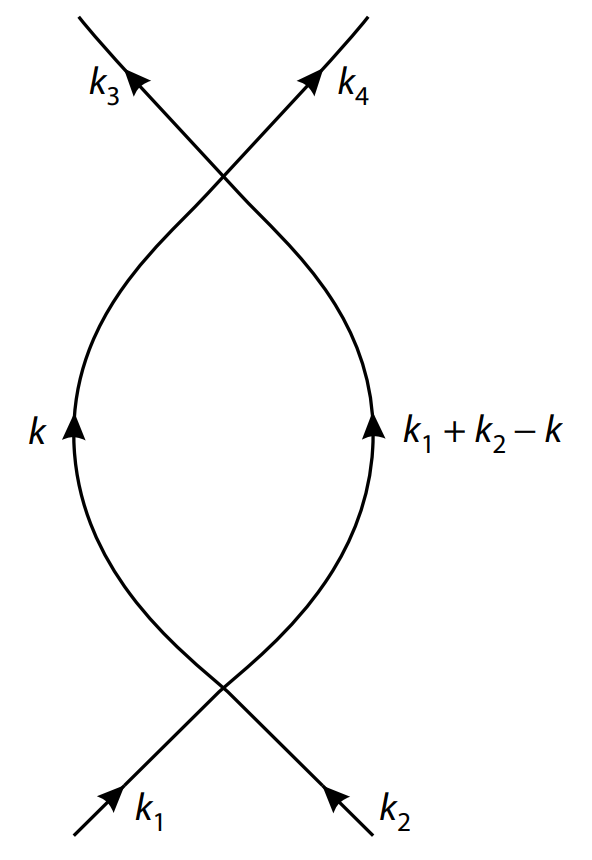
\includegraphics[scale=0.3]{loop-feynman}
	\caption{From Zee}
\end{figure}

We have mentioned in the \textit{Loops and a first look at divergence} that this integral diverges when all momentum modes are considered. How do we deal with this? First, let $K \equiv k_1 + k_2$ denote the total initial momentum. We can rewrite the scattering amplitude as
\begin{align}
\mathcal{M} = \f{1}{2}(-i\lambda)^2\int \f{d^4k}{(2\pi)^4}\f{i}{k^2 - m^2 + i\epsilon}\f{i}{(K - k)^2 - m^2 + i\epsilon}.
\end{align} 

We say that this integral diverges \textit{logarithmically} as $\int d^4k/k^4$ for large $k$. We also call this ``ultraviolet divergence'' since the integral diverges when $k$ is large. \\

To deal with this integral, we have to look at ``regularization'' and ``renormalization.'' \textbf{Regularization} is the process of making divergent integrals converge by integrating up to a cutoff $\Lambda$. Physically, this means that whatever quantum field theory we're working with is an effective low energy theory that is valid up to some energy associated with $\Lambda$.  $\Lambda$ should be thought of as physical, ``parameterizing our threshold of ignorance.'' When we evaluate integrals with a cutoff $\Lambda$, we literally integrate only up to $\Lambda$. If the integral is convergent, we say it is ``regularized.'' So what is
\begin{align}
\mathcal{M} = \f{1}{2}(-i\lambda)^2\int^\Lambda \f{d^4k}{(2\pi)^4}\f{i}{k^2 - m^2 + i\epsilon}\f{i}{(K - k)^2 - m^2 + i\epsilon}?
\end{align}
We might be tempted to evaluate this integral directly by the Cauchy integral formula and the residue theorem. But notice that we are not allowed to do that here because we are integrating over 4-dimensional Minkowskian spacetime. We will learn how to actually do this in the following sections.


\subsubsection{Evaluating Feynman diagrams - Zee's Appendix D}

We would like to evaluate this integral from the previous section:
\begin{align}
\boxed{I = \int \f{d^4k}{(2\pi)^4} \f{1}{(k^2 - c^2+ i\epsilon)^3} = \int \f{d^3k}{(2\pi)^3}\int \f{dk_0}{2\pi} \f{1}{(k_0^2 - (\vec{k}^2 + c^2)+ i\epsilon)^3}} 
\end{align}
where we have used the fact that
\begin{align}
k^2 = k_0^2 - \vec{k}^2
\end{align}
based on the Minkowskian metric. \\

Focusing first on the $k_0$ integral, we observe that if we can somehow turn the denominator into the form:
\begin{align}
k_0^2 - (\vec{k}^2 + c^2) + i\epsilon \to k'^2 + c^2 + i\epsilon
\end{align}
then we no longer have to worry about poles. Whether we can do this depends on whether we can somehow flip the sign of $k_0$ from a plus to a minus to agree with the spatial part of $k$. It turns out this is possible, with a slight change of variables and tricks. Define $k_4$ such that
\begin{align}
k_0 = ik_4.
\end{align}
Then 
\begin{align}
dk_0 = idk_4; \hspace{0.5cm} k_0^2 = -k_4^2.
\end{align}
Next, instead of integrating over the real line and close the contour with the northern semi-contour (or southern semi-contour), we can rotate the contour such that we are integrating over the imaginary line and closing the contour using the east/west contour: 
\begin{figure}[!htb]
	\centering
	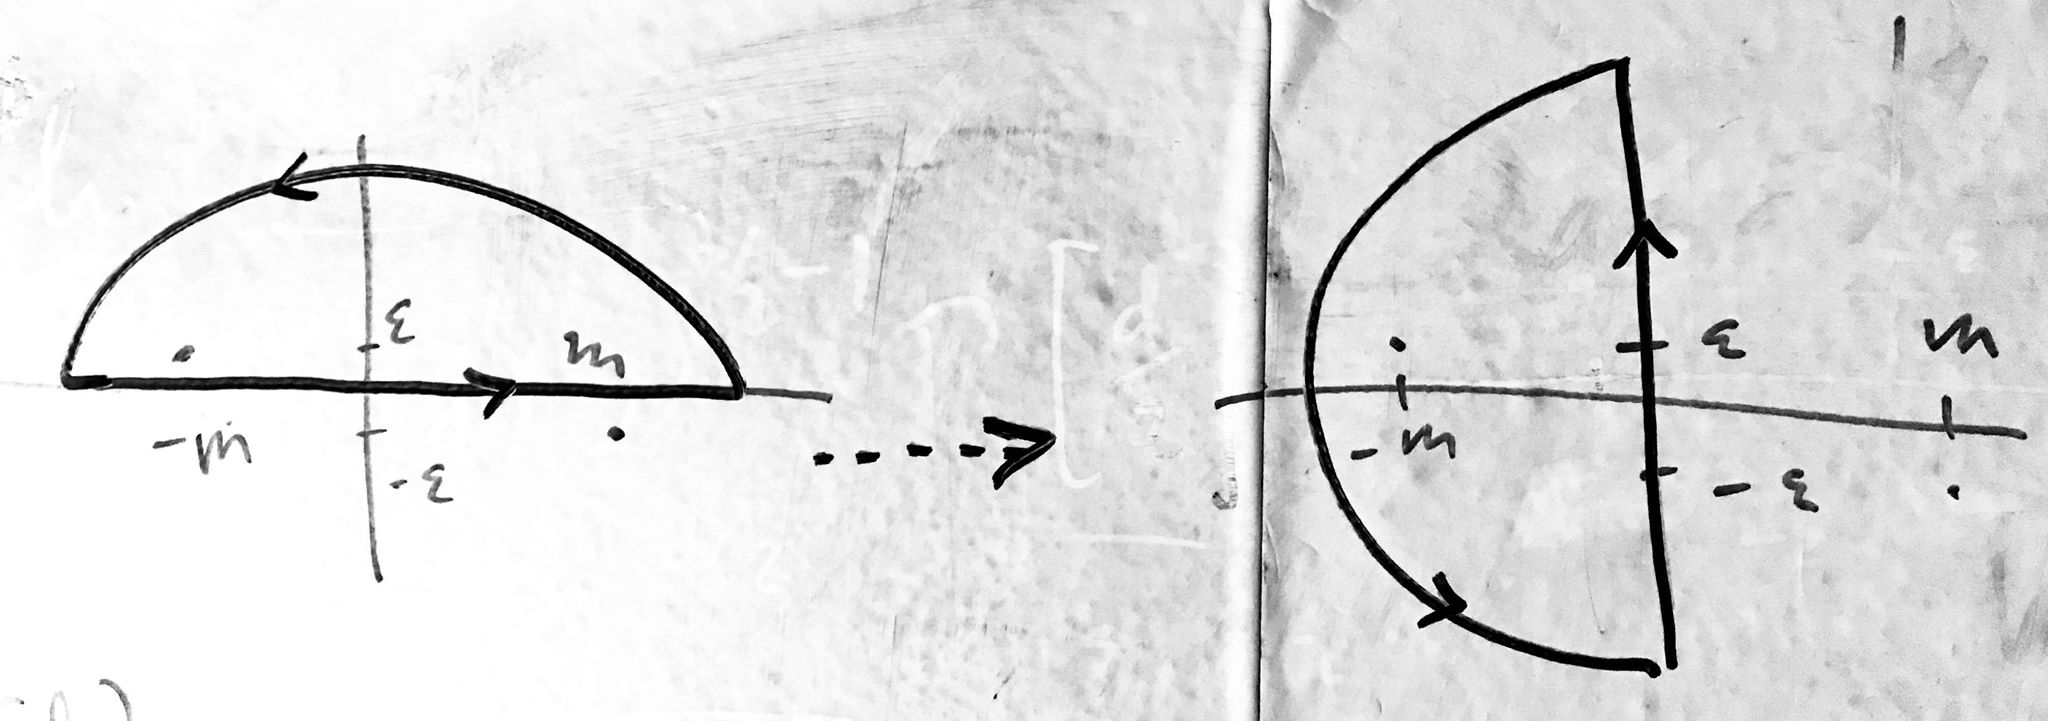
\includegraphics[scale=0.1]{rotate}
\end{figure}

This means
\begin{align}
\int^\infty_{-\infty} dk_0 \f{1}{(k_0^2 - (\vec{k}^2 + c^2)+ i\epsilon)^3} &= \int^{i\infty}_{-i\infty}\f{1}{(k_0^2 - (\vec{k}^2 + c^2)+ i\epsilon)^3} \nonumber\\
&= \int^{-\infty}_{\infty}idk_4\f{1}{(-k_4^2 - (\vec{k}^2 + c^2)+ i\epsilon)^3} \nonumber\\
&= \int^{\infty}_{-\infty}idk_4\f{1}{(\underbrace{k_4^2 + \vec{k}^2} + c^2)^3}; \hspace{0.2cm}\epsilon\to 0 \nonumber\\
&= \int^{\infty}_{-\infty}idk_4\f{1}{(k^2_E + c^2)^3}
\end{align}
where 
\begin{align}
k^2_E = k_4^2 + \vec{k}^2
\end{align}
is the norm square of the Euclidean 4-vector (rather than Minkowskian). With this, we can replace the integration measure
\begin{align}
d^4k \to d^4_Ek
\end{align}
where $d^E k$ is the integration measure in Euclidean 4-dimensional space. So,
\begin{align}
\boxed{I = i(-1)^3\int \f{d^4_E k}{(2\pi)^4} \f{1}{(k^2_E + c^2)^3}}
\end{align}
Good, but how do we evaluate this integral? It turns out that it is more useful for us to look at a more general case where we evaluate
\begin{align}
H = \int d^d_Ek \, F(k^2)
\end{align}
where
\begin{align}
k^2 = k_1^2 + k_2^2 + \dots + k^2_d.
\end{align}
We assume that the integral converges. We will also drop the $E$ subscript for convenience. Suppose we integrate over the $(d-1)$ angular variables to get
\begin{align}
H = C(d)\int^\infty_0 dk\,k^{d-1}F(k^2)
\end{align}
where our $k$ can be thought of as only the radial component. What is $C(d)$? Well, we know that
\begin{align}
J = \int d^dk\, e^{-k^2/2} = \lp\sqrt{2\pi}\rp^d,
\end{align}
from our results in \textit{Gaussian integrals and their moments}. But we know that alternatively,
\begin{align}
J &= \int d^dk\, e^{-k^2/2}\nonumber\\
&= C(d) \int^\infty_0 dk\, k^{d-1}e^{-k^2/2} \hspace{0.5cm}\text{angular-integrated} \nonumber\\
&= C(d) 2^{d/2 - 1} \int^\infty_0 dx\, x^{d/2 - 1}e^{-x} \nonumber\\
&= C(d) 2^{d/2 - 1} \Gamma\lp \f{d}{2} \rp
\end{align}
where we have made the necessary change of variables in order to the get the integral representation of the Gamma function, which shows up quite often in probability theory:
\begin{align}
{\Gamma(z) = \int^\infty_0 x^{z-1}e^{-x}\,dx, \hspace{0.5cm} \Re(z) > 0}
\end{align}
which satisfies the definition of the Gamma function defined for positive integers:
\begin{align}
\Gamma(n) = (n-1)! \iff \Gamma(n+1) = n\Gamma(n),
\end{align}
which we can show by integration by parts. It follows that
\begin{align}
\lp 2\pi \rp^{d/2} = C(d) 2^{d/2 - 1} \Gamma\lp \f{d}{2} \rp,
\end{align}
which means 
\begin{align}
\boxed{C(d) = \f{2\pi^{d/2}}{\Gamma\lp d/2 \rp}}
\end{align}
As a little ``sanity check,'' when $d=2$, when $C(d) = 2\pi$. When $d=3$, $C(d) = 4\pi$, which are familiar angular elements in 2 and 3 dimensions. With this, we have in general,
\begin{align}
\boxed{H = \int d^d_E k \,F(k^2) = C(d)\int^\infty_0 dk\, k^{d-1}F(k^2)= \f{2\pi^{d/2}}{\Gamma\lp d/2 \rp}\int^\infty_0 dk\, k^{d-1}F(k^2)}
\end{align}

So, when $d=4$ (which is the value of $d$ we are interested in), 
\begin{align}
\int d^4_E k \, F(k^2) = (2\pi^2) \int^\infty_0 dk\,k^3 F(k^2).
\end{align}
With this, we can now evaluate the original $I$:
\begin{align}
I &= \int \f{d^4k}{(2\pi)^4} \f{1}{(k^2 - c^2+ i\epsilon)^3}\nonumber\\
&= \dots \nonumber\\ 
&= i(-1)^3\int \f{d^4_E k}{(2\pi)^4} \f{1}{(k^2_E + c^2)^3} \nonumber\\
&= \f{-i}{(2\pi)^4}\int d^4_E k k^3 \f{1}{(k^2 + c^2)^3}  \nonumber\\
&= \f{-i}{(2\pi)^4} (2\pi^2) \underbrace{\int^\infty_0 dk\,k^3   \f{1}{(k^2 + c^2)^3}} \nonumber\\
&= \f{-i}{(2\pi)^4} (2\pi^2) \f{1}{4c^2} \nonumber\\
&= {\f{-i}{32 \pi^2 c^2}},
\end{align}
where the final integral can be evaluated in Mathematica as follows:
\begin{lstlisting}
In[9]:= Integrate[k^3/(k^2 + c^2)^3, {k, 0, Infinity}]

Out[9]= ConditionalExpression[1/(4 c^2), Re[c] != 0]
\end{lstlisting}
$\,$\\

Thus, we have derived the basic formula for doing Feynman integrals:
\begin{align}
\boxed{\int \f{d^4k}{(2\pi)^4} \f{1}{(k^2 - m^2+ i\epsilon)^3} = \f{-i}{32 \pi^2 m^2}}
\end{align}
Okay, what if now we only integrate to a cutoff $\Lambda$ and with a power of $2$ (not $3$) in the denominator, i.e.,
\begin{align}
\int^{k=\Lambda} \f{d^4k}{(2\pi)^4} \f{1}{(k^2 - m^2+ i\epsilon)^2} = ?
\end{align}
Essentially, we can work through the same steps again. Notice that the cutoff is only in $k$ but not in the angular pieces, so we still have that
\begin{align}
\int^{k=\Lambda} \f{d^4k}{(2\pi)^4} \f{1}{(k^2 - m^2+ i\epsilon)^2} &= \f{-i}{(2\pi)^4}(2\pi^2)\int^{k=\Lambda} dk\,k^3\f{1}{(k^2 + m^2)^2}\nonumber\\
&= \f{-i}{8\pi^2}\int^{k=\Lambda} dk\,k^3\f{1}{(k^2 + m^2)^2}
\end{align}
This last integral can be evaluated in Mathematica as follows:
\begin{lstlisting}
In: Integrate[k^3/(k^2 + a^2)^2, {k, 0, L}]

Out: 1/2(-1-Log[a^2])+(a^2+(a^2+L^2)Log[a^2+L^2])/(2(a^2+L^2)) 
\end{lstlisting}

Technical side note: In reality Mathematica gives a bunch of conditional statements, but we can just ignore those since we're only working with positive real numbers here. \\

So, we have
\begin{align}
\int^{\Lambda} \f{d^4k}{(2\pi)^4} \f{1}{(k^2 - m^2+ i\epsilon)^2} &= \f{-i}{16\pi^2}\lc -1 - \log(m^2) + \log(m^2 + \Lambda^2) + \f{m^2 }{m^2 + \Lambda^2} \rc\nonumber\\
&= \f{-i}{16\pi^2}\lc -1  + \log\lp\f{ m^2 + \Lambda^2}{m^2} \rp+ \f{m^2 }{m^2 + \Lambda^2} \rc.
\end{align}

Assuming $\lambda^2 \gg m^2$, we have that
\begin{align}\label{Feynman-int}
\boxed{\int^{\Lambda} \f{d^4k}{(2\pi)^4} \f{1}{(k^2 - m^2+ i\epsilon)^2} \approx \f{i}{16\pi^2} \lb \log\lp \f{\Lambda^2}{m^2} \rp  - 1 + \dots \rb}
\end{align}




As an exercise, let's try to evaluate
\begin{align}
\int^{\Lambda} \f{d^4k}{(2\pi)^4} \f{k^2}{(k^2 - m^2+ i\epsilon)^2}.
\end{align}
Well, we will just a similar thing except for the form of $F(k^2)$. So we have
\begin{align}
\int^{k=\Lambda} \f{d^4k}{(2\pi)^4} \f{k^2}{(k^2 - m^2+ i\epsilon)^2} &= \f{-i}{(2\pi)^4}(2\pi^2)\int^{k=\Lambda} dk\,k^3\f{k^2}{(k^2 + m^2)^2}\nonumber\\
&= \f{-i}{8\pi^2}\int^{k=\Lambda} dk\,\f{k^5}{(k^2 + m^2)^2}.
\end{align}
Once again with the help of Mathematica, we find 
\begin{lstlisting}
In: Integrate[k^5/(k^2 + a^2)^2, {k, 0, L}]

Out: ((2a^2 L^2+L^4+2a^2(a^2+L^2)(Log[a^2]-Log[a^2+L^2]))/(2(a^2+L^2)))
\end{lstlisting}
Thus,
\begin{align}
\int^{k=\Lambda} \f{d^4k}{(2\pi)^4} \f{k^2}{(k^2 - m^2+ i\epsilon)^2} &\approx \f{-i}{16\pi^2}\lc m^2 + \Lambda^2 + 2m^2\log\lp \f{m^2}{m^2 + \Lambda^2} \rp  \rc \nonumber\\
&= \f{-i}{16\pi^2}\lc m^2 + \Lambda^2 - 2m^2\log\lp \f{\Lambda^2}{m^2} \rp + \dots  \rc
\end{align}
where once again we assume $\Lambda^2 \gg m^2$. So we have
\begin{align}
\boxed{\int^{k=\Lambda} \f{d^4k}{(2\pi)^4} \f{k^2}{(k^2 - m^2+ i\epsilon)^2} = \f{-i}{16\pi^2}\lc m^2 + \Lambda^2 - 2m^2\log\lp \f{\Lambda^2}{m^2} \rp + \dots  \rc}
\end{align}




\subsubsection{Denominator Combination Identity - Zee's Appendix D}

Now, for general Feynman integrals/diagrams, we don't often have a single term raised to some power in the denominator such as
\begin{align}
\f{1}{(k^2 - m^2 + i\epsilon)^n}.
\end{align}
For loop diagrams where there are multiple inner loops and possible intermediate momenta, we will have things like
\begin{align}
\f{1}{(k_1^2 - m^2 + i\epsilon)^l} \dots \f{1}{(k_n^2 - m^2 + i\epsilon)^p}
\end{align}
and so on. It is useful we could somehow split this product into a sum of integrals that we can evaluate. Fortunately, we have a useful identity in combining denominators:
\begin{align}
\boxed{\f{1}{x_1\dots x_n} = (n-1)! \int^1_0\dots \int^1_0 d\alpha_1\dots d\alpha_n \, \delta\lp 1 - \sum^n_{j=1} \alpha_j \rp \f{1}{(\alpha_1 x_1 + \dots + \alpha_n x^n)^n}}
\end{align}


For $n=2$, we have
\begin{align}
{\f{1}{xy} = \int^1_0 d\alpha \, \f{1}{[\alpha x +(1-\alpha)y]^2}}
\end{align}
For $n=3$, we have
\begin{align}
\f{1}{xyz} &= 2\int^1_0 \int^1_0 \int^1_0 d\alpha d\beta d\gamma\, \delta(\alpha + \beta + \gamma - 1) \f{1}{[\alpha x + \beta y + \gamma z]^3} \nonumber\\
&= 2\iint_{\text{triangle}} d\alpha d\beta\, \f{1}{[z + \alpha(x-z) + \beta(y -z)]^3}
\end{align}
where the integration region is the triangle in the $\alpha-\beta$ plane bounded by $0 \leq \beta \leq 1 - \alpha$ and $0 \leq \alpha \leq 1$. 
















\subsubsection{Pauli-Villars regularization}

Now we're getting closer to evaluating $\mathcal{M}$ up to cutoff $\Lambda$. To turn the integrand of
\begin{align}
\mathcal{M} = \f{1}{2}(-i\lambda)^2\int \f{d^4k}{(2\pi)^4}\f{i}{k^2 - m^2 + i\epsilon}\f{i}{(K - k)^2 - m^2 + i\epsilon}.
\end{align}
into something we can integrate over, we first apply the following identity from the previous section
\begin{align}
\f{1}{xy} = \int^1_0 d\alpha \f{1}{[\alpha x + (1-\alpha )y]^2}
\end{align}
with 
\begin{align}
y = k^2 - m^2 + i\epsilon \hspace{1cm} x = (K - k)^2 - m^2 + i\epsilon.
\end{align}
Then we have
\begin{align}
\mathcal{M} = \f{1}{2}(-i\lambda)^2 i^2 \int \f{d^4k}{(2\pi)^4}\int^1_0 d\alpha\, \f{1}{D}
\end{align}
where
\begin{align}
D &=  \dots \nonumber \text{some approximations here}\\
& =[\alpha(K-k)^2 + (1-\alpha)k^2 - m^2 + i\epsilon]^2 \nonumber\\
&= [(k - \alpha K)^2 + \alpha(1-\alpha)K^2- m^2   + i\epsilon]^2 \nonumber \hspace{0.5cm}\text{completing the squares}.
\end{align}

Consider the change of variables (called \textit{Feynman variables})
\begin{align}
\kappa =  k - \alpha K \implies d^4k \to d^4\kappa,
\end{align}
then we get
\begin{align}
D = [\kappa^2 + \alpha(1-\alpha)K^2 - m^2 + i\epsilon]^2 = [\kappa^2 - M_0^2 + i\epsilon ]^2
\end{align}
where
\begin{align}
M_0^2 = m^2  - \alpha(1 - \alpha)K^2.
\end{align}
Thus,
\begin{align}
\mathcal{M} &= \f{1}{2}(-i\lambda)^2 i^2 \int \f{d^4\kappa}{(2\pi)^4} \int^1_0 d\alpha\,\f{1}{D} \nonumber\\
&= \f{1}{2}(-i\lambda)^2 i^2 \int \f{d^4\kappa}{(2\pi)^4}  \int^1_0 d\alpha \, \f{1}{[\kappa^2 - M_0^2 + i\epsilon ]^2}\nonumber\\
&= {\f{1}{2}(-i\lambda)^2 i^2  \int^1_0 d\alpha \int \f{d^4\kappa}{(2\pi)^4}  \, \f{1}{[\kappa^2 - M_0^2 + i\epsilon ]^2}}
\end{align}
Imposing a cutoff, we get
\begin{align}
\boxed{\mathcal{M} = \f{1}{2}(-i\lambda)^2 i^2  \int^1_0 d\alpha \int^\Lambda \f{d^4\kappa}{(2\pi)^4}  \, \f{1}{[\kappa^2 - M_0^2 + i\epsilon ]^2}}
\end{align}

Aha! In integral over $d^4 K$ is something we know how to do. Repeating the steps in the previous sections regarding evaluating Feynman integrals, we first go to Euclidean space, then integrate over all angular components so that we are left with a $d_E k\, k^{3}$ integral. In fact, we have evaluated the $k$ integral. \\


Applying the result from \eqref{Feynman-int} to get
\begin{align}\label{exact}
\mathcal{M} =& \f{1}{2}(-i\lambda)^2 i^2  \int^1_0 d\alpha\int^{\Lambda} \f{d^4\kappa}{(2\pi)^4} \f{1}{(\kappa^2 - M_0^2+ i\epsilon)^2} \nonumber \\
&\approx \f{1}{2}(-i\lambda)^2 i^2  \int^1_0 d\alpha \f{i}{16\pi^2} \lb \log\lp \f{\Lambda^2}{M_0^2} \rp  - 1 + \dots \rb \nonumber\\
&= \f{i\lambda^2}{32\pi^2} \int^1_0 d\alpha\, \lb \log\lp \f{\Lambda^2}{M_0^2} \rp  - 1 + \dots \rb.
\end{align}
We have to keep in mind that $M_0^2(\alpha) = m^2  - \alpha(1 - \alpha)K^2$. For $\Lambda^2 \gg M_0^2$, the log term dominates the square brackets, so we can just ignore the $-1$ term. With this, we have
\begin{align}\label{amplitudeM}
\boxed{\mathcal{M}  = \f{i\lambda^2}{32\pi^2} \int^1_0 d\alpha\,  \log\lp \f{\Lambda^2}{m^2  - \alpha(1 - \alpha)K^2 - i\epsilon} \rp }
\end{align}
Thus we see that the integrand scales logarithmically. \\








Alternatively, \textbf{Pauli-Villars regularization} tells us that we can do the following (justified) substitution:
\begin{align}\label{Pauli-Villars}
\boxed{\int^\Lambda \f{d^4\kappa}{(2\pi)^4}  \, \f{1}{[\kappa^2 - M_0^2 + i\epsilon ]^2} \to \int^\Lambda \f{d^4\kappa}{(2\pi)^4}  \, \lb\f{1}{(\kappa^2 - M_0^2 + i\epsilon )^2} - \f{1}{(\kappa^2 - \Lambda^2 + i\epsilon)^2}\rb}
\end{align}
where $\Lambda^2 \gg M_0^2$. This is a reasonable proposition because for $\Lambda^2$ that is very large this additive term is negligible compared to the first term. \\



We know from the previous section with the Feynman integrals that
\begin{align}\label{feym}
{\int \f{d^4k}{(2\pi)^4} \f{1}{(k^2 - c^2+ i\epsilon)^3} = \f{-i}{32\pi^2 c^2}}
\end{align}


So, if we differentiate \eqref{Pauli-Villars} with respect to $M_0^2$ (so that we get a power of 3 in the denominator), we get
\begin{align}
&\f{\p}{\p M_0^2} \int^\Lambda \f{d^4\kappa}{(2\pi)^4}   \, \lb\f{1}{(\kappa^2 - M_0^2 + i\epsilon )^2} - \f{1}{(\kappa^2 - \Lambda^2 + i\epsilon)^2}\rb \nonumber\\
= &\int^\Lambda \f{d^4\kappa}{(2\pi)^4}   \, \f{2}{(\kappa^2 - M_0^2 + i\epsilon )^3} \nonumber\\
= &\f{-i}{16\pi^2 M_0^2} \hspace{0.5cm} \text{according to \eqref{feym}}. 
\end{align}

Thus, by reintegrating we get
\begin{align}
\int^\Lambda \f{d^4\kappa}{(2\pi)^4}   \, \lb\f{1}{(\kappa^2 - M_0^2 + i\epsilon )^2} - \f{1}{(\kappa^2 - \Lambda^2 + i\epsilon)^2}\rb = \f{-i}{16\pi^2}\log\lp M_0^2\rp + C.
\end{align}

Repeating this process, but starting with differentiating with respect to $\Lambda^2$, we get
\begin{align}
\int^\Lambda \f{d^4\kappa}{(2\pi)^4}   \, \lb\f{1}{(\kappa^2 - M_0^2 + i\epsilon )^2} - \f{1}{(\kappa^2 - \Lambda^2 + i\epsilon)^2}\rb = \f{i}{16\pi^2}\log\lp \Lambda^2\rp + \tilde{C}.
\end{align}
This is true only if
\begin{align}
C = \f{i}{16\pi^2}\log\lp \Lambda^2\rp \hspace{0.5cm}\text{and}\hspace{0.5cm} \tilde{C} = \f{-i}{16\pi^2}\log\lp M_0^2\rp.
\end{align}

And therefore, we deduce that
\begin{align}
\boxed{\int^\Lambda \f{d^4\kappa}{(2\pi)^4}   \, \lb\f{1}{(\kappa^2 - M_0^2 + i\epsilon )^2} - \f{1}{(\kappa^2 - \Lambda^2 + i\epsilon)^2}\rb = \f{i}{16\pi^2}\log\lp \f{\Lambda^2}{M_0^2} \rp}
\end{align}


And so, the scattering amplitude is
\begin{align}
\boxed{\mathcal{M} = \f{i\lambda^2}{32\pi^2}\int^1_0 d\alpha\, \log\lp \f{\Lambda^2}{M_0(\alpha)^2} \rp }
\end{align}

This matches up exactly with what we found in Eq. \eqref{amplitudeM}, where again $M_0(\alpha) = m^2- \alpha(1-\alpha)K^2$.












\subsubsection{Evaluating $\mathcal{M}$ - an attempt}

With
\begin{align}
\mathcal{M}  = \f{i\lambda^2}{32\pi^2} \int^1_0 d\alpha\,  \log\lp \f{\Lambda^2}{m^2  - \alpha(1 - \alpha)K^2 - i\epsilon} \rp ,
\end{align}
in the $m^2 \ll K^2 \ll \Lambda^2$ limit, we can just set $m^2 = 0$ and actually evaluate this integral in Mathematica to find
\begin{align}
\boxed{\mathcal{M} = \f{i\lambda^2}{32\pi^2} \lb 1 + \log\lp \f{\Lambda^2}{-K^2}\rp \rb}
\end{align}
Here's the Mathematica code:
\begin{lstlisting}
In[37]:= Integrate[Log[L^2/(-a (1 - a) K^2) ] - 1, {a, 0, 1}]

Out[37]= 1 + Log[-(L^2/K^2)]
\end{lstlisting}


Now this is \textbf{not} what Zee got, and I can't seem to see why. But \href{http://sites.krieger.jhu.edu/jared-kaplan/files/2016/05/QFTNotes.pdf}{\underline{this}} source from Johns Hopkins, page 113/260 confirms my answer.  
















\subsubsection{Parameterizing $M_0$ - (Zee way)}

We have seen that the expression for the scattering amplitude after Pauli-Villars regularization is
\begin{align}
\mathcal{M}  = \f{i\lambda^2}{32\pi^2} \int^1_0 d\alpha\,  \log\lp \f{\Lambda^2}{m^2  - \alpha(1 - \alpha)K^2 - i\epsilon} \rp 
\end{align}
For simplicity let's just assume that $m^2 \ll K^2$, so that we can ignore the $m^2$ term in the integrand when necessary. \\


From here, I'll just take Zee's words for this. Essentially, this leftover is not an easy integral to evaluate. Zee says that this 4-loop amplitude comes out to be
\begin{align}
\boxed{\mathcal{M} = 2i\lambda^2C \log \lp \f{\Lambda^2}{K^2} \rp}
\end{align}
where $C$ is some numerical constant. At this point, we use kinematics variables
\begin{align}
s &\equiv K^2 = (k_1 + k_2)^2\\
t &\equiv (k_1 - k_3)^2\\
u &\equiv (k_1 - k_4)^2
\end{align}
whose relations are given in II.6 in Zee's book. It turns out that we can write the scattering amplitude for meson-meson scattering (which includes both a tree and a loop) as
\begin{align}
\boxed{\mathcal{M}_{\text{meson}} = -i\lambda + iC\lambda^2\lb  \log\lp \f{\Lambda^2}{s} \rp + \log\lp \f{\Lambda^2}{t} \rp + \log\lp \f{\Lambda^2}{u} \rp \rb + \dots}
\end{align}
This says after regularization, we speak of cutoff-dependent quantities instead of divergent quantities, and $\mathcal{M}$ depends logarithmically on the cutoff (or more precise the square of it).



















\subsubsection{What is actually measured}



Suppose experiments measure a scattering amplitude of $i\lambda_P$. By the our calculation, it has to be true that
\begin{align}
-i\lambda_P = -i\lambda + iC\lambda^2\lb  \log\lp \f{\Lambda^2}{s} \rp + \log\lp \f{\Lambda^2}{t} \rp + \log\lp \f{\Lambda^2}{u} \rp \rb + \dots.
\end{align}

Calling the sum of the logarithms in the square brackets $L$, we can write
\begin{align}
\mathcal{M} = -i\lambda_P = -i\lambda + iC\lambda^2 L + \dots.
\end{align}
Let
\begin{align}
-i\lambda_P = -i\lambda + iC\lambda^2 L_0
\end{align}
where
\begin{align}
L_0 \equiv \lb    \log\lp \f{\Lambda^2}{s_0} \rp + \log\lp \f{\Lambda^2}{t_0} \rp + \log\lp \f{\Lambda^2}{u_0} \rp \rb
\end{align}
This gives the relationship between $\lambda_P$ and $\lambda$. With this, we can solve for $\lambda$ in terms of $\lambda_P$:
\begin{align}
-i\lambda = -i\lambda_P - iC\lambda^2 L_0 + \mathcal{O}(\lambda^3) = -i\lambda_P - iC\lambda^2_P L_0 + \mathcal{O}(\lambda_P^3).
\end{align}
So we have
\begin{align}
\mathcal{M} = -i\lambda_P - iC\lambda_P^2 L_0 +iC\lambda_P^2 L + \mathcal{O}(\lambda_P^3).
\end{align}


Now, we see that in the scattering amplitude of $\mathcal{M}$ there is a combination of
\begin{align}
L - L_0 = \log \lp \f{s_0}{s} \rp + \log \lp \f{t_0}{t} \rp + \log \lp \f{u_0}{u} \rp,
\end{align}
i.e.,
\begin{align}
\boxed{\mathcal{M} = -i\lambda_P + iC\lambda_P^2 \lb \log \lp \f{s_0}{s} \rp + \log \lp \f{t_0}{t} \rp + \log \lp \f{u_0}{u} \rp  \rb + \mathcal{O}(\lambda_P^3)}
\end{align}


This tells us that when the scattering amplitude is expressed in terms of the physical coupling constant $\lambda_P$, the cut off $\Lambda$ disappears. \\


And so the take-away point here is that we should express physical quantities not in terms of fictitious quantities such as $\lambda$, but in terms of physical, measurable quantities such as $\lambda_P$. \\

The quantity $\lambda_P$ is often referred to as the ``renormalization coupling constant,'' or ``physical coupling constant'' in Zee's words.  















\newpage

\subsection{Renormalizable vs. Nonrenormalizable}



It turns out that there are theories that are ``renormalizable,'' which means scattering amplitudes can be written in terms of physical quantities with no dependence on cutoffs (at least to some orders of $\lambda_P^2$). There are, however, theories in which this cannot happen. These are called ``nonrenormalizable theories.''\\

Einstein's theory of gravity is an example of a nonrenormalizable theory. 


\subsubsection{Dimensional Analysis as Test}


It also turns out that by looking at dimensions of particular terms we can tell if a theory is renormalizable or not. \\

First, we have 
\begin{align}
\hbar = c = 1.
\end{align}
This says length and time has the same dimension, which is the inverse of the dimension of mass. \\

The action has the form
\begin{align}
S \equiv \int d^4x\,\lag
\end{align}
which appears in the path integral as
\begin{align}
e^{iS}
\end{align}
so both the path integral and the action have to be dimensionless. Therefore, the Lagrangian density must have dimension of space raised to to the minus 4 power, i.e., the Lagrangian density has dimension as the 4th power of mass. We denote this as
\begin{align}
[\lag] = 4.
\end{align}
And so in this notation 
\begin{align}
[x] &= 1 \\ 
[\p] &= -1.
\end{align}

Based on the scalar field theory
\begin{align}
\lag = \f{1}{2}[(\p\phi)^2 - m^2 \phi^2]  - \lambda \phi^4.
\end{align}
To make $[\lag] = 4$, we must have
\begin{align}
[\phi] = 1
\end{align}
which implies
\begin{align}
[\lambda] = 0.
\end{align}


So, the coupling $\lambda$ is dimensionless. \\


For fermion field $\phi$, the Lagrangian density is
\begin{align}
\lag = \bar{\psi} i \gamma^\mu \p_\mu \psi + \dots
\end{align}
must have dimension 4. But because $[\p] = 1$ and $[\lag] = 4$ and there are two factors of $\psi$, we must have
\begin{align}
[\psi] = \f{3}{2}.
\end{align} 


From the Maxwell Lagrangian density
\begin{align}
\lag = -\f{1}{4}F_{\mu\nu}F^{\mu\nu}.
\end{align}
This has dimension 4 as always, and so the vector potential must have dimension 1, because each $F_{\mu\nu}$ has dimensions of a $\p_\nu A_\mu$. This tells us that
\begin{align}
[A_\mu] = [\phi] = 1,
\end{align}
i.e., vectors fields have the same dimension as scalar fields.



\subsubsection{Scattering amplitudes blowing up}


Suppose we have a theory where the scattering amplitude up to second order is
\begin{align}
\mathcal{M} \sim G + G^2(?)
\end{align}
where
\begin{align}
[G] = -2.
\end{align}
Then the $(?)$ must take dimension $2$. The only possibility for $(?)$ is $\Lambda^2$, since $[\Lambda] = 1$. Cutoffs have units of mass/energy/momentum. Without a cutoff on the theory, $\Lambda = \infty$. An example of this is Fermi's weak interaction theory.



\subsubsection{Einstein's gravity blowing up}


Einstein's GR is nonrenormalizable. Newton's gravitation constant (or should we say the physical coupling constant) has dimension of $-2$. So just as before, a $\Lambda^2$ is needed in writing out the scattering amplitude, but this blows up as $\Lambda \to \infty$ (without a cutoff). 












\newpage

\subsection{Perturbation Theory \& Degree of Divergence}




\subsubsection{Renormalizability}


From the last section, we see that theories whose coupling constant $\lambda, G,$ etc have negative (mass) dimensions are \textbf{nonrenormalizable}. QED and the $\phi^4$ theory which have the dimensionless coupling constant are renormalizable. However, it is difficult to prove in general that a given theory is renormalizable. It is often easier to prove that a theory is nonrenormalizable. \\


Let's revisit the $\phi^4$ theory. We know that the scattering amplitude has some form (correct as far as dimensions are concerned) of
\begin{align}
-i\lambda_P = -i\lambda + 3iC \log \lp \f{\Lambda^2}{\mu^2} \rp + \mathcal{O}(\lambda^3).
\end{align}


We saw that to order $\lambda^2$ the meson-meson scattering amplitude when expressed in terms of the physical coupling constant is independent of the cutoff $\Lambda$. But how can we be sure that $\Lambda$ isn't going to appear at higher orders? Dimensional analysis only tells us that to any order in $\lambda$ the dependence of the meson scattering amplitude on the cutoff must be a sum of terms going as $\log^p(\Lambda/\mu)$ where $p$ is some power. \\

Let's look at a few examples. Consider the following two Feynman diagrams.
\begin{figure}[!htb]
	\centering
	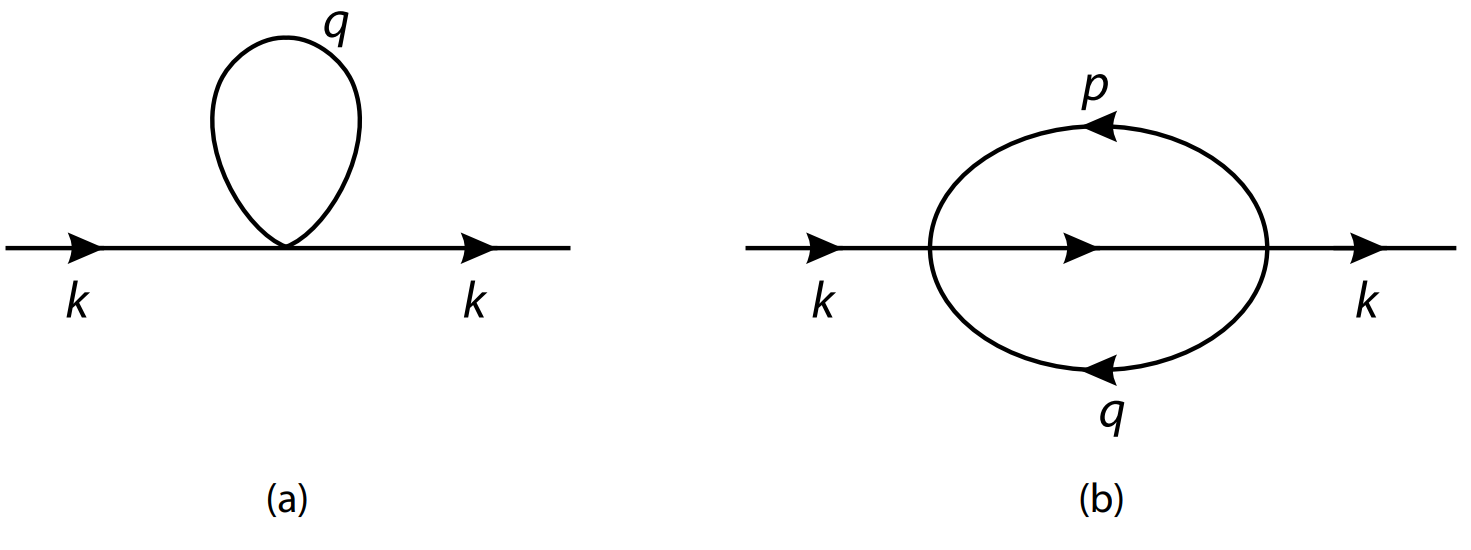
\includegraphics[scale=0.3]{mesons-phi-4}
\end{figure}

The amplitude associated with the first diagram has the form
\begin{align}
\mathcal{M}_1 \propto -i\lambda \int^\Lambda \f{d^4q}{(2\pi)^4}  \f{i}{q^2 - m^2 + i\epsilon}.
\end{align}
since there is one loop of variable momentum $q$. Because we are integrating over four dimensions of $q$ and taking away two dimensions of $q$, we get that this amplitude depends \textit{quadratically} on the cutoff $\Lambda$, but not on $k^2$. \\

On the other hand, the second diagram has a double integral because there are two variable momenta. There are two vertices and three internal lines, so
\begin{align}
\mathcal{M}_2 \propto (-i\lambda)^2 \iint^\Lambda \f{d^4p}{(2\pi)^4}\f{d^4q}{(2\pi)^4} \f{i}{p^2 - m^2 + i\epsilon} \f{i}{q^2 - m^2  + i\epsilon} \f{i}{(p+q+k)^2 - m^2  + i\epsilon}.
\end{align}
We see that we are integrating over 8 total dimensions of momentum, but taking away 6, so this integral depends quadratically on the cutoff $\Lambda$ as well. \\

We also notice that this integral is a function of $k^2$. So (by Lorentz invariance) we can expand it has the series
\begin{align}
D + Ek^2 + FK^4 + \dots
\end{align}
$D$ must have the same dimension as the integral, so it depends quadratically on $\Lambda$. $E$ can be obtained by differentiating with respect to $k$ twice. This decreases the power of $q,p$ in the integrand by 2 (since the power 2 now becomes 4) and so $E$ depends logarithmically on $\Lambda$ (the integral now looks like $\int d^8x\,1/x^8$). Similarly, we can reason that $F$ looks like the integral $\int d^8x\,1/x^10$ since we need to differentiate with respect to $k$ 4 times, increasing the power of $q,p$ in the exponential by $4$. All this means that $F$ converges and is cutoff-independent. Therefore, we know that $F$ and higher order terms of $k^2$ converge and are $\Lambda$-independent as well. We, then, don't have to worry about them.\\

With this, $\mathcal{M}_2$ is both quadratically and logarithmically cutoff-dependent. Now, suppose we do a \textbf{mass renormalization} by shifting the energy-momentum-mass:
\begin{align}
\f{1}{k^2 - m^2} \to \f{1}{(1+b)k^2 - (m^2 - a)}.
\end{align} 
Obviously the pole in $k^2$ is now shifted to 
\begin{align}
\boxed{m^2_P \equiv m^2 + \delta m^2 \equiv (m^2 - a)(1+b)^{-1}}
\end{align}
We refer to this as the \textbf{physical mass}. With this, we can write the propagator (in momentum space of course) as
\begin{align}
\boxed{\f{1}{k^2 - m^2} \to \f{(1+b)^{-1}}{k^2 - m^2_P}}
\end{align}


Notice here that the residue of the pole in this propagator is no longer 1 but $(1+b)^{-1}$. What is this shift in residue? \\

We note that the coefficient of $k^2$ in $1/\D(k)$ is identically 1 \textit{because} the coefficient of $(1/2)(\p \phi)^2$ is identically 1 in the Lagrangian density. Let's elaborate a little bit. Recall that the spacetime propagator is defined as the \textit{inverse} of the operator $(\square + m^2)$. It follows from here and some properties of Gaussian integrals that the propagator in momentum space has the form $1/(k^2 - m^2)$. This is essentially the derivation we did very early on. So, we see that there is certainly no guarantee that with higher order corrections included the coefficient of $(1/2)(\p \phi)^2$ in an effective $\lag$, say $\lag_{\text{eff}}$ will stay at 1. \\

In fact, by inspection, the coefficient is shifted from 1 to $(1+b)$. This is called \textbf{wavefunction renormalization}, or \textbf{field renormalization}. 






\subsubsection{Physical Perturbation Theory}

The physical perturbation theory is given by
\begin{align}
\boxed{ \lag = \f{1}{2}(\p \phi)^2 + \f{1}{2}m^2 \phi^2 - \f{\lambda_P}{4!}\phi^4 + A(\p \phi)^2 + B\phi^2 + C\phi^4.} 
\end{align}


This theory basically says for each order of $\phi$ in the regular Lagrangian, there is a perturbative term $A$, $B$, or $C$ of the same order the perturbative Lagrangian. This perturbative Lagrangian also carries the physical coupling constant $\lambda_P$ instead of the theoretical $\lambda$. \\



Here's how the theory works: The Feynman rules are as before, but with the crucial different that  the coupling constant is $\lambda_P$, and the propagator has the form
\begin{align}
\f{i}{k^2 - m_P^2 + i\epsilon},
\end{align}
where the physical mass is used instead. The last three terms with coefficients $A$, $B$, and $C$ are called \textbf{counterterms}. These coefficients are determined \textit{iteratively} as we go to higher and higher order in perturbation theory. These perturbations are represented as crosses in Feynman diagrams:
\begin{figure}[!htb]
	\centering
	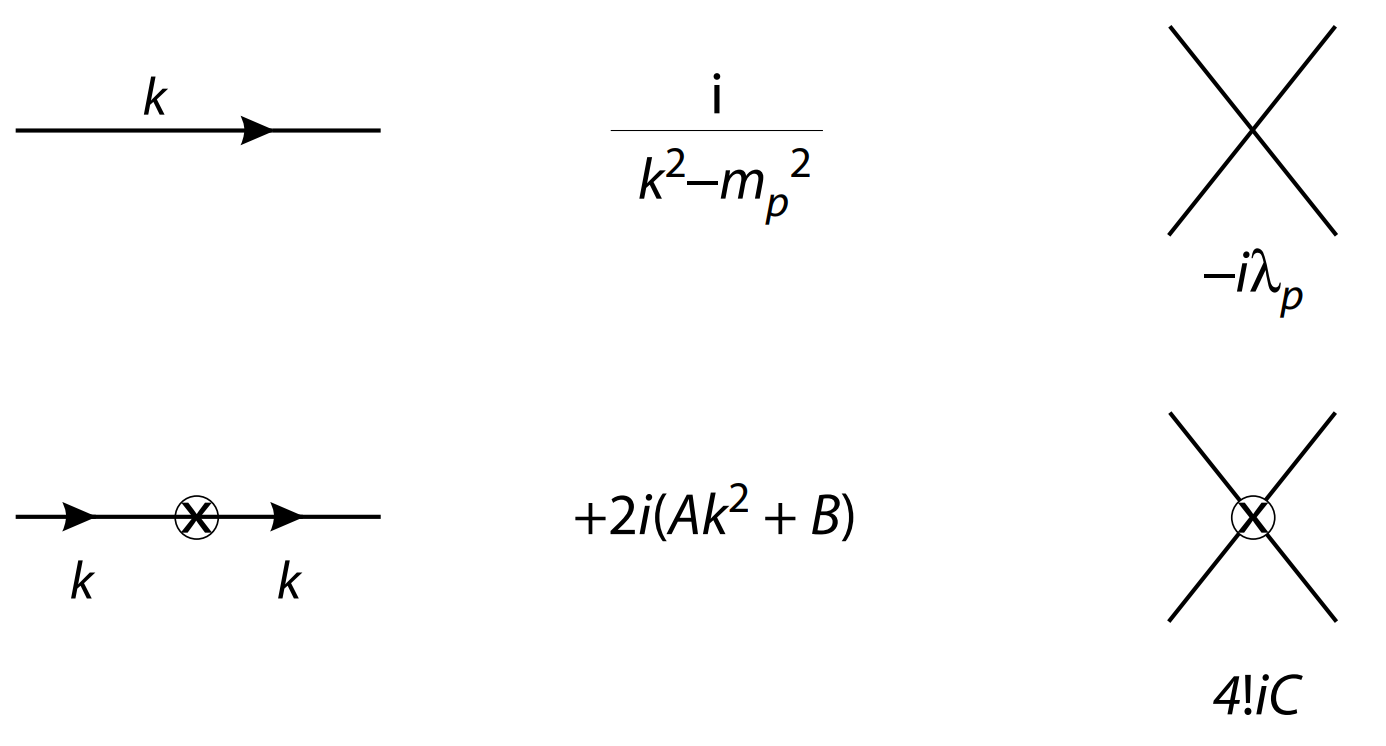
\includegraphics[scale=0.2]{crosses}
\end{figure}\\

We note that all momenta are integrated up to cutoff. \\

The coefficients $A$, $B$, $C$ are determined iteratively as follows. Suppose they are determined up to order $\lambda_P^N$. Let these values be $A_N$, $B_N$, and $C_N$. We then draw all diagrams that appear in order $\lambda_P^{N+1}$. We determine $A_{N+1}$, $B_{N+1}$, and $C_{N+1}$ by requiring that the propagator calculated to the order $\lambda^{N+1}_{P}$ has a pole at $m_p$ with a residue equal to 1, and that the meson=meson scattering amplitude evaluated at some specified values of the kinematic variables has the value $-i\lambda_P$. We note that there are exactly 3 conditions to determine the these three unknown coefficients.










\subsubsection{Degree of Divergence - Power Counting}




\noindent \textbf{Definition:} A diagram is said to have a superficial degree of divergence $D$ if it diverges as $\Lambda^D$. A logarithmic divergence $\log \Lambda$ counts as $D=0$. \qed \\

\noindent \textbf{$\phi$-Theorem:} For a diagram with $B_E$ external $\phi$ lines, the degree of divergence is given by
\begin{align}
\boxed{D = 4 - B_E}
\end{align}\qed \\


\noindent \textit{Proof by Zee:} The proof of this theorem follows from simple power counting. In addition to $B_E$ and $D$, let us define $B_I$ as the number of internal lines, $V$ as the number of vertices (where 4 lines meet), and $L$ as the number of loops. \\

The number of loops is just the number of $\int d^4k/(2\pi)^4$ that we have to do, i.e., it is the number of \textit{independent} internal momenta. Each internal line carries with it a momentum to be integrated over, so we seem to have $B_I$ integrals to do. However, the actual number of integrals to be done to reduced by the momentum conservation delta function associated with the vertices, one to each vertex. By assumption, there are $V$ delta functions, with one of them is associated with the conservation momentum of the entire diagram. It follows that the number of loops is
\begin{align}
L = B_I - (V - 1).
\end{align}


Now, for each vertex, there are four lines. Each external line comes out of one vertex. Each internal line connects two vertices. Thus we have
\begin{align}
4V = B_E + 2B_I.
\end{align}

Finally, for each loop there is a $\int d^k$ while for each internal line there is a $i/(k^2 -m^2 + i\epsilon)$, bringing the powers of momentum down by $2$. So,
\begin{align}
D = 4L - 2B_I.
\end{align}
Putting these relationship together, we obtain
\begin{align}
{D = 4- B_E}
\end{align}
as desired. \qed\\


\noindent \textit{Proof by Me:} I find my proof more intuitive. But I'm of course biased. \underline{To show:}
\begin{align}
D = 4 - B_E
\end{align}
where $D$ is the degree of divergence and $B_E$ is the number of external lines. Well, we know that the number $D$, or the number of divergence is equal to the total number of momentum dimensions in the integral measure, minus the total number of momentum dimensions in the denominator of the integrand, which is a product of propagators. In general, the scattering amplitude integral as the form
\begin{align}
\int \dots \int d^4 p_1 \dots d^4 p_n \lc \f{i}{k^2} \rc^{n'}. 
\end{align} 

So we first have
\begin{align}
D = 4n - 2n'.
\end{align}

Now, what are $n$ and $n'$? $n$ is the total number of integrals, which is equal to the number of ``momentum unknowns'' or ``internal momentum variables'' in a Feynman diagram. This number is completely determined by the number of vertices $V$ and internal lines $B_I$. If we associate to each internal line a variable momentum then we have $B_I$ variables to integrate over, but for each vertex there are two internal lines going out/in to it, so the number of variables is reduced by $V-1$. Note that we only consider internal lines going either in or out of a vertex to avoid double-counting. Thus we have 
\begin{align}
{\#} \text{ integrals } = B_I - (V - 1).
\end{align}

Next, $n'$ is the number of propagators, which is identically the number of internal lines $B_I$. So, 
\begin{align}
D = 4(B_I - (V - 1)) - 2B_I = 2(2 + B_I - 2V).
\end{align}
Okay, but we often know the number of external lines $B_E$, and also know that the total number of lines is 4 times the number of vertices (4 lines per vertex) minus the number of internal lines $B_I$ (accounting for double counting), so
\begin{align}
B_E + B_I = 4V - B_I \iff 2(2 + B - 2V) = 4 - 2B_E. 
\end{align}
Therefore,
\begin{align}
D = 4 - B_E.
\end{align}
\qed\\
















\textbf{Example.} Consider the attached diagram
\begin{figure}[!htb]
	\centering
	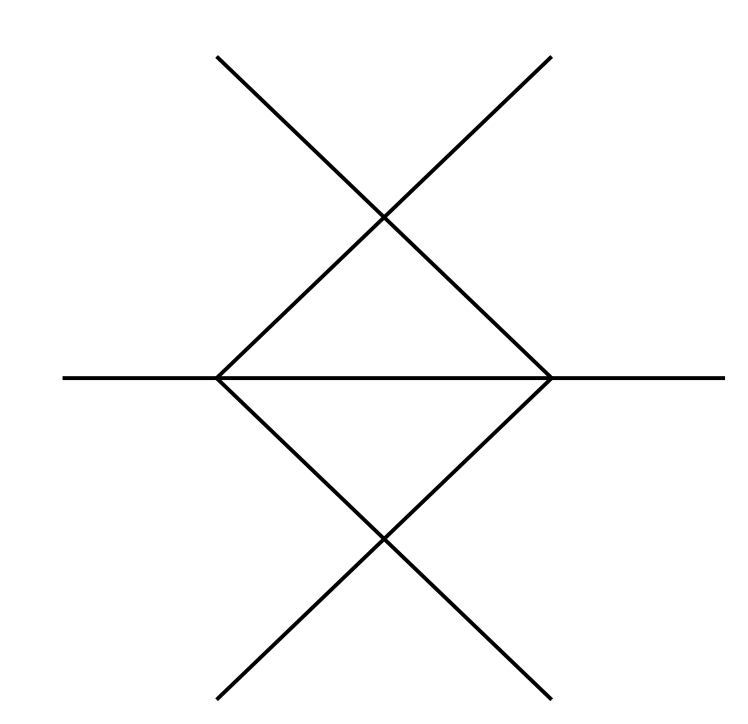
\includegraphics[scale=0.3]{div-count}
\end{figure}\\


By inspection, we have $B_E = 6$. So the theorem says $D = -2$. But we can also verify that this is true. Consider particles coming in from below. Then we have only 2 unknown variable momenta (since the momentum on the internal line in the middle is completely determined by the outgoing momenta and two variable momenta directly above and below). This means we integrate over 8 dimensions of momentum, while carrying 5 propagators, each with $-2$ dimensions of momentum. This means the degree of divergence is $8 - 10 = -2$. So things work as expected.






\subsubsection{Degree of Divergence with Fermions}



The theorem is modified for a different kind of particles. In this case, we have fermions instead of mesons like last time. \\

Consider the following Lagrangian for fermions, called the Yukawa theory
\begin{align}
\lag = \bar{\psi}(i\gamma^\mu \p_\mu - m_P)\psi + \f{1}{2}[(\p \phi)^2 - \mu^2_P \phi^2] - \lambda_P \phi^4 + f_P \phi \bar{\psi}\psi.
\end{align}


Here we have $F_I$ and $F_E$ as the number of internal and external lines as before, but there are two kinds of coupling: $\lambda$ and $f$. Also recall that $[\phi] = 1$ and $[\psi] = 3/2$. We now want to express $D$ in terms of external lines: bosonic external lines $B_E$ and fermionic external lines $F_E$. \\


It turns out that 
\begin{align}
\boxed{D = 4 - B_E - \f{3}{2}F_E}
\end{align}
So the degree of divergence for this theory has an extra dependence on the number of external fermionic lines. \\

To prove this, we will need to know what the fermion propagators are, but since we haven't discussed fermionic propagator up to this point I will present the proof later in this section. However, we can get a feel for why this holds by looking at some Feynman diagrams with fermions and photons. First, we have that vertex amplitudes are assigned as 
\begin{figure}[!htb]
	\centering
	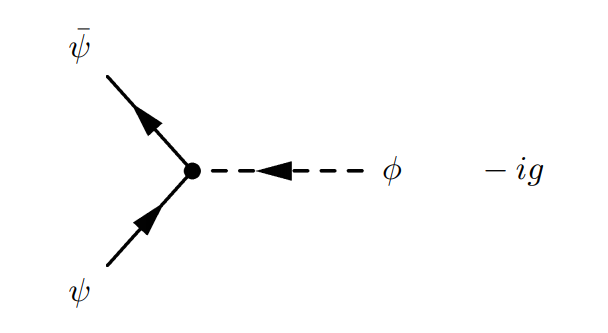
\includegraphics[scale=0.4]{fermi}
\end{figure}\\

With this, some simple Feynman diagrams with no loops look  like
\begin{figure}[!htb]
	\centering
	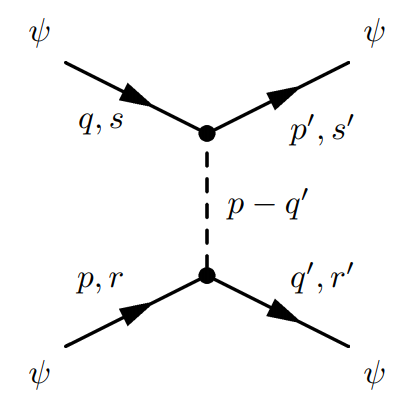
\includegraphics[scale=0.4]{fermi-diagram}
\end{figure}\\

or (with photon lines)
\begin{figure}[!htb]
	\centering
	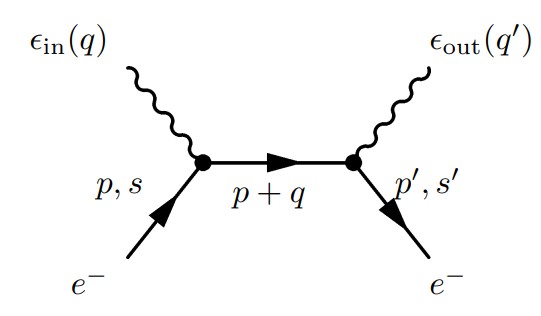
\includegraphics[scale=0.4]{compton}
	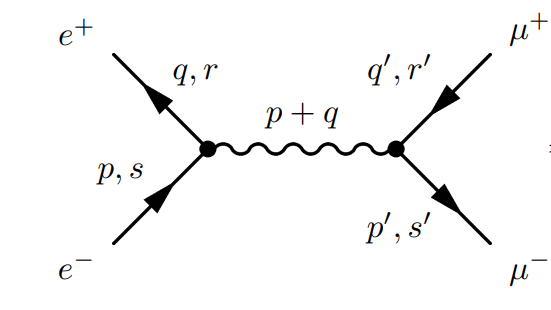
\includegraphics[scale=0.4]{fermi-gen}
\end{figure}\\













\textit{Proof:} Here we show that in fact in Yukawa theory
\begin{align}
D = 4 - B_E - \f{3}{2}F_E.
\end{align}  
The number of loop integrals is given by the number of independent four-momenta in a given diagram. Each propagator has its own four-momentum,
1 while each vertex enforces four-momentum conservation. However, there
always remains one overall four-momentum conservation of the diagram.
Hence,
\begin{align}
L = P_f + P_s - V_Y + 1
\end{align}
where $L$ is the number of loop integrals, $P_f$, $P_s$ the number of fermion or scalar
propagators, respectively, and $V_Y$ the number of Yukawa vertices. Since each
Yukawa vertex comes with two fermion lines and one scalar line,
\begin{align}
V_Y = \f{1}{2}(2P_f + N_f) = 2P_s + N_s.
\end{align}
Here, $N_f$, $N_s$ are the number of external fermion or scalar lines, respectively.
Each propagator is counted twice as it connects two vertices, while an external line connects to only one vertex. The superficial degrees of divergence is
\begin{align}
D = 4L - P_f - P_s.
\end{align}
Eliminating $V_Y$, $L$, $P_f$, $P_s$ from the above equations, we find
\begin{align}
{L = 4 - N_s - \f{3}{2}N_f}.
\end{align}


(to be continued)\\








Note: \textit{This proof is collected from Hitoshi's notes. }





\textbf{Remark 1:} We notice that both this result and the result from last section are independent of the number of vertices. This means for a given number of external lines, no matter to what order of perturbation theory we go, the superficial degree of divergence remains the same. \\

\textbf{Remark 2:} We also notice that the leading coefficient of $B_E$ and $F_E$ correspond to the dimension of the respective fields: $[\phi] = 1$, and $[\psi] = 3/2$.\\








\subsubsection{Nonrenormalizable field theories}


















\newpage



\subsection{Gauge Invariance: A Photon Can Find No Rest}



\newpage


\subsection{Field Theory without Relativity}


\newpage


\subsection{The Magnetic Moment of the Electron}



\newpage


\subsection{Polarizing the Vacuum and Renormalizing the Charge}

\newpage


\subsection{Becoming Imaginary and Conserving Probability}


































































												










































\newpage






























\chapter{QUANTUM OPTICS}

\newpage


\section{Quantization of the Electromagnetic Field}

\subsection{Quantization of a Single-mode Field}

Consider the following simple yet important scenario: a radiation field confined to a one-dimensional cavity along the $z$-axis with perfectly conducting walls at $z=0$ and $z=L$. 
\begin{figure}[!htb]
	\centering
	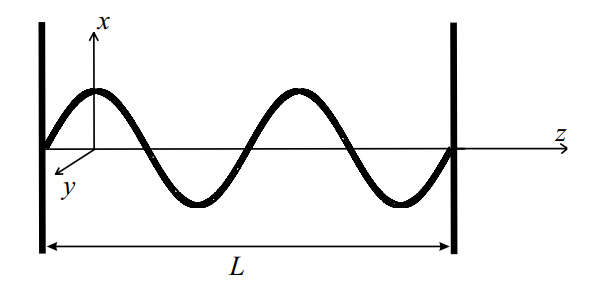
\includegraphics[scale=0.5]{em}
\end{figure}


Suppose that the field is a standing wave which vanishes on the boundary and is polarized in the $x$-direction. We also assume there is no source of radiation such as a charge or a current. The electric field then can be written as
\begin{align}
\mathbf{E}(\mathbf{r},t) = \mathbf{e}_xE_x(z,t)
\end{align}
where $\mathbf{e}_x$ is the polarization vector. The Maxwell's equations without source are
\begin{align}
\curl{\mathbf{E}} &= -\f{\p \mathbf{B}}{\p t}\\
\curl{\mathbf{B}} &= \mu_0\epsilon_0\f{\p \mathbf{E}}{\p t}\\
\div{\mathbf{E}} &= 0\\
\div{\mathbf{B}} &= 0.
\end{align}

A single-mode field satisfying Maxwell’s equations and the boundary conditions is given by
\begin{align}
E_x(z,t) = \lp \f{2\omega^2}{V\epsilon_0} \rp^{1/2} q(t)\sin(kz).
\end{align}
$\omega$ is the frequency, $k = \omega/c$ is the wavenumber. The allowed frequencies are
\begin{align}
\omega_m = c\f{m \pi}{L},\hspace{0.5cm}  =1,2,\dots
\end{align} 
$V$ is the effective volume of the cavity and $q(t)$ is the time-dependent factor having the dimension of length. The magnetic field, from the second Maxwell equation, is
\begin{align}
\mathbf{B}(\mathbf{r},t) = \mathbf{e}_yB_y(z,t)
\end{align}
where
\begin{align}
B_y(z,t) = \lp \f{\mu_0\epsilon_0}{k} \rp\lp \f{2\omega^2}{V\epsilon_0} \rp^{1/2}\dot{q}(t)\cos(kz).
\end{align}
It will become clear that $q(t)$ plays the role of canonical position, and $\dot{q}(t) = p(t)$ plays the role of canonical momentum. The classical field energy (or the Hamiltonian $\ham$) of this single-mode field is then given by
\begin{align}
\ham &= \f{1}{2}\int\,dV \lb \epsilon_0 \mathbf{E}^2(\mathbf{r},t) + \f{1}{\mu_0}\mathbf{B}^2(\mathbf{r},t) \rb\\
&= \f{1}{2}\int\,dV \lb \epsilon_0 E^2_x(z,t) + \f{1}{\mu_0}B_y^2(z,t) \rb
\end{align}
It turns out that (for $p(t) = \dot{q}(t)$), we have
\begin{align}
\boxed{\ham = \f{1}{2}\lp p^2 + \omega^2q^2 \rp}
\end{align} 
Now, we notice that we have the canonical variables $q$ and $p$. When we promote these variables to operators (so we can quantize the fields), these operators must satisfy the canonical commutation relation
\begin{align}
[\hat{q}, \hat{p}] = i\hbar \hat{\Id}.
\end{align}



We rewrite the fields and the Hamiltonian as operators:
\begin{align}
\hat{E}_x(z,t) &= \lp \f{2\omega^2}{V\epsilon_0} \rp^{1/2} \hat{q}(t)\sin(kz)\\
\hat{B}_y(z,t) &= \lp \f{\mu_0\epsilon_0}{k} \rp\lp \f{2\omega^2}{V\epsilon_0} \rp^{1/2}\hat{p}(t)\cos(kz).\\
\hat{\ham} &= \f{1}{2}\lp \hat{p}^2 + \omega^2\hat{q}^2 \rp.
\end{align}
The operators $\hat{q}$ and $\hat{p}$ correspond to observables because they are Hermitian. We can also introduce creation ($\hat{a}^\dagger$) and annihilation ($\hat{a}$) operators through combining $\hat{q}$ and $\hat{p}$:
\begin{align}
\hat{a} &= (2\hbar\omega)^{-1/2}(\omega\hat{q} + i\hat{p})\\
\hat{a}^\dagger &= (2\hbar\omega)^{-1/2}(\omega\hat{q} - i\hat{p})
\end{align}
It is easy to show that the electric and magnetic field operators then become
\begin{align}
\hat{E}_x(z,t) &= \mathcal{E}_0(\hat{a} + \hat{a}^\dagger)\sin(kz)\\
\hat{B}_y(z,t) &= \mathcal{B}_0\f{1}{i}(\hat{a} - \hat{a}^\dagger)\cos(kz)
\end{align}
where
\begin{align}
\mathcal{E}_0 = \sqrt{\f{\hbar\omega}{\epsilon_0 V}}, \hspace{0.5cm}
\mathcal{B}_0 = \lp\f{\mu_0}{k}\rp\sqrt{\f{\epsilon_0\hbar\omega^3}{V}}
\end{align}
represents respectively the electric and magnetic field ``per photon.'' We notice that
\begin{align}
[\hat{a}, \hat{a}^\dagger] = \hat{\Id}
\end{align}
so the Hamiltonian takes the form
\begin{align}
\boxed{\hat{\ham} = \hbar\omega\lp \hat{a}^\dagger\hat{a} + \f{1}{2} \rp}
\end{align}

Now, what is the time dependent of these new operators? For an arbitrary operator $\hat{O}$, Heisenberg equation reads
\begin{align}
\f{d\hat{O}}{dt} = \f{i}{\hbar}[\hat{H},\hat{O}].
\end{align}
For the annihilation operator, this becomes
\begin{align}
\f{d\hat{a}}{dt} = \f{i}{\hbar}\lb \hbar\omega\lp \hat{a}^\dagger\hat{a} + \f{1}{2} \rp, \hat{a} \rb = -i\omega \hat{a}.
\end{align}
Thus,
\begin{align}
\boxed{\hat{a}(t) = \hat{a}(0)e^{i\omega t}}
\end{align}
Similarly for the creation operator, we have
\begin{align}
\boxed{\hat{a}^\dagger(t) = \hat{a}^\dagger(0) e^{i\omega t}}
\end{align}

Now, let $\ket{n}$ denote an energy eigenstate of the single mode field corresponding to energy $E_n$, then 
\begin{align}
\hat{\ham}\ket{n} = \hbar\omega\lp \hat{a}^\dagger\hat{a} + \f{1}{2} \rp\ket{n} = E_n\ket{n}.
\end{align}
Applying the creation operator $\hat{a}^\dagger$ from the left we have
\begin{align}
\hbar\omega\lp \hat{a}^\dagger\hat{a}^\dagger\hat{a} + \f{1}{2}\hat{a}^\dagger \rp\ket{n} = E_n\hat{a}^\dagger\ket{n}.
\end{align}
Using the commutation relation, we can write 
\begin{align}
\hat{a}\hat{a}^\dagger = \hat{\Id} + \hat{a}^\dagger\hat{a}.
\end{align}
Thus,
\begin{align}
E_n\hat{a}^\dagger\ket{n} &= \hbar\omega\lp \hat{a}^\dagger[-\hat{\Id} + \hat{a}\hat{a}^\dagger] + \f{1}{2}\hat{a}^\dagger \rp\ket{n}\\
&= \hbar\omega\lp -\hat{a}^\dagger + \hat{a}^\dagger\hat{a}\hat{a}^\dagger + \f{1}{2}\hat{a}^\dagger \rp\ket{n}\\
&= \hbar\omega\lp -\hat{\Id} + \hat{a}^\dagger\hat{a} + \f{1}{2}  \rp\hat{a}^\dagger\ket{n}.
\end{align}
This says we have a new eigen-equation:
\begin{align}
(E_n + \hbar\omega) \hat{a}^\dagger\ket{n} = \hbar\omega\lp \hat{a}^\dagger\hat{a} + \f{1}{2} \rp\hat{a}^\dagger\ket{n}
\end{align}
or equivalently,
\begin{align}
\boxed{\hat{H}\lb\hat{a}^\dagger\ket{n}\rb = (E_n + \hbar\omega)\lb\hat{a}^\dagger\ket{n}\rb}
\end{align}
This is the eigenvalue problem for the eigenstate $\hat{a}^\dagger\ket{n}$ with the energy eigenvalue $E_n + \hbar\omega$. It is clear now why $\hat{a}^\dagger$ is called the creation operator: it creates a ``quantum'' energy $\hbar\omega$. On the other hand, we can also show that
\begin{align}
\boxed{\hat{H}\lb\hat{a}\ket{n}\rb = (E_n - \hbar\omega)\lb\hat{a}\ket{n}\rb} 
\end{align}
It is clear that the operator $\hat{a}$ annihilates a quantum of energy. Now, because for the least energetic eigenstate
\begin{align}
\hat{a}\ket{0} = 0,
\end{align}
the Hamiltonian of the annihilation of the least energetic eigenstate is 
\begin{align}
\hat{\ham}\lb \hat{a}\ket{0} \rb  = (E_0 - \hbar\omega)\lb \hat{a}\ket{0}\rb = 0.
\end{align}
Therefore,
\begin{align}
\hat{\ham}\ket{0} = \hbar\omega\lp \hat{a}^\dagger\hat{a} + \f{1}{2}\rp\ket{0} = \f{1}{2}\hbar\omega\ket{0} = E_0\ket{0}.
\end{align}
Or equivalently, the zero-point energy is 
\begin{align}
E_0 = \hbar\omega
\end{align}
and the energy eigenvalues $E_{n+1} = E_n + \hbar\omega$ are
\begin{align}
\boxed{E_n = \hbar\lp n + \f{1}{2}\rp}
\end{align}
Note that this is just like the energy levels for the harmonic oscillator in an infinite well. Now, we observe that
\begin{align}
\hat{\ham}\ket{n} = \hbar\omega\lp \hat{a}^\dagger\hat{a} + \f{1}{2}\rp \ket{n} = E_n\ket{n} = \hbar\omega\lp n + \f{1}{2} \rp\ket{n},
\end{align}
i.e.,
\begin{align}
\hat{a}^\dagger\hat{a}\ket{n} = n\ket{n}.
\end{align}
It makes sense to call $\hat{a}^\dagger\hat{a}$ the ``number operator'' $\hat{n}$, so that 
\begin{align}
\hat{n}\ket{n} = n\ket{n}.
\end{align}
Next, the eigenstates must be normalized according to $\braket{n} = 1$. For the state $\hat{a}\ket{n}$ we have
\begin{align}
\hat{a}\ket{n} = c_n\ket{n-1}.
\end{align}
Taking the inner product with itself we have
\begin{align}
\lp\bra{n}\hat{a}^\dagger\rp\lp\hat{a}\ket{n}\rp &= \bra{n}\hat{a}^\dagger\hat{a}\ket{n}\\
&= \bra{n}\hat{n}\ket{n}\\
&= n\braket{n}\\
&= \bra{n-1}c_n^*c_n\ket{n-1}.
\end{align}
This says $n = \abs{c_n}^2$. So we have
\begin{align}
\boxed{\hat{a}\ket{n} = \sqrt{n}\ket{n-1}}
\end{align}
Similarly, 
\begin{align}
\boxed{\hat{a}^\dagger\ket{n} = \sqrt{n+1}\ket{n+1}}
\end{align}
This says that $\ket{n}$ can be generated from the $\ket{0}$ state by applying the creation operator $\hat{a}^\dagger$ appropriately many times with the appropriate normalization:
\begin{align}
\boxed{\ket{n} = \f{{\lp\hat{a}^\dagger\rp}^n}{\sqrt{n!}}\ket{0}}
\end{align}


Next, because the eigenstates are orthonormal ($\braket{n'}{n} = \delta_{n'n}$ and $\braket{n}=1$) and form a complete set, i.e.,
\begin{align}
\sum^\infty_{n=0}\ket{n}\bra{n} = 1,
\end{align} 
the only non-vanishing matrix elements of the annihilation and creation operators are
\begin{align}
&\bra{n-1}\hat{a}\ket{n} = \sqrt{n}\braket{n-1} = \sqrt{n} \\
&\bra{n+1}\hat{a}^\dagger\ket{n} = \sqrt{n+1}\braket{n+1} = \sqrt{n+1}
\end{align}



\subsection{Quantum Fluctuations of a Single-mode Field}
Recall the electric field operator
\begin{align}
\hat{E}_x(z,t) &= \mathcal{E}_0(\hat{a} + \hat{a}^\dagger)\sin(kz).
\end{align}
The mean field is zero:
\begin{align}
\bra{n}\hat{E}_x(z,t)\ket{n} = \mathcal{E}_0\sin(kz)[\underbrace{\bra{n}\hat{a}\ket{n}}_{0} + \underbrace{\bra{n}\hat{a}^\dagger\ket{n}}_{0}] = 0
\end{align}
by orthonormality. However, the mean of the square of the field is not zero:
\begin{align}
\bra{n}\hat{E}^2_x(z,t)\ket{n} &= \mathcal{E}^2_0\sin^2(kz)\bra{n}{\lp\hat{a}^\dagger\rp}^2 + \hat{a}^2 + \hat{a}^\dagger\hat{a}+ \hat{a}\hat{a}^\dagger\ket{n}\\
&= \mathcal{E}^2_0\sin^2(kz)\bra{n} 2\hat{a}^\dagger\hat{a} + 1  \ket{n} \\
&= 2\mathcal{E}^2_0\sin^2(kz)\lp n + \f{1}{2}\rp.
\end{align}
So, the fluctuations in the field for the state $\ket{n}$ may be characterized by the variance
\begin{align}
\text{Var}[\hat{E}_x(z,t)] &= \text{E}[\hat{E}^2_x(z,t)] - \text{E}^2[\hat{E}_x(z,t)] \\ &= 2\mathcal{E}^2_0\sin^2(kz)\lp n + \f{1}{2}\rp.
\end{align}
And so the uncertainty of the field for the state $\ket{n}$ is
\begin{align}
\boxed{\sigma[\hat{E}_x(z,t)]= \sqrt{2\mathcal{E}_0}\sin(kz)\sqrt{n+ \f{1}{2}}}
\end{align}
Now, note that even at $n=0$, the field still has fluctuations. These are called ``vacuum fluctuations.'' Now the number states $\ket{n}$ are taken to represent a state of the field containing $n$ photons. Yet as we have seen, the average field is zero. This is all in accordance with the uncertainty principle because the number operator $\hat{n} = \hat{a}^\dagger\hat{a}$ does not commute with the electric field:
\begin{align}
[\hat{n}, \hat{E}_x] = \mathcal{E}_0 \sin(kz)(\hat{a}^\dagger - \hat{a}).
\end{align}
Thus $\hat{n}$ and $\hat{E}_x$ are complementary quantities for which their respective uncertainties obey the inequality
\begin{align}
\sigma[ n ]\cdot \sigma[ E_x ]\geq \f{1}{2}\mathcal{E}_0\abs{\sin(kz)}\abs{\langle \hat{a}^\dagger - \hat{a}\rangle}
\end{align}
This says that if the field is accurately known, then the number of photons in uncertain. 



\subsection{Quadrature Operators for a Single-mode Field}

When we explicitly include the time dependence of the electric field operator we have
\begin{align}
\hat{E}_x = \mathcal{E}_0 (\hat{a}e^{-\omega t} + \hat{a}^\dagger e^{i\omega t})\sin(kz)
\end{align}
where
\begin{align}
\hat{a}(0) \equiv \hat{a} \hspace{0.5cm} \hat{a}^\dagger(0) \equiv \hat{a}^\dagger.
\end{align}

Next, we define quadrature operators:
\begin{align}
&\hat{X}_1 = \f{1}{2}(\hat{a} + \hat{a}^\dagger)\\
&\hat{X}_2 = \f{1}{2i}(\hat{a} - \hat{a}^\dagger).
\end{align}
With these definitions, we rewrite the time-dependent electric field operator as
\begin{align}
\hat{E}_x(t) = 2\mathcal{E}_0\sin(kz)[\hat{X}_1 \cos(\omega t) + \hat{X}_2\sin(\omega t)].
\end{align}

We observe that $\hat{X}_1$ and $\hat{X}_2$ are associated with field amplitudes oscillating $\pi/2$ out of phase. Essentially, $\hat{X}_1$ and $\hat{X}_2$ are position and momentum operators, only scaled to be dimensionless. These operators satisfy the commutation relation
\begin{align}
[\hat{X}_1, \hat{X}_2] = \f{i}{2},
\end{align}
which one can easily check. Next, by definition we have
\begin{align}
\bra{n}\hat{X}_1\ket{n} = \bra{n}\hat{X}_2\ket{n} = 0.
\end{align}
However, 
\begin{align}
\bra{n}\hat{X}_1^2\ket{n} &= \f{1}{4}\bra{n} \hat{a}^2 + (\hat{a}^\dagger)^2 + \hat{a}^\dagger\hat{a} + \hat{a}\hat{a}^\dagger \ket{n}\\
&= \f{1}{4}\bra{n} 2\hat{a}^\dagger\hat{a} + 1 \ket{n}\\
&= \f{1}{4}(2n + 1).
\end{align}
Similarly, 
\begin{align}
\bra{n}\hat{X}_2^2\ket{n} = \f{1}{4}(2n + 1).
\end{align}
Thus for a number state, the uncertainties in both quadratures are the same and furthermore the vacuum state ($n = 0$) minimizes the uncertainty product since
\begin{align}
\text{Var}[\hat{X}_1] = \text{Var}[\hat{X}_2] = \f{1}{4}.
\end{align}

From this section, we learn that the quanta of the single-mode cavity field are the excitations of energy in discrete amounts of $\hbar\omega$. These quantas (or photons) are not localized particles but rather are spread out over the entire mode volume. 

















\subsection{Multimode Fields}

Now we generalize our results for the single-mode field to multi-mode fields. We again assume that there is no source of radiation. Let the vector potential $\mathbf{A}(\mathbf{r},t)$ be given such that
\begin{align}\label{gauge}
\div{\mathbf{A}(\mathbf{r},t)} = 0.
\end{align}
The vector potential gives the electric and magnetic fields by
\begin{align}\label{EB}
\mathbf{E}(\mathbf{r},t) &= -\f{\p \mathbf{A}(\mathbf{r},t)}{\p t}\\
\mathbf{B}(\mathbf{r},t) &= \curl{\mathbf{A}(\mathbf{r},t)}.
\end{align}
The vector potential satisfies the wave equation
\begin{align}\label{waves}
\laplacian{\mathbf{A}(\mathbf{r},t)} - \f{1}{c^2}\f{\p^2 \mathbf{A}(\mathbf{r},t)}{\p t^2} = 0.
\end{align}

We now assume free space is a cubic cavity with perfectly reflecting walls of length $L$. We assume that $L \to \infty$, i.e., $L$ is much larger than the wavelength of the field. This allows us to impose boundary conditions:
\begin{align}
&e^{ik_x x} = e^{ik_x(x+L)}\\
&e^{ik_y x} = e^{ik_y(y+L)}\\
&e^{ik_z x} = e^{ik_z(z+L)}.
\end{align}
It follows that
\begin{align}
&k_x = \lp \f{2\pi}{L} \rp m_x, \hspace{0.5cm} m_x = 0, \pm 1, \pm 2, \dots\\
&k_y = \lp \f{2\pi}{L} \rp m_y, \hspace{0.5cm} m_y = 0, \pm 1, \pm 2, \dots\\
&k_z = \lp \f{2\pi}{L} \rp m_z, \hspace{0.5cm} m_z = 0, \pm 1, \pm 2, \dots
\end{align}
The wave vector is then
\begin{align}
\mathbf{k} = \f{2\pi }{L}\begin{bmatrix}
m_x\\m_y\\m_z
\end{bmatrix}.
\end{align}
The magnitude of this vector is related to the frequency $\omega_k$ according to $k = \omega_k / c$. A set of integers $(m_x , m_y , m_z)$ specifies a normal mode of the field (apart from polarization), the number of modes being infinite but denumerable. The total number of modes in the intervals $\Delta m_x, \Delta m_y, \Delta m_z$ is
\begin{align}
\Delta m = \Delta m_x \Delta m_y \Delta m_z = 2\lp \f{L}{2\pi} \rp^3 \Delta k_x \Delta k_y \Delta k_z
\end{align}
where the factor of $2$ takes into account two independent modes of polarization. With the assumption that $L$ is very large compared to the wavelengths, this becomes
\begin{align}
dm = 2\lp \f{V}{8\pi^3} \rp d k_x d k_y d k_z.
\end{align}
In spherical coordinates, 
\begin{align}
\mathbf{k} = k(\sin\theta\cos\phi, \sin\theta\sin\phi, \cos\theta),
\end{align}
and 
\begin{align}
dm = 2\lp \f{V}{8\pi^3} \rp k^2 \, dk d\Omega
\end{align}
where
\begin{align}
d\Omega = \sin\theta \,d\theta d\phi.
\end{align}
With $k = \omega_k/c$,
\begin{align}
dm = 2\lp \f{V}{8\pi^3} \rp \f{\omega^2_k}{c^3} \, d\omega_k d\Omega.
\end{align}
Integrating over all solid angles gives $\int \,d\Omega = 4\pi$, so the number of modes in all directions from $k \to k + dk$ is 
\begin{align}
2\lp \f{V}{8\pi^3} \rp k^2 \cdot (4\pi) \, dk = V \f{k^2}{\pi^2}\,dk = V \rho_k \,dk
\end{align}
where $\rho_k = k^2/\pi^2$ and $\rho_k \,dk$ is the number of modes per unit volume. Integrating in the same fashion but with $\omega_k$ gives the number of modes in all directions from $\omega_k \to \omega_k + d\omega_k$:
\begin{align}
V \lp \f{\omega_k^2}{\pi^2 c^3} \rp\,d\omega_k = V \rho(\omega_k)\,d\omega_k
\end{align}
where now $\rho(\omega_k)$ is also the mode density. \\

The vector potential can be written as a superposition on plane waves in the form
\begin{align}
\mathbf{A}(\mathbf{r},t) = \sum_{\mathbf{k},s}\mathbf{e}_{\mathbf{k}s} \lb A_{\mathbf{k}s}(t)e^{i\mathbf{k}\cdot\mathbf{r}} + A_{\mathbf{k}s}^* e^{-i\mathbf{k}\cdot \mathbf{r}} \rb 
\end{align}
where $A_{\mathbf{k}s}$ is the complex amplitude of the field and $\mathbf{e}_{\mathbf{k}s}$ is a real polarization vector. The sum over $k$ simply means the sum over the set of integers $(m_x , m_y , m_z)$ and the sum over $s$ is the sum over the two independent polarizations. These polarizations must be orthogonal:
\begin{align}
\mathbf{e}_{\mathbf{k}s} \cdot \mathbf{e}_{\mathbf{k}s'} = 0
\end{align}
and the \textit{transversality} condition must be satisfied:
\begin{align}
\mathbf{k}\cdot\mathbf{e}_{\mathbf{k}s} = 0,
\end{align}
which is just says that the polarization is orthogonal to the propagation. The polarization vectors $\mathbf{e}_{\mathbf{k}1}$ and $\mathbf{e}_{\mathbf{k}2}$ form a right-handed system:
\begin{align}
\mathbf{e}_{\mathbf{k}1}\times \mathbf{e}_{\mathbf{k}2} = \f{\mathbf{k}}{\abs{\mathbf{k}}} = \mathbf{\kappa}.
\end{align}
In free space, we make the transition from ``discrete'' modes to a continuum of modes, thus the sum becomes an integral:
\begin{align}
\sum_{\mathbf{k}} \to \f{V}{\pi^2}\int k^2\,dk.
\end{align}
From \eqref{gauge} and \eqref{waves} and $\omega_k = kc$, we get
\begin{align}
\f{d^2 A_{\mathbf{k}s}}{dt^2} + \omega_k^2 A_{\mathbf{k}s} =0. 
\end{align}
The solution to this is of course
\begin{align}
A_{\mathbf{k}s}(t) = A_{\mathbf{k}s}(0)e^{-i\omega_k t} = A_{\mathbf{k}s}e^{-i\omega_k t}.
\end{align}
From this and \eqref{EB} we can derive the electric and magnetic fields:
\begin{align}
&\mathbf{E}(\mathbf{r},t) = i\sum_{\mathbf{k},s} \omega_k \mathbf{e}_{\mathbf{k}s} \lb A_{\mathbf{k}s}e^{i(\mathbf{k}\cdot\mathbf{r} - \omega_k t)} - A_{\mathbf{k}s}^* e^{-i(\mathbf{k}\cdot\mathbf{r} - \omega_k t)}\rb\\
&\mathbf{B}(\mathbf{r},t) = \f{i}{c}\sum_{\mathbf{k},s} \omega_k (\mathbf{\kappa} \times \hat{\mathbf{e}}_{\mathbf{k}s}) \lb A_{\mathbf{k}s}e^{i(\mathbf{k}\cdot\mathbf{r} - \omega_k t)} - A_{\mathbf{k}s}^* e^{-i(\mathbf{k}\cdot\mathbf{r} - \omega_k t)}\rb.
\end{align}
The electromagnetic Hamiltonian is given by
\begin{align}
\ham = \f{1}{2}\int_V \lp \epsilon_0 \mathbf{E}\cdot \mathbf{E} + \f{1}{\mu_0} \mathbf{B}\cdot\mathbf{B} \rp\,dV.
\end{align}
The periodic boundary conditions result in
\begin{align}
\int_0^L e^{\pm i k_x x}\,dx = \begin{cases}
L,\hspace{0.5cm} k_x = 0\\
0,\hspace{0.5cm} k_x \neq 0
\end{cases}
\end{align}
same for $y$ and $z$. Collectively we write this as
\begin{align}
\int_V e^{\pm i(\mathbf{k} - \mathbf{k}')\cdot\mathbf{r}} \, dV = \delta_{\mathbf{k}\mathbf{k}'}V.
\end{align}
So the contribution to the Hamiltonian from the electric field is
\begin{align}
\f{1}{2}\int_V \epsilon_0 \mathbf{E}\cdot\mathbf{E}\,dV = &\epsilon_0 V \sum_{\mathbf{k}s}\omega_k^2 A_{\mathbf{k}s}(t)A^*_{\mathbf{k}s}(t) \\
& - \underbrace{\f{1}{2}\epsilon_0 V\sum_{\mathbf{k}ss'}\omega^2_k \mathbf{e}_{\mathbf{k}s}\cdot \mathbf{e}_{-\mathbf{k}s'}\lb A_{\mathbf{k}s}(t)A_{\mathbf{k}s'}(t) + A^*_{\mathbf{k}s}(t)A^*_{-\mathbf{k}s'}(t) \rb}_R.
\end{align}
To obtain the magnetic contribution we use the identity
\begin{align}
(\mathbf{A}\times \mathbf{B})\cdot (\mathbf{C}\times \mathbf{D}) = (\mathbf{A}\cdot\mathbf{C})(\mathbf{B}\cdot \mathbf{D}) - (\mathbf{A}\cdot\mathbf{D})(\mathbf{B}\cdot\mathbf{C}).
\end{align}
This gives
\begin{align}
(\mathbf{\kappa}\times \mathbf{e}_{\mathbf{k}s})\cdot(\mathbf{\kappa}\times \mathbf{e}_{\mathbf{k}s'}) &= \delta_{ss'}\\
(\mathbf{\kappa}\times \mathbf{e}_{\mathbf{k}s})\cdot(-\mathbf{\kappa}\times \mathbf{e}_{-\mathbf{k}s'}) &= -\mathbf{e}_{\mathbf{k}s}\cdot \mathbf{e}_{-\mathbf{k}s'}.
\end{align}
With this we get the contribution from the magnetic field
\begin{align}
\f{1}{2}\int_V \f{1}{\mu_0}\mathbf{B}\cdot\mathbf{B}\,dV = &\epsilon_0 V \sum_{\mathbf{k}s}\omega^2_k A_{\mathbf{k}s}(t)A^*_{\mathbf{k}s}(t) + R.
\end{align}
Thus the Hamiltonian is
\begin{align}
\ham &= 2\epsilon_0 V \sum_{\mathbf{k}s} \omega^2_k A_{\mathbf{k}s}(t)A^*_{\mathbf{k}s}(t)\\
&= 2\epsilon_0 V \sum_{\mathbf{k}s} \omega^2_k A_{\mathbf{k}s}(0)e^{-i\omega_k t}A^*_{\mathbf{k}s}(0)e^{i\omega_k t}\\
&= 2\epsilon_0 V \sum_{\mathbf{k}s} \omega^2_k A_{\mathbf{k}s}A^*_{\mathbf{k}s}.
\end{align}
To quantize the field, the canonical variables $q_{\mathbf{k}s}$ and $p_{\mathbf{k}s}$ must be introduced:
\begin{align}
A_{\mathbf{k}s} &= \f{1}{2\omega_k \sqrt{\epsilon_0 V}}[\omega_k q_{\mathbf{k}s} + ip_{\mathbf{k}s}]\\
A^*_{\mathbf{k}s} &= \f{1}{2\omega_k \sqrt{\epsilon_0 V}}[\omega_k q_{\mathbf{k}s} - ip_{\mathbf{k}s}]
\end{align}
such that when we can re-write the Hamiltonian as
\begin{align}
\ham = \f{1}{2}\sum_{\mathbf{k}s} \lp p^2_{\mathbf{k}s} + \omega_k^2q_{\mathbf{k}s}^2\rp.
\end{align}

To quantize the field, we promote these canonical variables to operators:
\begin{align}
\boxed{\hat{\ham} = \f{1}{2}\sum_{\mathbf{k}s} \lp \hat{p}^2_{\mathbf{k}s} + \omega_k^2\hat{q}_{\mathbf{k}s}^2\rp}
\end{align}
where 
\begin{align}
\lb\hat{q}_{\mathbf{k}s}, \hat{q}_{\mathbf{k}'s'}\rb &= 0 = \lb\hat{p}_{\mathbf{k}s}, \hat{p}_{\mathbf{k}'s'}\rb \\
\lb\hat{q}_{\mathbf{k}s}, \hat{p}_{\mathbf{k}'s'}\rb &= i\hbar\delta_{\mathbf{kk}'}\delta_{ss'}.
\end{align}
The annihilation and creation operators are defined in a similar fashion as in the case of a single-mode field:
\begin{align}
\hat{a}_{\mathbf{k}s} &= (2\hbar\omega_k)^{-1/2}(\omega_k \hat{q}_{\mathbf{k}s} + i\hat{p}_{\mathbf{k}s})\\
\hat{a}^\dagger_{\mathbf{k}s} &= (2\hbar\omega_k)^{-1/2}(\omega_k \hat{q}_{\mathbf{k}s} - i\hat{p}_{\mathbf{k}s})
\end{align}
which satisfy
\begin{align}
\lb\hat{a}_{\mathbf{k}s}, \hat{a}_{\mathbf{k}'s'}\rb &= 0 = \lb\hat{a}^\dagger_{\mathbf{k}s}, \hat{a}^\dagger_{\mathbf{k}'s'}\rb\\
\lb \hat{a}_{\mathbf{k}s}, \hat{a}^\dagger_{\mathbf{k}'s'}  \rb &= \delta_{\mathbf{kk}'}\delta_{ss'}.
\end{align}
Finally, we define a similar operator for the mode $\mathbf{k}s$ as the ``number'' operator before
\begin{align}
\hat{n}_{\mathbf{k}s} = \hat{a}^\dagger_{\mathbf{k}s} \hat{a}_{\mathbf{k}s}.
\end{align}
With these, the Hamiltonian (operator) can be written as
\begin{align}
\hat{\ham} = \sum_{\mathbf{k}s}\hbar\omega_k \lp \hat{a}_{\mathbf{k}s}^\dagger\hat{a}_{\mathbf{k}s} + \f{1}{2} \rp = \sum_{\mathbf{k}s} \omega_k \lp \hat{n}_{\mathbf{k}s} +\f{1}{2} \rp.
\end{align}
For simplicity, we associate a $j^\text{th}$ mode with $\mathbf{k}_js_j$. We let
\begin{align}
\hat{a}_{\mathbf{k}_j s_j} &\equiv \hat{a}_j\\
\hat{a}^\dagger_{\mathbb{k}_j s_j} &\equiv \hat{a}^\dagger_j\\
\hat{n}_{\mathbf{k}_j s_j} &\equiv \hat{n}_j.
\end{align}
Now we can write the Hamiltonian as
\begin{align}
\boxed{\hat{\ham} = \sum_j \hbar\omega_j \lp \hat{n}_j + \f{1}{2} \rp}
\end{align}

A multimode photon number state is a (tensor) product of the number states $\ket{n_{\mathbf{k}s}} \equiv \ket{n_j}$ of all the modes which we write as
\begin{align}
\ket{n_1}\ket{n_2}\ket{n_3}\dots \equiv \ket{n_1n_2n_3\dots} = \ket{\{ n_j \}}.
\end{align}
This is an eigenstate of the Hamiltonian:
\begin{align}
\hat{\ham}\ket{\{ n_j \}} = E\ket{\{ n_j \}}.
\end{align}
We can show that energy eigenvalue is
\begin{align}
\boxed{E = \sum_j \hbar\omega_j \lp n_j + \f{1}{2} \rp}
\end{align}
Because the Hamiltonian is Hermitian (as always) the eigenstates are orthogonal:
\begin{align}
\bra{n_1n_2n_3\dots}\ket{n'_1n'_2n'_3\dots} = \delta_{n_1n'_1}\delta_{n_2n'_2}\delta_{n_3n'_3}\dots
\end{align}
The actions of the annihilation and creation operator are as expected and similar to what we have seen before:
\begin{align}
&\boxed{\textbf{Annihilation: } \hat{a}_j \ket{n_1,n_2,\dots,n_j,\dots} = \sqrt{n_j}\ket{n_1,n_2,\dots,n_j - 1,\dots}}\\
&\boxed{\textbf{Creation: } \hat{a}^\dagger_j \ket{n_1,n_2,\dots,n_j,\dots} = \sqrt{n_j + 1}\ket{n_1,n_2,\dots,n_j + 1,\dots}}
\end{align}


The vacuum multimode is denoted
\begin{align}
\ket{\{ 0 \}} = \ket{0_10_20_3\dots 0_j\dots}
\end{align}
for which
\begin{align}
\hat{a}_j \ket{\{ 0 \}} = 0 \hspace{0.5cm} \text{for all }j.
\end{align}
Once again, like in the single-mode case, a multimode number state can be generated by applying the creation operator. Any number state can be written as some creation operator applied to the multimode vacuum:
\begin{align}
\ket{\{ n_j \}} = \prod_{j} \f{(\hat{a}^\dagger_{j})^{n_j}}{\sqrt{n_j !}}\ket{\{ 0 \}}.
\end{align}

Now, we notice that the creation/annihilation operators $\hat{a}_{\mathbf{k}s}$/$\hat{a}^\dagger_{\mathbf{k}s}$ are very much like the vector potential amplitude $A_{\mathbf{k}s}$. Indeed, upon quantization of the field, the amplitudes can be promoted to operators as well:
\begin{align}
\hat{A}_{\mathbf{k}s} = \lp \f{\hbar}{2\omega_k \epsilon_0 V} \rp^{\f{1}{2}}\hat{a}_{\mathbf{k}s}.
\end{align}
With this, we are able to rewrite the vector potential, electric, and magnetic fields in terms of the creation and annihilation operators:
\begin{align}
&\hat{\mathbf{A}}(\mathbf{r},t) = \sum_{\mathbf{k}s}\lp\f{\hbar}{2\omega_k \epsilon_0 V}\rp^{\f{1}{2}} \mathbf{e}_{\mathbf{k}s} \lb \hat{a}_{\mathbf{k}s}e^{i(\mathbf{k}\cdot\mathbf{r} - \omega_k t)}
+ \hat{a}^\dagger_{\mathbf{k}s}e^{-i(\mathbf{k}\cdot\mathbf{r} - \omega_k t)}  \rb\\
&\hat{\mathbf{E}}(\mathbf{r},t) = i\sum_{\mathbf{k}s}\lp\f{\hbar\omega_k}{2\epsilon_0 V}\rp^{\f{1}{2}} \mathbf{e}_{\mathbf{k}s} \lb \hat{a}_{\mathbf{k}s}e^{i(\mathbf{k}\cdot\mathbf{r} - \omega_k t)}
- \hat{a}^\dagger_{\mathbf{k}s}e^{-i(\mathbf{k}\cdot\mathbf{r} - \omega_k t)}  \rb\\
&\hat{\mathbf{B}}(\mathbf{r},t) = \f{i}{c}\sum_{\mathbf{k}s} (\mathbf{\kappa} \times \mathbf{e}_{\mathbf{k}s})\lp\f{\hbar\omega_k}{2 \epsilon_0 V}\rp^{\f{1}{2}} \mathbf{e}_{\mathbf{k}s} \lb \hat{a}_{\mathbf{k}s}e^{i(\mathbf{k}\cdot\mathbf{r} - \omega_k t)}
- \hat{a}^\dagger_{\mathbf{k}s}e^{-i(\mathbf{k}\cdot\mathbf{r} - \omega_k t)}  \rb.
\end{align}



The annihilation and creation operators are to be understood as Heisenberg picture operators evaluated at $t=0$. The time-dependent annihilation operator for a free field is given by  
\begin{align}
\hat{a}_{\mathbf{k}s}(t) = \hat{a}_{\mathbf{k}s}(0)e^{-i\omega_k t}.
\end{align}
With this the electric field can be written as
\begin{align}
\hat{\mathbf{E}}(\mathbf{r},t) = i\sum_{\mathbf{k}s}\lp \f{\hbar\omega_k}{2\epsilon_0 V} \rp^{\f{1}{2}} \mathbf{e}_{\mathbf{k}s}   \lb \hat{a}_{\mathbf{k}s}(t)e^{i\mathbf{k}\cdot\mathbf{r}} - \hat{a}^\dagger_{\mathbf{k}s}(t)e^{-i\mathbf{k}\cdot\mathbf{r}} \rb.
\end{align}
where the $e^{\pm i \omega_k t}$ term is absorbed into the operator. Alternatively, the field can be written in a different form:
\begin{align}
\hat{\mathbf{E}}(\mathbf{r},t) = \hat{\mathbf{E}}^{(+)}(\mathbf{r},t) + \hat{\mathbf{E}}^{(-)}(\mathbf{r},t)
\end{align}
where
\begin{align}
\hat{\mathbf{E}}^{(+)}(\mathbf{r},t) = i\sum_{\mathbf{k}s}\lp \f{\hbar\omega_k}{2\epsilon_0 V} \rp^{\f{1}{2}}\mathbf{e}_{\mathbf{k}s}\hat{a}_{\mathbf{k}s}(t)e^{ i\mathbf{k}\cdot\mathbf{r}}.
\end{align}
Of course,
\begin{align}
\hat{\mathbf{E}}^{(+)}(\mathbf{r},t) = \lb \hat{\mathbf{E}}^{(-)}(\mathbf{r},t) \rb^\dagger.
\end{align}

Similar expressions can be obtained for the magnetic field. However, because the magnetic field is ``weaker'' than the electric field by a factor of $1/c$, we generally neglect the magnetic field in most matter-field interactions (as most interactions are through the electric dipole). $\hat{\mathbf{E}}^{(+)}(\mathbf{r},t)$ is called the \textit{positive frequency part} of the field as it contained all terms oscillate as $e^{-i\omega t}$ for $\omega > 0$. The opposite is for $\hat{\mathbf{E}}^{(-)}(\mathbf{r},t)$. We notice that $\hat{\mathbf{E}}^{(+)}(\mathbf{r},t)$ is a collective annihilation operator while the latter is a collective creation operator. \\

The last observation we make is the following. For a single-mode plane wave field the electric field is
\begin{align}
\hat{E}(\mathbf{r},t) = i\lp \f{\hbar\omega_k}{2\epsilon_0 V} \rp^{\f{1}{2}}\mathbf{e}_x\lb \hat{a} e^{i\mathbf{k}\cdot\mathbf{r} - i\omega t} - \hat{a}^\dagger e^{-i\mathbf{k}\cdot\mathbf{r} + i\omega t} \rb.
\end{align}
In most of quantum optics, the spatial variation of the field over the dimensions of the atomic system may be negligible, i.e., the length characteristic of the size of the atom is often much smaller than a typical wavelength:
\begin{align}
\f{\lambda}{2\pi} = \f{1}{\abs{k}} \gg \abs{\mathbf{r}_\text{atom}}.
\end{align}
With this, we can make an approximation:
\begin{align}
e^{\pm i\mathbf{k}\cdot\mathbf{r}} \approx 1 \pm i\mathbf{k}\cdot\mathbf{r}
\end{align}
which says we replace the exponential by unity for $\abs{\mathbf{r}}$ is negligible. Under this approximation, 
\begin{align}\label{dipoleE}
\boxed{\hat{\mathbf{E}}(\mathbf{r},t)  \approx \hat{\mathbf{E}}(t) = i \lp \f{\hbar\omega_k}{2\epsilon_0 V} \rp^{\f{1}{2}}\mathbf{e}_x \lb \hat{a}e^{-i\omega t} - \hat{a}^\dagger e^{i\omega t} \rb}
\end{align}
This is called the \textbf{``dipole'' approximation}. 




%\newpage
%
%\section{Coherent States}

\newpage

\section{Emission and Absorption of Radiation by Atoms}

\subsection{Atom-field interactions}
Suppose we have an atom in no external field. The Hamiltonian of an electron bound to this atom is given by
\begin{align}
\hat{\ham}_0 = \f{1}{2m}\hat{\mathbf{P}}^2 + V(r)
\end{align}
where $V(r)$ is the Coulomb interaction between the electron and nucleus and $r = \abs{\mathbf{r}}$ is the distance to the core. In the configuration space representation, 
\begin{align}
&\hat{\mathbf{P}} = -i \hbar \nabla\\
&\hat{\mathbf{r}}\ket{\mathbf{r}} = \mathbf{r}\ket{\mathbf{r}}.
\end{align}
The wave functions are given by
\begin{align}
\psi(\mathbf{r}) = \bra{\mathbf{r}}\ket{\psi}.
\end{align}
We assume that the energy eigenstates $\ket{k}$ of $\hat{\ham}_0$ satisfy the time-independent Schr\"{o}dinger equation:
\begin{align}
\hat{\ham}_0 \ket{\psi}_k^{(0)}(\mathbf{r}) = E_k \psi_k^{(0)}(\mathbf{r}) 
\end{align}
where 
\begin{align}
\bra{\mathbf{r}}\ket{k} = \psi_k^{(0)}(\mathbf{r})
\end{align}
are known. In the presence of external fields the Hamiltonian is modified to
\begin{align}
\hat{\ham}(\mathbf{r},t) = \f{1}{2m}\lb \hat{\mathbf{P}} + e\mathbf{A}(\mathbf{r} , t) \rb^2 - e\Phi(\mathbf{r},t) + V(r)
\end{align}
where $\mathbf{A}(\mathbf{r},t)$ and $\Phi(\mathbf{r},t)$ are the vector and scalar potentials, respectively, $-e$ is the electron charge. The electric and magnetic fields are given by
\begin{align}
&\mathbf{E}(\mathbf{r},t) = -\grad{\Phi(\mathbf{r},t)} - \f{\p \mathbf{A}(\mathbf{r},t)}{\p t}\\
&\mathbf{B}(\mathbf{r},t) = \curl{\mathbf{A}(\mathbf{r},t)}
\end{align}
which we can easily show to be invariant under the following gauge transformations
\begin{align}\label{gaug}
&\Phi'(\mathbf{r},t) = \Phi(\mathbf{r},t) - \f{\p \chi(\mathbf{r},t)}{\p t}\\
&\mathbf{A}'(\mathbf{r},t) = \mathbf{A}(\mathbf{r},t) + \grad{\chi(\mathbf{r},t)}.
\end{align}
The time-dependent Schr\"{o}dinger equation is
\begin{align}
\hat{\ham}(\mathbf{r},t)\psi(\mathbf{r},t) = i\hbar\f{\p \psi(\mathbf{r},t)}{\p t}.
\end{align}
To eventually simplify the form of the atom-field interaction, we define a unitary operator $\hat{R}$ such that
\begin{align}
\psi'(\mathbf{r},t) = \hat{R}\psi(\mathbf{r},t)
\end{align}
where
\begin{align}
\hat{\ham}' \psi'  = i\hbar \f{\p \psi'}{\p t}.
\end{align}
We can show that the new Hamiltonian relates to the old Hamiltonian as 
\begin{align}
\hat{\ham}' = \hat{R}\hat{\ham}\hat{R}^\dagger + i\hbar \f{\p \hat{R}}{\p t}\hat{R}^\dagger.
\end{align}
Our goal is to choose 
\begin{align}
\hat{R} = e^{-ie\chi(\mathbf{r},t)/\hbar},
\end{align}
so that with $\hat{\mathbf{P}}^2 = -i\hbar \nabla$:
\begin{align}
\hat{\ham}' =\f{1}{2m}\lb \hat{\mathbf{P}}^2 + e\mathbf{A}' \rb^2 - e\Phi' + V(r),
\end{align}
where the new vector and scalar potentials $\mathbf{A}'$ and $\Phi'$ depend on the gauge field $\chi$ as \eqref{gaug}. This form of the Hamiltonian is not desirable because of the interaction terms $\hat{\mathbf{P}} \cdot \mathbf{A}$ and $\mathbf{A}^2$. To remedy this, we can first make a definite choice of gauge, namely the Coulomb gauge, for which $\Phi = 0$ and $\div{\mathbf{A}} = 0$. Now with $\mathbf{A'} = \mathbf{A} + \grad{\chi}$ and $\Phi' = \Phi - \p \chi / \p t = - \p \chi / \p t$, the new Hamiltonian has the form
\begin{align}\label{newHam}
\hat{\ham}' = \f{1}{2m}\lb \hat{\mathbf{P}} + e\lp\mathbf{A} + \grad{\chi}\rp \rb^2 + e\f{\p \chi}{\p t} +V(r).
\end{align}
The vector potential $\mathbf{A}$ for no sources near the atom satisfies the wave equation
\begin{align}
\laplacian{\mathbf{A}} - \f{1}{c^2}\f{\p^2 \mathbf{A}}{\p t^2} = 0,
\end{align}
whose solution is simply a wave propagating wave
\begin{align}
\mathbf{A} = \mathbf{A}_0 e^{i(\mathbf{k}\cdot\mathbf{x} - \omega t)} + c.c.
\end{align}
where $\abs{\mathbf{k}} = 2\pi/\lambda$ is the wave vector of the radiation. For $\abs{\mathbf{r}}$ a typical atomic length ($10^{-10}$ m) and $\lambda$ of typical optical wavelengths ($10^{-7}$ m), the product $\mathbf{k}\cdot\mathbf{r} \ll 1$ so that over the extend of the atom $\mathbf{A}$ can be taken to be uniform, i.e.,
\begin{align}
\mathbf{A}(\mathbf{r},t) \approx \mathbf{A}(t).
\end{align} 
This is very much like the idea we discussed before regarding the electric field $\mathbf{E}$ in the quantization of the EM field. This is also called the \textbf{dipole approximation}. Now, the Hamiltonian in \eqref{newHam} has coupled terms, and we would like to remove $\nabla \chi$ from the coupling between itself and $\mathbf{A}$ and between $\mathbf{A}$ and $\hat{\mathbf{P}}$. One very good way to do this is finding $\chi$ such that
\begin{align}
\nabla \chi = - \mathbf{A}(\mathbf{r},t) \approx \mathbf{A}(t).
\end{align}
Such a $\chi(\mathbf{r},t)$ is
\begin{align}
\chi(\mathbf{r},t) = - \mathbf{A}(t)\cdot \mathbf{r}.
\end{align}
With this choice, we have (since $\nabla \mathbf{r} = \mathbf{1}$)
\begin{align}
&\nabla \chi(\mathbf{r},t) = -\mathbf{A}(t)\\
&\f{\p \chi}{\p t}(\mathbf{r},t) = -\mathbf{r}\cdot \f{\p \mathbf{A}(t)}{\p t} = -\mathbf{r}\cdot \mathbf{E}(t).
\end{align}
The new Hamiltonian is now ``decoupled":
\begin{align}
\boxed{\hat{\ham}' = \underbrace{\f{1}{2m}\hat{\mathbf{P}}^2 + V(r)}_{\text{field-free}} \underbrace{-e\mathbf{r}\cdot \mathbf{E}(t)}_{\text{dipole int.}}}
\end{align}
This new Hamiltonian contains only one interaction term (within the dipole approximation) as opposed to two terms as before. $-e\mathbf{r}$ is called the \textbf{dipole moment}, denoted $\mathbf{d}$. We can of course promote it to an operator, so that the Hamiltonian in the presence of an external field can be written as
\begin{align}
\boxed{\hat{\ham} = \hat{\ham}_0 - \hat{\mathbf{d}}\cdot\mathbf{E}(t)}
\end{align}
where $\hat{\ham}_0 = \hat{\mathbf{P}}^2/2m + V(r)$ is of course the field-free Hamiltonian. 



\subsection{Interaction of an atom with a classical field}

So far we have not specified whether the interacting field is classical or quantum mechanical. The derivation we just looked at is valid for both classical and quantum fields. However, we will eventually show that the atom behaves differently in each case. 

Let us first look at the the atom-field interaction with a classical field. Suppose the field is given by
\begin{align}
\mathbf{E}(t) = \mathbf{E}_0 \cos(\omega t)
\end{align}
where the dipole approximation $\mathbf{k}\cdot\mathbf{r} \ll 1$ has already been made (so that the field is uniform over the atom). Suppose that $\omega$ is the frequency of the radiation, and the field is abruptly turned on at $t = 0$. Assume that the initial state of the atom is $\ket{i}$ where
\begin{align}
\hat{\ham}_0 \ket{i} = E_i\ket{i}. 
\end{align}
For time $t > 0$, the state vector $\ket{\psi}(t)$ is a linear combination of all uncoupled states $\ket{k}$:
\begin{align}\label{exp}
\ket{\psi(t)} = \sum_k C_k(t) e^{-iE_k t/\hbar}\ket{k}
\end{align}
where
\begin{align}
\sum_k \abs{C_k(t)}^2= 1.
\end{align}
The time-dependent Schro\"{o}dinger equation is
\begin{align}
i\hbar \f{\p \ket{\psi(t)}}{\p t} = \lp \hat{\ham}_0 + \hat{\ham}^{(I)} \rp\ket{\psi(t)}
\end{align}
where
\begin{align}
\hat{\ham}^{(I)} = -\hat{\mathbf{d}}\cdot\mathbf{E}(t).
\end{align}
Substituting the expansion \eqref{exp} into the time-dependent SE, them multiplying from the left by $\bra{l}e^{-E_l t/\hbar}$ gives
\begin{align}
i\hbar \bra{l}e^{-E_l t/\hbar} \f{\p}{\p t}\sum_k C_k(t) e^{-iE_k t/\hbar}\ket{k} = \bra{l}e^{-i E_l t/\hbar} \lp \hat{\ham}_0 + \hat{\ham}^{(I)} \rp \sum_k C_k(t) e^{-iE_k t/\hbar}\ket{k}.
\end{align}
This simplifies to 
\begin{align}
\dot{C}_l(t) - \f{i}{\hbar}\sum_k C_k(t)\bra{l}\hat{\ham}^{(I)}\ket{k} e^{-i (E_l - E_k)t\hbar}.
\end{align}
Defining
\begin{align}
\omega_l = \f{E_l - E_K}{\hbar}
\end{align}
as the transition frequencies between levels $l$ and $k$ gives a set of couple-first-order differential equations for the amplitudes
\begin{align}\label{dif}
\dot{C}_l(t)=  - \f{i}{\hbar}\sum_k C_k(t)\bra{l}\hat{\ham}^{(I)}\ket{k} e^{-i\omega_l t}.
\end{align}
The initial condition is $C_i(0) = 1$: $\ket{i}$ is the only state initially populated. As time goes forward, the population in $\ket{i}$ will decrease and move to some unpopulated $\ket{f}$. The probability of the transition $i \to f$ is given by
\begin{align}
P_{i\to f}(t) = C^*(f)C_f(t) = \abs{C_f(t)}^2. 
\end{align}
For simple cases, these probabilities can be solved analytically or even numerically for more complex cases. However, for the ``weak'' field where $\abs{\bra{f}\hat{\mathbf{d}\cdot\mathbf{E}_0}\ket{i}}$ is small, we can use the time-dependent perturbation theory to approach the problem. For bookkeeping purposes we shall write the interaction Hamiltonian as $\lambda \hat{\ham}^{(1)}$ where $0 \leq \lambda \leq 1$. (At the end of the calculations we often take $\lambda \to 1$.) We then expand the probability amplitude for, say, the state $\ket{l}$ in the power series
\begin{align}
C_l(t) = \sum_{n = 0}^\infty \lambda^n C_l^{(n)}(t).
\end{align} 
Inserting this expansion into \eqref{dif} and equating the like powers of $\lambda$ we obtain up to second order
\begin{align}
&\dot{C}_l^{(0)} = 0\\
&\dot{C}_l^{(1)} = -\f{i}{\hbar}\sum_k C_k^{(0)}(t)\ham^{(I)}_{lk}(t)e^{i\omega_{lk}t}\\
&\dot{C}_l^{(2)} = -\f{i}{\hbar}\sum_k C_k^{(1)}(t)\ham^{(I)}_{lk}(t)e^{i\omega_{lk}t}
\end{align}
where
\begin{align}
\ham^{(I)}_{lk}(t) = \bra{l}\hat{\ham}^{(I)}(t)\ket{k} = \bra{l}- \hat{\mathbf{d}} \cdot\mathbf{E}(t)\ket{k}.
\end{align}
We observe the pattern relating the $n^{th}$ order to the $n+1^{th}$ order:
\begin{align}
\dot{C}_l^{(n+1)} = -\f{i}{\hbar}\sum_k C_k^{(n)}(t)\ham^{(I)}_{lk}(t)e^{i\omega_{lk}t}.
\end{align}
The essential assumption underlying the perturbation-theory approach is that the driving field is so weak that the atomic populations change very little. That is, if $C_i(0) = 1$ and $C_f(0) = 0$ then for $t > 0$, a good approximation is $C_i(t) \approx 1$ and $C_f(t) \ll 1$. Thus, for the expression of $\dot{C}^{(1)}_l$ the only surviving term is for the state $k$ to be the initial state $i$. This gives
\begin{align}
\dot{C}_f^{(1)}(t) = -\f{i}{\hbar} C_i^{(0)}(t)\ham^{(I)}_{fi}(t)e^{i\omega_{fi}t}.
\end{align}   
Integrating this gives
\begin{align}\label{c1}
{C}_f^{(1)}(t) = -\f{i}{\hbar}\int_0^t C_i^{(0)}(t')\ham^{(I)}_{fi}(t')e^{i\omega_{fi}t'}\,dt'.
\end{align}
Following a similar line of reasoning we get for $\dot{C}_l^{(2)}$
\begin{align}
\dot{C}_l^{(2)}(t) &= -\f{i}{\hbar}\sum_l \int_0^t C_l^{(1)}(t')\ham^{(I)}_{fl}(t')e^{i\omega_{fl}t'}\,dt'.
\end{align}
Now replacing $C_l^{(1)}$ with \eqref{c1} we get
\begin{align}\label{c2}
{C}_l^{(2)}(t) &= -\f{i}{\hbar}\sum_l \int_0^t 
\lp -\f{i}{\hbar}\int_0^{t'} C_i^{(0)}(t'')\ham^{(I)}_{fi}(t'')e^{i\omega_{fi}t''}\,dt''  \rp
\ham^{(I)}_{fl}(t')e^{i\omega_{fl}t'}\,dt'\\
&= \lp \f{-i}{\hbar} \rp^2 \sum_l \int_0^t\,dt' \int_0^{t'}\,dt'' \lp \ham^{(I)}_{fl}(t')e^{i\omega_{fl}t'}\rp \ham^{(I)}_{fi}(t'')e^{i\omega_{fi}t''} 
\end{align}
We see that while \eqref{c1} gives the transition probability amplitude from $\ket{i}\to \ket{f}$, \eqref{c2} gives the transition probability amplitude from $\ket{i} \to \ket{\{ l \}} \to \ket{f}$. The total transition probability from $\ket{i}$ to $\ket{f}$ is then the square of the sum of the amplitudes:
\begin{align}
P_{i\to f}(t)  = \abs{ \sum_{n=0}^\infty C^{(n)}_f(t)}^2.
\end{align}


The dipole moment operator $\hat{\mathbf{d}} = -e\mathbf{r}$ has non-vanishing matrix elements only between states of opposite parity. Thus the first-order correction to the amplitude of the initial state (where $f=i$) vanishes:
\begin{align}
{C}_i^{(1)}(t) = -\f{i}{\hbar}\int_0^t C_i^{(0)}(t')\ham^{(I)}_{ii}(t')e^{i\omega_{ii}t'}\,dt' = 0,
\end{align}
since 
\begin{align}
\bra{i}\hat{\ham}^{(I)}(t)\ket{i} = 0.
\end{align}
Thus, to first order, 
\begin{align}
C_i(t) = C_i^{(0)}(t) = 1.
\end{align}
Thus, by \eqref{c1}
\begin{align}
{C}_f^{(1)}(t) &= -\f{i}{\hbar}\int_0^t C_i^{(0)}(t')\ham^{(I)}_{fi}(t')e^{i\omega_{fi}t'}\,dt' \\
&= -\f{i}{\hbar}\int_0^t \ham^{(I)}_{fi}(t')e^{i\omega_{fi}t'}\,dt'.
\end{align}
Now, with
\begin{align}
\hat{\ham}^{(I)}(t) = - \hat{\mathbf{d}}\cdot \mathbf{E}_0 \cos(\omega t) = - \f{1}{2}\hat{\mathbf{d}}\cdot \mathbf{E}_0 \lp e^{i\omega t} + e^{-i\omega t} \rp,
\end{align}
the integral above becomes
\begin{align}\label{amplitude}
{C}_f^{(1)}(t) &= \lp-\f{i}{\hbar}\rp \lp-\f{1}{2}\rp \bra{f}\hat{\mathbf{d}}\cdot \mathbf{E}_0\ket{i}\int_0^t\lp e^{i\omega t} + e^{-i\omega t} \rp e^{i\omega_{fi}t'}\,dt'\\
&= \boxed{\f{1}{2\hbar}\lp \hat{\mathbf{d}}\cdot\mathbf{E}_0 \rp_{fi}\cdot\lc \f{e^{i(\omega + \omega_{fi})t} - 1}{\omega + \omega_{fi}} 
- \f{e^{i(\omega - \omega_{fi})t} - 1}{\omega - \omega_{fi}}\rc}
\end{align}
If $\omega \approx \omega_{fi}$, i.e., the field is near resonance then clearly the second term in the curly brackets dominates. With RWA (rotating wave approximation) we drop the first term. And so the transition probability to first order is
\begin{align}
\boxed{P^{(1)}_{i\to f}(t) = \abs{C^{(1)}_f(t)}^2 = \f{\abs{\lp \hat{\mathbf{d}}\cdot\mathbf{E}_0 \rp_{fi}}^2}{\hbar^2} \f{\sin^2(\Delta t/2)}{\Delta^2}}
\end{align}
where $\Delta = \omega - \omega_{fi}$ is called the detuning and we have used the identity
\begin{align}
e^{-i\theta - 1} &= \cos\theta t - i\sin\theta t - 1\\
&=-2\sin^2 \f{\theta t}{2} - 2i\sin \f{\theta t}{2}\cos\f{\theta t}{2} \\
&= -2\sin \f{\theta t}{2} \lp e^{i\theta t/2} \rp
\end{align}
so that
\begin{align}
\abs{ \f{-1}{2}\lp e^{i\Delta t} - 1 \rp }^2 = \sin^2 \f{\Delta t}{2}.
\end{align}
When $\Delta \neq 0$, the transition probability maximizes at
\begin{align}
\lp  P^{(1)}_{i \to f} \rp_{\text{max}} = \f{\abs{\lp \hat{\mathbf{d}}\cdot\mathbf{E}_0 \rp_{fi}}^2}{\hbar^2} \f{1}{\Delta^2}.
\end{align}
On resonance, i.e., $\Delta = 0$,
\begin{align}\label{resonance}
\lp  P^{(1)}_{i \to f} \rp_{\text{max}} = \f{\abs{\lp \hat{\mathbf{d}}\cdot\mathbf{E}_0 \rp_{fi}}^2}{\hbar^2} t^2.
\end{align}
Thus we have the following 
\begin{figure}[!htb]
	\centering
	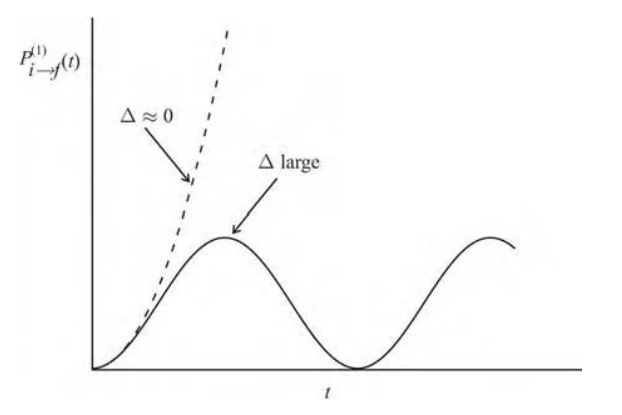
\includegraphics[scale=0.3]{p}
	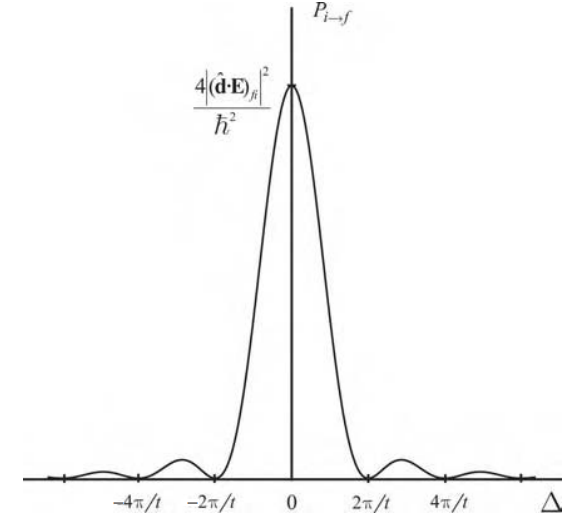
\includegraphics[scale=0.3]{t}
\end{figure}
For the perturbation approximation to be valid we require that $C^{(1)}_f(t) \ll 1$, which implies $P_{i \to f}^{(1)}(t) \ll 1$. For $\Delta \neq 0$, this places constraints on both $\abs{\lp \hat{\mathbf{d}}\cdot\mathbf{E}_0 \rp_{fi}}$ and $\Delta$. On resonance, \eqref{resonance} is only valid for a very short time. For the case of the transition probability as a function of $\Delta$, the width of the peak is proportional to $t^{-1}$ while the height is proportional to $t^2$. It turns out that the area is proportional to $t$:
\begin{align}
\int^{\infty}_{-\infty} \f{\sin^2 \Delta t/2}{\Delta^2} \,d\Delta = \f{\pi t}{2}
\end{align}
In the limit where $\Delta \approx 0$ and $t \gg 2\pi/\omega_{fi}$, the function in the integrand may be approximated by the Dirac delta function
\begin{align}
\lim_{t\to\infty}\f{\sin^2 \Delta t/2}{\Delta^2} = \f{\pi}{2}t\delta(\Delta).
\end{align}
In this case the transition probability is
\begin{align}
P^{(1)}_{i\to f}(t) = \f{\pi}{2}\abs{C^{(1)}_f(t)}^2 = \f{\abs{\lp \hat{\mathbf{d}}\cdot\mathbf{E}_0 \rp_{fi}}^2}{\hbar^2} t \delta(\Delta).
\end{align}
Now we define the time-independent transition probability \textbf{rate} as
\begin{align}
W_{i\to f} = \f{P^{(1)}_{i\to f}}{t} = \f{\pi}{2} \f{\abs{\lp \hat{\mathbf{d}}\cdot\mathbf{E}_0 \rp_{fi}}^2}{\hbar^2} \delta(\omega - \omega_{fi}).
\end{align}
In practice, the driving field will not be monochromatic so that a range of
frequencies will have to be summed or integrated over to obtain the total transition rate.  If $[f]$ represents a set of accessible final states, then the transition rate for a monochromatic field is
\begin{align}
\boxed{W_{i\to [f]} = \f{\pi}{2}\sum_{[f]}\f{\abs{\lp \hat{\mathbf{d}}\cdot\mathbf{E}_0 \rp_{fi}}^2}{\hbar^2} \delta(\omega - \omega_{fi})}
\end{align}
This expression is often famously called Fermi's Golden Rule. Now suppose there is a broad range of frequencies. This means the amplitude of the light is now frequency dependent $\mathbf{E}_0 \to \mathbf{E}_0(\omega)$. Thus the transition probability rate induced by all the frequency components must be
\begin{align}
\f{P^{(1)}_{i\to f}}{t} &=  \int \, d\omega \f{\abs{\lp \hat{\mathbf{d}}\cdot\mathbf{E}_0 \rp_{fi}}^2}{\hbar^2} \f{\sin^2(\Delta t/2)}{\Delta^2}\\
&= \f{1}{\hbar}\int \,d\omega \f{\sin^2(\Delta t/2)}{\Delta^2} \underbrace{\abs{\bra{f}\hat{\mathbf{d}\cdot\mathbf{E}_0(\omega)}\ket{i}}^2}_{F(\omega)}.
\end{align}
Now if $F(\omega)$ varies slowly with $\omega$ compared to $\f{\sin^2(\Delta t/2)}{\Delta^2}$ then we can take $F(\omega)$ to be its resonant value $F(\omega_{fi})$. With this we can take it out of the integral and get
\begin{align}
W_{i\to f} = \f{P^{(1)}_{i\to f}}{t} = \f{\pi}{2\hbar^2}F(\omega_{fi}).
\end{align}
The spread of the frequencies results in the dephasing of the oscillations as shown in the plot of transition probability versus time. This is due to the fact that the light in \textit{incoherent} (lacking the phase relations between the various frequency components). If the atom is driven by coherent light (like a laser), dephasing don't occur and the perturbative time-independent transition rates above generally do not adequately describe the dynamics. We will resolve this issue later. 






 
\subsection{Interaction of an atom with a quantized field \& Spontaneous emission}

In the previous subsection, we did not make any assumption about the relative position of the states $i$ and $f$, i.e., whether $E_i$ is greater or less than $E_f$. We simply said that so long as $\mathbf{E}_0 \neq 0$ and $E_i \neq E_f$, there is some non-zero transition probability. In this section, we will now show that for the case $E_i > E_f$, when the field is quantized, transitions will occur even when no photons are present. This is called \textit{spontaneous emission}. This is one of many differences that appear when we treat the field quantum mechanically versus classically. \\

Let us revisit the single-mode free space field given by \eqref{dipoleE} after dipole approximation (where we assumed the field is uniform over the atom):
\begin{align}
\hat{\mathbf{E}}(\mathbf{r},t)  \approx \hat{\mathbf{E}}(t) = i \lp \f{\hbar\omega_k}{2\epsilon_0 V} \rp^{\f{1}{2}}\mathbf{e} \lb \hat{a}e^{-i\omega t} - \hat{a}^\dagger e^{i\omega t} \rb.
\end{align}
But also recall that this free-space field is written in the Heisenberg picture (there is a time-dependence when the field operator is expressed in the Heisenberg basis). In the Schr\"{o}dinger picture, though, the field operator becomes
\begin{align}
\hat{\mathbf{E}} = i \lp \f{\hbar\omega_k}{2\epsilon_0 V} \rp^{\f{1}{2}}\mathbf{e} \lb \hat{a} - \hat{a}^\dagger \rb.
\end{align}

Now, the free-space Hamiltonian $\hat{\ham}_0$ must be
\begin{align}
\hat{\ham}_0 = \hat{\ham}_\text{atom} + \hat{\ham}_\text{field}
\end{align}
where $\hat{\ham}_\text{atom}$ is just the free-atom Hamiltonian as before and $\hat{\ham}_\text{field}$ is the free-space field Hamiltonian, which we have seen before as well:
\begin{align}
\hat{\ham}_\text{field} = \hbar\omega\lp \hat{a}^\dagger\hat{a} + \f{1}{2} \rp.
\end{align}
Now, because the zero-point energy term does not contribute to the dynamics, we will simply drop it. With this, the interaction Hamiltonian is given by
\begin{align}
\hat{\ham}^{(I)} = -\hat{\mathbf{d}} \cdot\hat{\mathbf{E}} = - i \lp \f{\hbar\omega_k}{2\epsilon_0 V} \rp^{\f{1}{2}}\lp \hat{\mathbf{d}}\cdot\mathbf{e} \rp \lp \hat{a} - \hat{a}^\dagger\rp.
\end{align}
Let us define
\begin{align}
\bm{\mathcal{E}}_0 = i \lp \f{\hbar\omega_k}{2\epsilon_0 V} \rp^{\f{1}{2}}\mathbf{e}.
\end{align}
From this,
\begin{align}
\hat{\ham}^{(I)} = - \hat{\mathbf{d}}\cdot\bm{\mathcal{E}}_0\lp \hat{a} - \hat{a}^\dagger\rp.
\end{align}

Now, because both the atomic and field systems are quantized, the states of the combined system is the product of the states of both the atom and field. Suppose initially we're given the initial state of the atom $\ket{a}$ and $n$ photons $\ket{n}$, then the initial state of the system is
\begin{align}
\ket{i} = \ket{a}\ket{n}. 
\end{align} 
The perturbation interaction of the quantized field causes a transition to the new state 
\begin{align}
\ket{f_1} = \ket{b}\ket{n-1}
\end{align}
where $n-1$ means that one photon has been absorbed by the atom to transition from $\ket{a}$ to $\ket{b}$, or to the state
\begin{align}
\ket{f_2} = \ket{b}\ket{n+1}
\end{align}
where $n+1$ means that one photon has been emitted by the atom to transition from $\ket{a}$ to $\ket{b}$. The energy of these states are
\begin{align}
&\text{for } \ket{i} = \ket{a}\ket{n}, \quad\quad\quad\, E_i = E_a + n\hbar\omega \\
&\text{for } \ket{f_1} = \ket{b}\ket{n-1}, \quad E_i = E_b + (n-1)\hbar\omega \\
&\text{for } \ket{f_2} = \ket{b}\ket{n+1}, \quad E_i = E_b + (n+1)\hbar\omega
\end{align}
where $E_a$ and $E_b$ are the energies of the atomic states $\ket{a}$ and $\ket{b}$. \\

We observe that the interaction Hamiltonian (or the Hamiltonian associated with the perturbation) is time-independent. The matrix elements of this interaction can be calculated by finding
\begin{align}
\text{Absorption: } &\bra{f_1}\hat{\ham}^{(I)}\ket{i}\\
\text{Emission: } &\bra{f_2}\hat{\ham}^{(I)}\ket{i}.
\end{align}
For absorption, we need a term in the interaction Hamiltonian that contains only the annihilation operator:
\begin{align}
\textbf{Absorption: } \bra{f_1}\hat{\ham}^{(I)}\ket{i}
&= \bra{b, n-1}-\hat{\mathbf{d}}\cdot\bm{\mathcal{E}}_0(\hat{a})\ket{a,n}\\
&= \bra{b,n-1}-\hat{\mathbf{d}}\cdot\bm{\mathcal{E}}_0 \sqrt{n}\ket{a,n-1}\\
&= \bra{b}-\hat{\mathbf{d}}\cdot\bm{\mathcal{E}}_0\ket{a}\sqrt{n}\braket{n-1}\\
&= \boxed{-\lp \hat{\mathbf{d}}\cdot\bm{\mathcal{E}}_0 \rp_{ba}\sqrt{n}}
\end{align}
Similarly, for emission
\begin{align}
\textbf{Emission: } \bra{f_2}\hat{\ham}^{(I)}\ket{i}
&= \bra{b, n+1}-\hat{\mathbf{d}}\cdot\bm{\mathcal{E}}_0(-\hat{a}^\dagger)\ket{a,n}\\
&= \bra{b,n+1}\hat{\mathbf{d}}\cdot\bm{\mathcal{E}}_0 \sqrt{n+1}\ket{a,n+1}\\
&= \bra{b}\hat{\mathbf{d}}\cdot\bm{\mathcal{E}}_0\ket{a}\sqrt{n+1}\braket{n+1}\\
&= \boxed{\lp \hat{\mathbf{d}}\cdot\bm{\mathcal{E}}_0 \rp_{ba}\sqrt{n+1}}
\end{align}
where
\begin{align}
\lp \hat{\mathbf{d}}\cdot\bm{\mathcal{E}}_0 \rp_{ba} = \bra{b}\hat{\mathbf{d}}\cdot\bm{\mathcal{E}}_0\ket{a} = \bra{b}\hat{\mathbf{d}}\ket{a}\cdot\bm{\mathcal{E}}_0 \equiv \mathbf{d}_{ba}\cdot\bm{\mathcal{E}}_0
\end{align}
is the dipole matrix element between states $\ket{b}$ and $\ket{a}$. \\

It is worthy to compare this result to the semiclassical picture we saw in the last subsection. For the absorption case, there is nothing new: if no field then no absorption: 
\begin{align}
n=0 \implies \bra{f_1}\hat{\ham}^{(I)}\ket{i} = 0
\end{align}
since $\sqrt{n} = 0$. However, the emission case has no semiclassical counterpart: transitions may occur even when no photons are present:
\begin{align}
n=0 \centernot\implies \bra{f_2}\hat{\ham}^{(I)}\ket{i} = 0
\end{align}
since $\sqrt{n+1}\neq 0$. This is called \textbf{spontaneous emission}, which cannot be obtained from the semiclassical approach. If $n > 0$, the emission of an additional photon is called \textbf{stimulated emission}, which is essential for the operation of the ``light amplification by stimulated emission of radiation'' or LASER. \\

We might also be interested in the ratio of the absorption/emission rates:
\begin{align}\label{rates}
\boxed{\f{\abs{\bra{f_2}\hat{\ham}^{(I)}\ket{i}}^2}{\abs{\bra{f_1}\hat{\ham}^{(I)}\ket{i}}^2}= \f{n+1}{n}}
\end{align}

It turns out that we can still use the perturbation method developed in the previous section to calculate the transition amplitudes, provided that me make appropriate modifications to account for the fact that the field is now quantized. The first difference is in the Hamiltonians:
\begin{align}
\hat{\ham}_0 = \hat{\ham}_\text{atom}  &\to \hat{\ham}_0 =  \hat{\ham}_\text{atom} + \hat{\ham}_\text{field}\\
\hat{\ham}^{(I)}(t) = -\hat{\mathbf{d}}\cdot\mathbf{E}(t) &\to \hat{\ham}^{(I)}(t) = - \hat{\mathbf{d}}\cdot\bm{\mathcal{E}}_0\lp \hat{a} - \hat{a}^\dagger\rp
\end{align}
where of course
\begin{align}
\hat{\ham}_\text{field} = \hbar\omega\lp \hat{a}^\dagger\hat{a} + \f{1}{2} \rp
\end{align}
where we again leave out the zero-point energy term. \\

Now, let us assume that the atom has only two levels $\ket{a}$ and $\ket{b}$. The state vector of the system can be written as
\begin{align}
\ket{\psi(t)} = &C_i(t)\ket{a}\ket{n}e^{-i\omega_a t}e^{-i n \omega t } \nonumber\\
&+ C_{f_1}(t)\ket{b}\ket{n-1}e^{-i\omega_b t}e^{-i (n-1) \omega t } \nonumber\\
&+ C_{f_2}(t)\ket{b}\ket{n+1}e^{-i\omega_b t}e^{-i (n+1) \omega t } 
\end{align}
where the first term is the initial state of the system, the second term is corresponds to absorption, and the third term corresponds to emission. We assume that $\ket{\psi(t)} = \ket{a}\ket{n}$, $C_i(0) = 1$, and $C_{f_1}(0) = C_{f_2}(0) = 0$. Following the perturbative method used before, we can get the first-order correction
for the amplitudes $C_{f_1}$ and $C_{f_2}$ associated with the atom being in state $\ket{b}$:
\begin{align}
\text{Absorption: }&C_{f_1}^{(1)}(t) = -\f{i}{\hbar}\int_0^t \,dt' \bra{f_1}\hat{\ham}^{(I)}\ket{i}e^{i(\omega_{f_1} - \omega_i)t'}\\
\text{Emission: }&C_{f_2}^{(1)}(t) = -\f{i}{\hbar}\int_0^t \,dt' \bra{f_2}\hat{\ham}^{(I)}\ket{i}e^{i(\omega_{f_2} - \omega_i)t'}.
\end{align}
And so the amplitude of the atom being in state $\ket{b}$ (to first-order of course) regardless of how it got there is the \textit{sum} of these amplitudes:
\begin{align}\label{quantum_amp}
C_f^{(1)}(t) &= C_{f_1}^{(1)}(t) + C_{f_2}^{(1)}(t)\\
&= \f{i}{\hbar}\lp \hat{\mathbf{d}}\cdot\bm{\mathcal{E}}_0 \rp_{ba}\int^t_0 \,dt'  \sqrt{n}  e^{i(\omega_{f_1} - \omega_i)t'} 
- \sqrt{n+1}  e^{i(\omega_{f_2} - \omega_i)t'}\\
&= \boxed{\f{i}{\hbar}\lp \hat{\mathbf{d}}\cdot\bm{\mathcal{E}}_0 \rp_{ba}
\lb \underbrace{\sqrt{n+1}\cdot\f{e^{i(\omega + \omega_{ba})t} - 1}{ \omega + \omega_{ba} }}_\text{Emission}  - \underbrace{\sqrt{n}\cdot\f{e^{i(\omega - \omega_{ba})t} - 1}{\omega - \omega_{ba}}}_{\text{Absorption}}\rb}
\end{align}
If $n\ll 1$ then $\sqrt{n+1} \approx \sqrt{n}$, in which case this result and \eqref{amplitude} are essentially the same and we get a correspondence between classical and quantum field amplitudes:
\begin{align}
\lp \mathbf{E}_0 \rp_\text{classical} \leftrightarrow \lp 2i\mathcal{E}_0\sqrt{n} \rp_\text{quantum}.
\end{align}

If $E_b > E_a$ ($\ket{b}$ is the excited state) and $\omega \approx \omega_{ba}$ then by RWA the first term in \eqref{quantum_amp} can be dropped as the second term dominates. There is nothing abnormal about this. However, if $E_a > E_b$ ($\ket{a}$ is the excited state) and $\omega \approx -\omega_{ba}$, then the second term of \eqref{quantum_amp} can be dropped (again under RWA). This leaves us with
\begin{align}
C_f^{(1)}(t) \approx \f{i}{\hbar}\lp \hat{\mathbf{d}}\cdot\bm{\mathcal{E}}_0 \rp_{ba}
\lb \underbrace{\sqrt{n+1}\cdot\f{e^{i(\omega + \omega_{ba})t} - 1}{ \omega + \omega_{ba} }}_\text{Emission}\rb.
\end{align}
We notice that even when $n=0$, this does not vanish. In this case, the transition between $\ket{a}$ and $\ket{b}$ occurs through spontaneous emission. 




\subsubsection{Field-theoretic derivation of the Planck's distribution}

Suppose we have a collection of atoms interacting resonantly with a quantized field of frequency
\begin{align}
\omega = \f{E_a - E_b}{\hbar}
\end{align}
where $\ket{a}$ and $\ket{b}$ are atomic eigenstates with $E_a > E_b$. Let $N_a, N_b$ be the populations of atoms in $\ket{a}$ and $\ket{b}$ respectively. Let $W_\text{emis}$ and $W_\text{abs}$ be the transition rate due to photon emission and absorption respectively. We have the following set of differential equations:
\begin{align}
&\f{dN_a}{dt} = -N_a W_\text{emis} + N_b W_\text{abs}\\
&\f{dN_b}{dt} = -N_b W_\text{abs} + N_a W_\text{emis}.
\end{align}
At thermal equilibrium:
\begin{align}
\f{dN_a}{dt} = 0 = \f{dN_b}{dt} \implies N_a W_\text{emis} = N_b W_\text{abs}.
\end{align}
From the relative rates in \eqref{rates}, we have
\begin{align}\label{1}
\f{N_b}{N_a} = \f{W_\text{emis}}{W_\text{abs}} = \f{n+1}{n}.
\end{align}
Now, according to Boltzmann statistics:
\begin{align}\label{2}
\f{N_b}{N_a} = e^{(E_a - E_b)/kT} = e^{\hbar\omega /kT}. 
\end{align}
From \eqref{1} and \eqref{2} we have
\begin{align}
\boxed{n = \f{1}{e^{\hbar\omega/kT} - 1}}
\end{align}

There's a slightly different derivation by Einstein (which was done even before quantum electrodynamics was invented), which takes into account as well the distinction between spontaneous and stimulated emission. We won't go into the details of this. 



\subsection{The Rabi model}

In the previous subsections we have used the perturbation theory approach to calculate transition probabilities. This approach assumes that the population in the initial state is essentially unchanged and the population in the final states are very small. This approach fails in cases of large population transfer, for example when there is a strong, near resonance (with one state and no other) laser field. In this case, the perturbation approach must be abandoned, only two dominant states remain, and the problem can solved ``exactly.'' This is the \textbf{Rabi model}. We note that the Rabi model is a \textit{semiclassical model}. The full quantum mechanical model is covered in the next subsection. \\

Suppose our two levels are the ground $\ket{g}$ and excited state $\ket{e}$. The transition frequency is given by
\begin{align}
\omega_0 = \f{E_e - E_g}{\hbar} \approx \omega
\end{align}
where $\omega$ is the frequency of the driving field. Once again, the interaction Hamiltonian is given by
\begin{align}
\hat{\ham}^{(I)} = -\hat{\mathbf{d}}\cdot\mathbf{E}_0 \cos\omega t \equiv \hat{V}_0 \cos\omega t
\end{align}
where again the dipole approximation is already made. The state vector is a linear combination of the eigenstates:
\begin{align}
\ket{\psi(t)} = C_g(t)e^{-iE_gt/\hbar}\ket{g} + C_e(t)e^{-iE_et/\hbar}\ket{e}.
\end{align}
The Schr\"{o}dinger equation
\begin{align}
i\hbar \f{\p \ket{\psi(t)}}{\p t} &= \lp \hat{\ham}_0 + \hat{\ham}^{(I)} \rp \ket{\psi(t)}\\
&=\lp \hat{\ham}_0 + \hat{V}_0 \cos\omega t \rp \ket{\psi(t)}
\end{align}
gives a system of differential equations:
\begin{align}
\begin{bmatrix}
\dot{C}_g \\ \dot{C}_e
\end{bmatrix}
=
\begin{bmatrix}
0 &-\f{i}{\hbar}\bra{g}\hat{V}_0 \ket{e}e^{-i\omega_0 t} \\ 
-\f{i}{\hbar}\bra{g}\hat{V}_0 \ket{e}e^{i\omega_0 t} & 0
\end{bmatrix}
\begin{bmatrix}
C_g \\ C_e
\end{bmatrix}
\end{align}
where the first equation is obtained by multiplying the SE from the left by $e^{i\omega_g t}\bra{g}$ and the fact that $\bra{i}\hat{V}_0\ket{j} = 0$ when $i = j$. Next, we assume that $\bra{g}\hat{V}_0 \ket{e}$ is real and $C_g(0) = 1, C_e(0) = 0$. Let us call
\begin{align}
\mathcal{V} = \bra{g}\hat{V}_0 \ket{e}
\end{align}
and approximate $\cos\omega t$ in exponentials and keep only the terms that oscillate at frequency $\omega - \omega_0$ to get
\begin{align}
&\dot{C}_g = -\f{i}{2\hbar}\mathcal{V}e^{i(\omega - \omega_0 )t}C_e\\
&\dot{C}_e = -\f{i}{2\hbar}\mathcal{V}e^{-i(\omega - \omega_0 )t}C_g.
\end{align}
Taking the derivative of the second equation, plugging it into the first while applying RWA (eliminating terms with $\omega + \omega_0$) we get
\begin{align}
\ddot{C}_e + i(\omega - \omega_0 )\dot{C}_e + \f{1}{4}\f{\mathcal{V}^2}{\hbar^2}C_e = 0.
\end{align}
This differential equation is quite a classic. The general solution is
\begin{align}
C_e(t) = A_+ e^{i\lambda_+ t} + A_- e^{i\lambda_- t} 
\end{align}
where with $\Delta = \omega - \omega_0$,
\begin{align}
\lambda_{\pm} = \f{1}{2}\lb \Delta \pm \sqrt{ \Delta^2 + \f{\mathcal{V}^2}{\hbar^2}} \rb.
\end{align}
From the initial conditions, we also have that
\begin{align}
A_{\pm} = \mp \f{1}{2\hbar}\f{\mathcal{V}}{\sqrt{\Delta^2 + \f{\mathcal{V}^2}{\hbar^2}}}.
\end{align}
With this, the solution to the problem is
\begin{align}
&C_e(t) = i\f{\mathcal{V}}{\Omega_R \hbar}e^{i\Delta t/2}\sin\f{\Omega_R t}{2}\\
&C_g(t) = e^{i\Delta t/2} \lc \cos\f{\Omega_R t}{2} - i\f{\Delta}{\Omega_R}\sin\f{\Omega_R t}{2} \rc
\end{align}
where
\begin{align}
\Omega_R = \sqrt{\Delta^2 + \f{\mathcal{V}^2}{\hbar^2}}
\end{align}
is called the \textbf{Rabi frequency}, or \textbf{Rabi rate}. \\

The probability that the atom is in the excited state $\ket{e}$ is then
\begin{align}
\boxed{P_e(t) = \abs{C_e(t)}^2 = \f{\mathcal{V}^2}{\Omega_R^2\hbar^2}\sin^2\f{\Omega_R t}{2}}
\end{align}
On resonance, this probability is a perfect sine-squared:
\begin{align}
\boxed{P_e(t) = \sin^2\f{\mathcal{V}t}{2\hbar}}
\end{align}
where at $t= \pi \hbar / \mathcal{V}$ all the atomic population is transferred to the excited state. The following plot illustrates the population transfer and ``oscillation''
\begin{figure}[!htb]
	\centering
	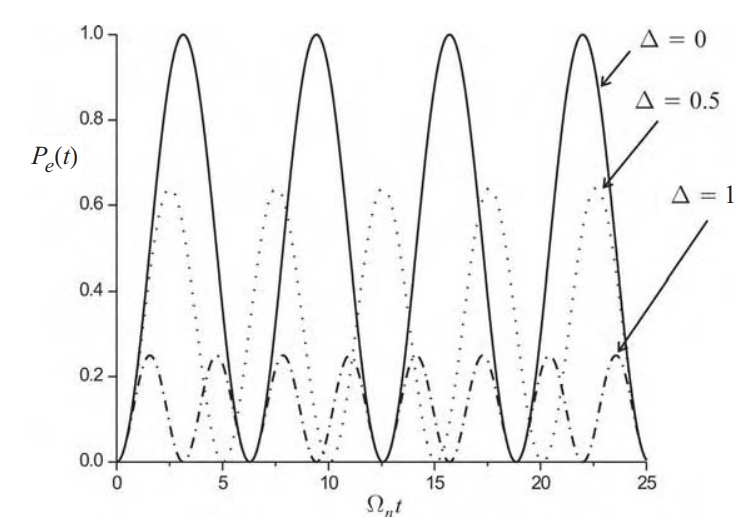
\includegraphics[scale=0.3]{rabi}
\end{figure}

The \textbf{atomic inversion} $W(t)$ is defined as the difference in population between the excited and ground states:
\begin{align}
W(t) = P_e(t) - P_g(t).
\end{align}
For the case of resonance ($\Delta = 0$) and that initially the atom is in the ground state, 
\begin{align}
W(t) = \sin^2 \f{\mathcal{V}t}{2\hbar} - \cos^2 \f{\mathcal{V}t}{2\hbar} = -\cos\f{\mathcal{V}t}{\hbar} = -\cos\Omega_R(\Delta = 0)t.
\end{align}
For $t = \pi\hbar/\mathcal{V}$, $W(\pi\hbar/\mathcal{V}) = 1$. This kind of population transfer is called the $\pi-$pulse. For $t = \pi\hbar/2\mathcal{V}$, $W(\pi\hbar/2\mathcal{V}) = 0$, which means the population is shared coherently between the ground and excited states, i.e., the system is in a perfect superposition:
\begin{align}
\ket{\psi(t)} = \f{1}{\sqrt{2}}\lp\ket{g} + i\ket{e} \rp.
\end{align}










\subsection{Fully quantum-mechanical model; the Jaynes–Cummings model}

We move on to the quantum electrodynamics version of the Rabi model. In our previous discussion of the interaction between atoms and the quantized field, we assumed the field is single-mode. We again assume this, such that the single-mode cavity field can be written as
\begin{align}
\mathbf{\hat{E}} = \mathbf{e}\lp \f{\hbar\omega}{\epsilon_0 V} \rp^{1/2}\lp \hat{a} + \hat{a}^\dagger\rp\sin(kz)
\end{align}
where $\mathbf{e}$ is some arbitrary polarization vector. We also assume that the atom has two levels $\ket{g}$ and $\ket{e}$. The interaction Hamiltonian is given by
\begin{align}
\hat{\ham}^{(I)} = -\mathbf{\hat{d}} \cdot \mathbf{\hat{E}} = \hat{d} g (\hat{a} + \hat{a}^\dagger)
\end{align}
where
\begin{align}
\hat{d} &= \mathbf{d} \cdot \mathbf{e}\\
g &=  \lp \f{\hbar\omega}{\epsilon_0 V} \rp^{1/2}\sin(kz).
\end{align}

For simplicity, let us introduce the atomic transition operators 
\begin{align}
\text{Excitation: } &\hat{\sigma}_+ = \ket{e}\bra{g}\\
\text{De-excitation: } &\hat{\sigma}_- = \ket{g}\bra{e} = \hat{\sigma}_+^\dagger.
\end{align}
The inversion operator is given by
\begin{align}
\hat{\sigma}_3 = \ket{e}\bra{e} - \ket{g}\bra{g}.
\end{align}
We can verify that these operators obey the Pauli spin algebra:
\begin{align}
[\hat{\sigma}_+, \hat{\sigma}_-] &= \hat{\sigma}_3\\
[\hat{\sigma}_3, \hat{\sigma}_\pm] &= 2\hat{\sigma}_\pm.
\end{align}

We know that the diagonal matrix elements of $\hat{d}$ is zero because $\bra{e}\hat{d}\ket{e} = \bra{g}\hat{d}\ket{g} = 0$. This means with $d = \bra{e}\hat{d}\ket{g}$, we can write in the basis
\begin{align}
\hat{d} &= d\ket{g}\bra{e} + d^*\ket{e}\bra{g}\\
&= d\hat{\sigma}_- + d^*\hat{\sigma}_+\\
&= d\lp \hat{\sigma}_- + \hat{\sigma}_+ \rp.
\end{align}
This gives the interaction Hamiltonian:
\begin{align}
\hat{\ham}^{(I)} = \hbar \lp \f{dg}{\hbar} \rp \lp \hat{\sigma}_- + \hat{\sigma}_+ \rp \lp \hat{a} + \hat{a}^\dagger \rp. 
\end{align}
Define the energy to be zero halfway between the states, then we have $E_e = -E_g$, and the free atomic Hamiltonian can be written as
\begin{align}
\hat{\ham}_0 = \f{\hbar}{2}\begin{bmatrix}
E_e & \\ & E_g
\end{bmatrix} 
\end{align}
or in the basis
\begin{align}
\hat{\ham}_0 = \f{1}{2}\hbar\omega_0 \lp \ket{e}\bra{e} - \ket{g}\bra{g} \rp = \f{1}{2}\hbar\omega_0 \hat{\sigma}_3 
\end{align}
where 
\begin{align}
E_e = -E_g = \f{1}{2}\hbar\omega_0
\end{align}
and of course $\omega_0$ is the transition frequency. The free-field Hamiltonian after dropping the zero-point energy term, again, is
\begin{align}
\hat{\ham}_F = \hbar\omega\hat{a}^\dagger\hat{a}.
\end{align}
So the total Hamiltonian is
\begin{align}
\hat{\ham} &= \hat{\ham}_0 + \hat{\ham}_F + \hat{\ham}^{(I)}\\
&= \f{1}{2}\hbar\omega_0 \hat{\sigma}_3  + \hbar\omega\hat{a}^\dagger\hat{a} + \hbar \lp \f{dg}{\hbar} \rp \lp \hat{\sigma}_- + \hat{\sigma}_+ \rp \lp \hat{a} + \hat{a}^\dagger \rp.
\end{align}
Let us call
\begin{align}
\lambda = \f{dg}{h}.
\end{align}
It follows that
\begin{align}
\hat{\ham} = \f{1}{2}\hbar\omega_0 \hat{\sigma}_3  + \hbar\omega\hat{a}^\dagger\hat{a} + \hbar \lambda\lp  \hat{\sigma}_- + \hat{\sigma}_+ \rp \lp \hat{a} + \hat{a}^\dagger \rp.
\end{align}
Let us simplify this Hamiltonian with some approximations. We know that in the field-free case, the creation and annihilation operators evolve in time as
\begin{align}
\hat{a}(t) = \hat{a}(0)e^{-i\omega t} \hspace{0.5cm} \hat{a}^\dagger(t) = \hat{a}^\dagger(0)e^{i\omega t},
\end{align}
while in the free atomic case the excitation operators (which we can show) to evolve in time as
\begin{align}
\hat{\sigma}_{\pm}(t) = \hat{\sigma}_\pm(0)e^{\pm i \omega_0 t}.
\end{align}
This gives us some idea of the time dependency of the product of some of these operators:
\begin{align}
&\hat{\sigma}_+ \hat{a} \sim e^{i(\omega_0 - \omega)t}\\
&\hat{\sigma}_- \hat{a}^\dagger \sim e^{-i(\omega_0 - \omega)t}\\
&\hat{\sigma}_+ \hat{a}^\dagger \sim e^{i(\omega_0 + \omega)t}\\
&\hat{\sigma}_- \hat{a} \sim e^{-i(\omega_0 + \omega)t}.
\end{align}
For $\omega_0 \approx \omega$ we can use RWA to ignore the last two terms. The term $\hat{\sigma}_+ \hat{a}^\dagger$ corresponds to the emission of a photon (the creation operator) as the atom goes from the ground to the excited state, while the term $\hat{\sigma}_- \hat{a}$ corresponds to the absorption of a photon (the annihilation operator) as the atom goes from the excited to ground state. It makes good sense to ignore these terms, so that we're left with the approximate Hamiltonian:
\begin{align}
\boxed{\hat{\ham} = \f{1}{2}\hbar\omega_0 \hat{\sigma}_3  + \hbar\omega\hat{a}^\dagger\hat{a} + \hbar \lambda\lp  \hat{\sigma}_+ \hat{a}  + \hat{\sigma}_-\hat{a}^\dagger \rp}
\end{align}
This is called the \textbf{Jaynes-Cummings model}. To solve the dynamics of the system, we first note a few constants. The first constants is the number of electrons, or the total probability of the atom being in either state $\ket{e}$ or $\ket{g}$:
\begin{align}
\hat{P}_E = \ket{e}\bra{e} + \ket{g}\bra{g} = 1.
\end{align}
and of course this quantity is conserved: 
\begin{align}
[\hat{\ham}, \hat{P}_E] \propto \f{d\hat{P}_E}{d t} = 0.
\end{align}
The excitation number is also unchanged: 
\begin{align}
\hat{N}_e = \hat{a}^\dagger\hat{a} + \ket{e}\bra{e} \implies [\hat{\ham}, \hat{N}_e] \propto \f{d\hat{N}_e}{dt} = 0.
\end{align}
This equation essentially says the number of electrons created corresponds to the transitions.\\

With these constants we may break the Hamiltonian into two commuting parts:
\begin{align}
\hat{\ham} = \hat{\ham}_I + \hat{\ham}_{II}
\end{align}
where
\begin{align}
\hat{\ham}_I &= \hbar\omega \hat{N}_e + \hbar\lp \f{\omega_0}{2} - \omega \rp\hat{P}_E\\
\hat{\ham}_{II} &= -\hbar\Delta + \hbar \lambda \lp \hat{\sigma}_+ \hat{a}  + \hat{\sigma}_-\hat{a}^\dagger \rp
\end{align}
All dynamics is contained in $\hat{H}_{II}$, while $\hat{\ham}_I$ contributes to (irrelevant) phase factors. Next, let us examine a few notable cases. 

\subsubsection{Resonance: $\Delta = 0$}

Let us assume that initially the atom is in the excited state $\ket{e}$ and the field is initially in the state $\ket{n}$. The initial atom-field state is
\begin{align}
\ket{i} = \ket{e}\ket{n}.
\end{align}
The energy of this state is of course
\begin{align}
E_i  = E_e + E_n = \f{1}{2}\hbar\omega + n\hbar\omega
\end{align}
where recall that we have set zero energy to be in the middle of the two states. This initial state $\ket{i}$ to coupled to and only to the final state $\ket{f} = \ket{g}\ket{n+1}$. The state vector is given by
\begin{align}
\ket{\psi(t)} = C_i(t) \ket{i} + C_f(t)\ket{f}
\end{align}
with $C_i(0) = 1$ and $C_f(0) = 0$. In the interaction picture, 
\begin{align}
i\hbar \f{d\ket{\psi(t)}}{dt} = \hat{\ham}_{II}\ket{\psi(t)}.
\end{align}
Plugging $\hat{\ham}_{II}$ in and solve we obtain
\begin{align}
\dot{C}_i &= -i\lambda \sqrt{n+1}C_f\\
\dot{C}_f &= -i\lambda \sqrt{n+1}C_i. 
\end{align}
By eliminating $C_f$ and solving, we get 
\begin{align}
C_i(t) = \cos\lp  \lambda t \sqrt{n+1} \rp
\end{align}
and 
\begin{align}
C_f(t) =-i\sin\lp \lambda t \sqrt{n+1} \rp.
\end{align}
With this, the probability that the system is in the initial state is
\begin{align}
P_i(t) = C_i^*(t)C_i(t) = \cos^2 \lp  \lambda t \sqrt{n+1} \rp.
\end{align}
And the probability that the system is in the other state is of course
\begin{align}
P_f(t) = \sin^2\lp  \lambda t \sqrt{n+1} \rp.
\end{align}
The atom inversion is then
\begin{align}
W(t) = P_i(t) - P_f(t) = \cos\lp 2\lambda t \sqrt{n+1} \rp.
\end{align}
We may define a quantum electrodynamic Rabi frequency
\begin{align}
\boxed{\Omega(n) = 2\lambda\sqrt{n+1}}
\end{align}
This gives
\begin{align}
W(t) = \cos\lp \Omega(n)t \rp.
\end{align}
We notice that there's Rabi oscillation, which we also see in the classical case. However, there is still Rabi oscillation in the case of $n=0$. These is vacuum Rabi oscillation. They are the result of the atom spontaneously emitting a photon then re-absorbing it, re-emitting it, etc.: an example of reversible spontaneous emission.


\subsubsection{Pure state}
In this scenario we assume that the atom is initially in a superposition of $\ket{e}$ and $\ket{g}$. 
\begin{align}
\ket{\psi(t)}_\text{atom} =C_e\ket{e} + C_g\ket{g}.
\end{align}
The field is initially in the state
\begin{align}
\ket{\psi(t)}_\text{field} = \sum_{n=0}^\infty C_n\ket{n}.
\end{align}
Thus the initial state of the system is given by a tensor product
\begin{align}
\ket{\psi(t)} = \ket{\psi(0)}_\text{atom} \otimes \ket{\psi(0)}_\text{field}.
\end{align}
The solution to the Schr\"{o}dinger equation is now
\begin{align}
\ket{\psi(t)} = \sum^\infty_{n=0}\lc \lb C_e C_n \cos (\lambda t \sqrt{n+1}) - iC_gC_{n+1}\sin(\lambda t \sqrt{n+1}) \rb \ket{e} \right. \nonumber \\  \left.
+ \lb -iC_eC_{n-1}\sin(\lambda t \sqrt{n}) + C_gC_n \cos(\lambda t \sqrt{n}) \rb 
 \rc \otimes \ket{n}.
\end{align}
This is an entangled state. Now, if $C_e = 1$ and $C_g = 0$ initially, then
\begin{align}
\ket{\psi(t)} = \ket{\psi_g(t)}\otimes \ket{g} + \ket{\psi_e(t)}\otimes \ket{e},
\end{align}
where
\begin{align}
&\ket{\psi_g(t)} = -i\sum^\infty_{n=0}C_n\sin(\lambda t \sqrt{n+1})\ket{n+1}\\
&\ket{\psi_e(t)} = \sum^\infty_{n=0}C_n\cos(\lambda t \sqrt{n+1})\ket{n}.
\end{align}
The atomic inversion is then
\begin{align}
W(t) &= \bra{\psi(t)}\hat{\sigma}_3\ket{\psi(t)}\\
&= \braket{\psi_e(t)} - \braket{\psi_g(t)}\\
&= \sum^\infty_{n=0}\abs{C_n}^2 \cos(2\lambda t\sqrt{n+1}).
\end{align}


\subsection{The Density Operator approach (or the master equation's approach) }
So far, we have considered only cases where the field and the atom are initially in pure states. The density operator approach allows us to solve for a more general case. Let us work in the interaction picture again where the interaction Hamiltonian is given by
\begin{align}
\hat{\ham}_I = \hbar\lambda \lp \hat{a}\hat{\sigma}_+ + \hat{a}^\dagger\hat{\sigma}_- \rp
\end{align}
Let us consider the density operator of the atom-field system at time $t$. As we know the density operator is defined to be
\begin{align}
\hat{\rho} = \ket{\psi}\bra{\psi}.
\end{align}
Applying the Schr\"{o}dinger equation to $\ket{\psi}$, we have
\begin{align}
i\hbar \f{d\ket{\psi}}{dt} = \hat{\ham}_I \ket{\psi}.
\end{align}
Now let us see what we get when we look at the time evolution of the density operator
\begin{align}
\f{d \hat{\rho}}{dt} &= \f{d\ket{\psi}}{dt} \bra{\psi} + \ket{\psi}\f{d\bra{\psi}}{dt}\\
&= \lb \f{-i}{\hbar}\hat{\ham}_I\ket{\psi} \rb\bra{\psi} + \ket{\psi}\lb \f{i}{\hbar}\bra{\psi} \hat{\ham}_I \rb\\
&= \f{-i}{\hbar}\lb \hat{\ham}_I\ket{\psi}\bra{\psi} - \ket{\psi}\bra{\psi}\hat{\ham}_I \rb\\
&= \f{-i}{\hbar}\lb \hat{\ham}_I, \hat{\rho} \rb.
\end{align}
The solution to this (which we can quite easily verify) is 
\begin{align}\label{rho}
\hat{\rho}(t) = e^{-i\hat{\ham}_I t/\hbar}\hat{\rho}(0)e^{i\hat{\ham}_I t/\hbar} = \hat{U}_I(t)\hat{\rho}(0)\hat{U}_I^\dagger(t).
\end{align} 
Recall that the Hamiltonian can be expressed further in terms of the excitation/de-excitation, and inversion operators, whose matrix representations are
\begin{align}
\sigma_+ = \begin{bmatrix}
0 & 1\\0 & 0
\end{bmatrix}, \hspace{0.5cm}
\sigma_- = \begin{bmatrix}
0 & 0 \\ 1 & 0
\end{bmatrix}, \hspace{0.5cm}
\sigma_3 = \begin{bmatrix}
1 & 0 \\ 0 & -1
\end{bmatrix}
\end{align}
where we have used the convention
\begin{align}
\sigma_j = \begin{bmatrix}
\bra{e}\hat{\sigma}_j\ket{e} & \bra{e}\hat{\sigma}_j\ket{g}\\
\bra{g}\hat{\sigma}_j\ket{e} &
\bra{g}\hat{\sigma}_j\ket{g} 
\end{bmatrix}, \hspace{0.5cm} j = \pm, 3.
\end{align}
Let us re-write $\hat{U}_I(t)$ in terms of these operators:
\begin{align}
\hat{U}_I(t) = e^{-i\hat{H}_I t/\hbar} = e^{-i\lambda t (\hat{a}\hat{\sigma}_+ + \hat{a}^\dagger\hat{\sigma_-})}.
\end{align}
With this, we can write the evolution operator $\hat{U}_I$ in terms of cosines and sines as
\begin{align}
\hat{U}_I(t) = \begin{bmatrix}
\hat{C}(t) & \hat{S}'(t) \\ \hat{S}(t) & \hat{C}'(t)
\end{bmatrix}
\end{align}
where
\begin{align}
&\hat{C}(t) = \cos(\lambda t \sqrt{\hat{a}\hat{a}^\dagger})\\
&\hat{S}(t) = -i\hat{a}^\dagger\f{\sin(\lambda t \sqrt{\hat{a}\hat{a}^\dagger})}{\sqrt{\hat{a}\hat{a}^\dagger}}\\
&\hat{C}'(t) = \cos(\lambda t \sqrt{\hat{a}^\dagger\hat{a}})\\
&\hat{S}'(t) =  -i\hat{a}\f{\sin(\lambda t \sqrt{\hat{a}^\dagger\hat{a}})}{\sqrt{\hat{a}^\dagger\hat{a}}}.
\end{align}
It is then easy to show that
\begin{align}
\hat{U}^\dagger_I(t) = \hat{U}_I(-t) = \begin{bmatrix}
\hat{C}(t) & -\hat{S}'(t) \\ -\hat{S}(t) & \hat{C}'(t)
\end{bmatrix}.
\end{align}
Now, suppose at $t=0$ the density operator for the atom-field system can be written as a tensor product of the field and atom parts (not entangled):
\begin{align}
\hat{\rho}(0) = \hat{\rho}^F(0)\otimes \hat{\rho}^A(0).
\end{align}
Next, suppose that our atom is initially in $\ket{e}$, such that by convention the atom's density matrix is
\begin{align}
\rho^A(0) = \begin{bmatrix}
1 & 0 \\ 0 & 0
\end{bmatrix}.
\end{align}
Thus for the system,
\begin{align}
\hat{\rho}(0) = \hat{\rho}^F(0) \otimes \begin{bmatrix}
1 & 0 \\ 0 & 0
\end{bmatrix} = \begin{bmatrix}
\hat{\rho}^F(0) & 0 \\ 0 & 0 
\end{bmatrix}.
\end{align}
Now by \eqref{rho},
\begin{align}
\hat{\rho}(t) = \begin{bmatrix}
\hat{C}(t)\hat{\rho}^F(0)\hat{C}(t) & -\hat{C}(t)\hat{\rho}^F(0)\hat{S}'(t)\\
\hat{S}(t)\hat{\rho}^F(0)\hat{C}(t) & -\hat{S}(t)\hat{\rho}^F(0)\hat{S}'(t)
\end{bmatrix}.
\end{align}

To find the density operator of the field, we trace over the atomic states:
\begin{align}
\hat{\rho}^F(t) = \Tr_A \hat{\rho}(t) = \hat{C}(t)\hat{\rho}^F(0)\hat{C}(t) -\hat{S}(t)\hat{\rho}^F(0)\hat{S}'(t).
\end{align}
The matrix elements for the field are then
\begin{align}
\hat{\rho}^F_{nm} &\equiv \bra{n}\hat{\rho}^F(t)\ket{m} \\ 
&= \bra{n} \hat{C}(t)\hat{\rho}^F(0)\hat{C}(t) \ket{m} - \bra{n} \hat{S}(t)\hat{\rho}^F(0)\hat{S}'(t) \ket{m}.
\end{align}
On the other hand, tracing over the field states (there are infinitely many) we obtain the density operator of the atom:
\begin{align}
\hat{\rho}^A(t) = \Tr_F \hat{\rho}(t) = \sum^\infty_{n=0} \bra{n}\hat{\rho}(t)\ket{n}.
\end{align}
The matrix elements are then
\begin{align}
\bra{i}\hat{\rho}^A(t)\ket{j} = \sum^\infty_{n=0}\bra{i,n} \hat{\rho}_F(t)\ket{j,n}
\end{align}
where $i,j = e,g$. The diagonal elements $\rho^A_{ee}$ and $\rho^A_{gg}$ are the populations of the excited and ground states and satisfy
\begin{align}
\rho^A_{gg}(t) + \rho^A_{ee}(t) = 1
\end{align}
for any time $t$. The atomic inversion is
\begin{align}
W(t) = \rho^A_{ee}(t) - \rho^A_{gg}(t) = 2\rho^A_{ee}(t) - 1.
\end{align}
We can find that
\begin{align}
\rho^A_{ee}(t) &= \sum^\infty_{n=0}\bra{n}\hat{C}(t)\hat{\rho}^F(0)\hat{C}(t)\ket{n}\\
&= \sum^\infty_{n=0}\bra{n}\hat{\rho}^F(0)\ket{n}\cos^2(\lambda t \sqrt{n+1}).
\end{align}
\subsubsection{Pure state}
If the field is initially in a pure state
\begin{align}
\ket{\psi_F(0)} = \sum^\infty_{n=0}C_n\ket{n},
\end{align}
then
\begin{align}
\hat{\rho}^F(0) = \ket{\psi_F}\bra{\psi_F},
\end{align}
which gives
\begin{align}
\rho^A_{ee}(t) = \sum^\infty_{n=0}\abs{C_n}^2\cos^2(\lambda t \sqrt{n+1}).
\end{align}
This gives the atomic inversion we have found before. 
\subsubsection{Mixed state}
However, if the field is initially in a thermal state (mixed state) where
\begin{align}
\hat{\rho}^F(0) = \hat{\rho}_{Th} = \sum P_n\ket{n}\bra{n}
\end{align}
where $P_n$ is probability. The atomic inversion in this case is
\begin{align}
W(t) = \sum^\infty_{n=0}P_n \cos(2\lambda t\sqrt{n+1}),
\end{align}
which is slightly different. 



















\newpage

\section{Collective Atomic Interactions}



\newpage


\chapter{QUANTUM INFORMATION}















\chapter{PROBLEMS \& SOLUTIONS}

\newpage

\section{Quantum Mechanics}

\newpage

\section{Quantum Optics}

\newpage

\section{Quantum Information}



\newpage

% move this somewhere else later

%One photon, two photons, red photon, blue photon.\\
%JQI Summer School\\
%Elizabeth Goldschmidt\\
%July 19, 2019\\
%
%Topic: single photon, single photon statistics. \\
%
%\textbf{Why?}
%\begin{itemize}
%	\item Why single photons?
%	\item Why is it hard?
%\end{itemize}
%
%
%\textbf{Sending QI}
%\begin{itemize}
%	\item Sending quantum information as light (not as easy any other way)
%	\item requires encoding qubits in light
%	\item qubits must be identical in all other degrees of freedom: polarizations, transverse/longitudinal modes....
%	\item How else can you do it LOL?
%\end{itemize}
%
%
%\textbf{Single photon: } single excitation of a single mode of the quantized EM field. This treats photon number differently from other dfs. There's a fundametal difference between 0 and multiple excitations. 
%
%\textbf{Photon number:}
%\begin{itemize}
%	\item Classical light: spectral and photon number distribution depend on system (source). 
%	\item Why can't I turn down intensity to get single photon? Because probability of getting 2 saturates.
%	\item Photon number is not a good quantum number.
%	\item So what do we do? $\implies$ reduce variance.
%	\item How to quantify? Use $g^{(2)}$ - autocorrelation function. For weak fields
%	\begin{align}
%	g^{(2)} = \f{conincidence}{individual\times individual} \approx = \f{2 p(2)}{p(1)^2}
%	\end{align}
%	independent of attenuation.
%	\item \textbf{Cauchy-Schwarz}. Classically, operators commute... 
%	such that $g^{(2)} \geq 1$ (no anti-bunching light). But because of QM, $g^{(2)}$ can be less than 1. 
%\end{itemize}
%
%
%\textbf{Other dfs: } the well-defined single mode covers all the other degrees of freedom (spatial, spectral, temporal, polarization, etc.) How to quantify single-photon? $\implies$ Two-photon (Hong-Ou-Mandel) Interference. 
%\begin{itemize}
%	\item Measure indistinguishability to characterize single photons. 
%\end{itemize}
%
%
%\textbf{Some single-photon technologies:} How do we make single-photons? 
%\begin{itemize}
%	\item \textit{Weak laser}: but there's no multi-photon suppression ($g^{(2)} = 1$) and low efficiency.
%	\item \textit{Single emitters}: Excite a two level system and collect spontaneous emission. However, emits to $4\pi$ (solid angle, everywhere), so difficult to collect. Also, if the excitation light is the same as the emission, then need strong filter. 
%	\item Trapped ions...
%	\item Two-mode squeezing/pair source (spontaneous parametric down conversion is an example), or ``perfect beam splitter''
%	\item Pair sources: single-arm statistics is classical. Often high spectrally multi-mode (different colors, and with different colors comes different indices of reflection, hence photons come out at different angles to conserve momentum)
%	\item Now if this is done in atomic ensemble instead of a non-linear crystal. This needs single-photon source on-demand. 
%\end{itemize}
%
%
%\textbf{Experiments at JQI:} 
%\begin{itemize}
%	\item Interfering photons from different single photon sources (detect with high time resolution)
%	\item Frequency resolved detection (detect with high frequency resolution)
%\end{itemize}
%
%
%
%
%
%
%
%
%\newpage
%
%
%\textbf{Kanu's talk, July 22, 2019.}\\
%
%\textbf{Superradiance:} Example: two dipoles radiating in phaes. Collective enahnced emission is superradiance. The amplitude adds, so intensity grows as n-squared. This is a classical effect.\\
%
%Now, what if there is time-delayed feedback? There is retardation and back action. SUPER-DUPER-RADIANCE. How far should the separation be? Distance should be comparable to coherence time. 
%\begin{align}
%\f{c}{2\gamma_0} < d < \f{c}{\gamma_0}
%\end{align}
%where $c/2\gamma_0$ is super-radiant photon coherent length versus independent (without factor of 2). This gives a paradox. Assume superradiant emission than don't get superradiance and vice versa. This means Markov approximation fails. 
%
%\begin{itemize}
%	\item Superradiance
%	\item Time-delayed feedback
%\end{itemize}
%
%Combining these gives super-duper-radiance. Here's the derivation. Assume two two-level system Hamiltonians, coupled to a waveguide $\ham_F$. Separation between the atoms is $d$. 
%\begin{align}
%\ham = \ham_{atom} + \ham_F + \ham_{int}
%\end{align}
%where
%\begin{align}
%\ham_{atom} =  \hbar\omega_0 \sum_{n=1,2}\hat{\sigma}_n^+ \hat{\sigma}_n^-
%\end{align}
%and
%\begin{align}
%\ham_F = \int \, d\omega \hbar\omega \hat{a}^\dagger_\omega \hat{a}_\omega.
%\end{align}
%The interaction is electric-dipole:
%\begin{align}
%\ham_{int} = \sum_{n=1,2} -\hat{d}_n \cdot \hat{E} \approx_{RWA} \int\,d\omega \hbar g(\omega) \sum_{n=1,2} \lb \hat{\sigma}_n^+ \hat{a}_\omega e^{i\vec{k}\cdot\vec{r}}  + h.c. \rb
%\end{align}
%where $k = \omega / v_g \hat{x}$ and $v_g$ is the velocity in the waveguide. Moving to the rotating frame, calling $\ham_0 = \ham_{atom} + \ham_{F}$. Call
%\begin{align}
%\tilde{\ham}_{int} = \U \ham_{int} \U^\dagger
%\end{align}
%where 
%\begin{align}
%\U = e^{-i\ham_0 t}.
%\end{align}
%With these,
%\begin{align}
%\tilde{\ham}_{int} = \int \, d\omega \hbar g(\omega)\sum_{n=1,2} \hat{\sigma}^+_n \hat{a}_\omega e^{- i (\omega - \omega_0) t}  e^{i \vec{k}\cdot\vec{r}} + h.c.
%\end{align}
%Suppose at $t=0$:
%\begin{align}
%\ket{\psi(0)} = \lp \ket{eg} + \ket{ge} \rp \otimes \ket{\{0\}}_F.
%\end{align}
%In general, under the Hamiltonian, restricting to single-excitation subspace
%\begin{align}
%\ket{\psi(t)} = C_1(t)\ket{eg} + C_2(t)\ket{ge} + \int \, d\omega C_\omega(t)\ket{gg}\otimes\ket{\{1_\omega\} }_F.
%\end{align}
%We want to study the dynamics of the coefficients. We define the positions of the atoms as $r_1 = d/2$, $r_2 = -d/2$.
%\begin{align}
%&\dot{C}_1(t) = -i\int\,d\omega g(\omega) C_\omega e^{-i(\omega - \omega_0)t} e^{-ikd/2}\\
%&\dot{C}_2(t) = -i\int\,d\omega g(\omega) C_\omega e^{-i(\omega - \omega_0)t} e^{ikd/2}.
%\end{align}
%The field dynamics:
%\begin{align}
%\dot{C}_\omega = -i g(\omega)\lb C_1 e^{-ikd/2} + C_2 e^{ikd/2} \rb e^{-i(\omega - \omega_0) t}.
%\end{align}
%So
%\begin{align}
%C_\omega(t) = -i \int^t_0 \,d \tau  g(\omega)\lb C_1 (\tau) e^{-ikd/2} + C_2 (\tau) e^{ikd/2} \rb e^{-i(\omega - \omega_0) \tau}.
%\end{align}
%Approximate: $g(\omega) \approx g(\omega_0) = g_0$ (flat spectral density). So
%\begin{align}
%\dot{C}_1(t) &= -g_0^2 \int_\infty \,d\omega e^{-i(\omega - \omega_0) t} e^{ikd/2}\int^t_0 \, d \tau \lb C_1 e^{-ikd/2} + C_2 e^{ikd/2} \rb e^{-i(\omega - \omega_0) \tau}\\
%&= -g_0^2 \int^t_0 \,d\tau \int_\infty \,d\omega \lc C_1(\tau) + C_2(\tau)e^{i\omega d/v_g} \rc e^{-i(\omega - \omega_0)(t-\tau)}\\
%&= -2\pi g_0^2 \int^t_0 \,d\tau C_1(\tau)\delta(t-t\tau) + C_2(\tau)\delta\lp t - \f{d}{v_g} - \tau \rp e^{i \omega_0 d/v_g}.
%\end{align}
%Now, approximate: $d\omega_0 /v_g = 1$. Call $-2\pi g_0^2 = -\gamma/2$ to get
%\begin{align}
%\dot{C}_1(t) &= -\f{\gamma}{2}\lb C_1(t) + C_2\lp t - \f{d}{v_g} \rp \rb
%\end{align}
%Problem: From the beginning, $\dot{C}_1 = 0$ when $C_\omega = 0$. But now $\dot{C}_1(0)$ is not zero. Resolution: unphysical field and spectral density...\\
%
%By symmetry, we also have
%\begin{align}
%\dot{C}_2(t) &= -\f{\gamma}{2}\lb C_2(t) + C_1\lp t - \f{d}{v_g} \rp \rb.
%\end{align}
%Take Laplace transform and solve
%\begin{align}
%\tilde{C_1} = \f{1}{\sqrt{2}}\f{1}{s + \gamma/2 + \gamma/2 e^{-ds/v_g}} = \tilde{C_2}(t).
%\end{align}
%When $d\to 0$, then 
%\begin{align}
%\tilde{C}_1 = \f{1}{\sqrt{2}}\f{1}{s + \gamma} \implies C_1(t) \sim e^{-\gamma t},
%\end{align}
%which is ordinary superradiance. If $d\to \infty$, we get
%\begin{align}
%C_1(t) \sim e^{-\gamma t / 2}
%\end{align}
%which is independent decay. But there's a third case. Let us call $\eta = \gamma d/v_g$ which quantifies the length scale of the separation in units of photon coherence length. Expand to linear terms in $e^{-\eta s}$ to get
%\begin{align}
%C_1(t) \approx \f{1}{\sqrt{2}\lp 1-\eta/2 \rp} \f{1}{s + \lb \gamma/1 - \eta/2 \rb}.
%\end{align}
%We notice that 
%\begin{align}
%\abs{C_1}^2 \sim e^{2\gamma_{eff} t}
%\end{align}
%where $\gamma_{eff}$ can exceed superradiance. 




\end{document}
